\documentclass{article}
\usepackage{amsmath,amssymb,amstext,mathtools,array,url,bm,graphicx,color,epsfig}
\usepackage{fullpage,setspace}
\usepackage{authblk}
\usepackage{filecontents}
\usepackage{natbib}
\usepackage{lineno}
\usepackage[colorlinks]{hyperref}
\usepackage{subcaption}
\usepackage{float}
\usepackage[flushleft]{threeparttable}

\def\dt{\partial t}
\def\dx{\partial x}
\def\dy{\partial y}

\def\dz{\partial z}
\def\BE{\begin{equation}}
\def\EE{\end{equation}}
\def\half{\frac{1}{2}}
\def\calT{\cal T}
\def\Deltax{\Delta x}
\def\Deltat{\Delta t}
\DeclareSymbolFont{largesymbolsA}{U}{txexa}{m}{n}
\DeclareMathSymbol{\varprod}{\mathop}{largesymbolsA}{16}

\newtheorem{theorem}{Theorem}
\newtheorem{acknowledgement}[theorem]{Acknowledgement}
\newtheorem{algorithm}[theorem]{Algorithm}
\newtheorem{axiom}[theorem]{Axiom}
\newtheorem{case}[theorem]{Case}
\newtheorem{claim}[theorem]{Claim}
\newtheorem{conclusion}[theorem]{Conclusion}
\newtheorem{condition}[theorem]{Condition}
\newtheorem{conjecture}[theorem]{Conjecture}
\newtheorem{corollary}[theorem]{Corollary}
\newtheorem{criterion}[theorem]{Criterion}
\newtheorem{definition}[theorem]{Definition}
\newtheorem{example}[theorem]{Example}
\newtheorem{exercise}[theorem]{Exercise}
\newtheorem{lemma}[theorem]{Lemma}
\newtheorem{notation}[theorem]{Notation}
\newtheorem{problem}[theorem]{Problem}
\newtheorem{proposition}[theorem]{Proposition}
\newtheorem{remark}[theorem]{Remark}
\newtheorem{solution}[theorem]{Solution}
\newtheorem{summary}[theorem]{Summary}
\newenvironment{proof}[1][Proof]{\noindent\textbf{#1.} }{\ $\square$}


\begin{document}

\title{\bf Modeling of Geophysical Flows -- Analysis of Models and Modeling Assumptions Using UQ}
\author[1]{Ali Akhavan Safaei}
\author[2]{Andrea Bevilacqua}
\author[1,3]{Abani K. Patra}
\author[4]{E. Bruce Pitman}
\author[2]{Marcus I. Bursik}

\affil[1]{\textit{Dept. of Mech. and  Aero. Eng., University at Buffalo, Buffalo NY 14260} }
\affil[2]{\textit{Dept. of Geology, University at Buffalo, Buffalo NY 14260} }
\affil[3]{\textit{Comp. Data Science and Eng., University at Buffalo, Buffalo NY 14260} }
\affil[4]{\textit{Dept. of Materials Design and Innovation, University at Buffalo, NY, 14260}}

\date{\texttt{\{abani,aliakhav,abevilac\}@buffalo.edu}}


\maketitle

\abstract
Dense large scale granular avalanches are a complex class of flows with physics that has often been poorly captured by models that are computationally tractable. Sparsity of actual flow data (usually only a posteriori  deposit information is available) and large uncertainty in the mechanisms of initiation and flow propagation make the modeling task challenging and a subject of much continuing interest. Models that appear to represent the physics well in certain flows turn out to be poorly behaved in others due to intrinsic mathematical or numerical issues. Nevertheless, given the large implications on life and property many models with different modeling assumptions have been proposed.

While, inverse problems can shed some light on parameter choices it is difficult to make firm judgements on the validity or appropriateness of any single or set of modeling assumptions for a particular target flow or potential flows that needs to be modeled for predictive use in hazard analysis. We will present here an uncertainty quantification  based approach to carefully, analyze the effect of modeling assumptions on quantities of interest in simulations based on three established models (Mohr-Coulomb, Pouliquen-Forterre and Voellmy-Salm) and thereby derive a model (from a set of modeling assumptions) suitable for use in a particular context. We also illustrate that a simpler though more restrictive approach is to use a Bayesian modeling average approach based on the limited data to combine the outcomes of different models.

We juxtapose observation data to the simulation results, only with the purpose to maintain a link to the real occurrence of a geophysical flow representing a possible outcome of the case studies described. The fundamental focus of this paper is the exploration of the dynamics of the simulated flows, enabling a notion of the contribution of different mechanisms or models elements inside the simulation procedure, in a fully quantitative, predictive-use oriented and statistical framework.

\newpage
\section{Introduction}\label{sec:Intro}

\subsection{Geophysical mass flows}\label{subsec:FlowTypes}
Geophysical mass flows include debris and mud flows, landslides, snow and rock avalanches, glacier flows, pyroclastic surges, block and ash flows, and pumice flows, lahars, jokulhaups and many other examples. These flows are sometimes tens of kilometers in length and may travel at speeds as fast as hundreds of meters per second. Their deposits can be as much as tens of meters deep and kilometers long. In other words, there is no single universal description of a ``typical'' geophysical mass flow. Different types of flows are the results of different types of mechanisms/processes and hence different types of flows will have significantly different physical characteristics.

The rheology complexity of the fluidized material, the mathematical problem of modeling and computing, make the description of the dynamics of those flows really challenging. In many cases the flows are \emph{shallow}, i.e. the horizontal dimension is significantly larger than the flow depth. This assumption allows to perform depth-integration on the governing 3D Navier-Stokes equations, resulting in the 2D formulation of Shallow Water Equations (SWE), also known as Saint Venant Equations \citep{Batchelor2000, Luca2016}. Pioneering work of \cite{SavageHutter1989} that was followed by \cite{Hutter1993,DadeHuppert1998} developed a depth-averaged model for flow of granular materials. Their model was used to model a flow of granular material down an inclined plane, originally using the Mohr-Coulomb rheology (MC) (see also \cite{Jaeger1989,FraccarolloToro1995}). Afterwards, large number of studies focused on the modeling of granular flows, including geophysical mass flows, using SWE approach and many of them were carefully reviewed in \cite{PudasainiHutter2007}.

Modeling flow of granular material down an inclined plane was explored in detail by several further studies, both theoretically and experimentally \citep{Pouliquen1999, RuyerQuil2000, Silbert2001, Bursik2005, DaCruz2005}. Granular material slumping \citep{Balmforth2005,Lajeunesse2005}, rapid flow down smooth inclines \citep{Greve1994,Wieland1999} and shock waves \citep{Gray2003,Hokanardottir2005} were modeled and tested. Terrain erosion effects were investigated \citep{Pitman2003b, Edwards2015}, and also material deposition and self-channeling effects \citep{Mangeney2005, Mangeney2007}.

In particular, the experiments on rough inclined planes led to the development of the Pouliquen-Forterre rheology (PF), assuming a variable frictional behavior as a function of flow regime ($Fr$) and flow depth \citep{Pouliquen1999, ForterrePouliquen2002, PouliquenForterre2002, ForterrePouliquen2003}. They allowed for an improved modeling of front propagation, mass spreading, surface wave-propagation and vortices-evolution in the flows on a rough terrain \citep{Forterre2006, Jop2006, ForterrePouliquen2008}.

In parallel to and sometimes anticipating the earth avalanches experiments and models, study of snow avalanches led to the development of the Voellmy-Salm rheology (VS) \citep{Voellmy1955, Salm1990, Salm1993, Bartelt1999}. Dense snow or debris avalanches consist of mobilized, rapidly flowing ice-snow mixed to debris-rock granules \citep{BarteltMcArdell2009}. The VS rheology assumes a velocity dependent resisting term in addition to the traditional basal friction, ideally capable of including an approximation of the turbulence-generated friction. Many experimental and theoretical studies were developed in this framework \citep{Gruber2007, Kern2009, Christen2010, Fischer2012}.

In \cite{Iverson1997, Iverson2001, Denlinger2001, Denlinger2004, Iverson2004}, the depth-averaged model was further studied and applied in the simulation of geophysical flows over natural terrains. Moreover, \cite{Gray1999, Gray2003} tested modeling of fast avalanches, exploring the high-velocity effects of channelizing/chuting topographies. A compensation for the effect of earth pressure changes was implemented and explored in detail \citep{Pirulli2007,Pirulli2008}, as well as the implementation of a significant curvature in the terrain \citep{PudasainiHutter2003, Fischer2012}. Several specific studies on the pore pressure effects on the flow initiation and fluidization were developed \citep{SavageIverson2003, Iordanoff2004, Iverson2014}. A two-phase model was also implemented to more accurately simulate heterogenous flows with a significant portion of interstitial fluid \citep{PitmanLe2005}. All of these complex modeling choices correspond to alternative or additional physical assumptions, and they are sometimes very difficult to be evaluated, compared or even reasonably combined together.

A particular interest is raised by the specific efforts devoted to the modeling of volcanic mass flows with SWE \citep{FreundtBursik1998,Bursik2005,Saucedo2005, Kelfoun2005,Charbonnier2009,Kelfoun2009,Procter2010,Sulpizio2010,Kelfoun2011,Charbonnier2013}. Volcanoes are great sources for a rich variety of geophysical flow types in addition to the collected field data from past flow events.

In this study, we use TITAN2D software that is a publicly available toolkit for simulation of granular flows over natural terrains by solving depth-averaged equations using Digital Elevation Model (DEM) of terrain \citep{Pitman2003a, Patra2005, Patra2006, Yu2009, Aghakhani2016}. In the $\mathrm{4^{th}}$ release of TITAN2D, the capability of having multiple rheology options (MC, PF and VS rheologies) for simulation of flow in the same computational platform have been implemented. Therefore, we can perfectly make use of this opportunity and only focus on modeling characteristics of these rheology options without concerns about effects of diverse numerical frameworks. So far, TITAN2D achieved many successful applications in the simulation of different geophysical mass flows with specific peculiarities \citep{Sheridan2005, Rupp2006, Norini2008, Charbonnier2009, Procter2010, Sheridan2010, Sulpizio2010, Capra2011}. Several studies involving TITAN2D were recently directed towards a statistical study of geophysical flows, focusing on the uncertainty quantification and propagation \citep{Dalbey2008, Dalbey2009, Stefanescu2012a, Stefanescu2012b}, or on the more efficient production of hazard maps \citep{Bayarri2009, Spiller2014,Bayarri2015, Ogburn2016}. This study for the first time applies a statistical approach to the detailed investigation of the material model \emph{stress components} and their associated \emph{powers}, as well as the flow \emph{velocity}, \emph{height} and \emph{inundated area}. The stress components have a strong link with the dynamic equation terms; however, the observable quantities have a direct link to field data and hazard assessments. Our main purpose is to obtain a quantitative and statistical understanding of the different physical assumptions, both inside the flow and on the outputs.

\subsection{Overview of the case studies}
The first case study assumes very simple boundary conditions, and correspond to an experiment fully described in \cite{Webb2004, Bursik2005, WebbBursik2016}. It is a classical flow down an inclined plane experiment, including a change in slope to an horizontal plane (Fig. \ref{fig:Ramp-first}).

\begin{figure}[H]
    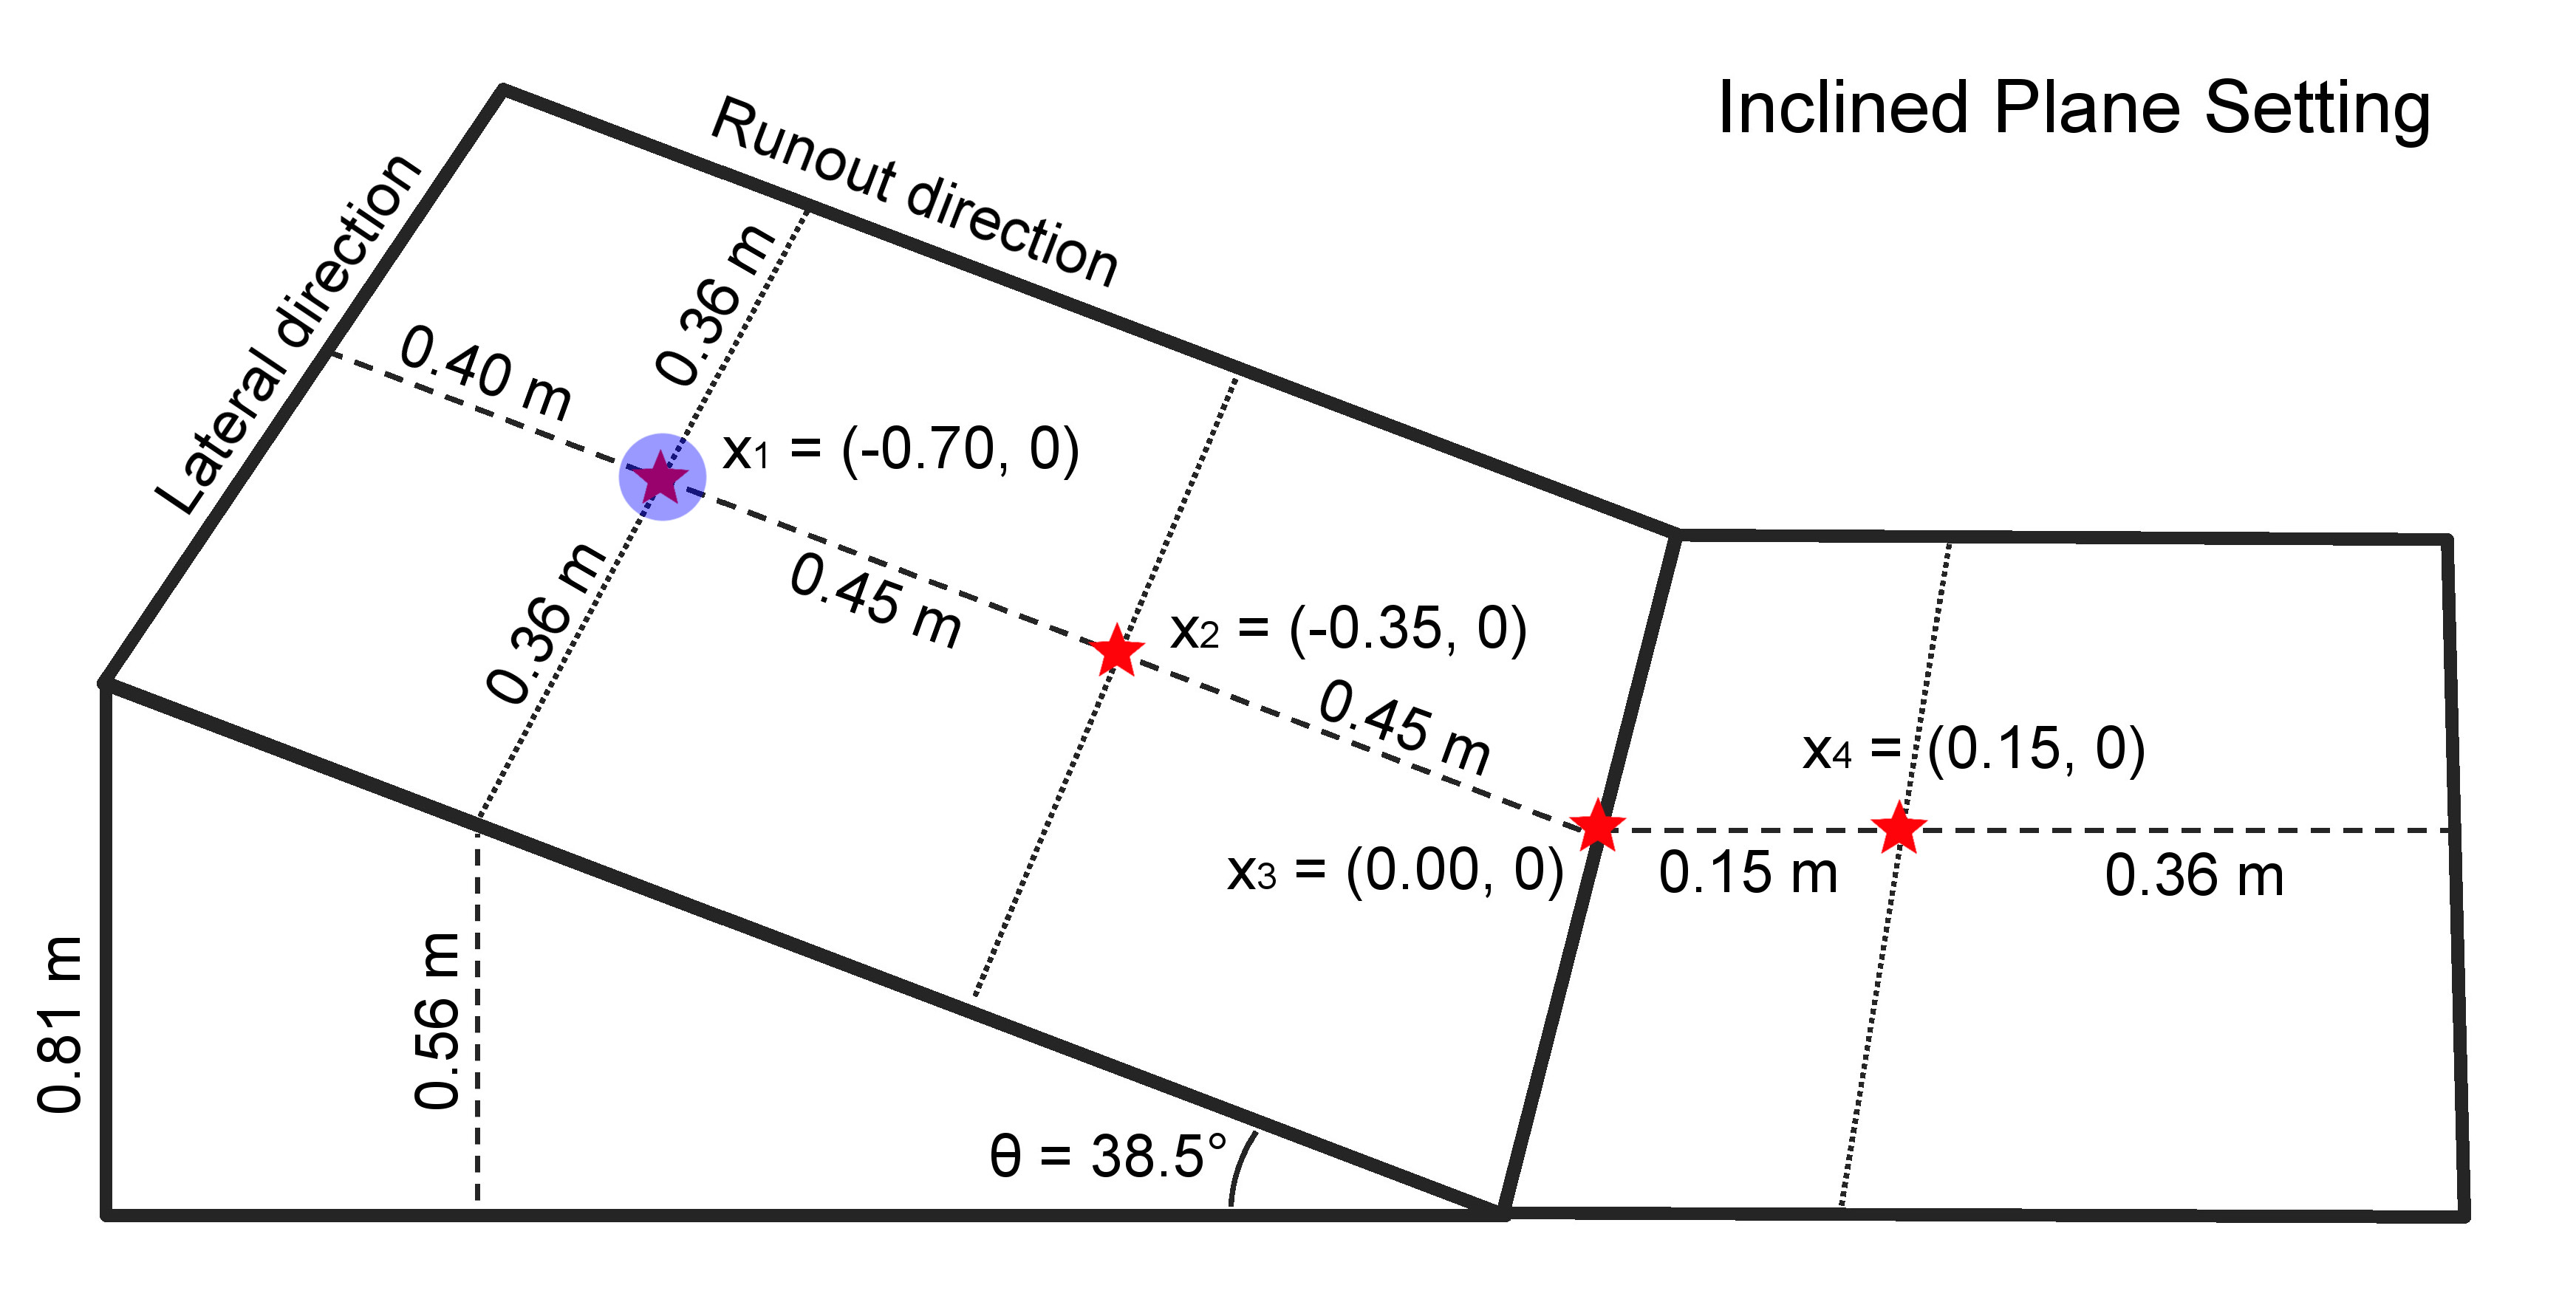
\includegraphics[width=0.8\textwidth]{inclPlaneFig.jpg}
    \centering
    \caption{Inclined plane description, including local samples sites (red stars). Pile location is marked by a blue dot.}
    \label{fig:Ramp-first}
\end{figure}

A second case study is a block and ash flow down the slope of Volc{\'a}n de Colima (M{\'e}xico) - an andesitic stratovolcano that rises to 3,860 m above sea level, situated in the western portion of the Trans-Mexican Volcanic Belt (Fig. \ref{fig:Colima-first}). Historically, it has been the most active volcano in M{\'e}xico \citep{DeLaCruzReina1993, Zobin2002, Gonzalez2002}. During July 10$^{th}$-11$^{th}$ 2015, the volcano underwent its most intense eruptive phase since its Subplinian-Plinian 1913 AD eruption \citep{Saucedo2010, Zobin2015, ReyesDaVilla2016, Capra2016}. The modeling of pyroclastic flows generated by explosive eruptions and lava dome collapses of Volc{\'a}n de Colima is a well studied problem \citep{DelPozzo1995,Sheridan1995,Saucedo2002,Saucedo2004,Saucedo2005, Sarocchi2011, Capra2015}. The volcano has been already used as a case study in several research involving the Titan2D code \citep{Rupp2004, Rupp2006, Dalbey2008, Yu2009, Sulpizio2010, Capra2011, Aghakhani2016}.

In this study the flow is assumed to be generated by the gravitational collapse of a paraboloid dome placed close to the summit area. A dome collapse occurs when there is a significant amount of recently-extruded highly-viscous lava piled up in an unstable configuration around a vent. Further extrusion and/or externals forces can cause the still hot dome of viscous lava to collapse, disintegrate, and avalanche downhill \citep{Bursik2005}. The hot, dense blocks in this ``block and ash'' flow will typically range from centimeters to a few meters in size. The matrix is composed of fine ash from the comminuted blocks. Computations were performed on a DEM with 5m-pixel resolution, obtained from LiDAR data acquired in 2005 \citep{Davila2007, Sulpizio2010}.

\begin{figure}[H]
    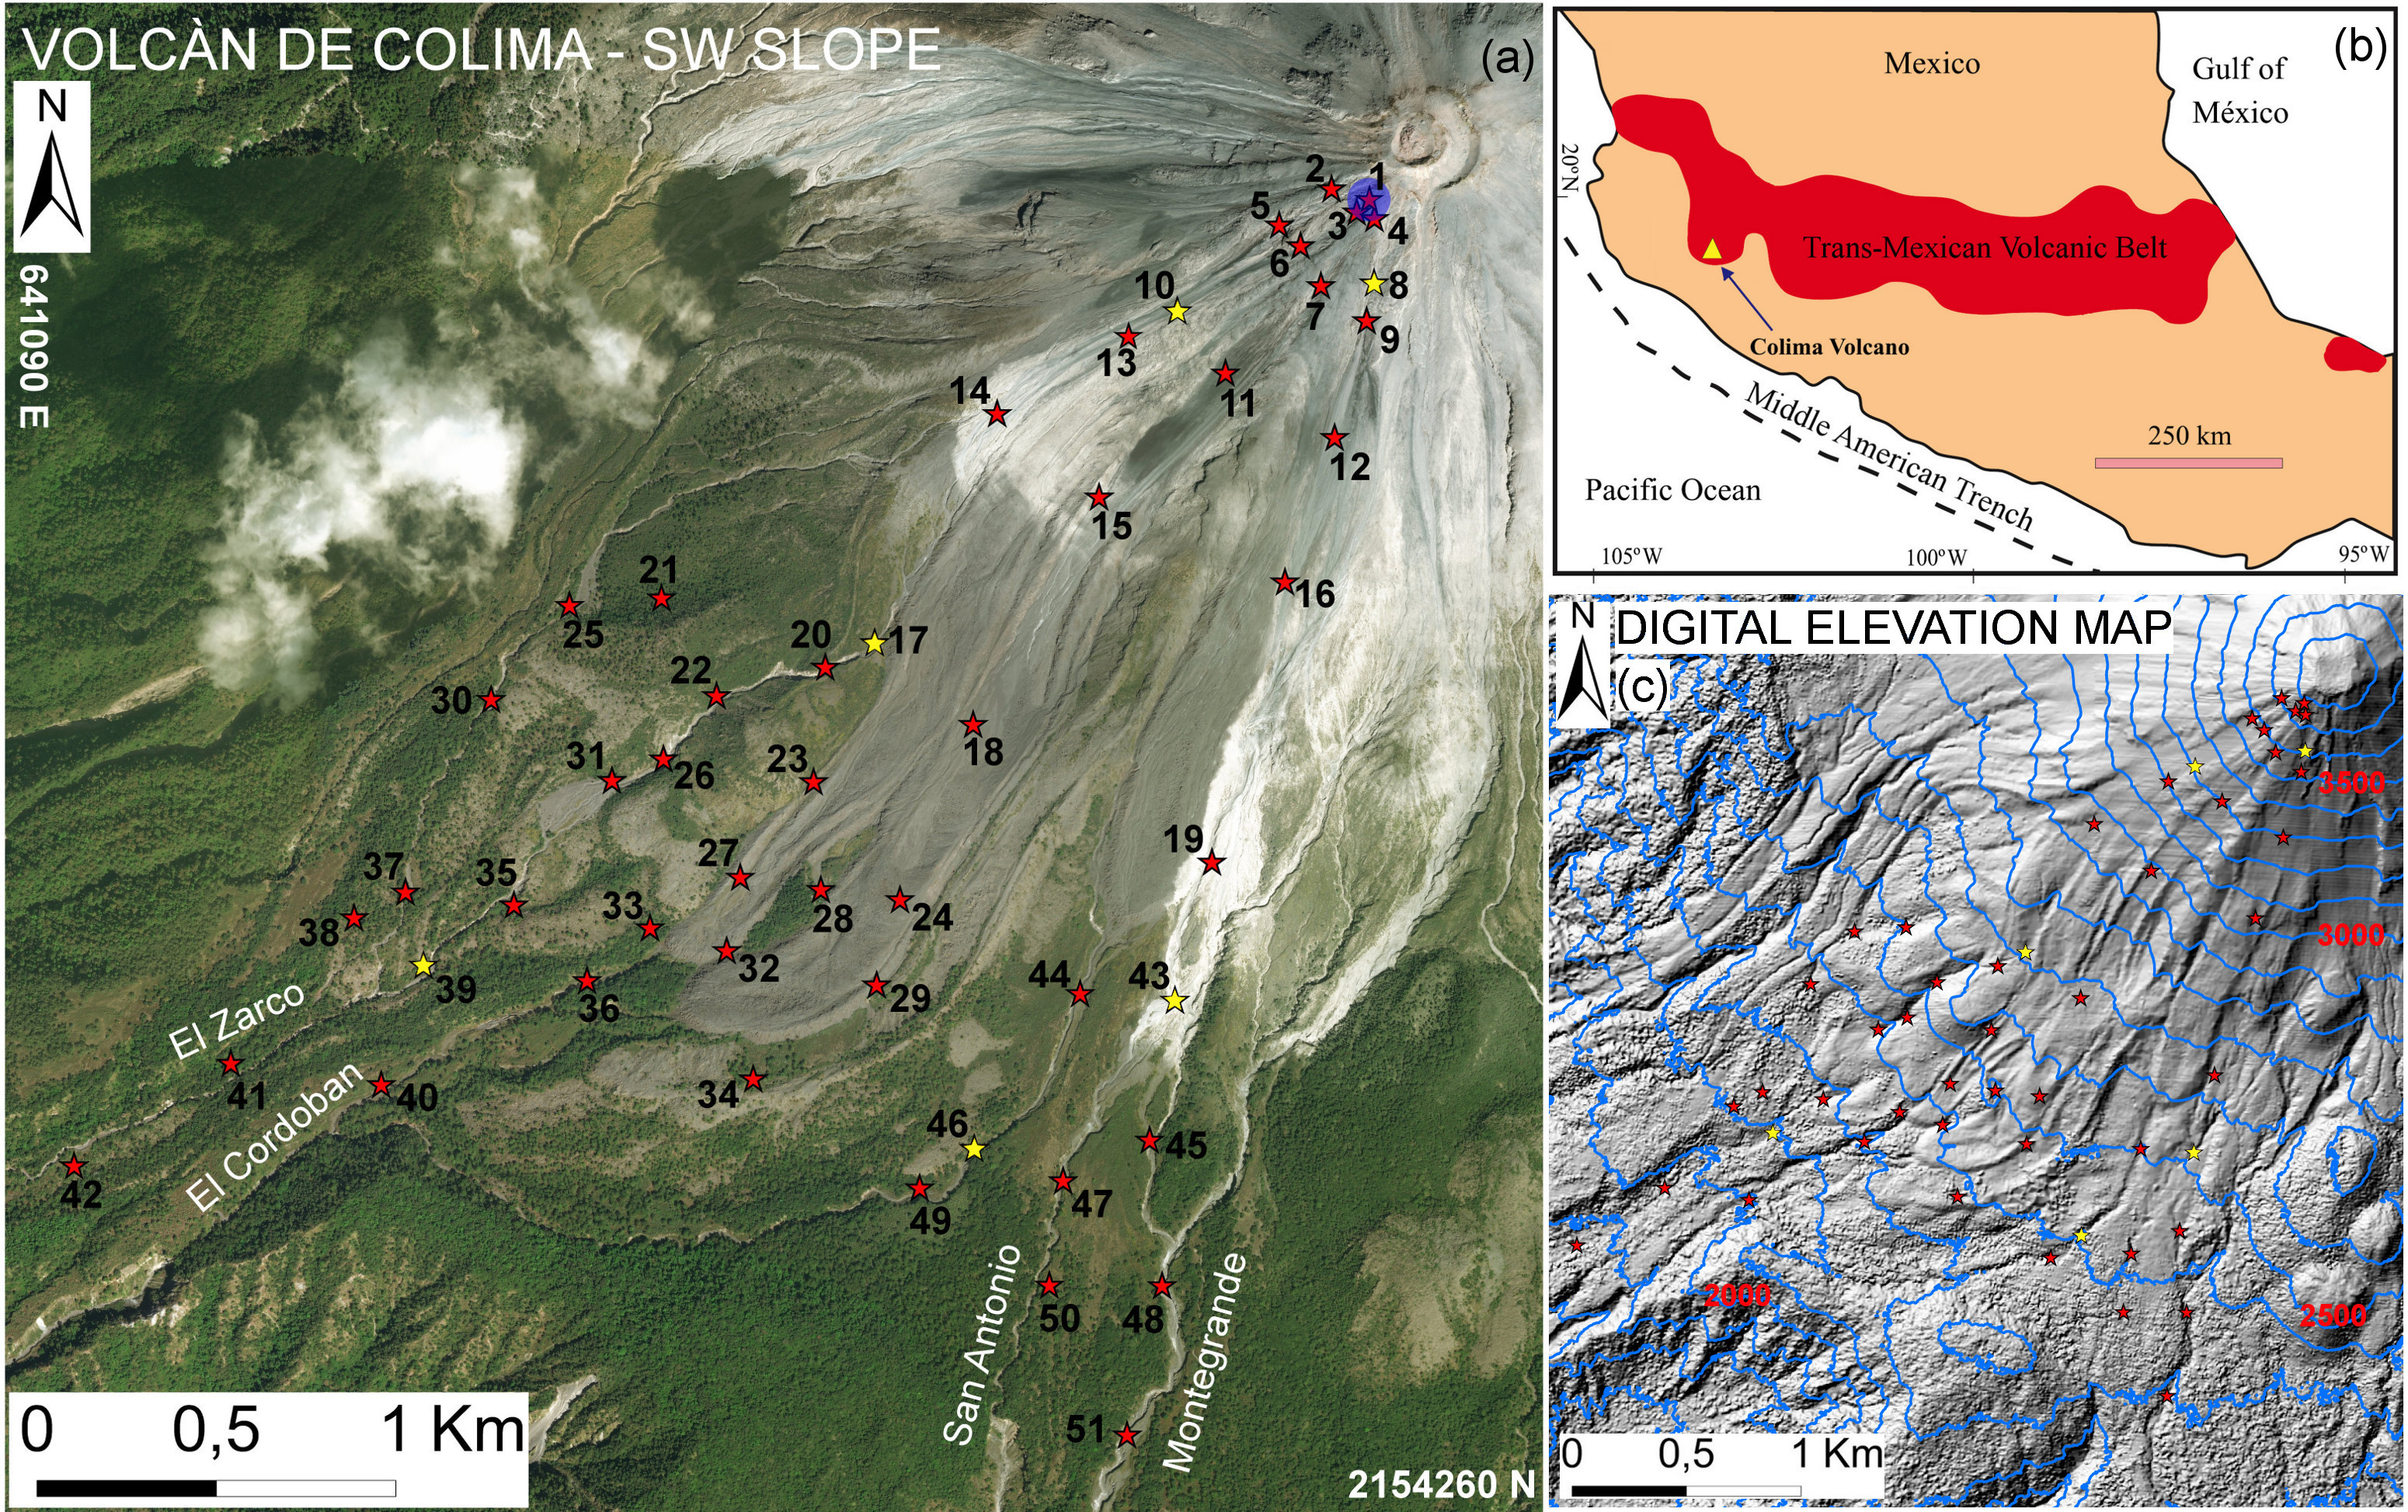
\includegraphics[width=0.9\textwidth]{ColimaFig.jpg}
    \centering
    \caption{Volc{\'a}n de Colima (M{\'e}xico) overview, including 51 numbered local sample sites (red stars) and four labeled major ravines channeling the flow. Pile location is marked by a blue dot. Reported coordinates are in UTM zone 13N. Digital elevation map and regional geology map are also displayed.}
    \label{fig:Colima-first}
\end{figure}

\section{Overview of the models}\label{sec:GeoPhFlows}

\subsection{Modeling Assumptions}\label{subsec:ModelAssump}
The models of geophysical mass flows described in this study rely on several physical and mathematical assumptions. We will classify them in two groups - the general assumptions and the rheology assumptions. The main focus of this study is on the latter group, but, in principle, the same procedure could be applied to the former.

\paragraph{General Assumptions}
\begin{itemize}
\item The \textit{shallowness} approximation is at the base of the depth-averaging procedure. In this approximation, the flow depth is assumed to be at least an order of magnitude less than the characteristic length of the flowing material. Variation of velocity within the flow depth is neglected.

\item The material is assumed to be \textit{continuous}. The real flows consist of granular material and, sometimes, interstitial fluid. Usually the ``typical particle'' diameter is small compared to the depth and length of the flowing mass, and the rheological properties are imposed to approximate the bulk behavior that is expected of an actual mass flow.

\item The moving mass is assumed to be \textit{volume preserving}. In contrast, phenomena of erosion and deposition of material may violate this assumption.

\item The flowing mass is assumed to be consisted of an \textit{incompressible} fluid. This means that we are ignoring variations of density due to the void ratio (i.e. the density is uniform in space and time).

\item The body of mass is supposed to be in \textit{isothermal} state or, if not, thermal effects can be ignored.

\item The mass flow is assumed to be \textit{free surface}. Air entrainment is instead frequently observed in the dilute real flows.

\item The stress tensor is \textit{symmetric} w.r.t. the \textit{z} axis.
\end{itemize}

The shallowness assumptions is very important, and brings several implications which may be considered additional assumptions on their own.

\paragraph{Consequences of Shallowness}
\begin{itemize}
\item The shallowness assumption implies a \textit{hydrostatic} expression for the normal pressure in the direction perpendicular to the basal surface. Moreover, the downslope and cross-slope pressure components are assumed to be varying linearly with the normal pressure component through the flow depth.

\item The \textit{boundary layer} where the shearing deformation takes place is collapsed to zero thickness. The sliding and shearing velocity are combined to a single sliding law with a somewhat larger modelled sliding velocity.

\item The \textit{lateral shear stresses can be neglected}, compared to the basal shear stresses. Motion of the bulk of mass consists of ``shearing within the deforming mass'' and ``sliding along the basal surface''.
\end{itemize}

The list rheology assumptions is detailed when the models are presented.



\subsection{Governing Equations and Boundary Conditions}\label{subsec:GovEqsBCs}
The motion of the mass flow is described by the basic conservation of mass and momentum for an incompressible medium \citep{Patra2005}:
\begin{eqnarray}\label{eq:N_S}
\nabla \cdot\underline{{\textbf u}} &=& 0, \nonumber \\
\dfrac{\partial}{\dt}(\rho \ \underline{{\textbf u}})+\nabla \cdot (\rho \ \underline{{\textbf u}}\otimes \underline{{\textbf u}}) &=& \nabla \cdot \underline{\underline{{\mathbf{T}}}}+\rho \ \underline{{\textbf g}},
\end{eqnarray}
Where $\underline{{\textbf u}}=[u, v, w]^{\mathrm{T}}$ is the material velocity in cartesian coordinates, $\rho$ is its constant density, $\underline{\underline{{\mathbf{T}}}}$ is the \textit{Cauchy} stress tensor, and $\underline{{\textbf g}}$ is the gravity acceleration vector.

The Cauchy stress tensor, $\underline{\underline{{\mathbf{T}}}}$, depends on the rheology assumptions. The kinetic boundary conditions are defined on the free surface $F^s=s(x,y,t)-z=0$ and basal surface $F^b=b(x,y,t)-z=0$ interfaces:
\begin{equation}\label{eq:SurKinBC}
\frac{\partial F^s}{\dt} + \underline{{\textbf u}}\cdot\nabla F^s = 0, \ \ at \ F^s(x,y,t)=0
\end{equation}
\begin{equation}\label{eq:BedKinBC}
\frac{\partial F^b}{\dt} + \underline{{\textbf u}}\cdot\nabla F^b = 0, \ \ at \ F^b(x,y,t)=0
\end{equation}

The depth-averaged Saint-Venant equations that TITAN2D solves are:
\begin{eqnarray}
\label{eq:D_A}
\frac{\partial h}{\partial t} +
\frac{\partial}{\partial x}(h \bar{u}) +
\frac{\partial}{\partial y}(h\bar{v}) &=& 0, \nonumber \\
\frac{\partial}{\partial t} (h\bar{u}) +
\frac{\partial}{\partial x}\left(h\bar{u}^2 + \frac{1}{2}k g_{z}h^2\right) + \frac{\partial}{\partial y}(h\bar{u}\bar{v}) &=& S_{x},\\
\frac{\partial}{\partial t} (h\bar{v}) +
\frac{\partial}{\partial x}(h\bar{u}\bar{v}) +
\frac{\partial}{\partial y}\left(h\bar{v}^2 + \frac{1}{2}k g_{z}h^2\right) &=& S_{y}\nonumber
\end{eqnarray}
Here the cartesian coordinate system is aligned such that $z$ is normal to the surface; $h$ is the flow height in the $z$ direction; $h\bar{u}$ and $h\bar{v}$ are respectively the components of momentum in the $x$ and $y$ directions; and $k$ is the coefficient which relates the lateral stress components, $\bar{\sigma}_{xx}$ and $\bar{\sigma}_{yy}$, to the normal stress component, $\bar{\sigma}_{zz}$. The definition of this coefficient depends on the constitutive model of the flowing material we choose. Note that $\frac{1}{2} k g_z h^2$ is the contribution of hydrostatic pressure to the momentum fluxes. $S_x$ and $S_y$ are the sum local stresses: they include the gravitational driving forces the basal friction force resisting to the motion of the material, and additional forces specific of rheology assumptions.

\subsubsection{Numerical solver}\label{NumS}
Let $\textbf{U}=\left[h, \ h\bar{u}, \ h\bar{v}\right]^T$ be the vector of conservative variables and $\textbf{F}=\left[h\bar{u}, \ h\bar{u}^2+0.5 k_{ap} g_z h^2, \ h\bar{v}\bar{u}\right]^T$ and $\textbf{G}=\left[h\bar{v}, \ h\bar{u}\bar{v}, \ h\bar{v}^2+0.5 k_{ap} g_z h^2\right]^T$ be the physical flux vectors.
In order to solve the system of hyperbolic conservation laws (\ref{eq:D_A}), TITAN2D employs a finite volume Godunov solver, and the time-stepping procedure is achieved by an explicit Euler scheme \citep{Pitman2003a, Patra2005, Patra2006}. Assuming $\textbf{S}=\left[S_h, \ S_x, \ S_y\right]^T$ as the source terms vector containing the effect of the flow rheology, the flow in the next time step updates as:
\begin{equation}\label{integrator}
\textbf{U}_{i,j}^{n+1} = \textbf{U}_{i,j}^n - \frac{\bigtriangleup t}{\bigtriangleup x} \{\textbf{F}_{i+\frac{1}{2},j}^n - \textbf{F}_{i-\frac{1}{2},j}^n \} - \frac{\bigtriangleup t}{\bigtriangleup y} \{\textbf{G}_{i,j+\frac{1}{2}}^n - \textbf{G}_{i,j-\frac{1}{2}}^n \} + \bigtriangleup t \ \textbf{S}_{i,j}
\end{equation}
Where $\textbf{F}_{i\pm\frac{1}{2},j}^n$ and $\textbf{G}_{i,j\pm\frac{1}{2}}^n$ are the numerical flux terms at the inter-cell boundaries which are computed regarding the Harten-Lax-Van Leer Riemann solver \citep{Toro2013} . In fact, the evolution of the flow to the next time step depends on the advection flux at the cell interface, which results from the wave interaction at the boundaries between cells.
On the other hand, adaptive mesh refinement allows for the concentration of computing power on regions of special interest. It captures the complex flow features along the flow boundaries, as well as the locations where there are large mass or momentum fluxes (which may include places where the topography changes abruptly). Mesh coarsening is also applied where the solution values are relatively constant or small to further improve the computational efficiency \citep{Patra2005,Aghakhani2016}.

\subsection{Rheology assumptions}\label{subsec:Models}
In the three following sections, we briefly describe \emph{Mohr-Coulomb} (MC), \emph{Pouliquen-Forterre} (PF) and \emph{Voellmy-Salm} (VS) models.

\subsubsection{Mohr-Coulomb model}\label{MCM}
Based on the long history of studies in soil mechanics \cite{Rankine1857}, the Mohr-Coulomb rheology model was developed and used to represent the behavior of geophysical mass flows \cite{SavageHutter1989}.

Shear and normal stress are assumed to obey Coulomb friction equation, both within the flow and at its boundaries. In other words,
\begin{equation}
\tau = \sigma \tan \phi,
\end{equation}
where $\tau$ and $\sigma$ are respectively the shear and normal stresses on failure surfaces, and $\phi$ is a friction angle. This relationship does not depend on the magnitude of flow speed.

Under the assumption of symmetry of the stress tensor w.r.t. the \textit{z} axis, the earth pressure coefficient $k=k_{ap}$ can take on only one of three values indicated by the square dots shown in Figure \ref{mohr_circle}. The material yield criterion is represented by the two straight lines at angles $\pm \phi$ (the internal friction angle) relative to horizontal direction. Similarly, the normal and shear stress at the bed are represented by the line $\tau=-\sigma \tan(\delta)$ where $\delta$ is the bed friction angle. The three possible stress states in the \textit{xz}-plane are indicated by the square dots. The circular dots show the additional possible stress states for $\sigma_{yy}$ for a non-axisymmetric stress tensor.

Regarding the friction angle stated above, we have two material properties in this model:
\begin{itemize}
\item Internal friction angle, $\phi_{int}$, which resists material shear.
\item Bed friction angle, $\phi_{bed}$, which resists motion of the material relative to the bed. This is a joint property of the material and the surface it flows over.
\end{itemize}
It is worth mentioning that the effective value of the friction angles can be strongly reduced by the presence of interstitial fluid, sometimes creating modeling issues. Specific models have been developed in case the effect of interstitial fluid is believed to be particularly relevant \citep{PitmanLe2005}.

\paragraph{Earth pressure coefficient} $k=k_{ap}$ is defined in MC as:
\begin{eqnarray}\label{k_ap}
k_{ap} = \begin{cases}
\frac{\sigma_{xx}^{b \ act}}{\sigma_{zz}^b}=2\frac{1-\sqrt{1-\cos^2(\phi_{int})(1+\tan^2 (\phi_{bed}))}}{\cos^2(\phi_{int})}-1, & \nabla \cdot \underset{^\sim}{\bar{\textbf u}}>0, \ active\\
\frac{\sigma_{xx}^{b}}{\sigma_{zz}^b}=1, & \nabla \cdot \underset{^\sim}{\bar{\textbf u}}=0, \ neutral\\
\frac{\sigma_{xx}^{b \ pass}}{\sigma_{zz}^b}=2\frac{1+\sqrt{1-\cos^2(\phi_{int})(1+\tan^2 (\phi_{bed}))}}{\cos^2(\phi_{int})}-1, & \nabla \cdot \underset{^\sim}{\bar{\textbf u}}<0, \ passive
\end{cases}
\end{eqnarray}

\begin{figure}[H]
        \centering
        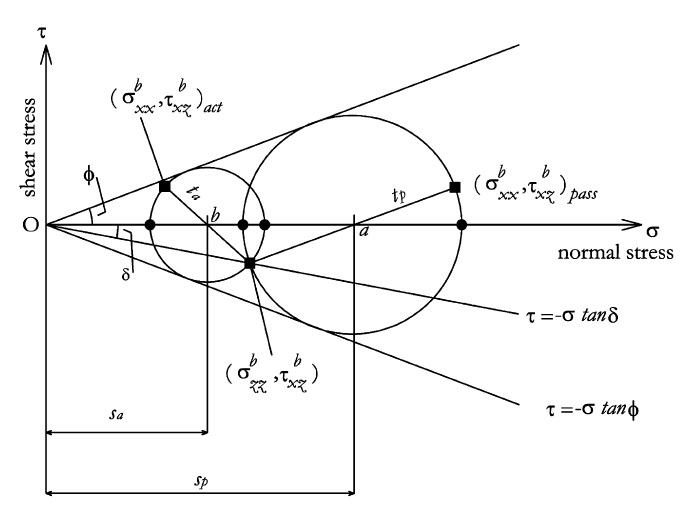
\includegraphics[width=.7\textwidth]{Figures/mohr.jpg}
        \caption{Mohr-circle-diagram representing the stress state within a granular medium \cite{Pirulli2007}.}
        \label{mohr_circle}
\end{figure}

\paragraph{MC equations} As a result, we can write down the source terms of the Eqs. (\ref{eq:D_A}):
\begin{eqnarray}
S_x = g_x h  - \frac{\bar{u}}{\| \underset{^\sim}{\bar{\textbf u}} \|} \left[h\left(g_z+\frac{\bar{u}^2}{r_x}\right)\tan(\phi_{bed})\right] - h k_{ap} \ {\rm sgn}\left(\frac{\partial \bar{u}}{\partial y}\right) \frac{\partial (g_z h)}{\partial y} \sin(\phi_{int}),\nonumber \\
S_y = g_y h  - \frac{\bar{v}}{\| \underset{^\sim}{\bar{\textbf u}} \|} \left[h\left(g_z +\frac{\bar{v}^2}{r_y}\right)\tan(\phi_{bed})\right] - h k_{ap} \ {\rm sgn}\left({\frac{\partial \bar{v}}{\partial x}}\right) \frac{\partial (g_z h)}{\partial x} \sin(\phi_{int})
\end{eqnarray}
Where, $\underset{^\sim}{\bar{\textbf u}} = (\bar{u} , \bar{v})$, is the depth-averaged velocity vector, $r_x$ and $r_y$ denote the radii of curvature
of the local basal surface. It is possible to approximate the inverse of the radii of curvature by the partial derivatives of the basal slope, e.g., $1/r_x = \partial \theta_x/\partial x$, where $\theta_x$ is the local bed slope.

\paragraph{MC rheology assumptions} In summary:
\begin{itemize}
\item \textit{Basal Friction} is based on a constant friction angle.

\item \textit{Internal Friction} gives a not negligible contribution and it is based on a constant friction angle.

\item \textit{Earth pressure coefficient} formula depending on the Mohr-Coulomb circle.

\item Velocity based \textit{curvature effects} are included into the equations.
\end{itemize}

\subsubsection{Pouliquen-Forterre model}\label{PFM}
The scaling properties for granular flows down rough inclined planes led to a new formulation of the basal friction stress as a function of the flow depth and velocity \cite{Pouliquen1999}.

Two critical slope inclination angles are defined as functions of the flow thickness, namely $\phi_{start}(h)$ and $\phi_{stop}(h)$. The function $\phi_{stop}(h)$ gives the slope angle at which a steady uniform flow leaves a deposit of thickness $h$, while $\phi_{start}(h)$ is the angle at which a layer of thickness $h$ is mobilized. They define two different basal friction coefficients:
\begin{eqnarray}
\mu_{start}(h)=\tan(\phi_{start}(h))\\
\mu_{stop}(h)=\tan(\phi_{stop}(h))
\end{eqnarray}

An empirical friction law $\mu_{b}(\|\underset{^\sim}{\bar{\textbf{u}}} \| , h)$ is then defined in the whole range of velocity and thickness. The expression changes depending on two flow regimes, according to a parameter $\beta$ and the Froude number $Fr=\| \underset{^\sim}{\bar{\textbf{u}}} \| / \ \sqrt{h g_{z}}$.

\paragraph{Dynamic friction regime - $Fr \geq \beta$}
\begin{equation}\label{mu_beta1}
\mu(h, Fr)=\mu_{stop}(h \beta / Fr)
\end{equation}

\paragraph{Intermediate friction regime - $0 < Fr < \beta$}
\begin{equation}\label{mu_beta2}
\mu(h, Fr)=\left(\frac{Fr}{\beta}\right)^\gamma [\mu_{stop}(h)-\mu_{start}(h)] + \mu_{start}(h),
\end{equation}
where $\gamma=10^{-3}$ is the power of extrapolation chosen in \cite{PouliquenForterre2002}. In particular, if $Fr=\beta$, then $\mu(h, Fr)=\mu_{stop}(h)$, and if $Fr = 0$, then $\mu(h, Fr)=\mu_{start}(h)$.

The functions $\mu_{stop}$ and $\mu_{start}$ are defined by:
\begin{equation}\label{mu-stop}
\mu_{stop}(h)=\tan\phi_{1} + \frac{\tan\phi_{2}-\tan\phi_{1}}{1+h/\it \mathcal{L}}
\end{equation}
and
\begin{equation}\label{mu-start}
\mu_{start}(h)=\tan\phi_{3} + \frac{\tan\phi_{2}-\tan\phi_{1}}{1+h/\it \mathcal{L}}
\end{equation}
The critical angles $\phi_{1}$, $\phi_{2}$ and $\phi_{3}$ and the parameters $\mathcal{L}, \beta$ are the material properties.

In particular, $\mathcal{L}$ is the characteristic depth of the flow over which a transition between the angles $\phi_{1}$ to $\phi_{2}$ occurs, in the $\mu_{stop}$ formula. In practice, if $h\ll \mathcal L$, then $\mu_{stop}(h)\approx \tan\phi_{2}$, and if $h\gg \mathcal L$, then $\mu_{stop}(h)\approx\tan\phi_{1}$. The effect of the topographic local curvatures is also taken into account.

\paragraph{PF equations} The depth-averaged Eqs. (\ref{eq:D_A}) source terms take the following form:
\begin{eqnarray}\label{eq:S_Pouliquen}
S_{x} &=&  g_{x} h -  \frac{\bar{u}}{\| \underset{^\sim}{\bar{\textbf{u}}} \|}\left[h \left(g_z+\frac{\bar{u}^2}{r_x}\right) \ \mu_{b}(\|\underset{^\sim}{\bar{\textbf{u}}} \| , h)\right] \ + g_{z}h\frac{\partial h}{\partial x} \nonumber \\
S_{y} &=&  g_{y} h - \frac{\bar{v}}{\| \underset{^\sim}{\bar{\textbf{u}}} \|}\left[h \left(g_z +\frac{\bar{v}^2}{r_y}\right) \ \mu_{b}(\|\underset{^\sim}{\bar{\textbf{u}}} \| , h)\right] \ + g_{z}h\frac{\partial h}{\partial y}
\end{eqnarray}

\paragraph{PF rheology assumptions} In summary:
\begin{itemize}
\item \textit{Basal Friction} is based on an interpolation of different friction angles, based on the flow regime and depth.

\item \textit{Internal Friction} is neglected.

\item \textit{Earth pressure coefficient} is equal to one.

\item Normal stress is modified by a \textit{hydrostatic pressure force} related to the flow height gradient.

\item Velocity based \textit{curvature effects} are included into the equations.
\end{itemize}



\subsubsection{Voellmy-Salm model}\label{VSM}
The theoretical analysis of dense snow avalanches led to the VS rheology model \citep{Voellmy1955, Salm1993}. The following relation between shear and normal stresses holds:
\begin{equation}
\tau = \mu \sigma + \frac{\rho \| \underset{^\sim}{\textbf g} \|}{\xi} \| \underset{^\sim}{\bar{\textbf u}} \|^2,
\end{equation}
where, $\sigma$ denotes the normal stress at the bottom of the fluid layer and $\underset{^\sim}{\textbf g} = (g_{x} , g_{y} , g_{z})$ represents the gravity vector. The VS rheology adds a velocity dependent \emph{turbulent} friction to the traditional velocity independent basal friction term which is proportional to the normal stress at the flow bottom. The two parameters of the model are the bed friction coefficient $\mu$ and the turbulent friction coefficient $\xi$. By dimension analysis, $\xi$ is equivalent to an acceleration, while $\mu$ is dimensionless. The division of the total basal friction into velocity independent and dependent parts allows the modeling of avalanche behavior when the avalanche is flowing with a high velocity in the acceleration zone and close to stopping in the runout zone.

The effect of the topographic local curvatures is again taken into account by adding the terms containing the local radii of curvature $r_x$ and $r_y$. In this case the formula is considering the modulus of velocity instead than the scalar component \citep{Fischer2012}.

\paragraph{VS equations} Therefore, the final source terms take the following form:
\begin{eqnarray}
\label{eq:S_terms_curv}
S_{x} &=&  g_{x} h - \frac{\bar{u}}{\| \underset{^\sim}{\bar{\textbf u}}\|} \ \left[ h \left(g_{z} + \frac{\| \underset{^\sim}{\bar{\textbf u}} \|^2}{r_{x}} \right)\mu+ \frac{\| \underset{^\sim}{\textbf g} \|}{\xi}\| \underset{^\sim}{\bar{\textbf u}} \|^2\right], \nonumber \\
S_{y} &=& g_{y} h - \frac{\bar{v}}{\| \underset{^\sim}{\bar{\textbf u}}\|} \ \left[ h \left(g_{z} + \frac{\| \underset{^\sim}{\bar{\textbf u}} \|^2}{r_{y}} \right)\mu+ \frac{\| \underset{^\sim}{\textbf g} \|}{\xi}\| \underset{^\sim}{\bar{\textbf u}} \|^2\right]
\end{eqnarray}

\paragraph{VS rheology assumptions} In summary:
\begin{itemize}
\item \textit{Basal Friction} is based on a constant coefficient, similarly to the MC rheology.

\item \textit{Internal Friction} is neglected.

\item \textit{Earth pressure coefficient} is equal to one.

\item Additional \textit{turbulent friction} is based on the local velocity by a quadratic expression.

\item Velocity based \textit{curvature effects} are included into the equations, following an alternative formulation.
\end{itemize}


\section{UQ Process}
The key purpose of this study is to present a procedure for the improved exploration and quantitative comparison of physical models and their assumptions through the collection of full statistical data. Models are not black boxes, behind each physical model there are different physical assumptions, and therefore it would be more appropriate to look at those instead than at the entire model results. Our statistical approach enables a first step towards a data driven selection of the best modeling assumptions to use.

In particular, a good forecasting capability in the context of mass flows requires the careful selection of the pair $(M(A), P(M(A)))$, where $A$ is a set of assumptions, $M(A)$ is the model which combines those assumptions, and $P(M)$ is a probability distribution in the parameter space of $M$. An assumption is a quite general concept - for example it can be a specific equation for the internal stress, the implementation of bed curvature effects, of active-passive material stretching, or the use of a specific correction on the pressure effects, etc... Assumptions are what makes the models being different, and each model may be seen as the combined result of a set of assumptions. Sometimes a good model contains a useless assumption that may be removed, sometimes a good assumption should be implemented inside a different model - those are usually considered as subjective choices, not data driven. Moreover, the correct assumptions may change through time, making the analysis more difficult.

It is worth mentioning that whereas the support of $P(M)$ can be restricted to a single point in case an optimization procedure is performed for the reconstruction of a particular flow, this is not possible if we are interested in the general predictive capabilities of the model, i.e. what is desired in probabilistic hazard assessment. In this study we will always assume $P(M)\sim \bigotimes_{i=1}^{N_M} Unif(a_{i,M},b_{i,M})$, where $N_M$ is the number of parameters of $M$. These parameter ranges will not be selected under the influence of a particular observation, but we will try to use the information gathered in literature about the physical meaning of those values.

In general, the simulation algorithms can be classified as:
$$\textmd{(1)INPUT VARIABLES} \longrightarrow \textmd{(2)DYNAMICAL QUANTITIES} \longrightarrow \textmd{(3)OBSERVABLE OUTPUTS}$$

The input variables can include: volume, rheology coefficients, initiation site and geometry, digital elevation map. We will focus on the former two of those, the volume of the pile and the rheology, which constitute our parameter space in all the case studies. The dynamical quantities are directly related to the force terms in the Newton Equations that rule the simulation, they include: driving and dissipative stresses and powers. The terms of the equations are hidden to the observation, but they directly depend on the parameters, and represent a fundamental link between the parameters and the observable outputs. Moreover, the models share some of those terms while change others, and this enables a detailed comparison of the real physics below the curtain. Finally, the observable outputs include: flow height, inundated area, flow velocity and acceleration. In the sequel (2) and (3) are also called quantities of interest (QoI).

Another level of complexity can be achieved choosing the degree of integration of (2) and (3) in the previous scheme:
\begin{description}
  \item[(A)] LOCAL MEASUREMENTS
  \item[(B)] SPATIAL AVERAGES
  \item[(C)] TEMPORAL AVERAGES
  \item[(D)] SPATIO-TEMPORAL (FULL) AVERAGES
\end{description}

In particular, all the dynamical quantities, and most of the observable outputs, have a local meaning. They are calculated on the elements of the numerical mesh created by the code. Moreover, all those quantities are time dependent. Differences in time and location enable to constrain the changes in flow regime. Those are really important because if the flow behavior is radically different, then the significance and effects of the assumptions may also change.

A first approach to look at the data is to choose a reasonable design of spatial locations and to calculate the graph of the quantities as a function of time. A second approach is to make the spatial integral of those quantities and calculate their temporal graph - this integration can be done with respect to the basal area, e.g. for the stresses and related powers, or with respect to the flow volume, e.g. velocity and acceleration. A third possible approach requires to make the integrals through time at each designed spatial site, a fourth approach the full integral in space-time.

In general, for each QoI and degree of integration, during a Monte Carlo simulation we sample the input variables and obtain a family of temporal graphs in (A), (B), and numeric values in (C), (D). These results are statistically summarized - plotting their expectation, their standard deviation, their 5th and 95 percentiles. Their correlation structure is also explored, presenting the plots of the Pearson coefficients of the most interesting pairs of quantities in (1), (2), (3). In the following, we will detail the considered input variables and quantities of interest for each of our cases study.

Our sampling technique of the input variables is based on the Latin Hypercube Sampling (LHS) idea, and in particular, on the improved space-filling properties of the orthogonal array-based Latin Hypercubes (see Appendix A). The LHS is performed over $[0,1]^3$ for the MC and VS input parameters, and $[0,1]^4$ for PF input parameters. Those samples are homothetically transformed to fill the required intervals.

\subsection{Definition and consistency of the Input parameters}
In general, the three rheologies considered in this study, MC, PF, and VS, have different parameters, but in all them it is defined a basal friction stress $F$. That is $F=\tan(\phi_{bed})$ in MC, $F=\tan(\phi_2)$ for $Fr\gg h$ in PF, $F=\mu$ in VS. We use those relations to define parameter spaces which produce reasonably consistent ranges of basal frictions. In the following sections, we start defining a range for $\phi_{bed}$ of MC, specific of the scenario and obtained from the more rich literature of that rheology, then we impose a consistent range for the related parameters of PF and VS, and leave the other parameters unchanged. In particular:

\vskip.3cm\noindent \textbf{MC}
\par\noindent $\phi_{bed} \in [a, b]$, depending on the case study.
\par\noindent $\phi_{int}-\phi_{bed}=\Delta \phi \in [2^{\mathrm{\circ}}, 10^{\mathrm{\circ}}]$, following \cite{Dalbey2008}, but 25\% enlargement on the higher side of the uncertainty range.

\vskip.3cm\noindent \textbf{PF}
\par\noindent $\phi_2 = \phi_{bed}$, but with $\sim$20\% enlargement on the higher side of the uncertainty range.
\par\noindent $\phi_2-\phi_1=\Delta \phi_{12} \in [5^{\mathrm{\circ}}, 15^{\mathrm{\circ}}]$ (\cite{ForterrePouliquen2003} assumed 11$^\mathrm{\circ}$, \cite{ForterrePouliquen2003} 12$^\mathrm{\circ}$,16$^\mathrm{\circ}$; \cite{Gray2014} 9$^\mathrm{\circ}$, \cite{Barker2015} 11$^\mathrm{\circ}$).
\par\noindent $\beta \in [0.1, 0.85]$  (\cite{PouliquenForterre2002,ForterrePouliquen2003,Gray2014} assumed $\beta=0.14$ for glass beads, \cite{ForterrePouliquen2003} $\beta=0.65$ for sand)
\par\noindent $L$ is fixed and depends on the granular scale, $\phi_3=\phi_1+1^\mathrm{\circ}$ \citep{PouliquenForterre2002} due to their reduced sensitivity.

\vskip.3cm\noindent \textbf{VS}
\par\noindent $\mu = \tan(\phi_{bed})$, with $\sim$20\% enlargement of the uncertainty range.
\par\noindent $\log(\xi) \in [1.7, 4] = \log[50, 10^4]$, i.e. in this case the uniform sampling is accomplished in log-scale.

\section{QoIs and Data Collected}
\subsection{Flow down an inclined plane, and a change in slope to a flat plane}
The parameter ranges adopted in this case study are:

\vskip.3cm\noindent \textbf{MC} - $\phi_{bed} \in [15^{\mathrm{\circ}}, 30^{\mathrm{\circ}}]$ \citep{Dalbey2008}, $\quad \Delta\phi \in [2^{\mathrm{\circ}}, 10^{\mathrm{\circ}}]$.

\vskip.3cm\noindent \textbf{PF} - $\phi_2 \in [15^{\mathrm{\circ}}, 35^{\mathrm{\circ}}]$, $\quad\Delta\phi_{12} \in [5^{\mathrm{\circ}}, 15^{\mathrm{\circ}}]$, $\quad\beta \in [0.1, 0.85]$, $\quad L=10^{-3} \ (m)$, $\quad \phi_3=\phi_1 + 1^{\mathrm{\circ}}$.

\vskip.3cm\noindent \textbf{VS} - $\mu \in [0.2, 0.7]$, $\quad \log(\xi) \in [1.7, 4]$.



\subsubsection{Flow Height}

\begin{figure}[H]
	\begin{minipage}[b]{0.5\linewidth}
    	\centering
    	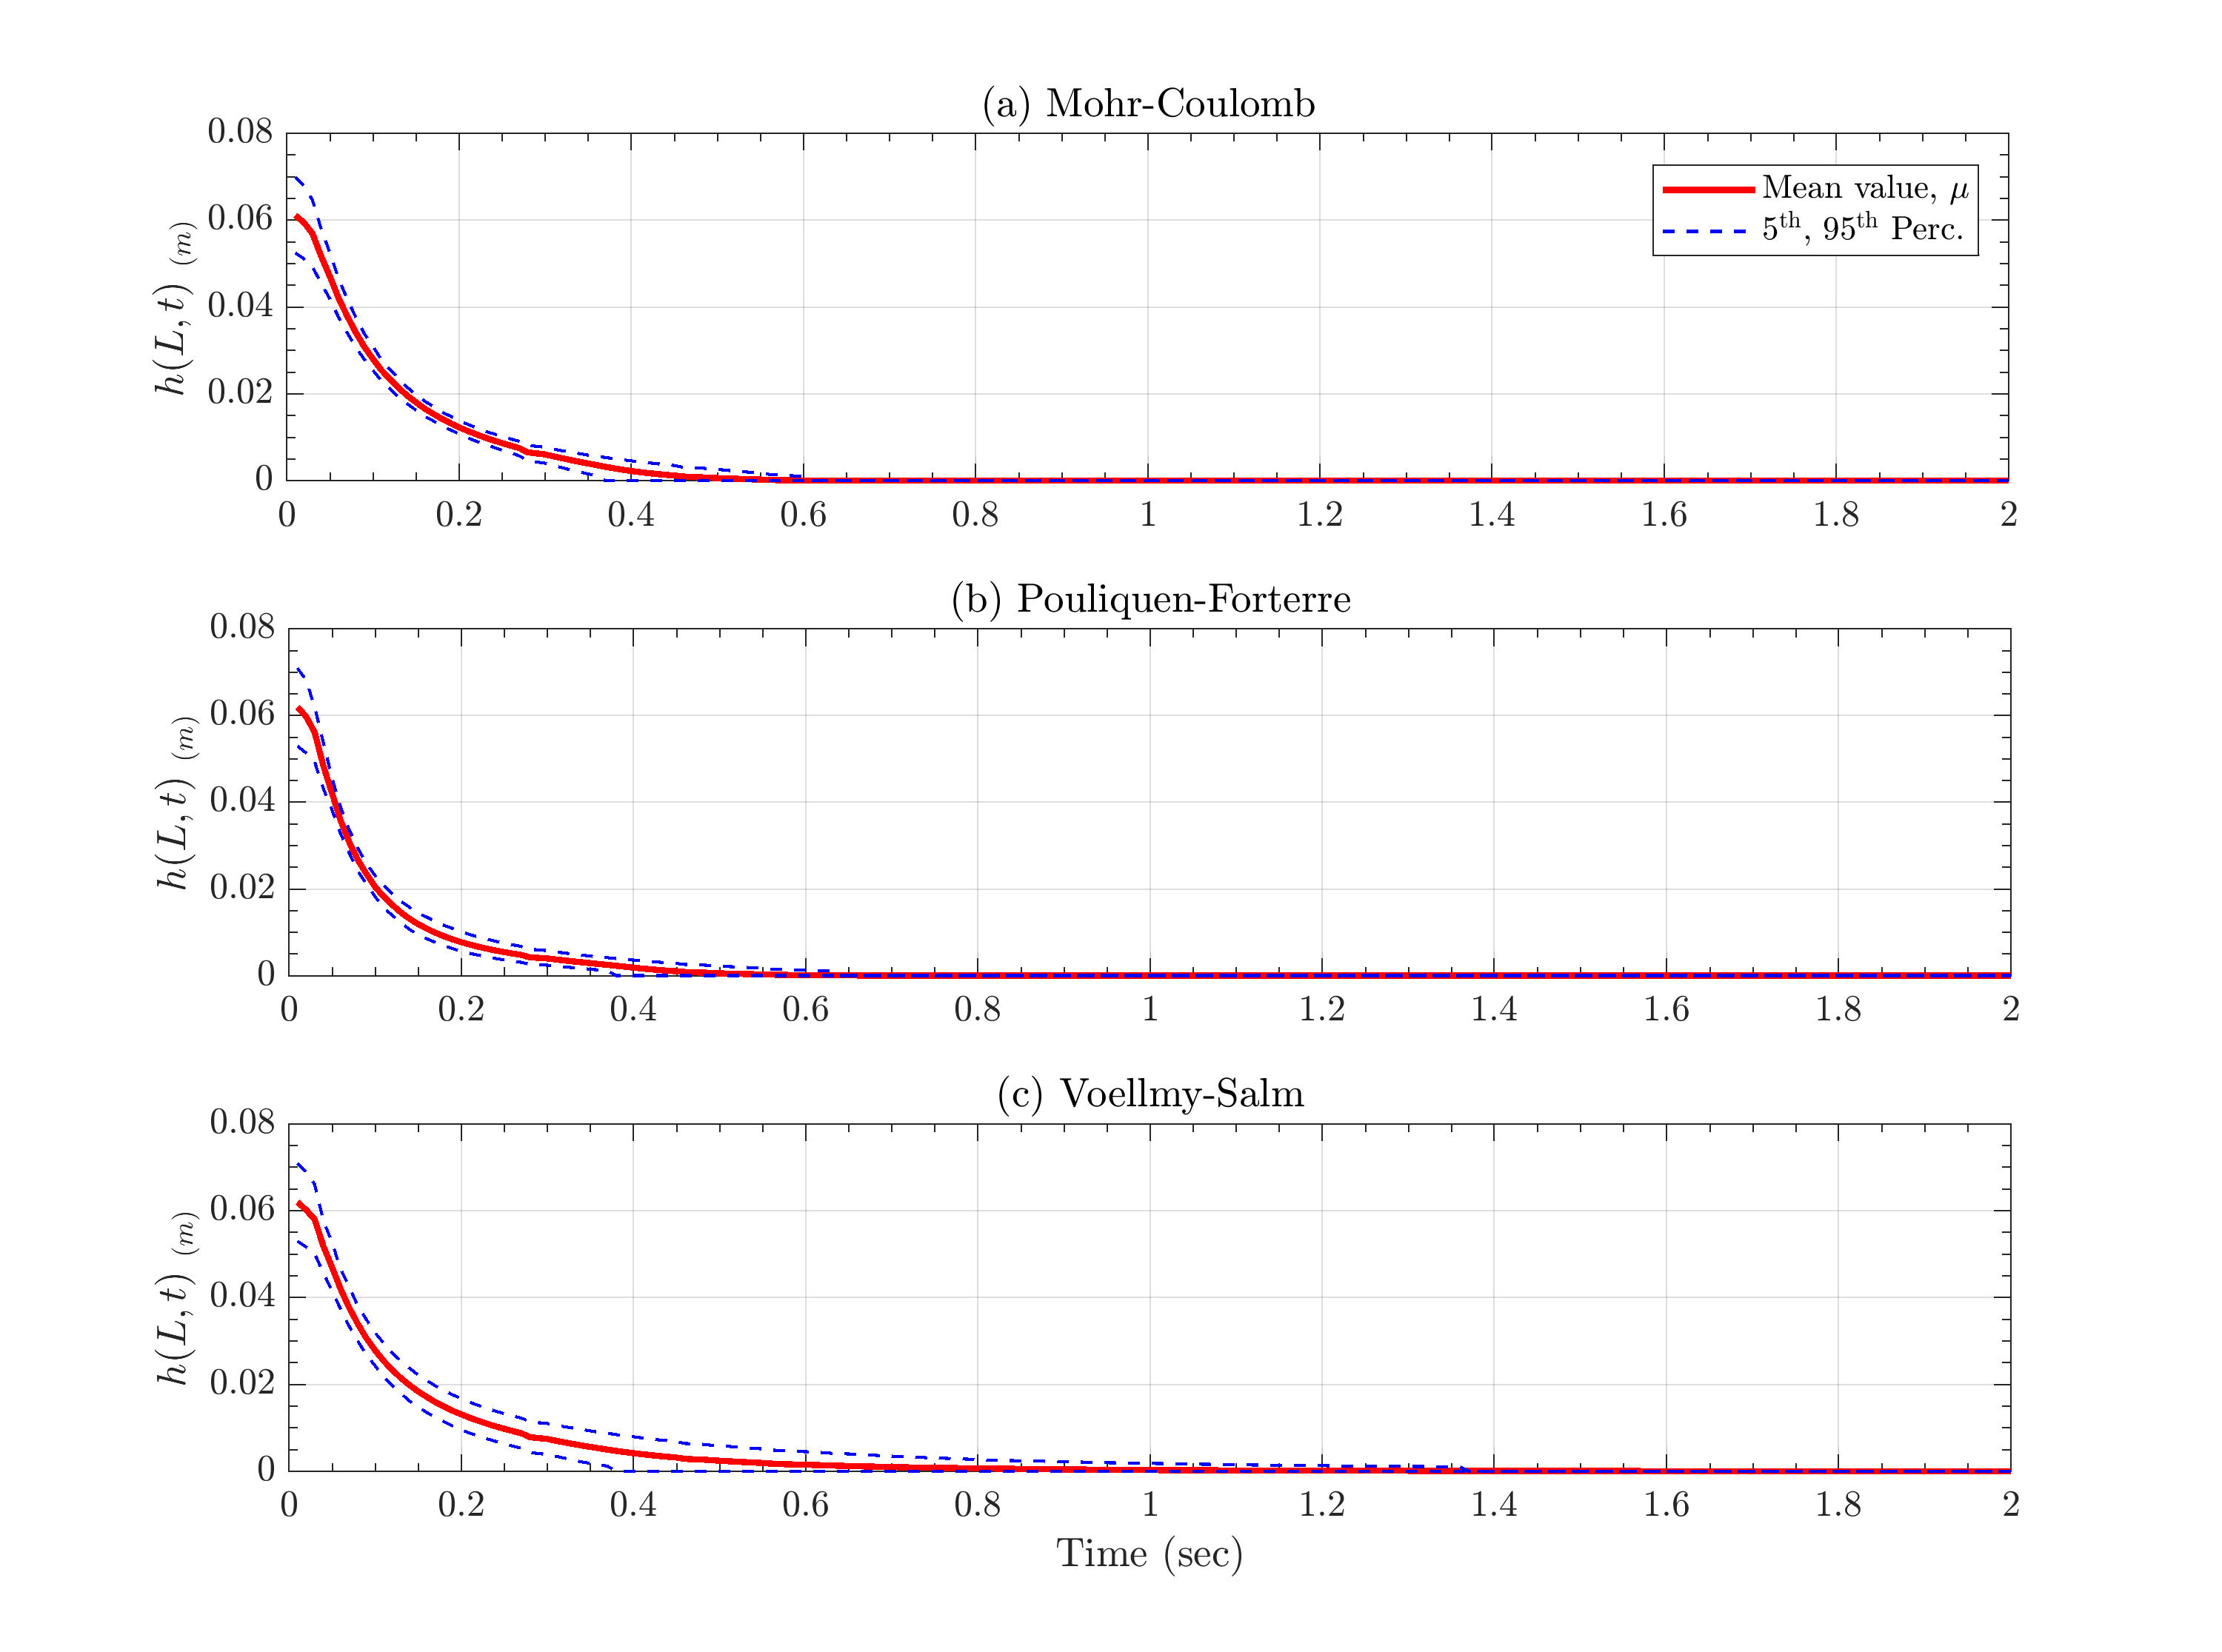
\includegraphics[width=1\textwidth]{InclinedPlane/Height/H_L1.png}
    	\subcaption{$L=(-0.7,0)$, slumping pile location.}
    	\label{fig:Ramp-L1-H}
	\end{minipage}
	\begin{minipage}[b]{0.5\linewidth}
		\centering
		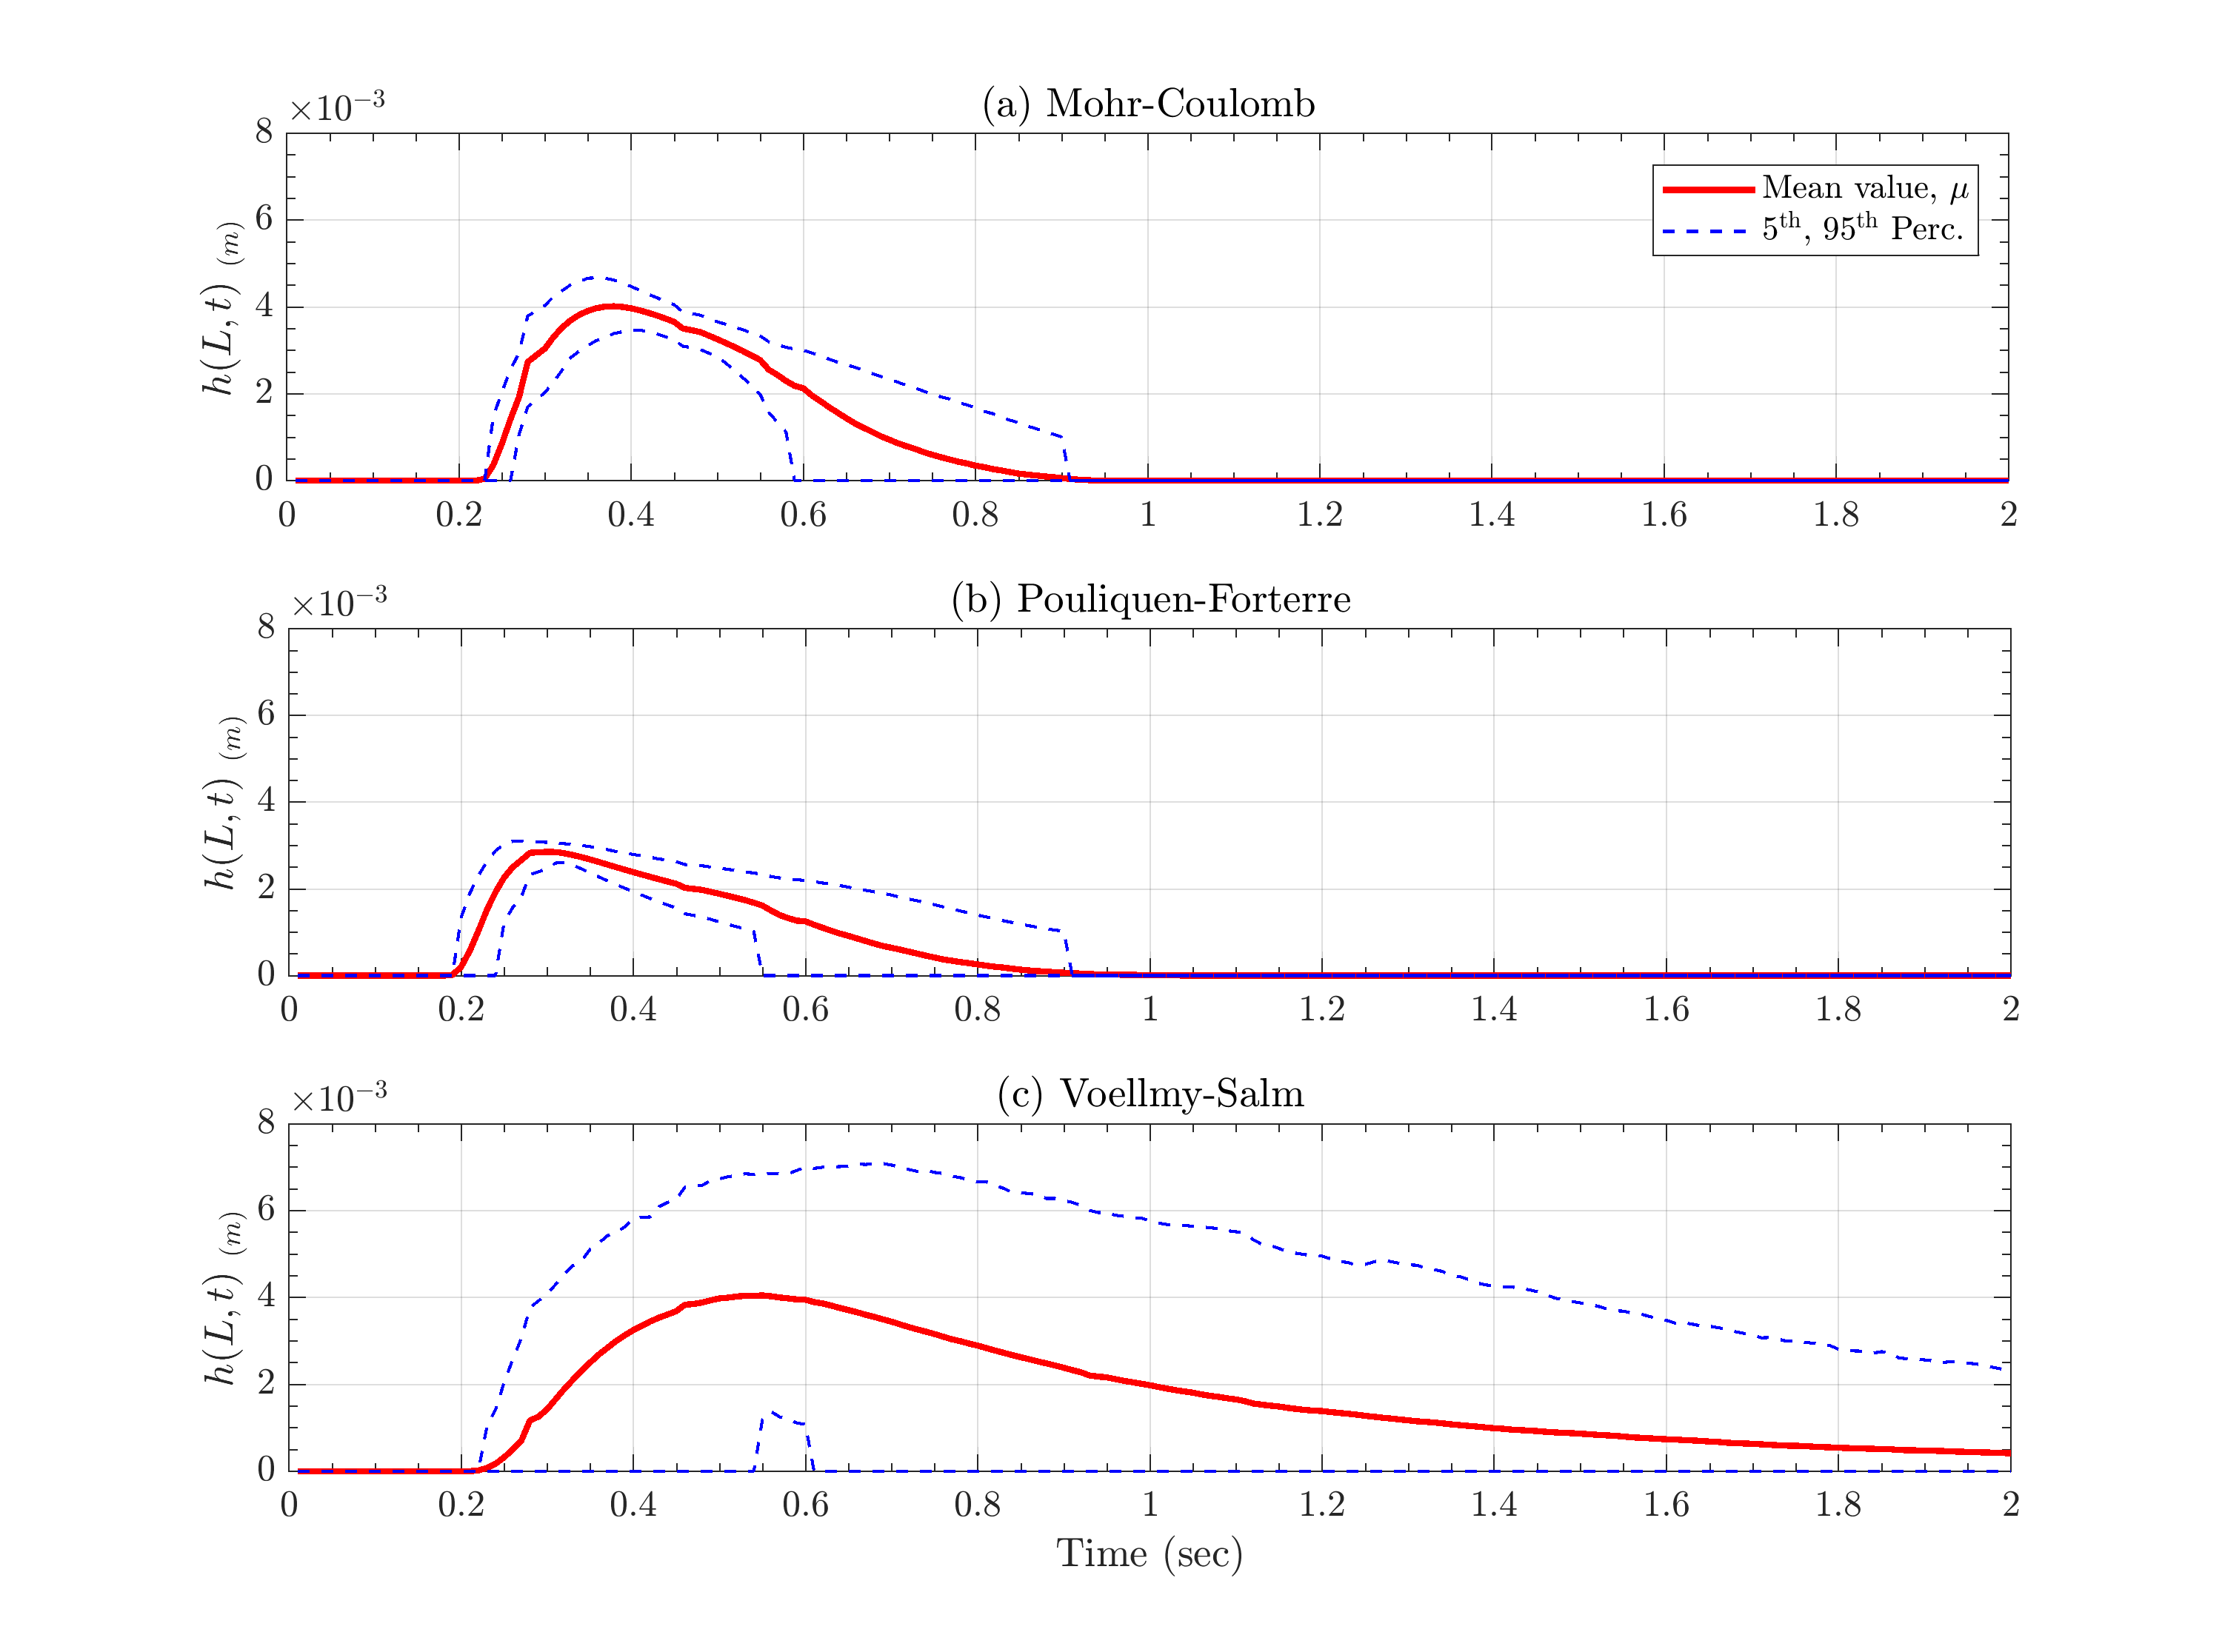
\includegraphics[width=1\textwidth]{InclinedPlane/Height/H_L2.png}
    	\subcaption{$L=(-0.35,0)$, middle point on inclined plane.}
    	\label{fig:Ramp-L2-H}
    \end{minipage}

	\begin{minipage}[b]{0.5\linewidth}
    	\centering
    	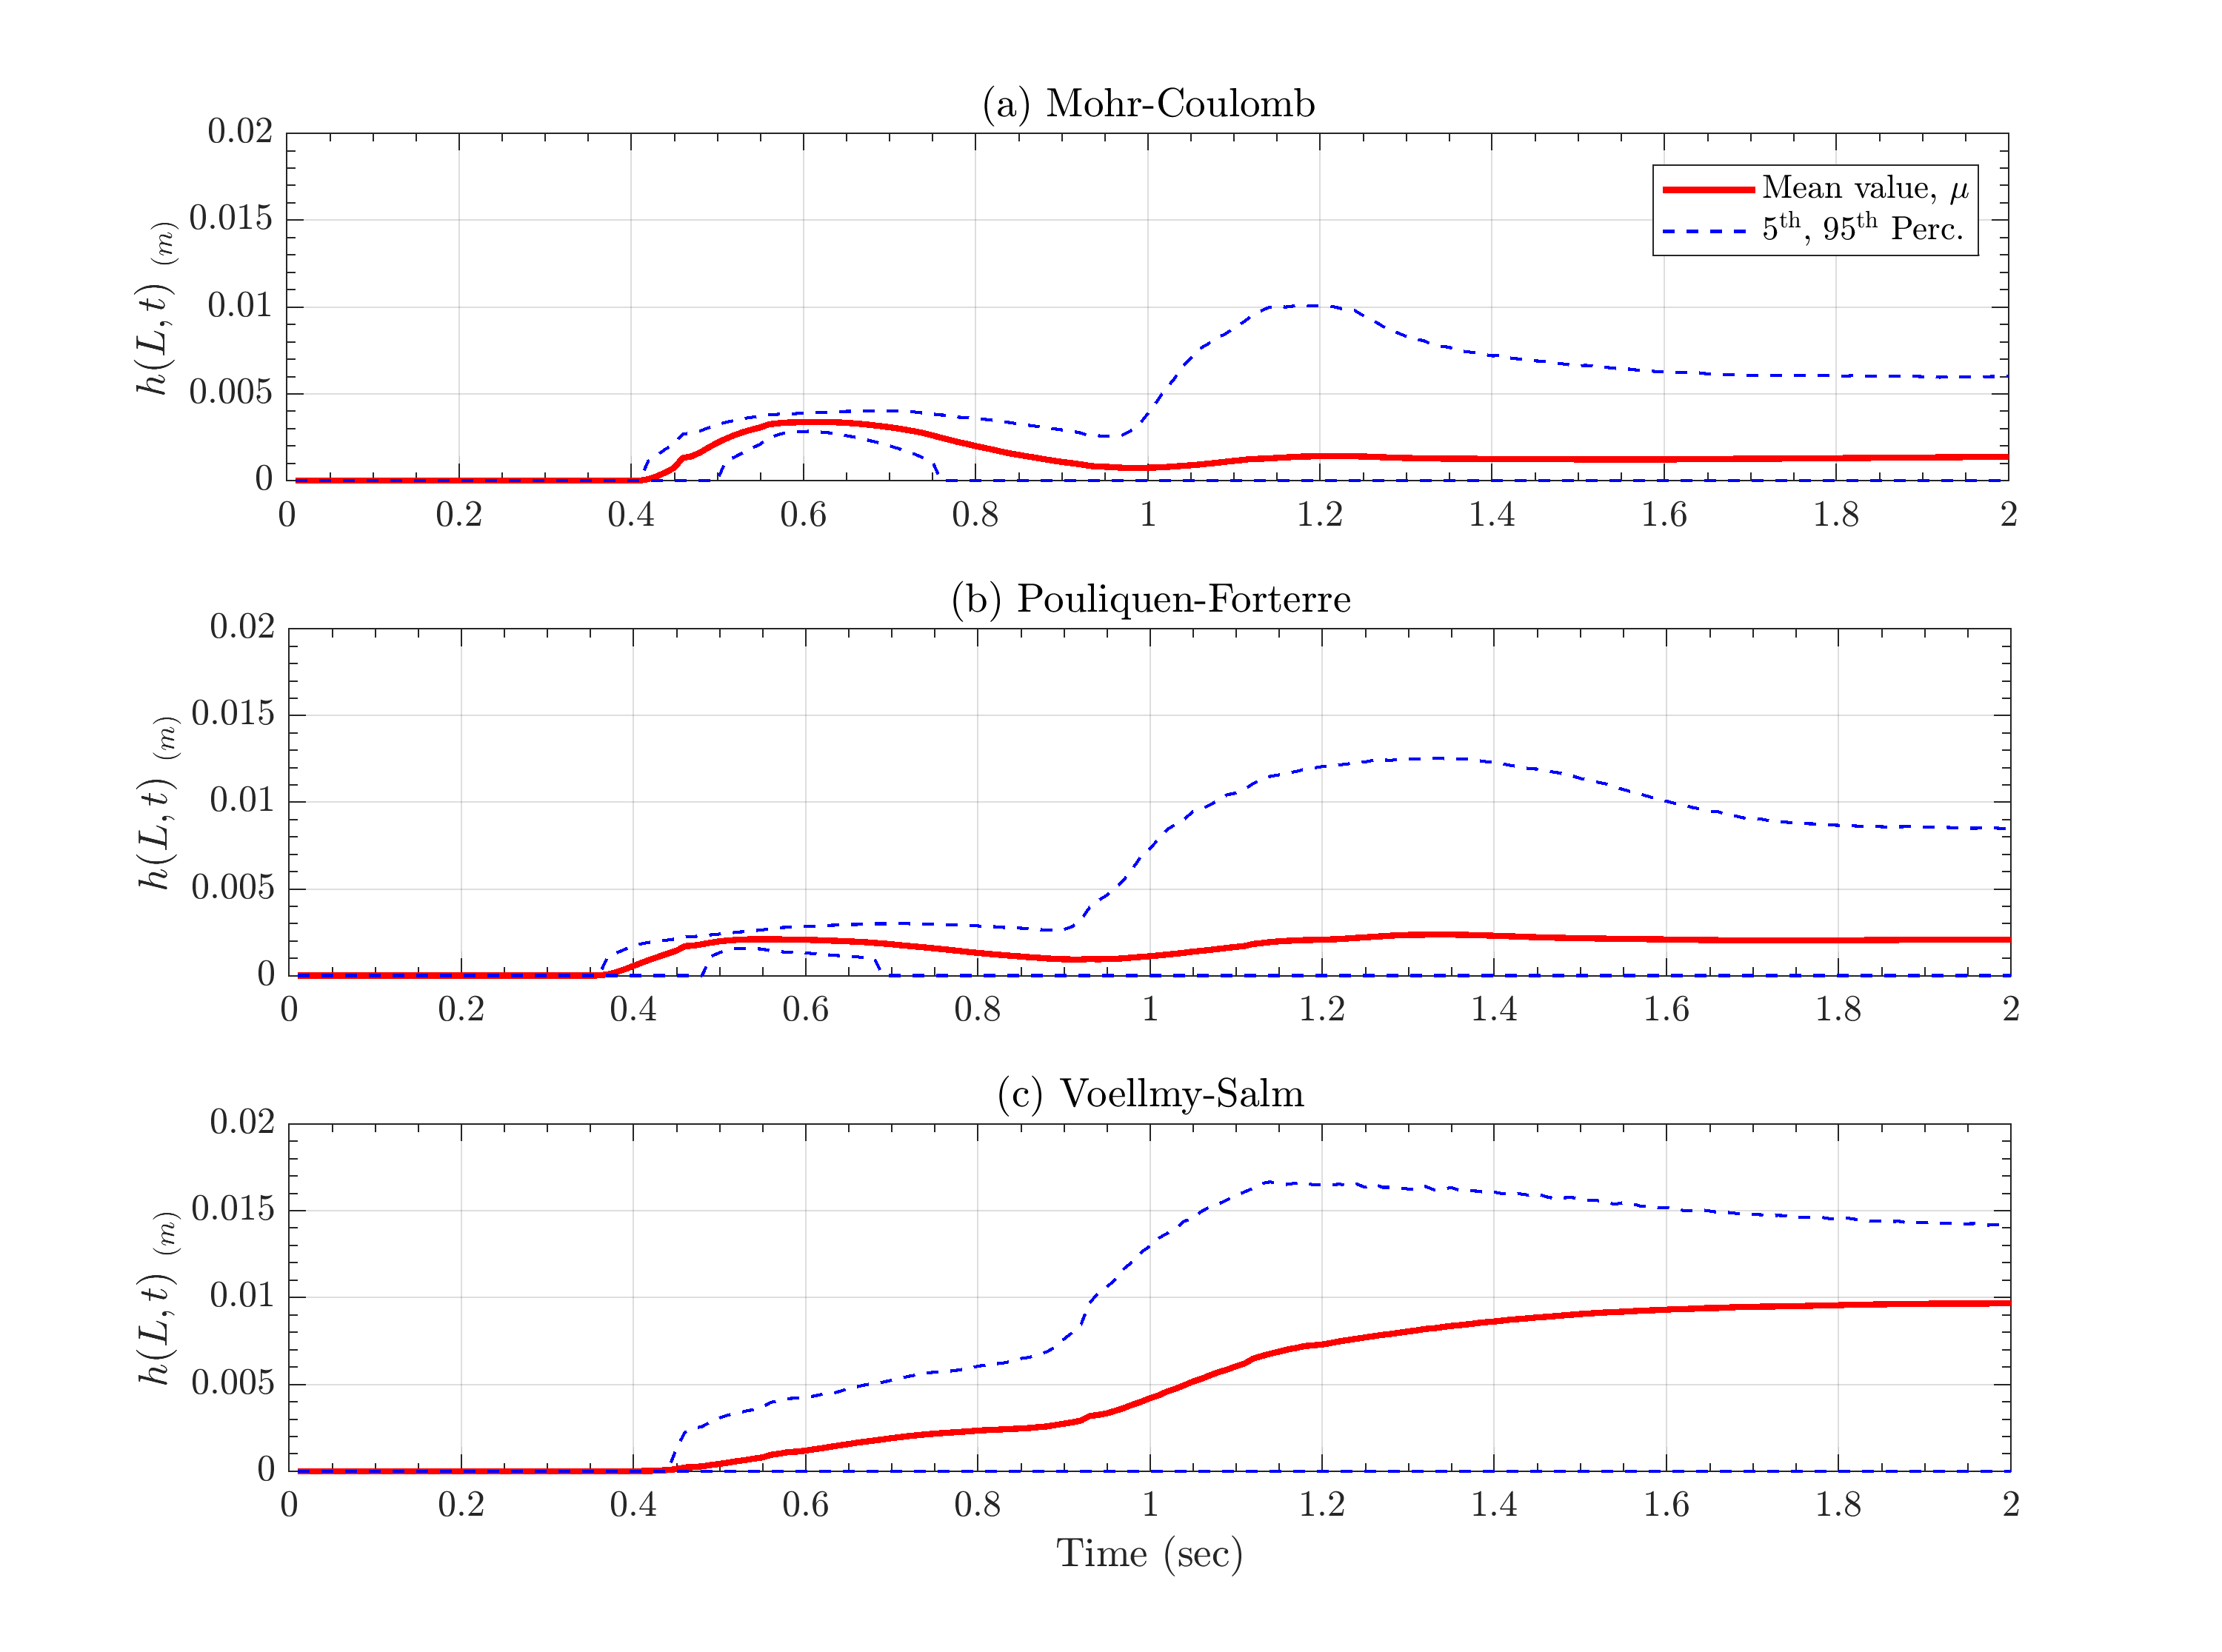
\includegraphics[width=1\textwidth]{InclinedPlane/Height/H_L3.png}
    	\subcaption{$L=(0,0)$, inclined and runout planes' joint location.}
    	\label{fig:Ramp-L3-H}
	\end{minipage}
	\begin{minipage}[b]{0.5\linewidth}
		\centering
		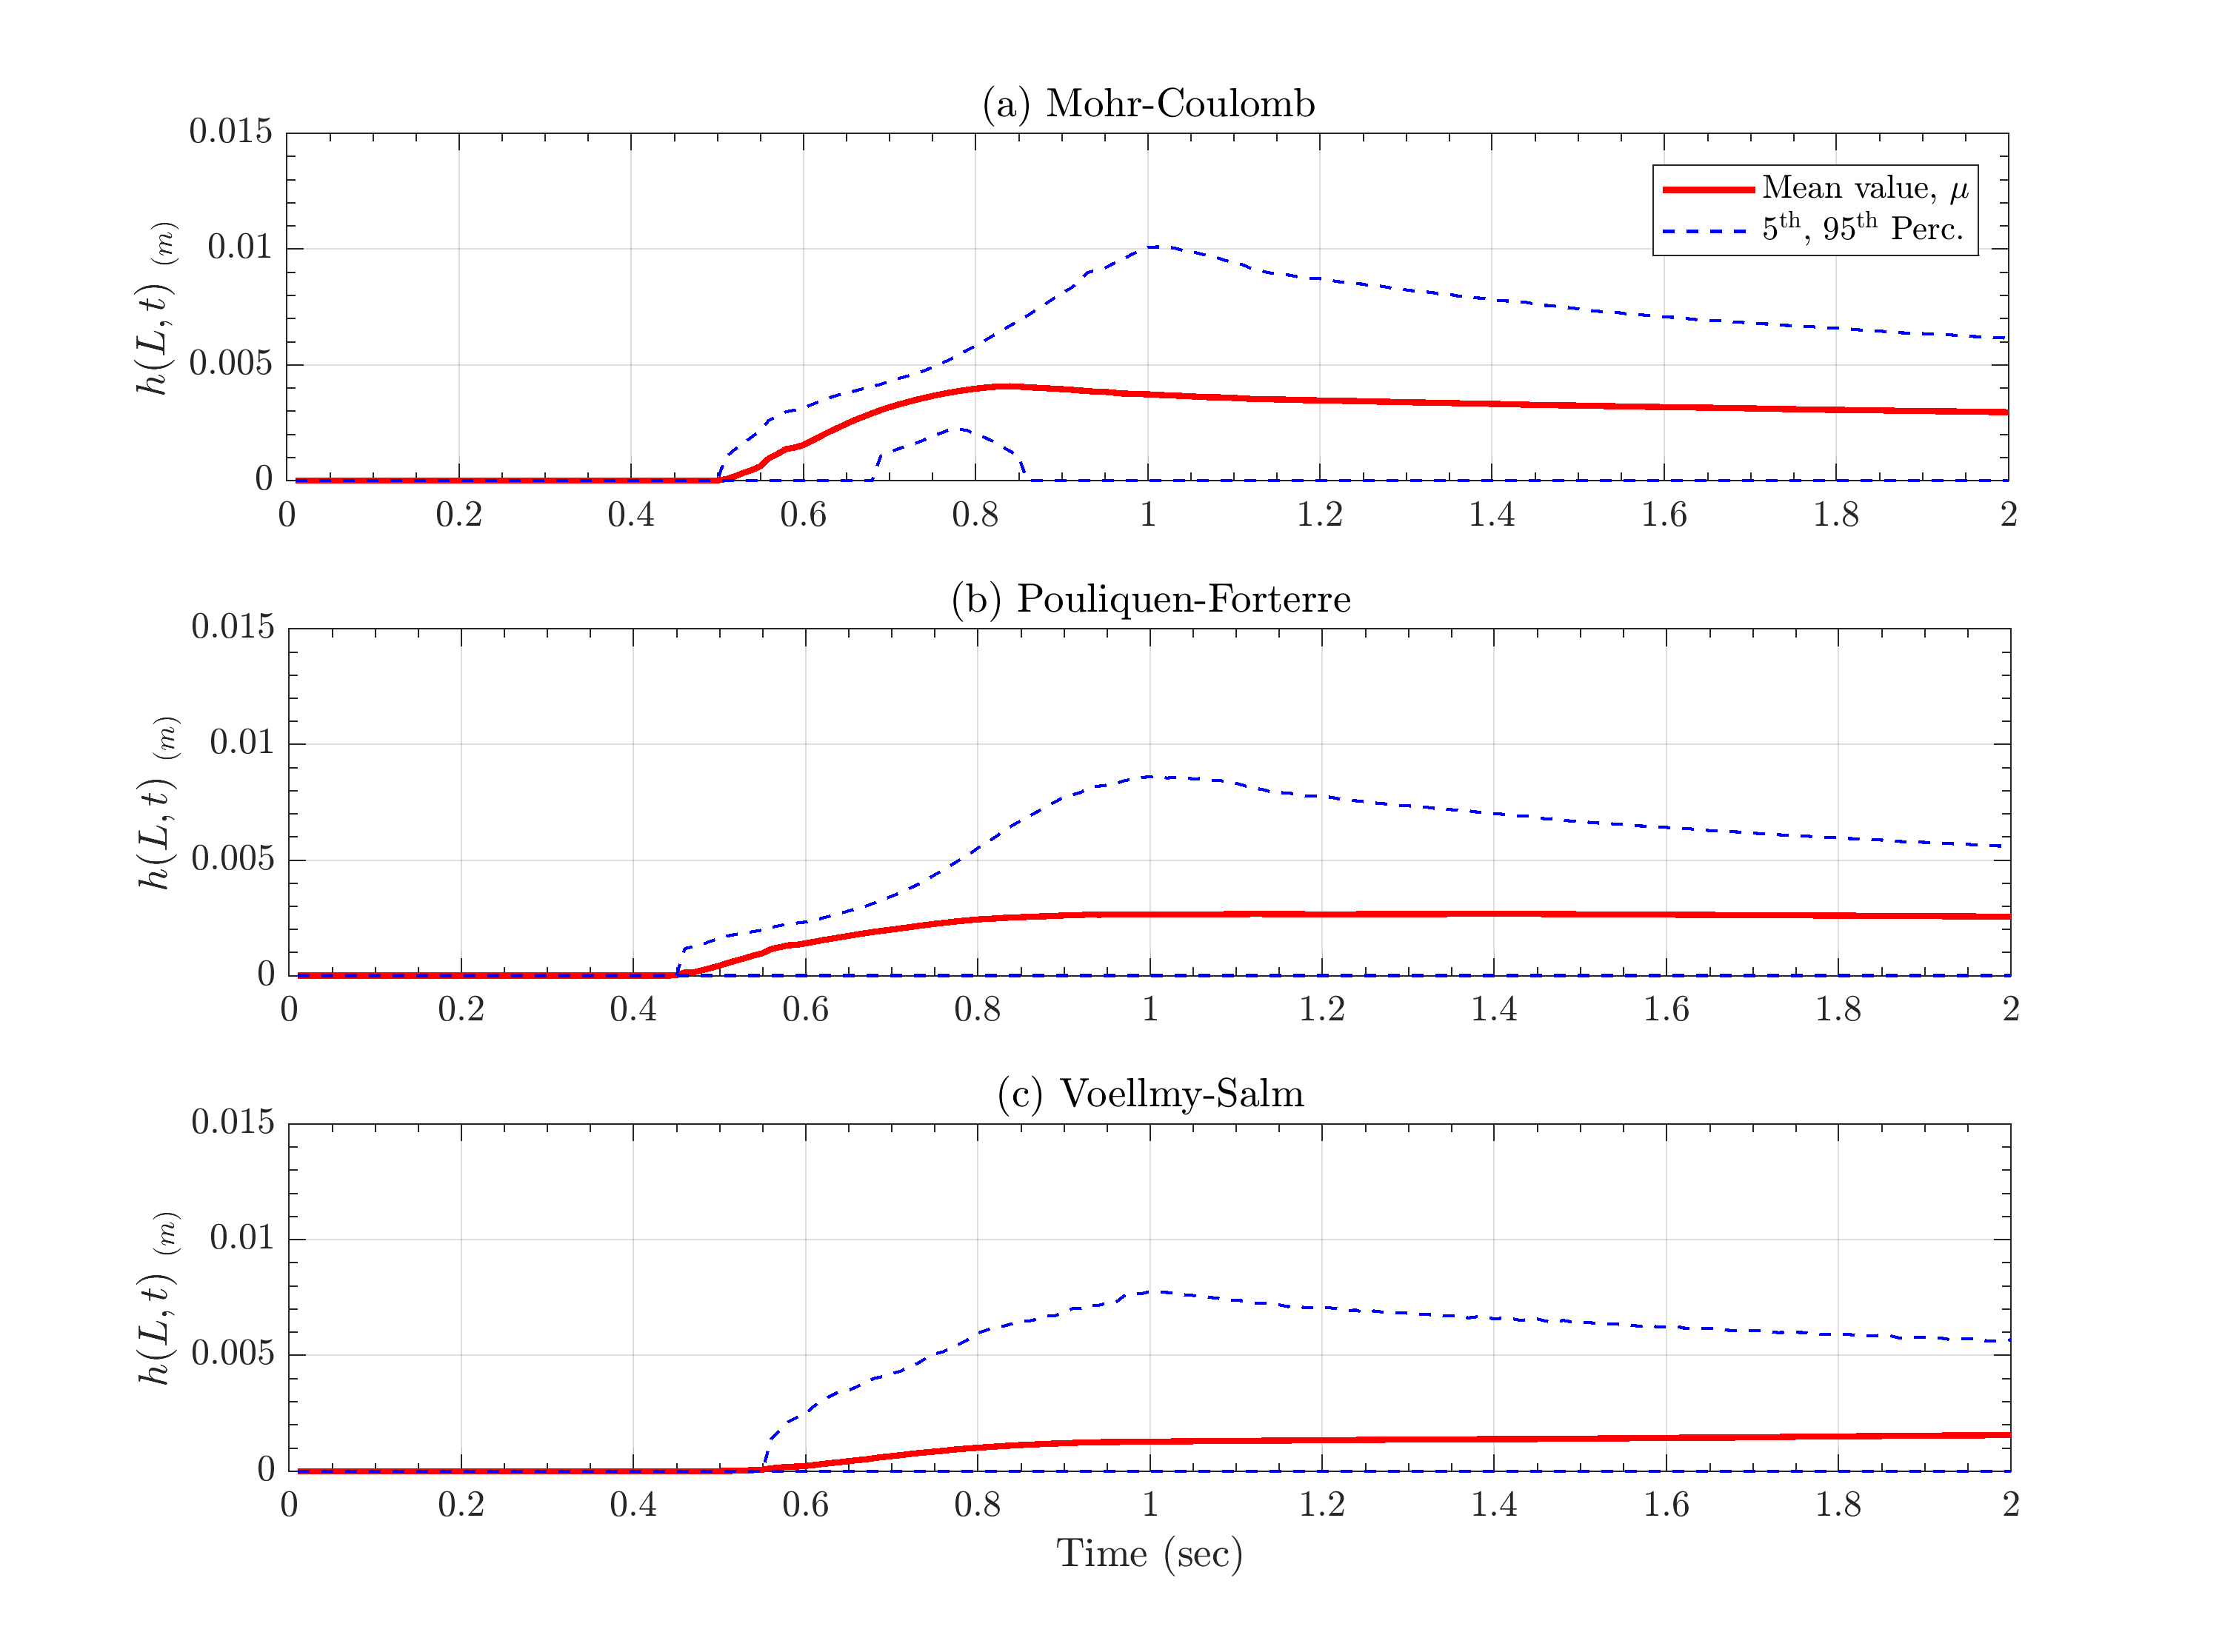
\includegraphics[width=1\textwidth]{InclinedPlane/Height/H_L4.png}
    	\subcaption{$L=(0.15,0)$, a location on runout plane.}
    	\label{fig:Ramp-L4-H}
    \end{minipage}
    \caption{Records of flow height, $h(L,t)$.}
    \label{fig:Ramp-LM-H}
\end{figure}

\begin{figure}[H]
        \centering
        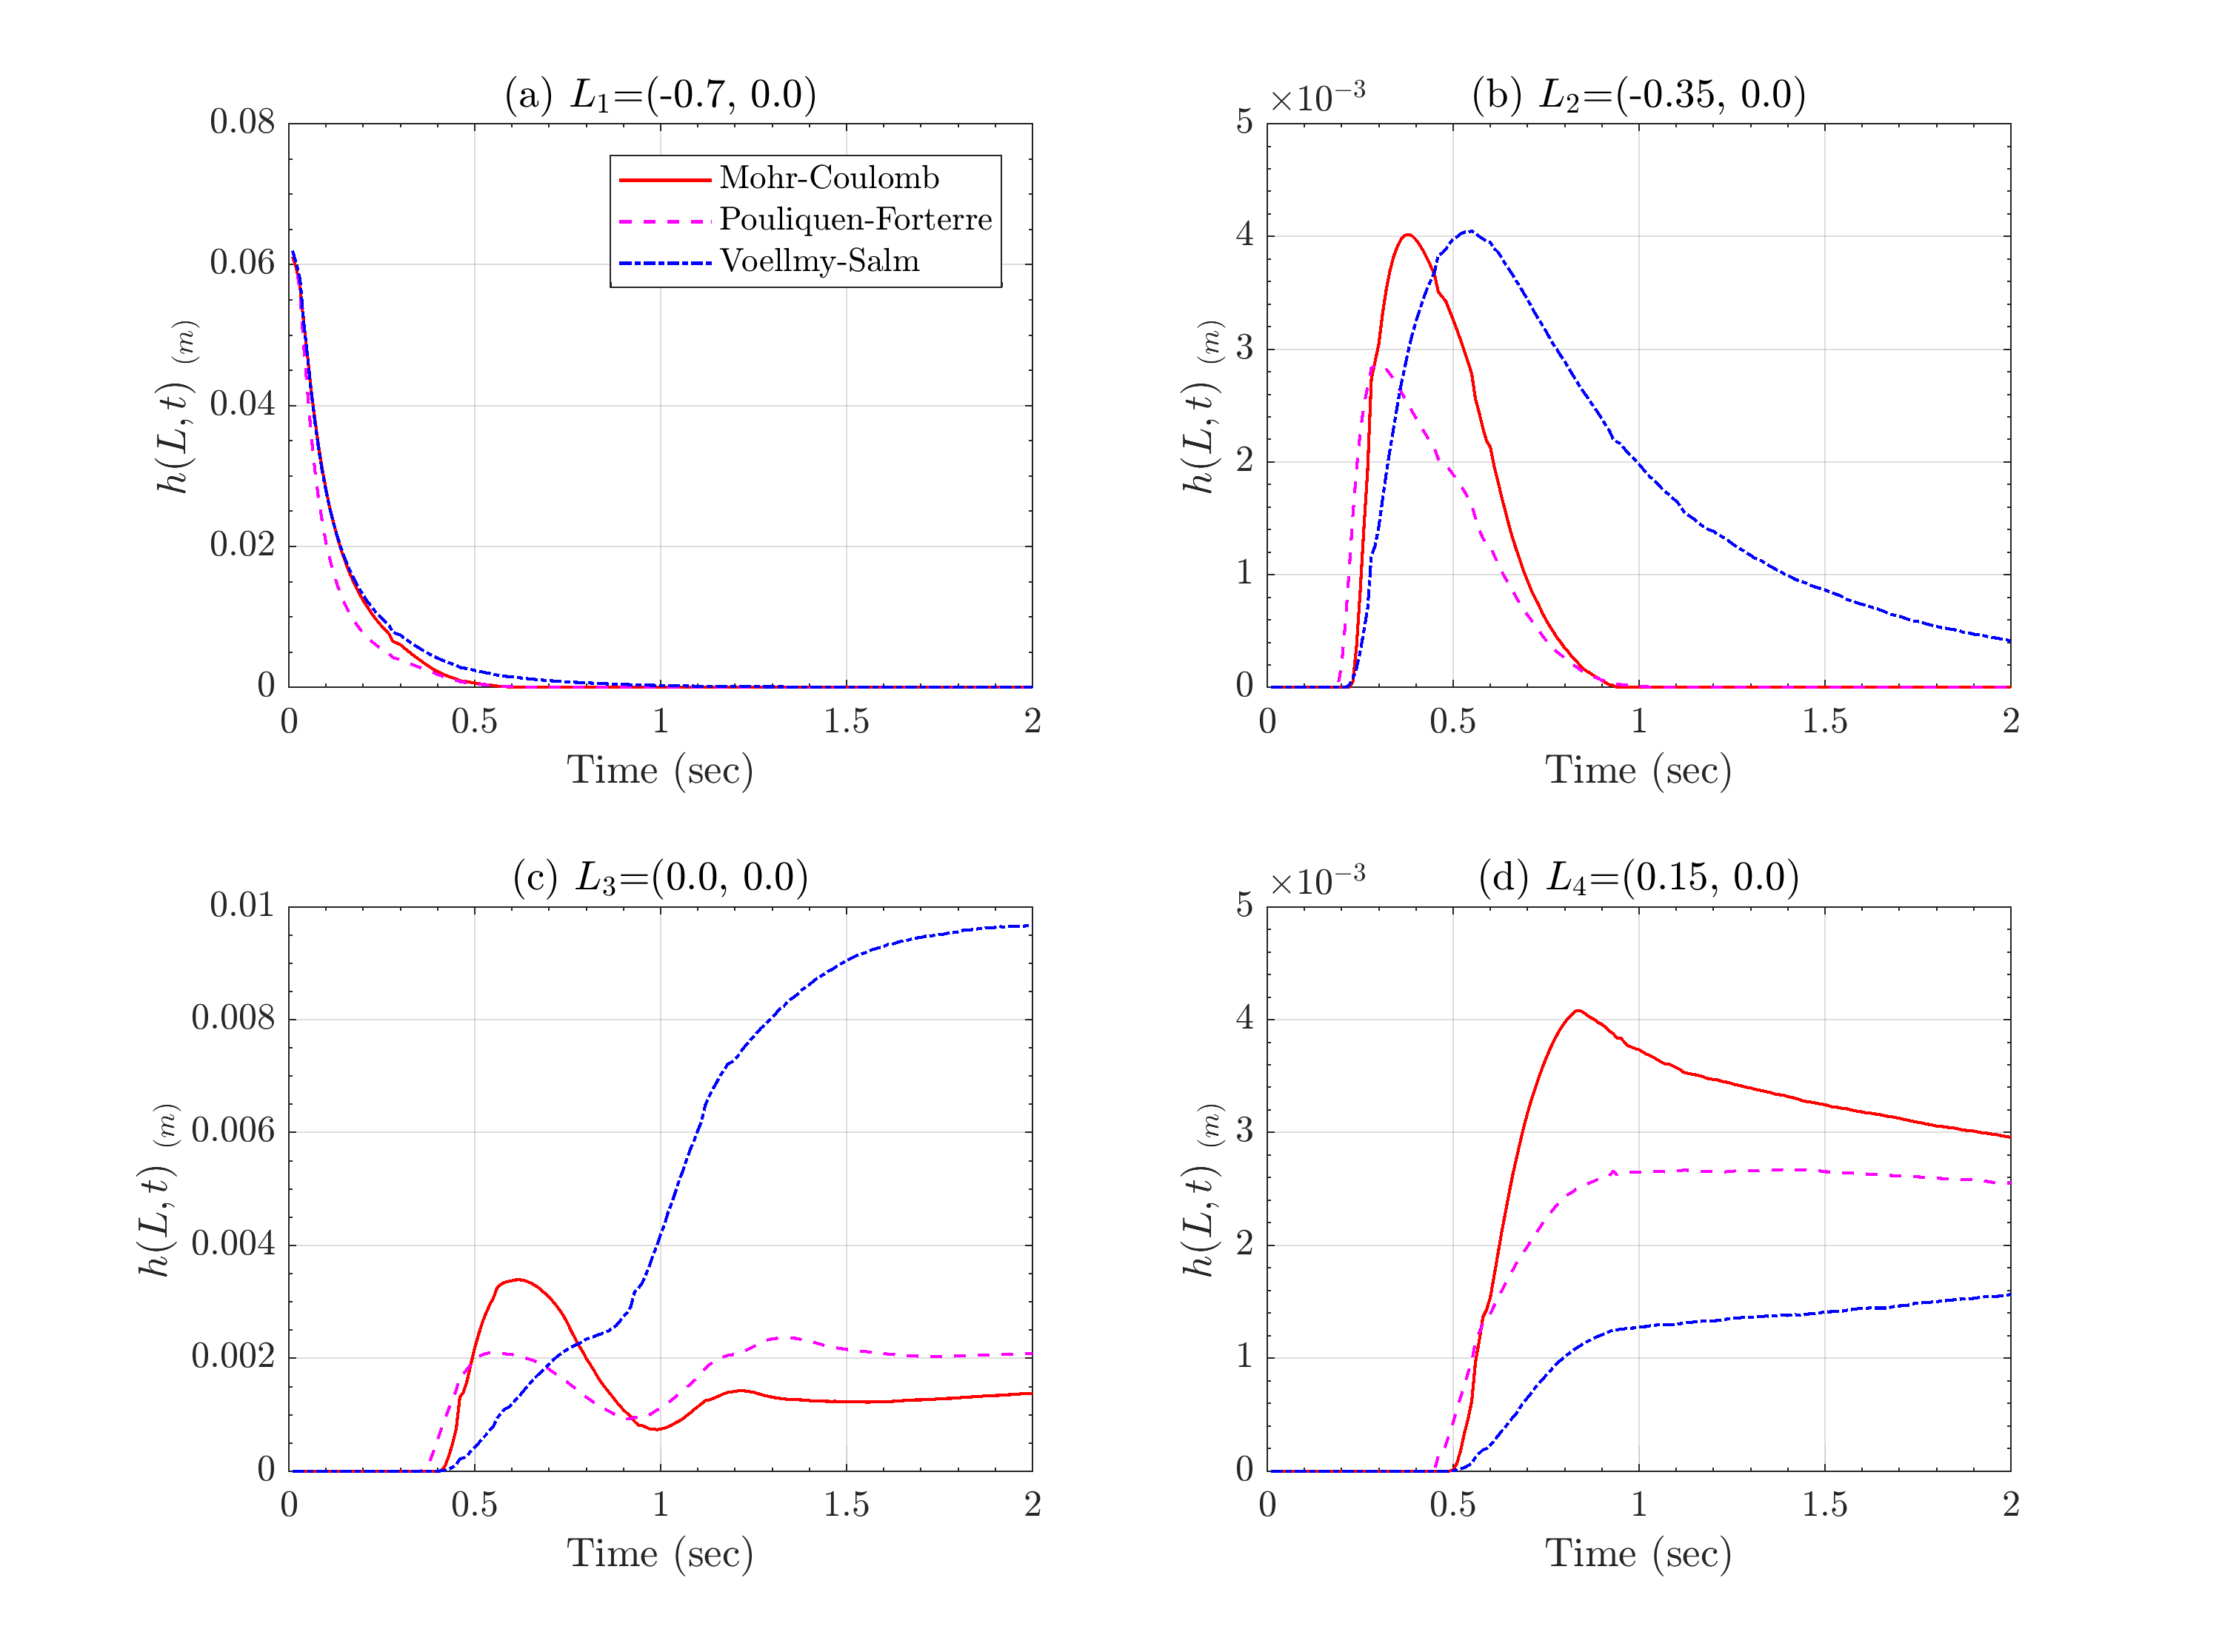
\includegraphics[width=1\textwidth]{InclinedPlane/Height/H_mean.png}
        \caption{Comparison between mean values of flow height, $h(L,t)$, recorded at locations of interest, $L_i, \ _{i=1,...,4}$.}
        \label{fig:Ramp-LM-H-means}
\end{figure}

\begin{figure}[H]
        \centering
        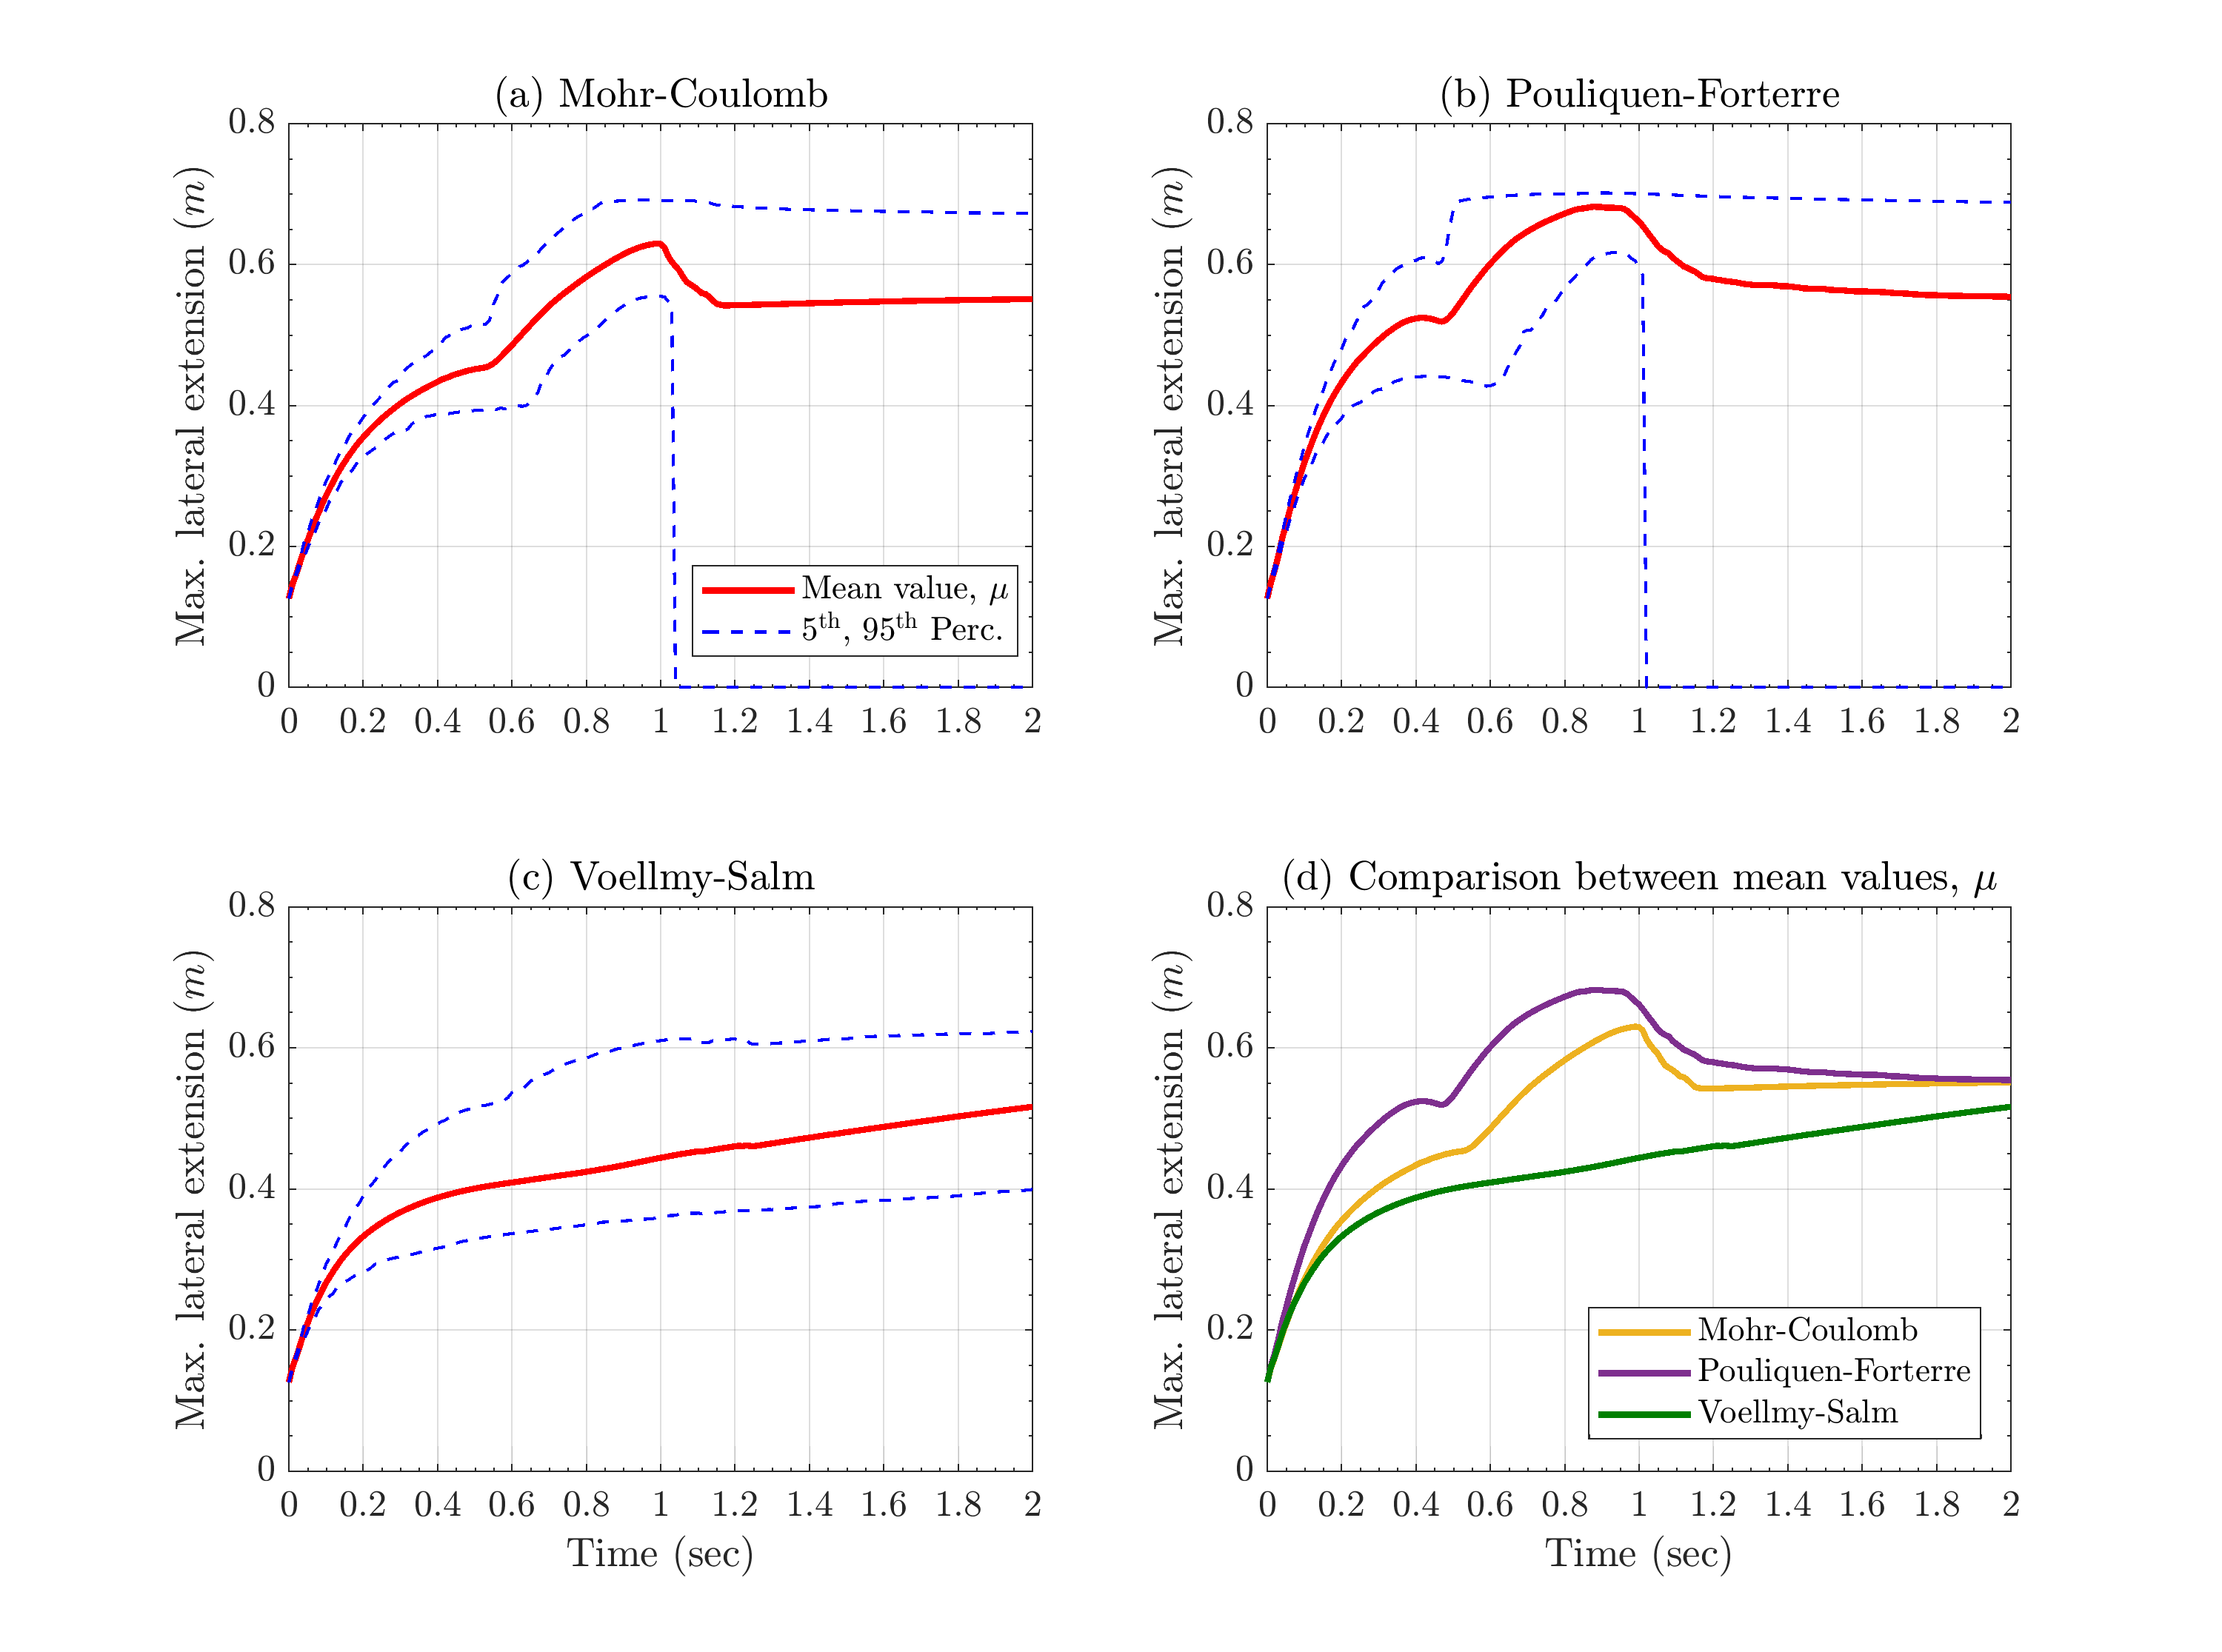
\includegraphics[width=1\textwidth]{InclinedPlane/Height/LateralExtent_SpatialRec.png}
        \caption{Comparison between mean values of flow height recorded at locations of interest, $L_i, \ _{i=1,...,4}$.}
        \label{fig:Ramp-LatExtension-spatial}
\end{figure}

\begin{figure}[H]
        \centering
        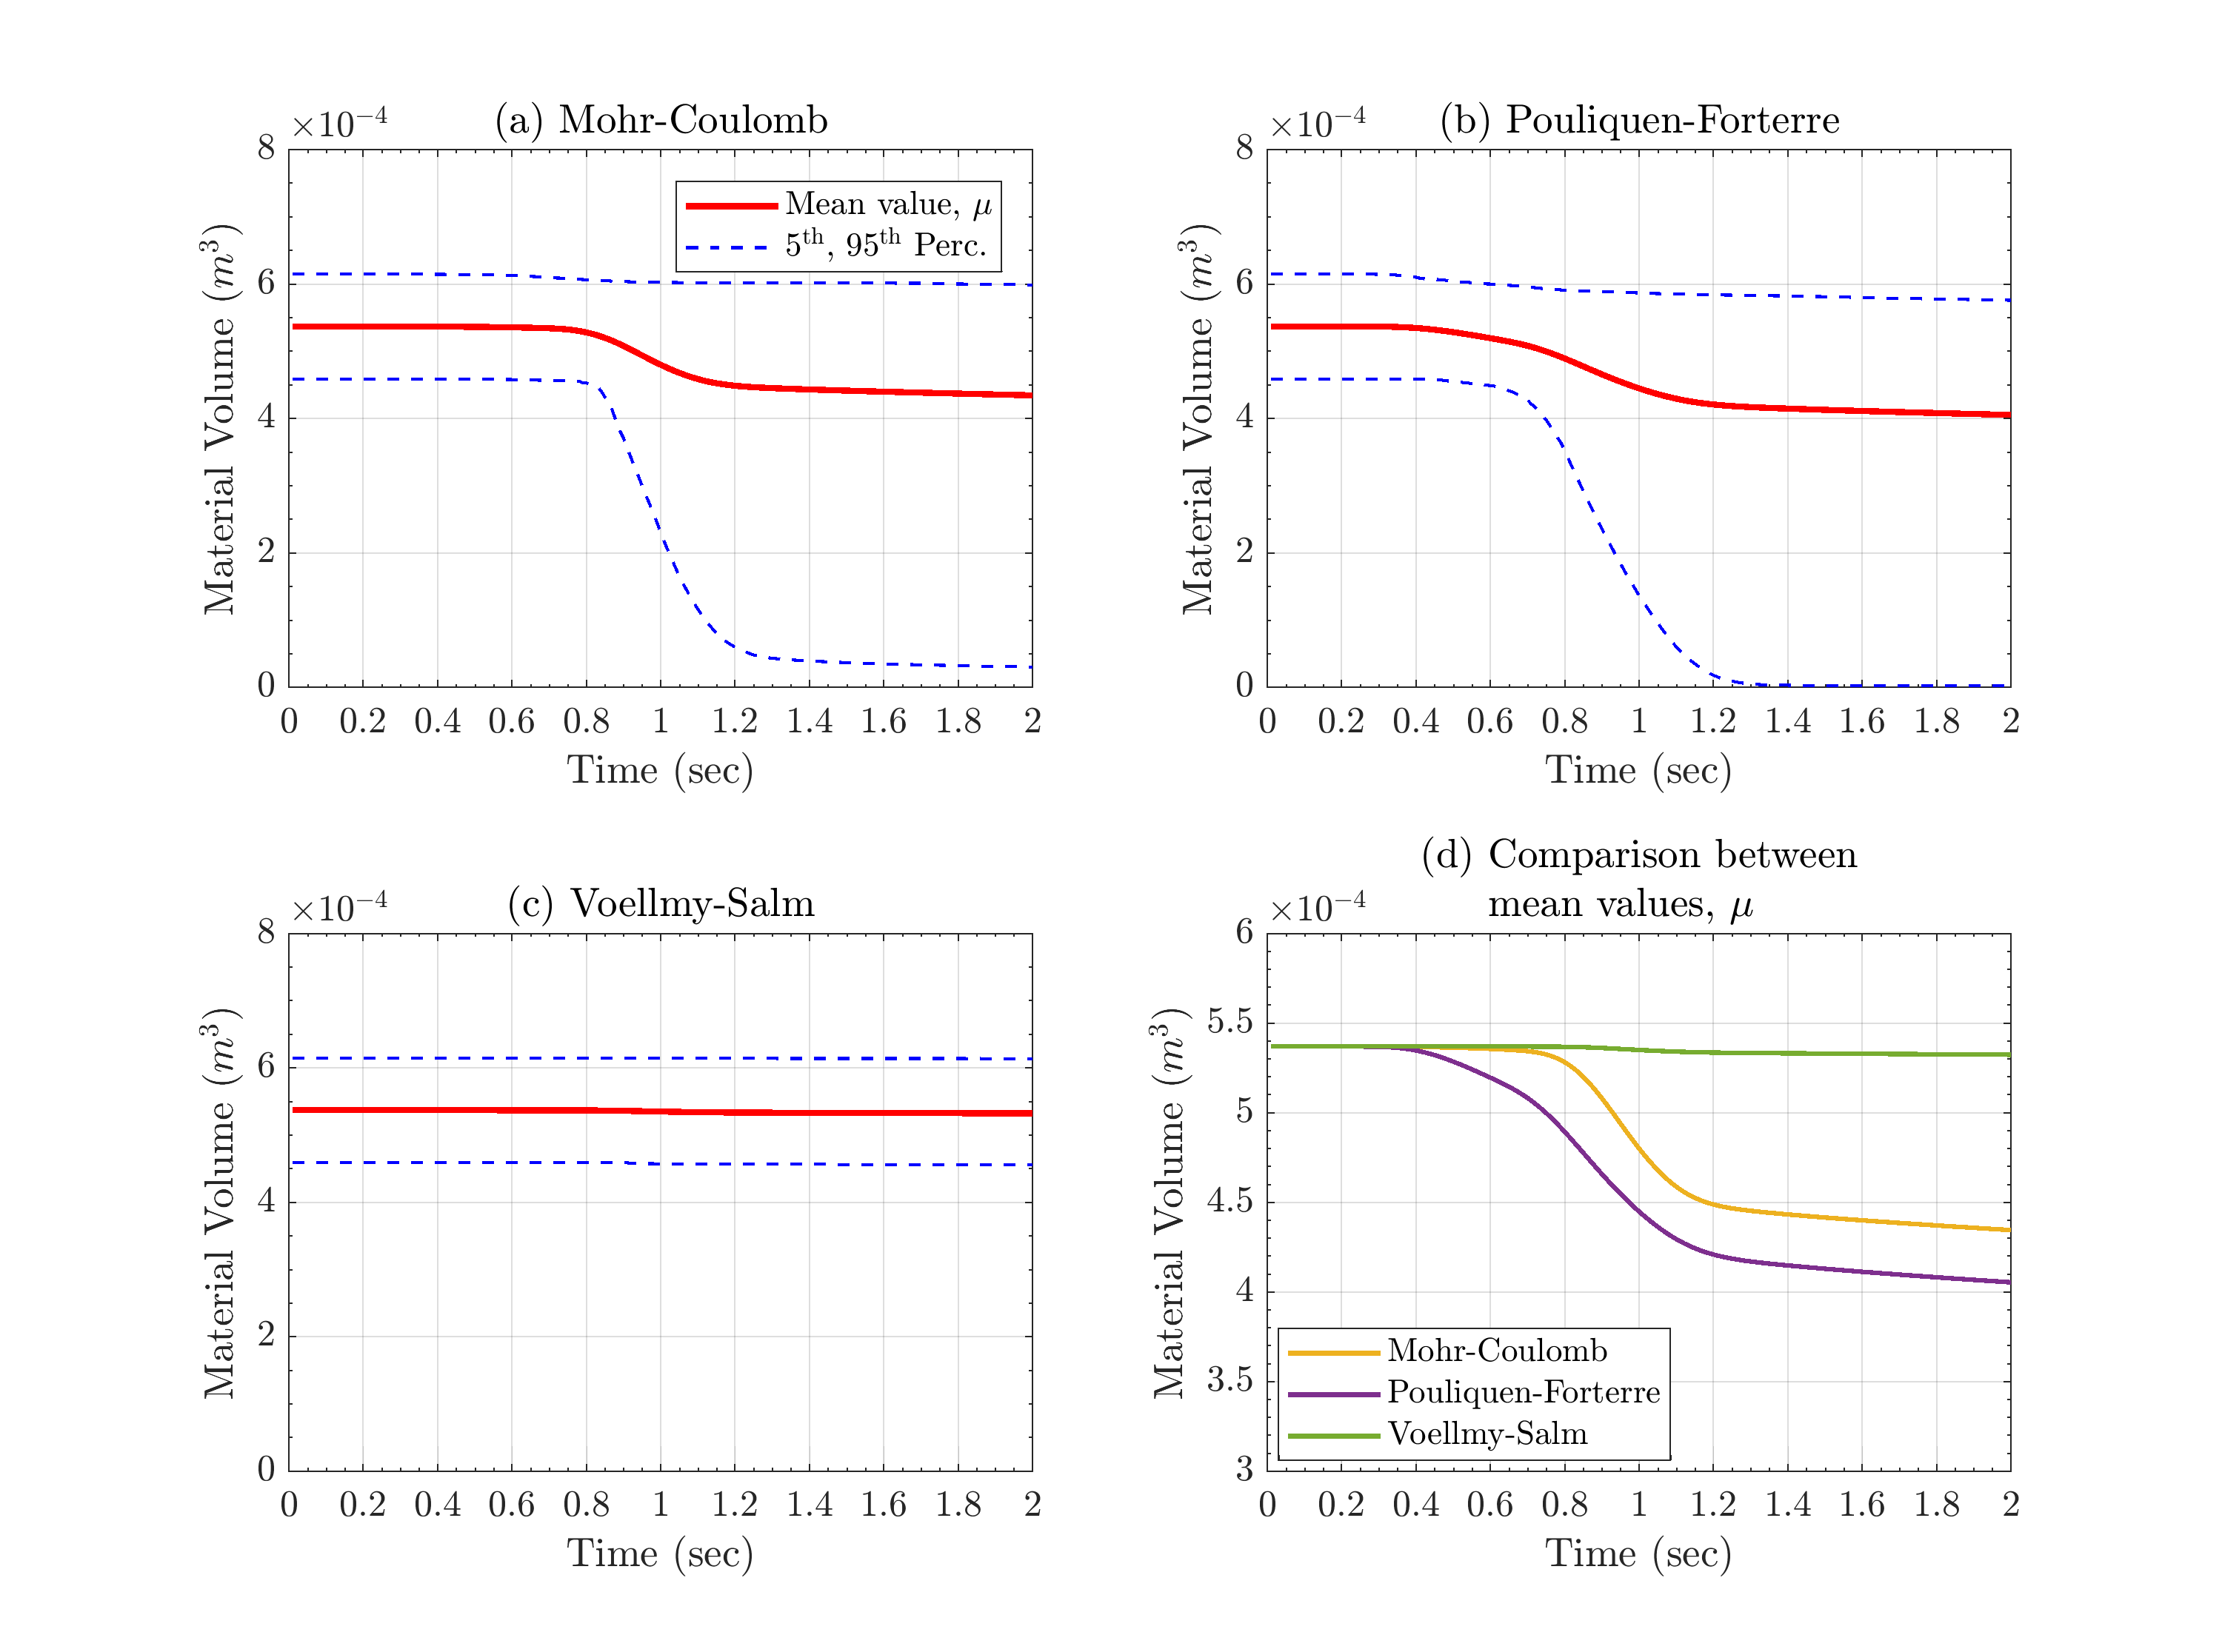
\includegraphics[width=1\textwidth]{InclinedPlane/Height/Volume_SpatialRec.png}
        \caption{Comparison between mean values of flow height, $h(L,t)$, recorded at locations of interest, $L_i, \ _{i=1,...,4}$.}
        \label{fig:Ramp-Volume-spatial}
\end{figure}

\begin{figure}[H]
        \centering
        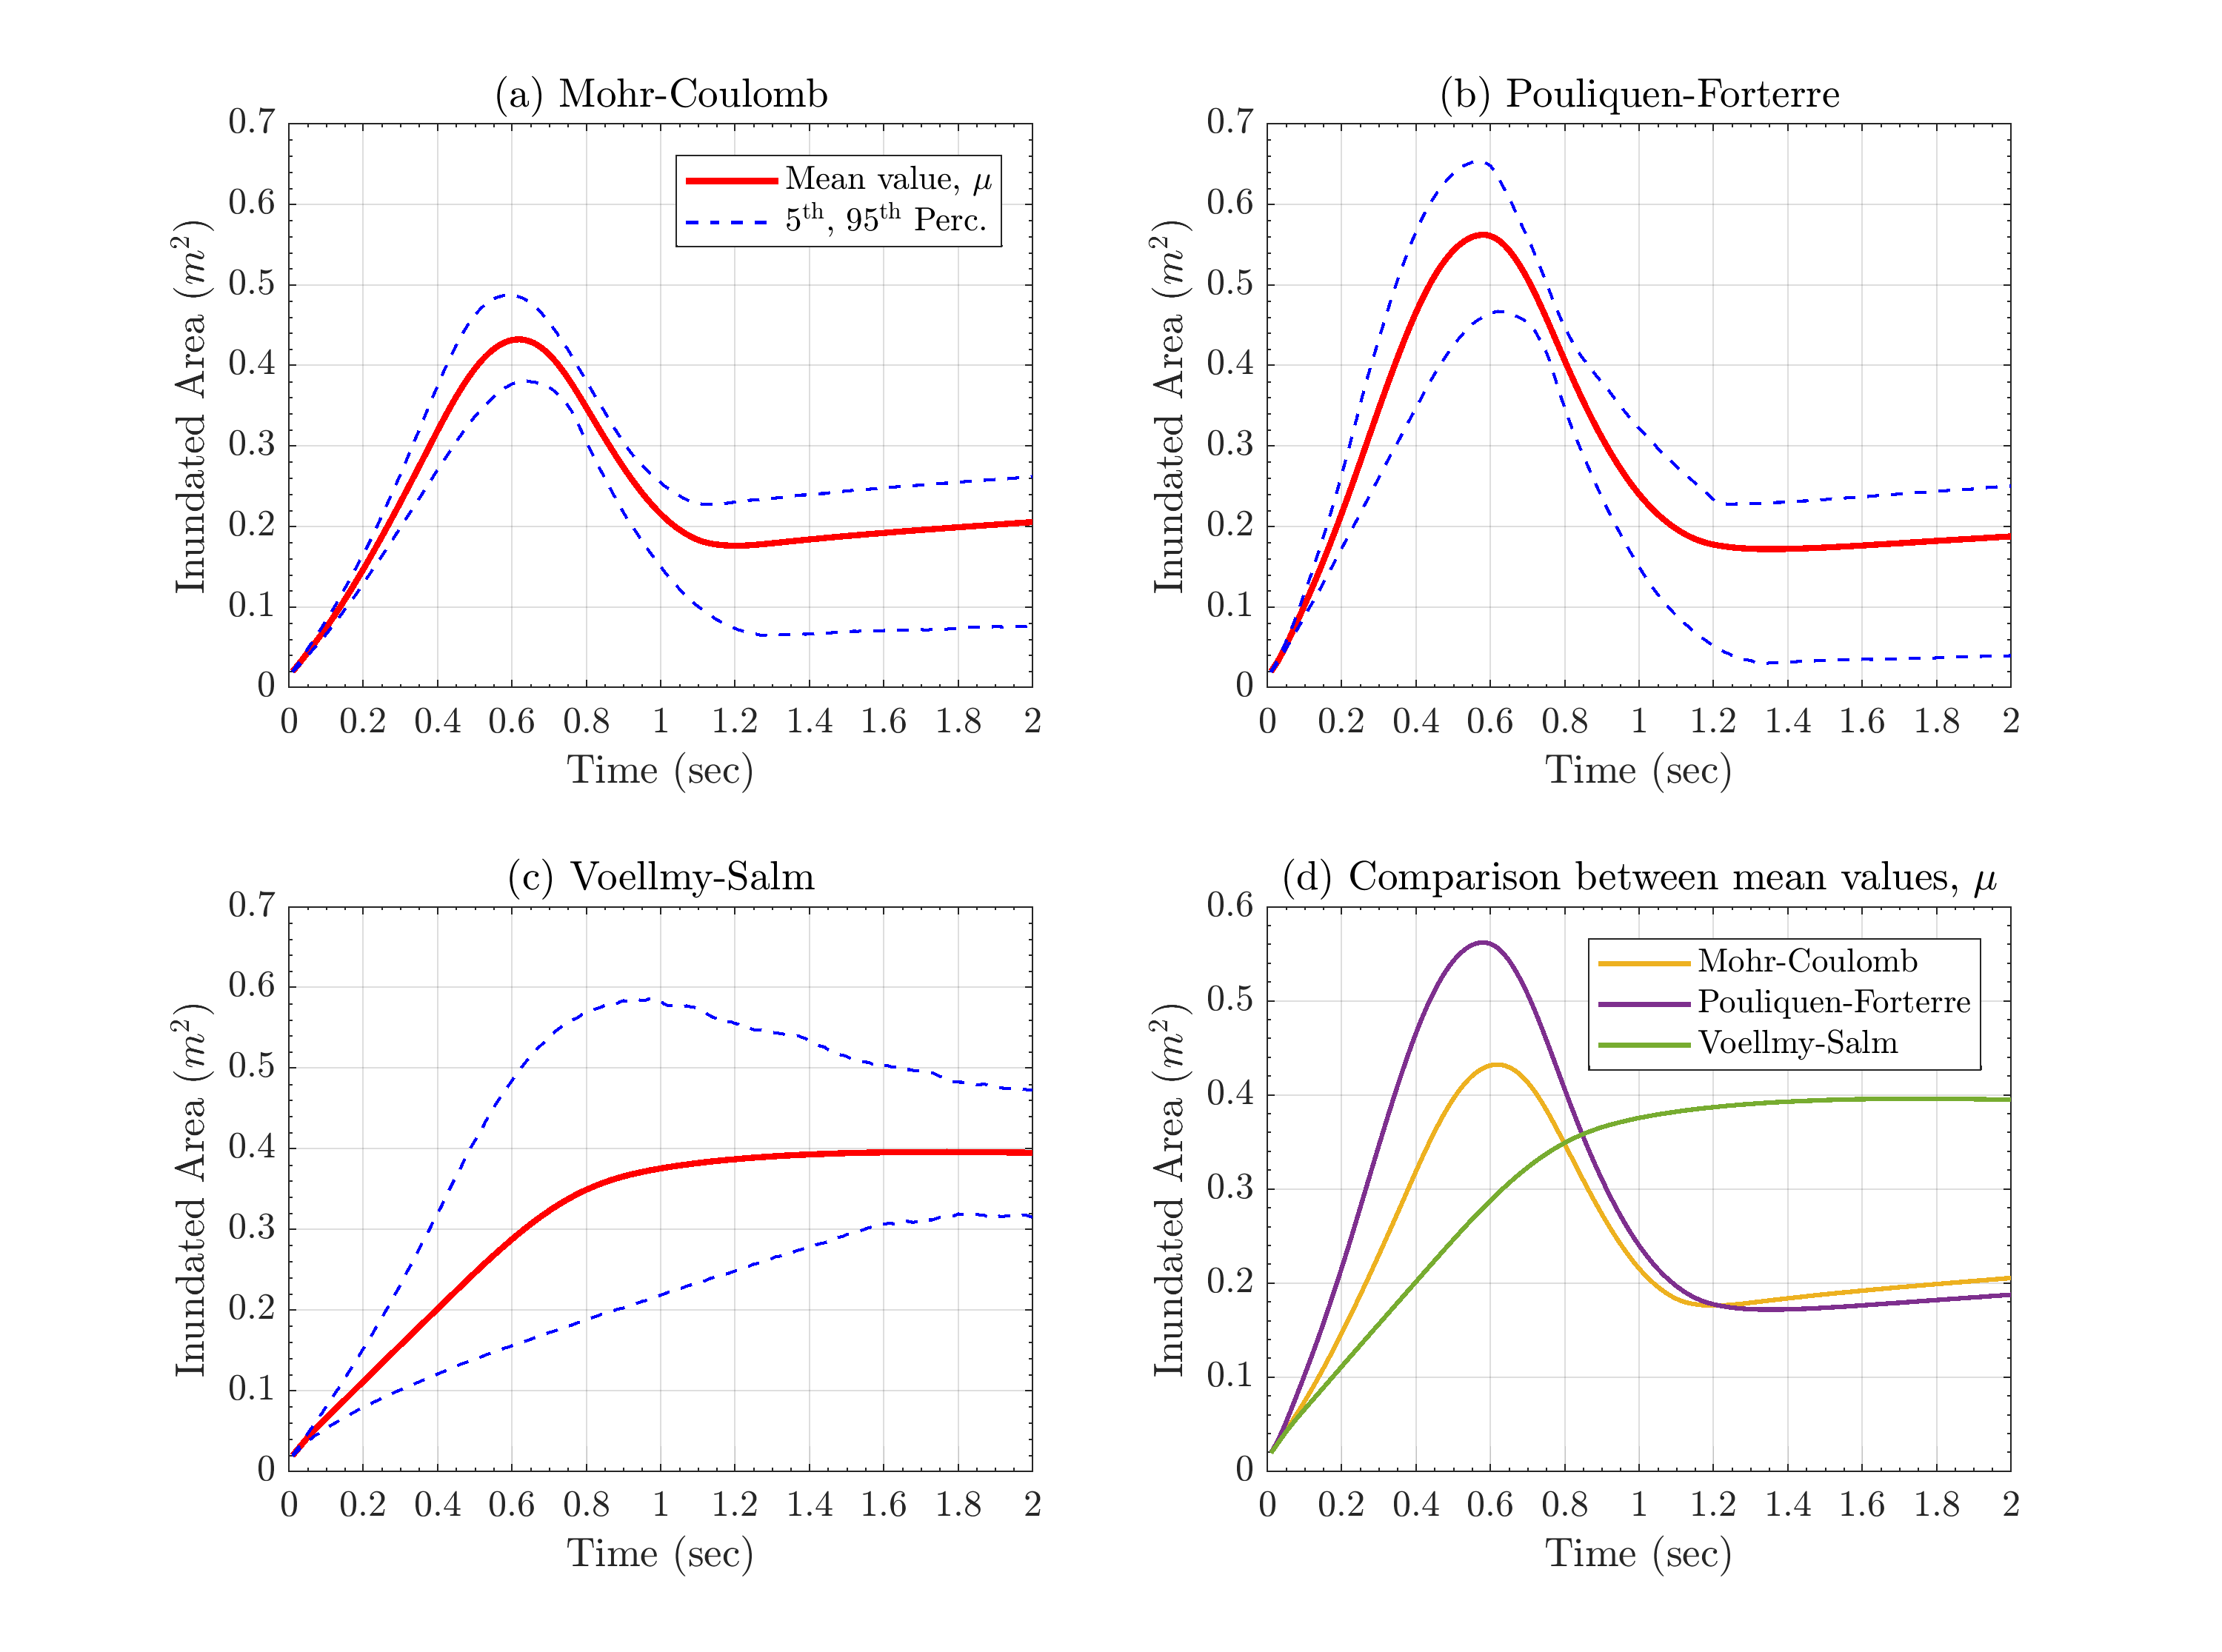
\includegraphics[width=1\textwidth]{InclinedPlane/Height/Area_SpatialRec.png}
        \caption{Comparison between mean values of flow height, $h(L,t)$, recorded at locations of interest, $L_i, \ _{i=1,...,4}$.}
        \label{fig:Ramp-InundArea-spatial}
\end{figure}

\subsubsection{Flow Velocity}
\begin{figure}[H]
	\begin{minipage}[b]{0.5\linewidth}
    	\centering
    	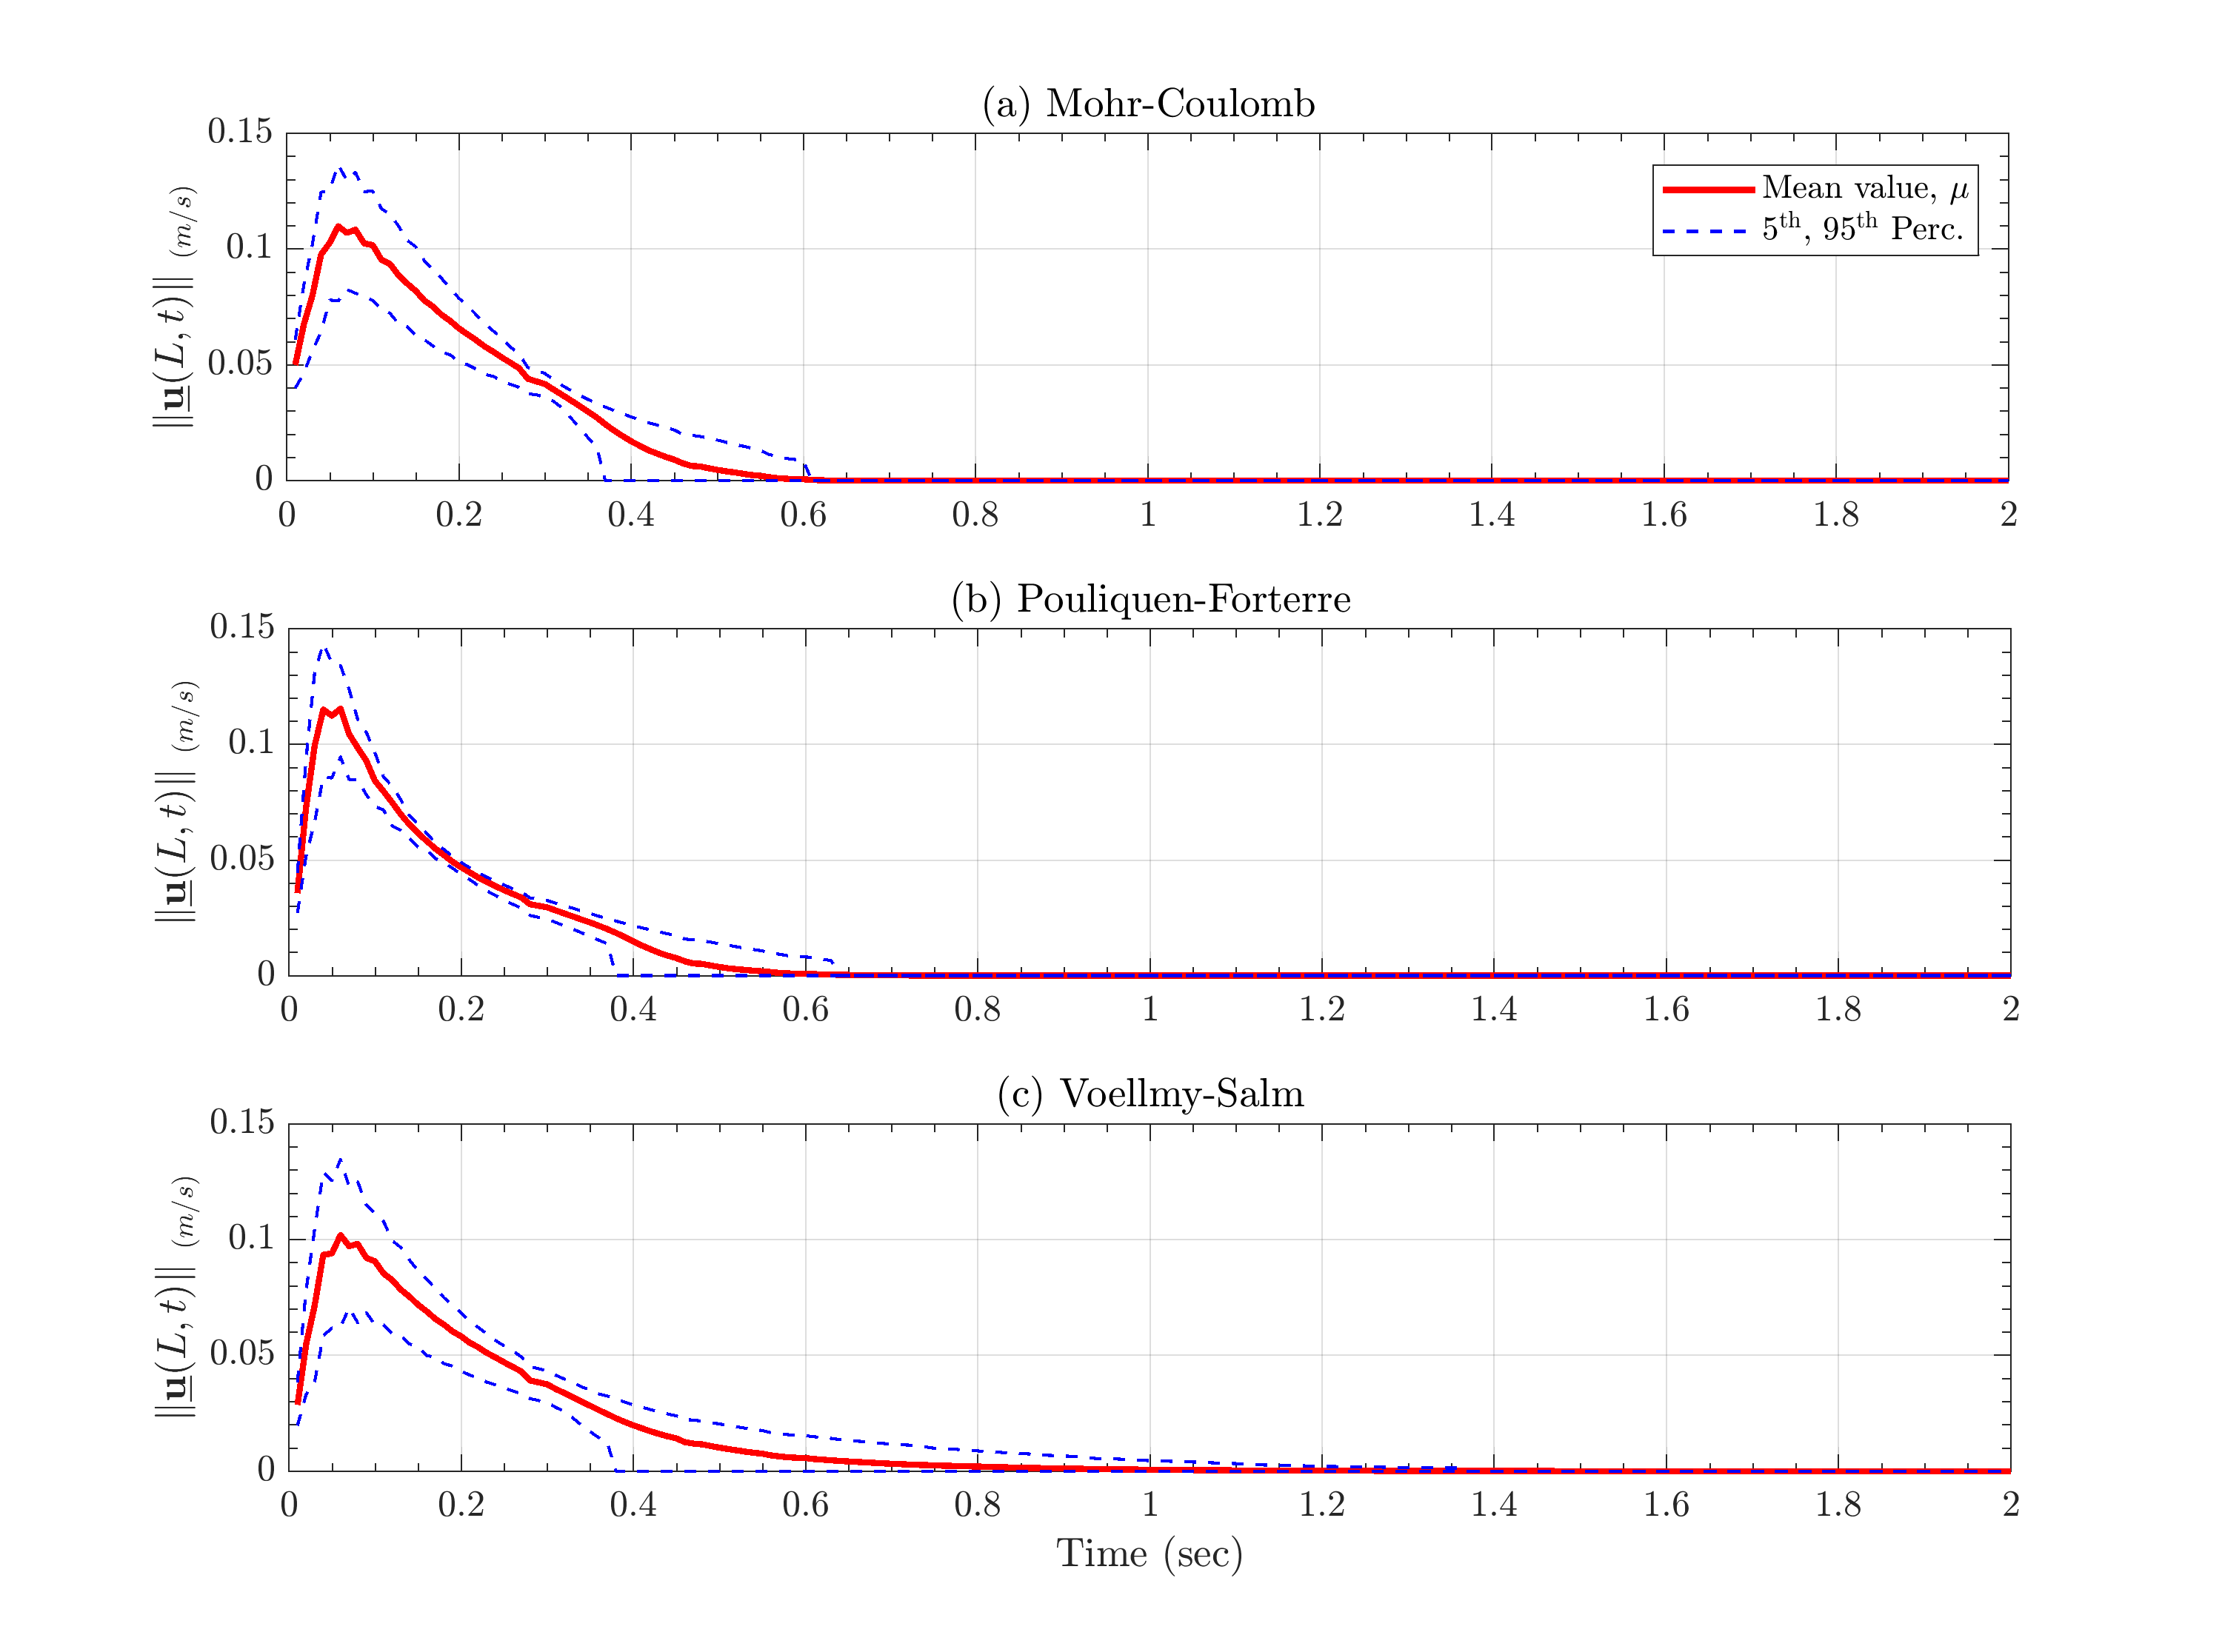
\includegraphics[width=1\textwidth]{InclinedPlane/Velocity/Vel_L1.png}
    	\subcaption{$L=(-0.7,0)$, slumping pile location.}
    	\label{fig:Ramp-L1-Vel}
	\end{minipage}
	\begin{minipage}[b]{0.5\linewidth}
		\centering
		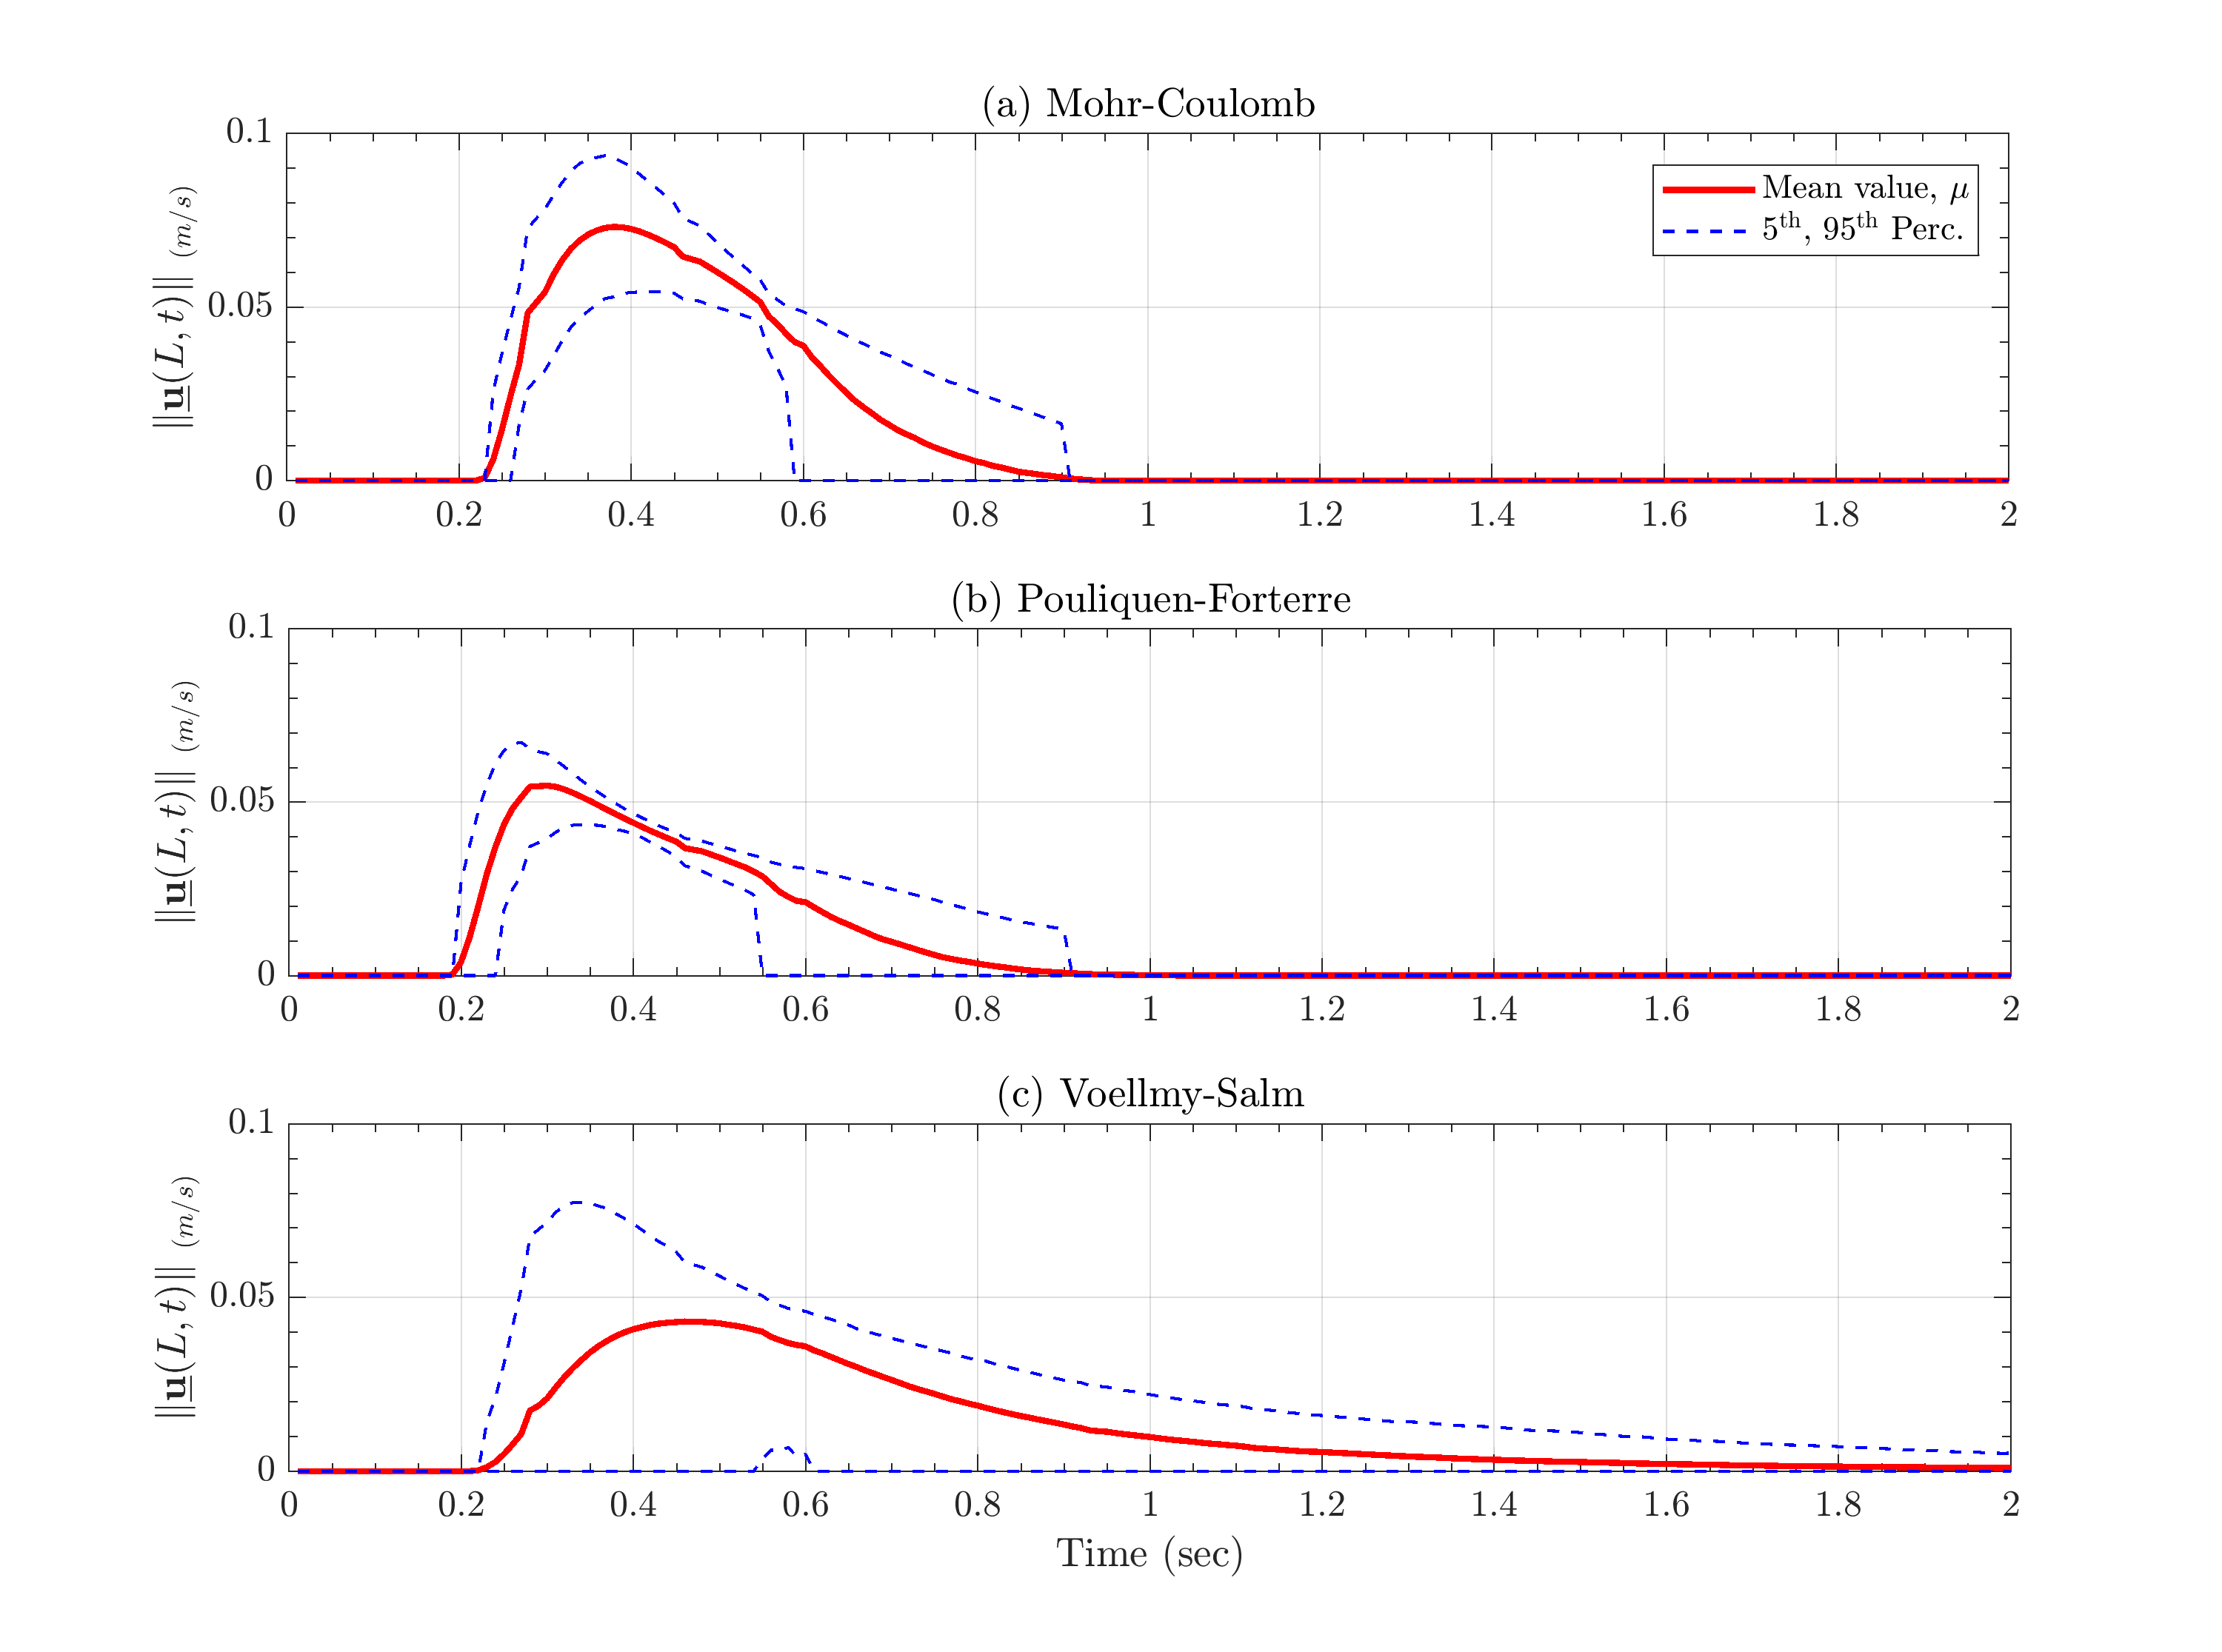
\includegraphics[width=1\textwidth]{InclinedPlane/Velocity/Vel_L2.png}
    	\subcaption{$L=(-0.35,0)$, middle point on inclined plane.}
    	\label{fig:Ramp-L2-Vel}
    \end{minipage}

	\begin{minipage}[b]{0.5\linewidth}
    	\centering
    	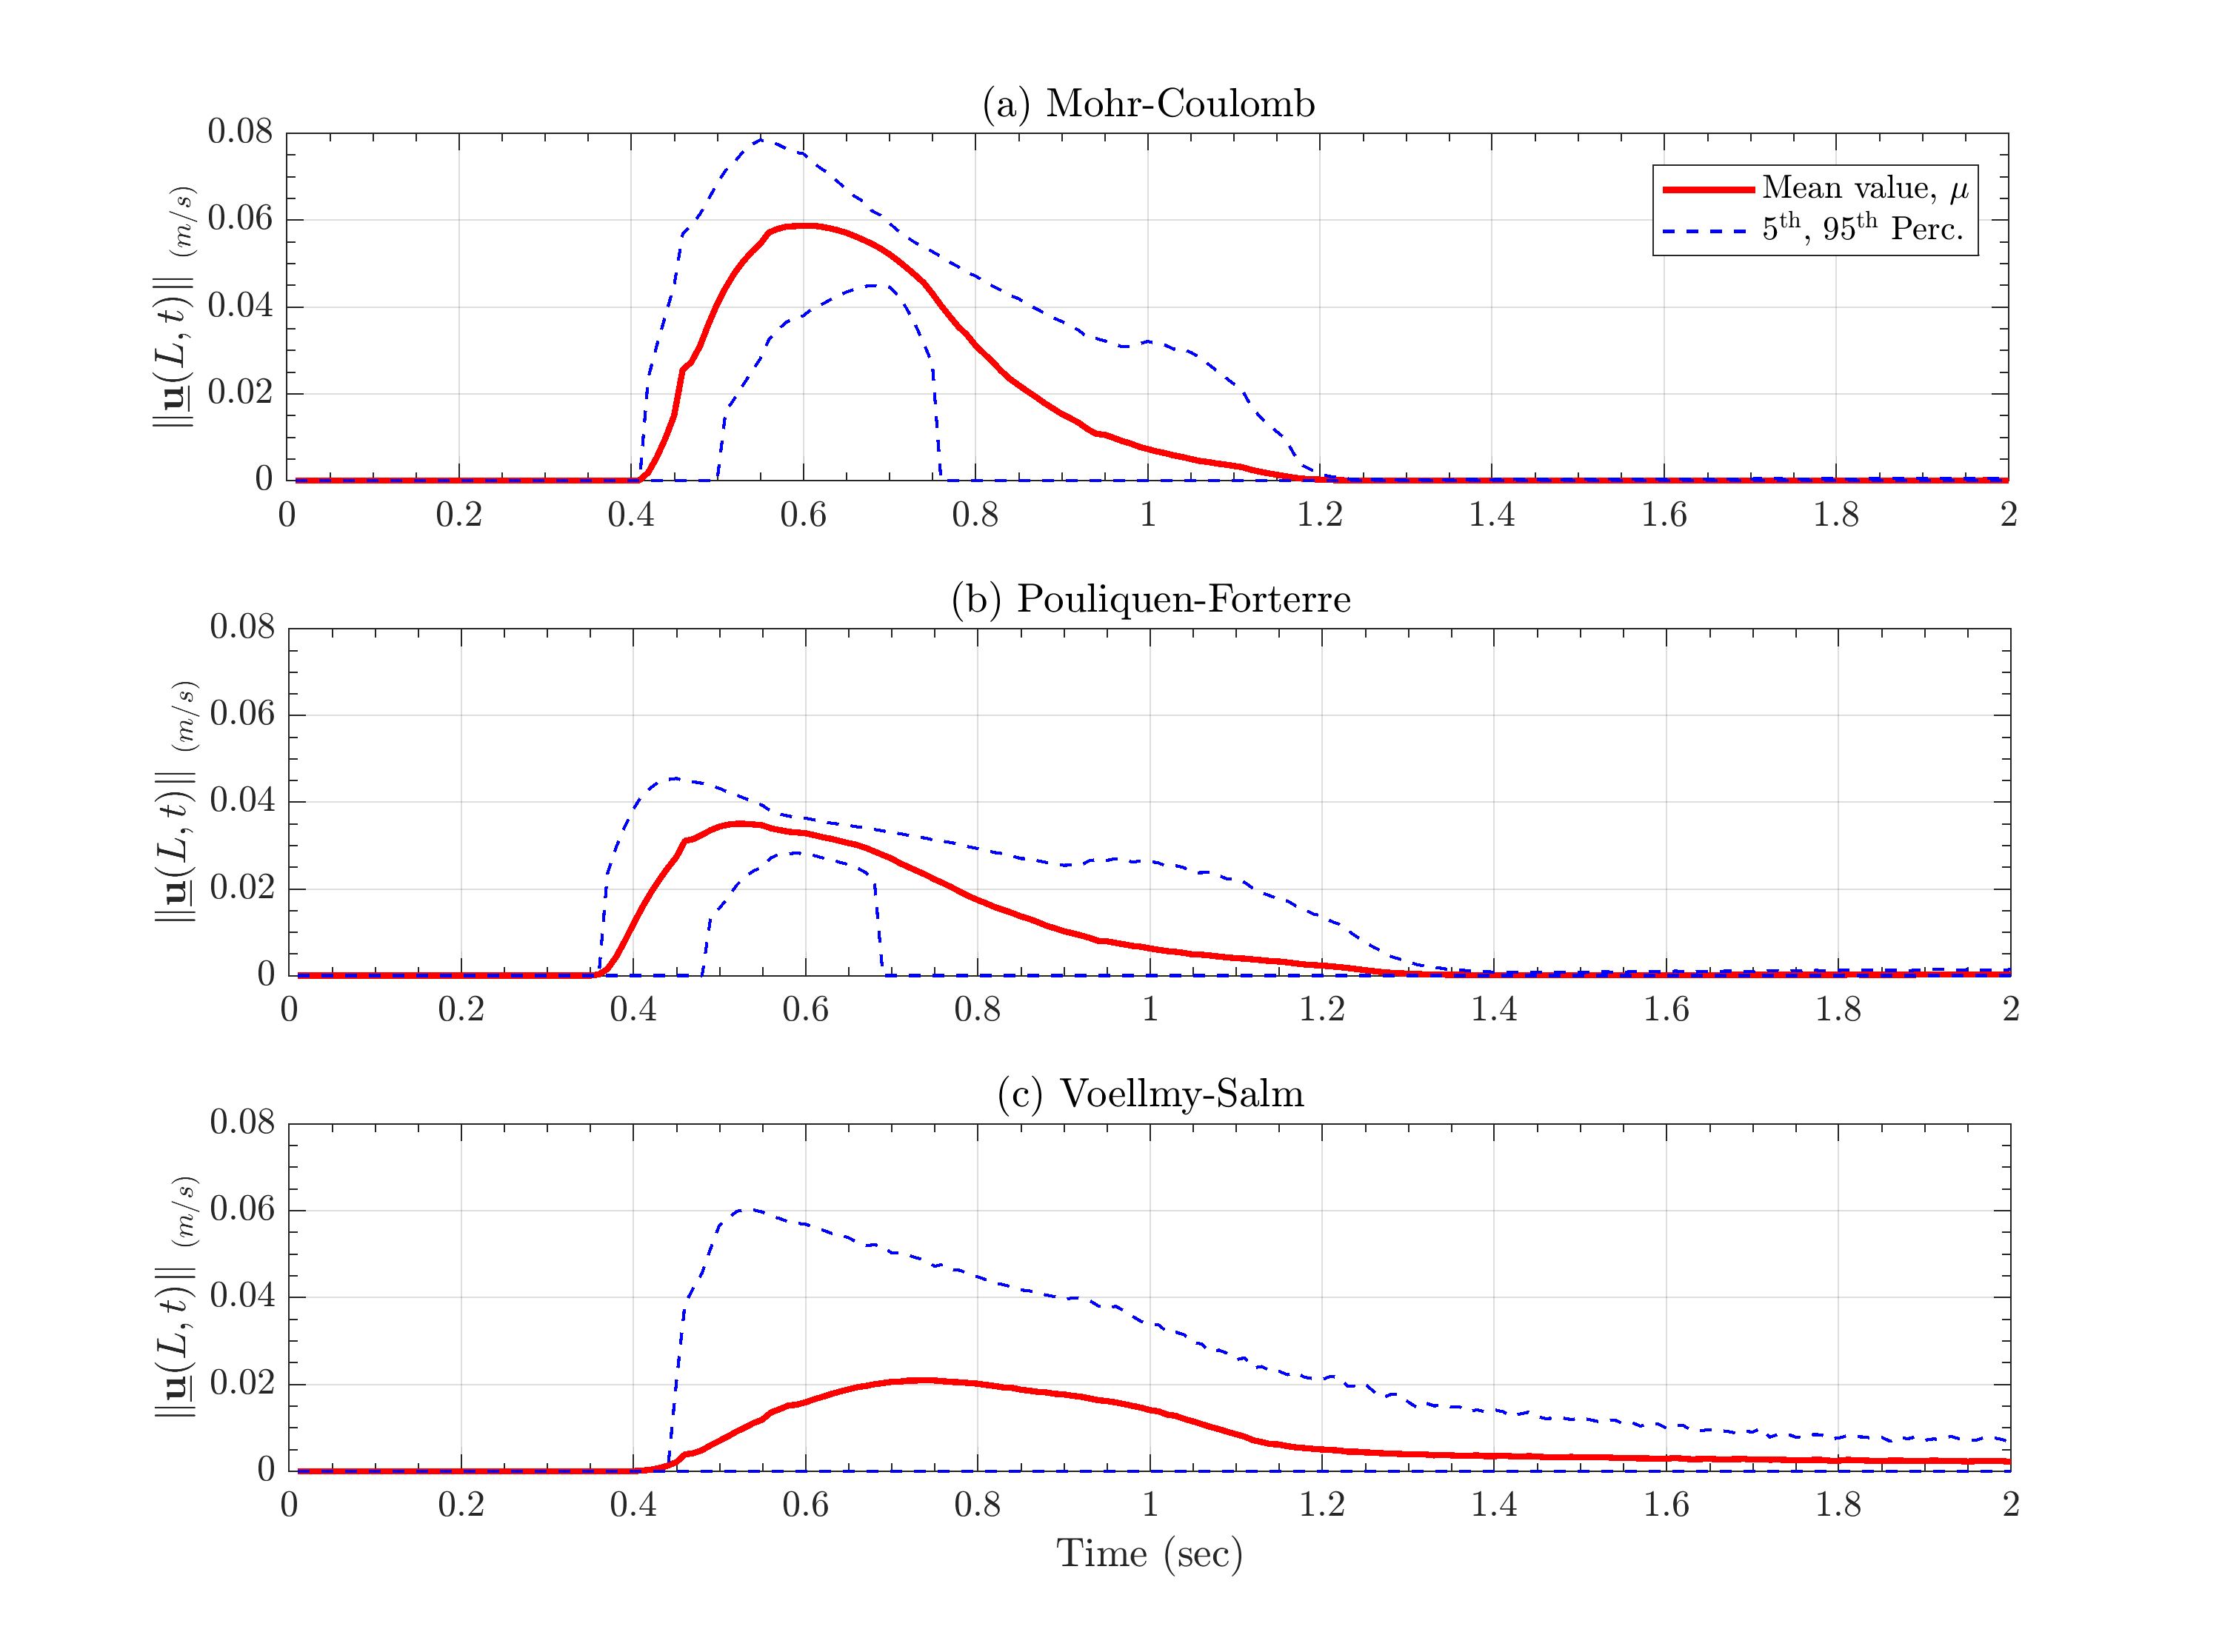
\includegraphics[width=1\textwidth]{InclinedPlane/Velocity/Vel_L3.png}
    	\subcaption{$L=(0,0)$, inclined and runout planes' joint location.}
    	\label{fig:Ramp-L3-Vel}
	\end{minipage}
	\begin{minipage}[b]{0.5\linewidth}
		\centering
		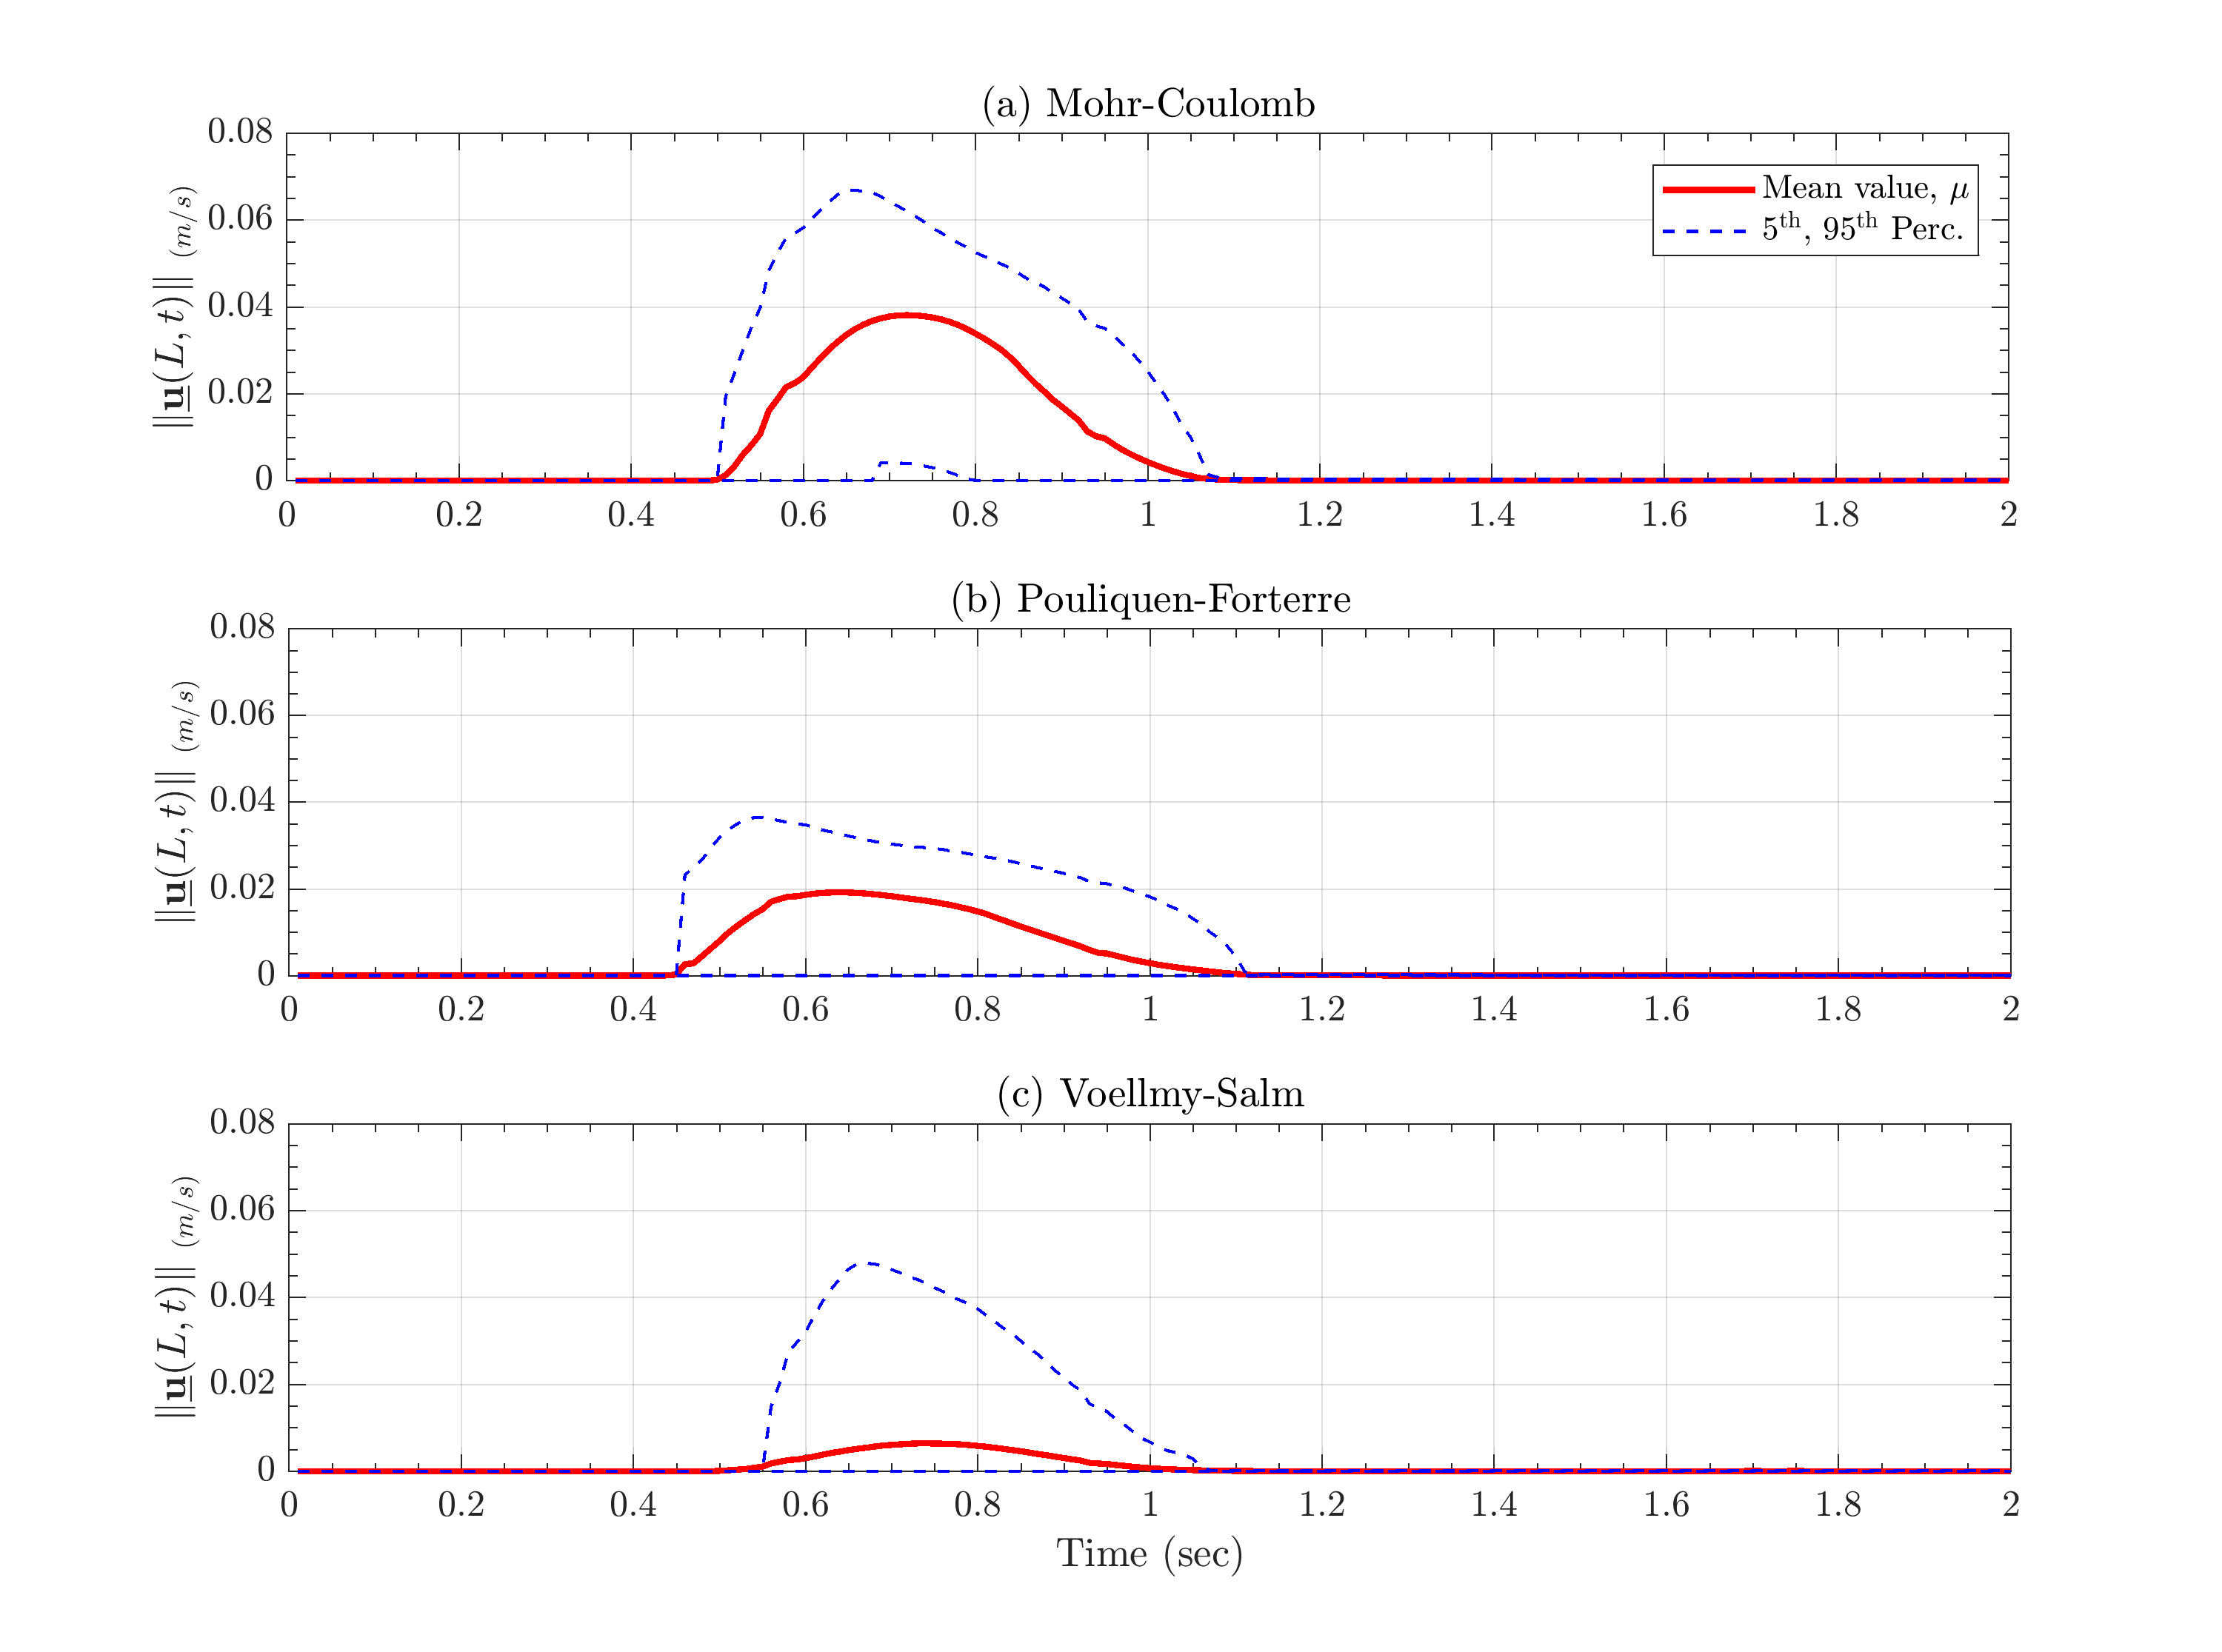
\includegraphics[width=1\textwidth]{InclinedPlane/Velocity/Vel_L4.png}
    	\subcaption{$L=(0.15,0)$, a location on runout plane.}
    	\label{fig:Ramp-L4-Vel}
    \end{minipage}
    \caption{Records of flow velocity, $\Vert \underline{\mathbf{u}} \Vert(L,t)$.}
    \label{fig:Ramp-LM-Vel}
\end{figure}

\begin{figure}[H]
        \centering
        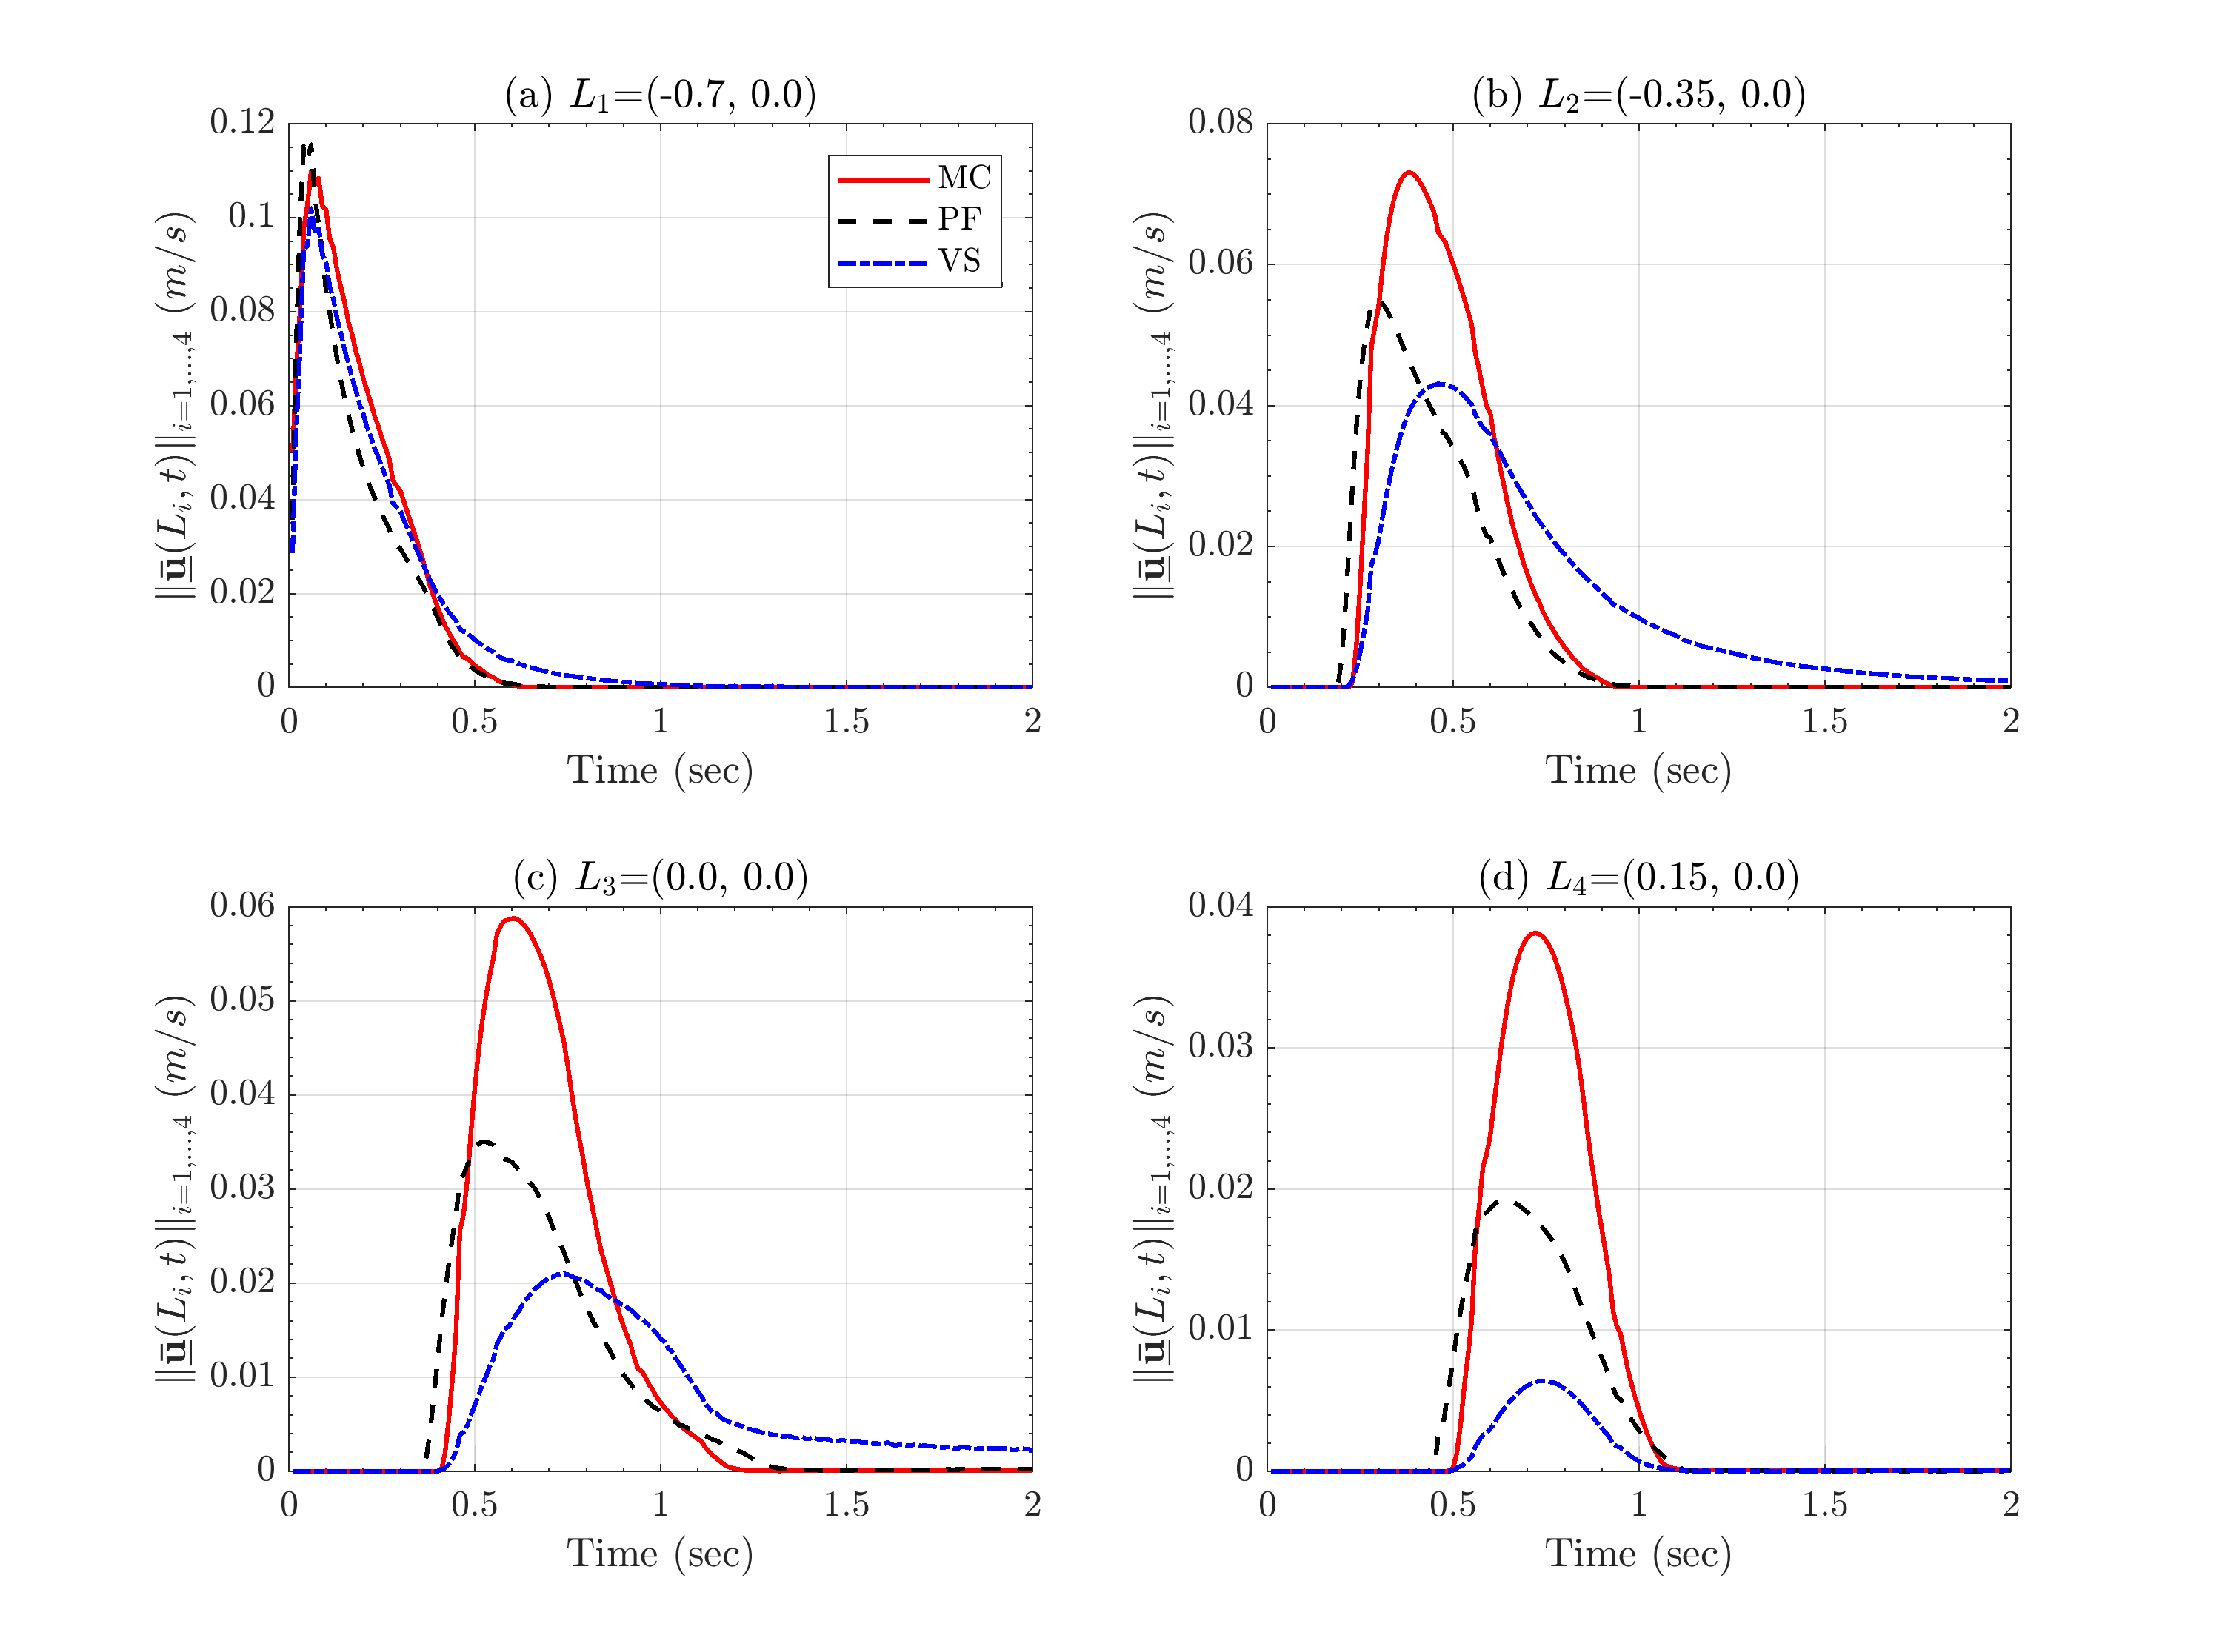
\includegraphics[width=1\textwidth]{InclinedPlane/Velocity/Vel_mean.png}
        \caption{Comparison between mean values of flow velocity, $\Vert \underline{\mathbf{u}} \Vert(L,t)$, recorded at locations of interest, $L_i, \ _{i=1,...,4}$.}
        \label{fig:Ramp-LM-Vel-means}
\end{figure}

\begin{figure}[H]
        \centering
        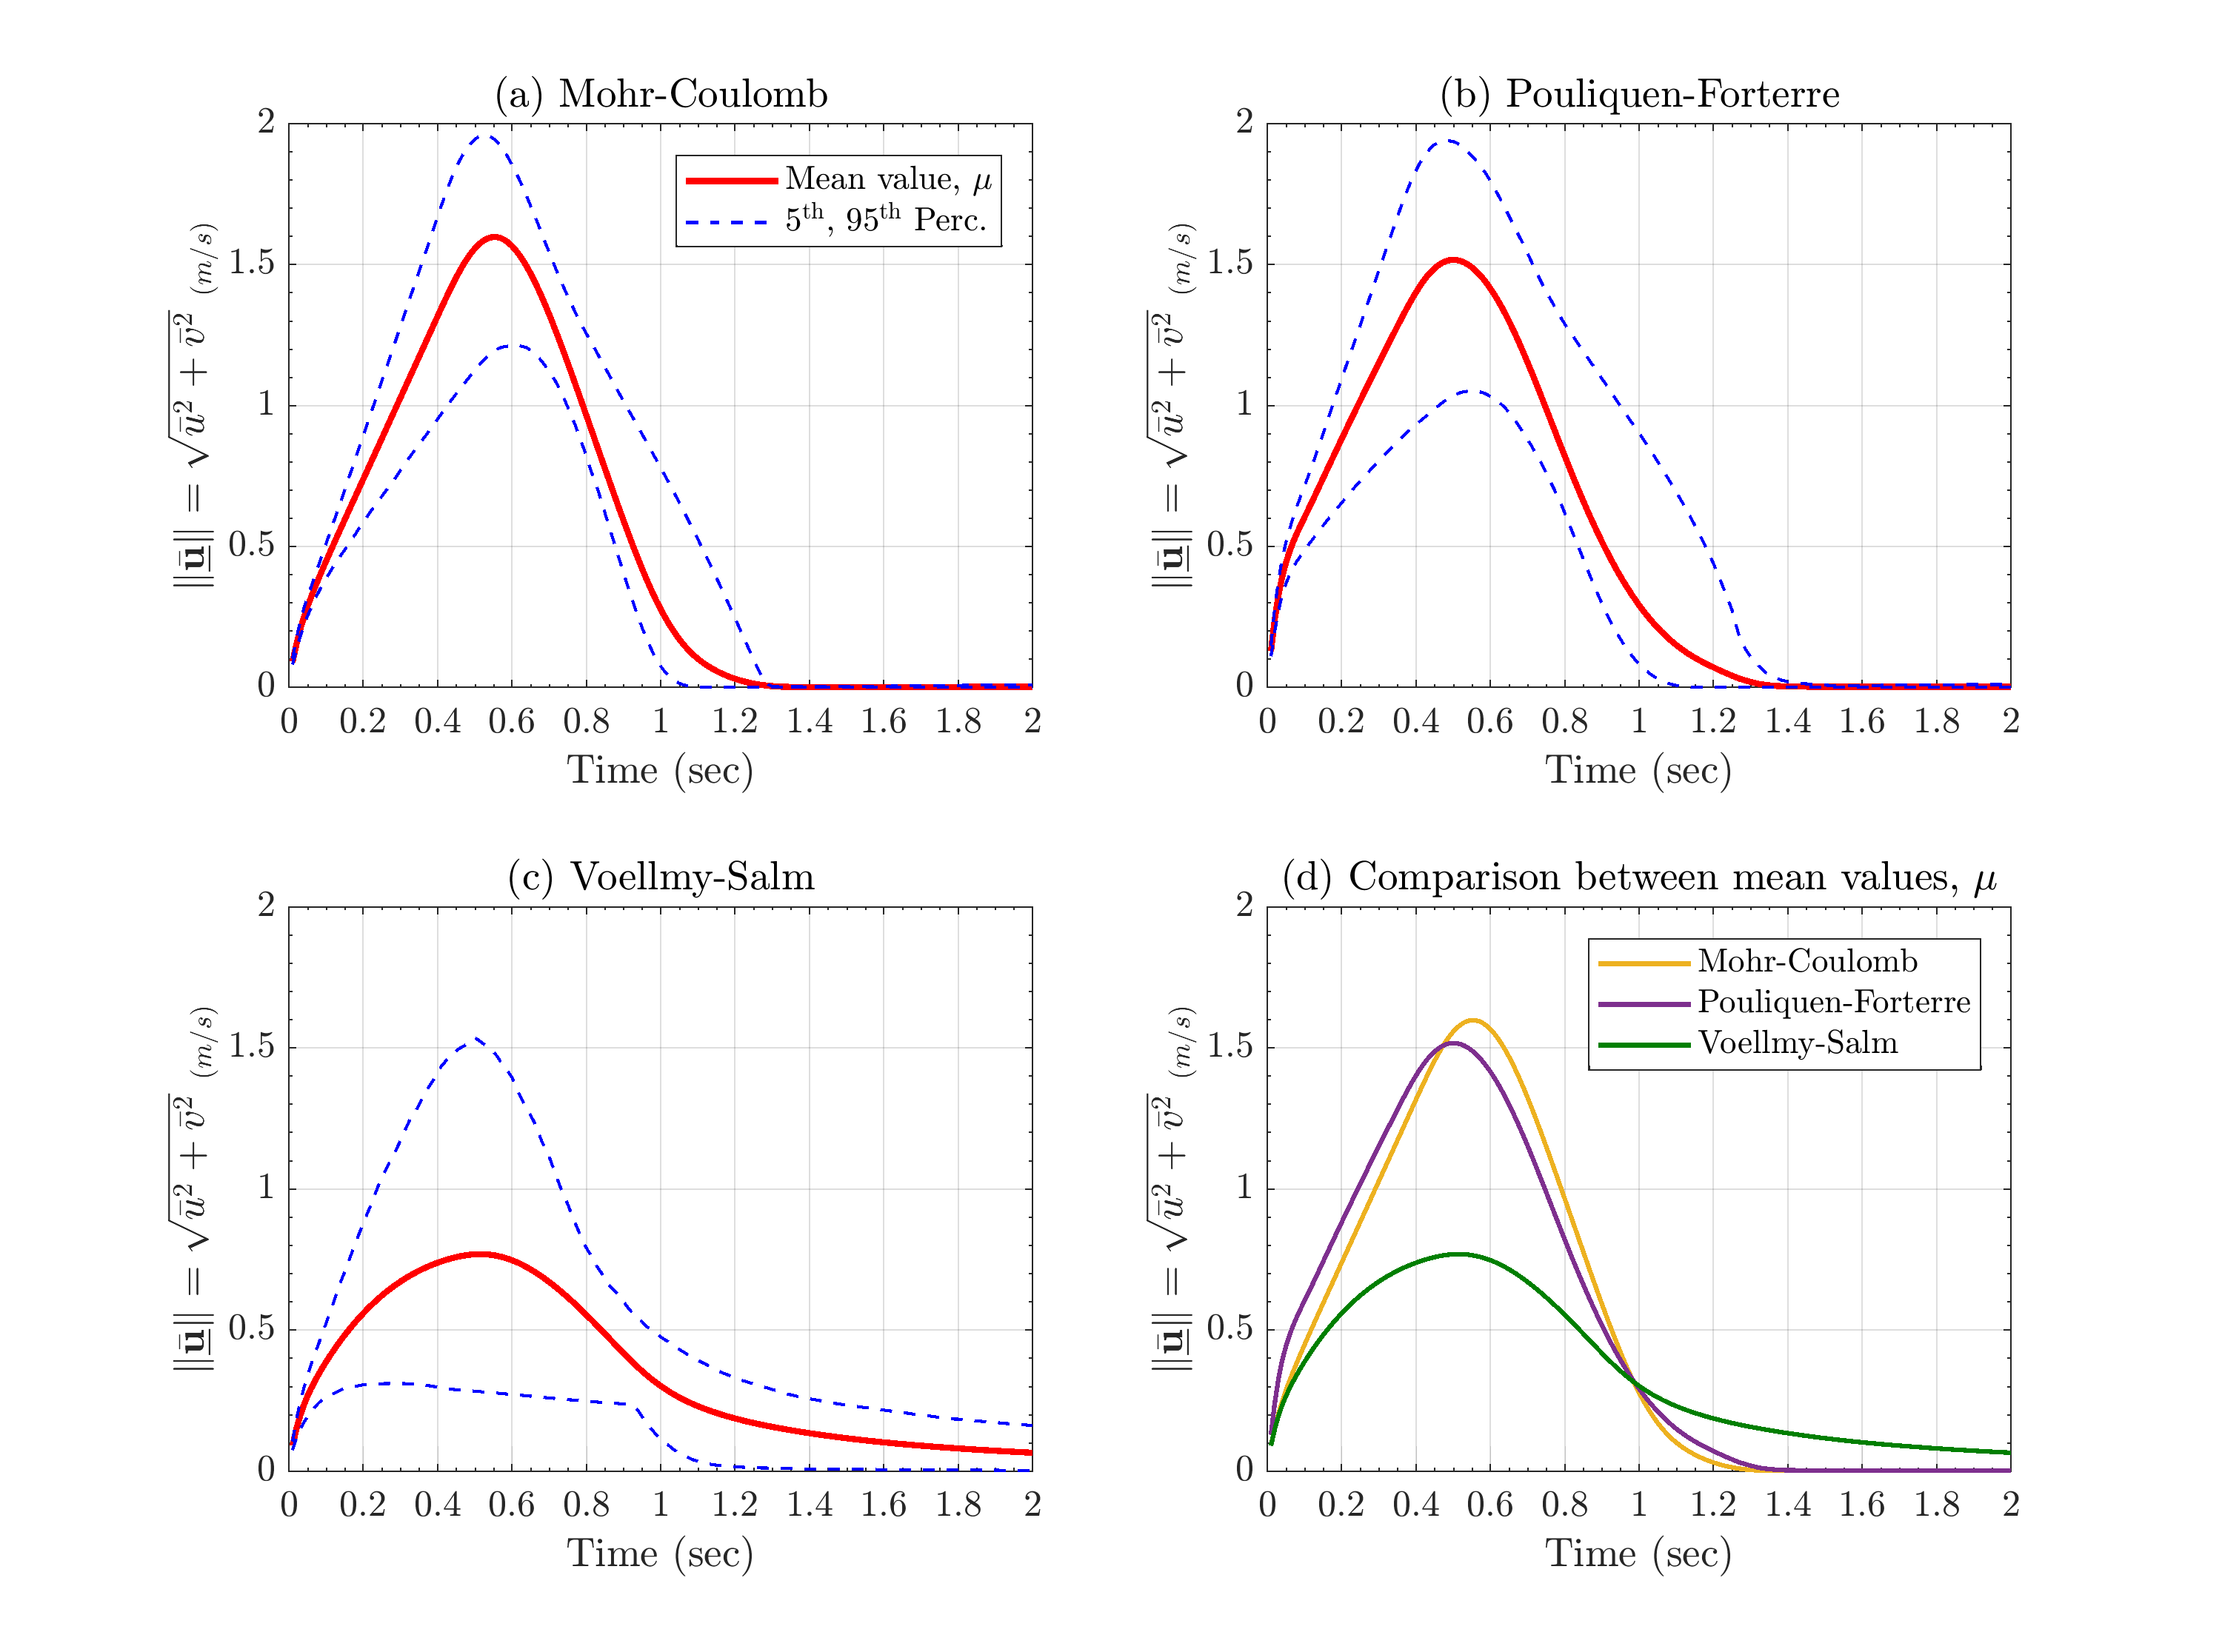
\includegraphics[width=1\textwidth]{InclinedPlane/Velocity/Vel_SpatialRec.png}
        \caption{Comparison between mean values of flow velocity, $\Vert \underline{\mathbf{u}} \Vert(L,t)$, recorded at locations of interest, $L_i, \ _{i=1,...,4}$.}
        \label{fig:Ramp-Vel-spatial}
\end{figure}

\subsubsection{Froude Number}
\begin{figure}[H]
	\begin{minipage}[b]{0.5\linewidth}
    	\centering
    	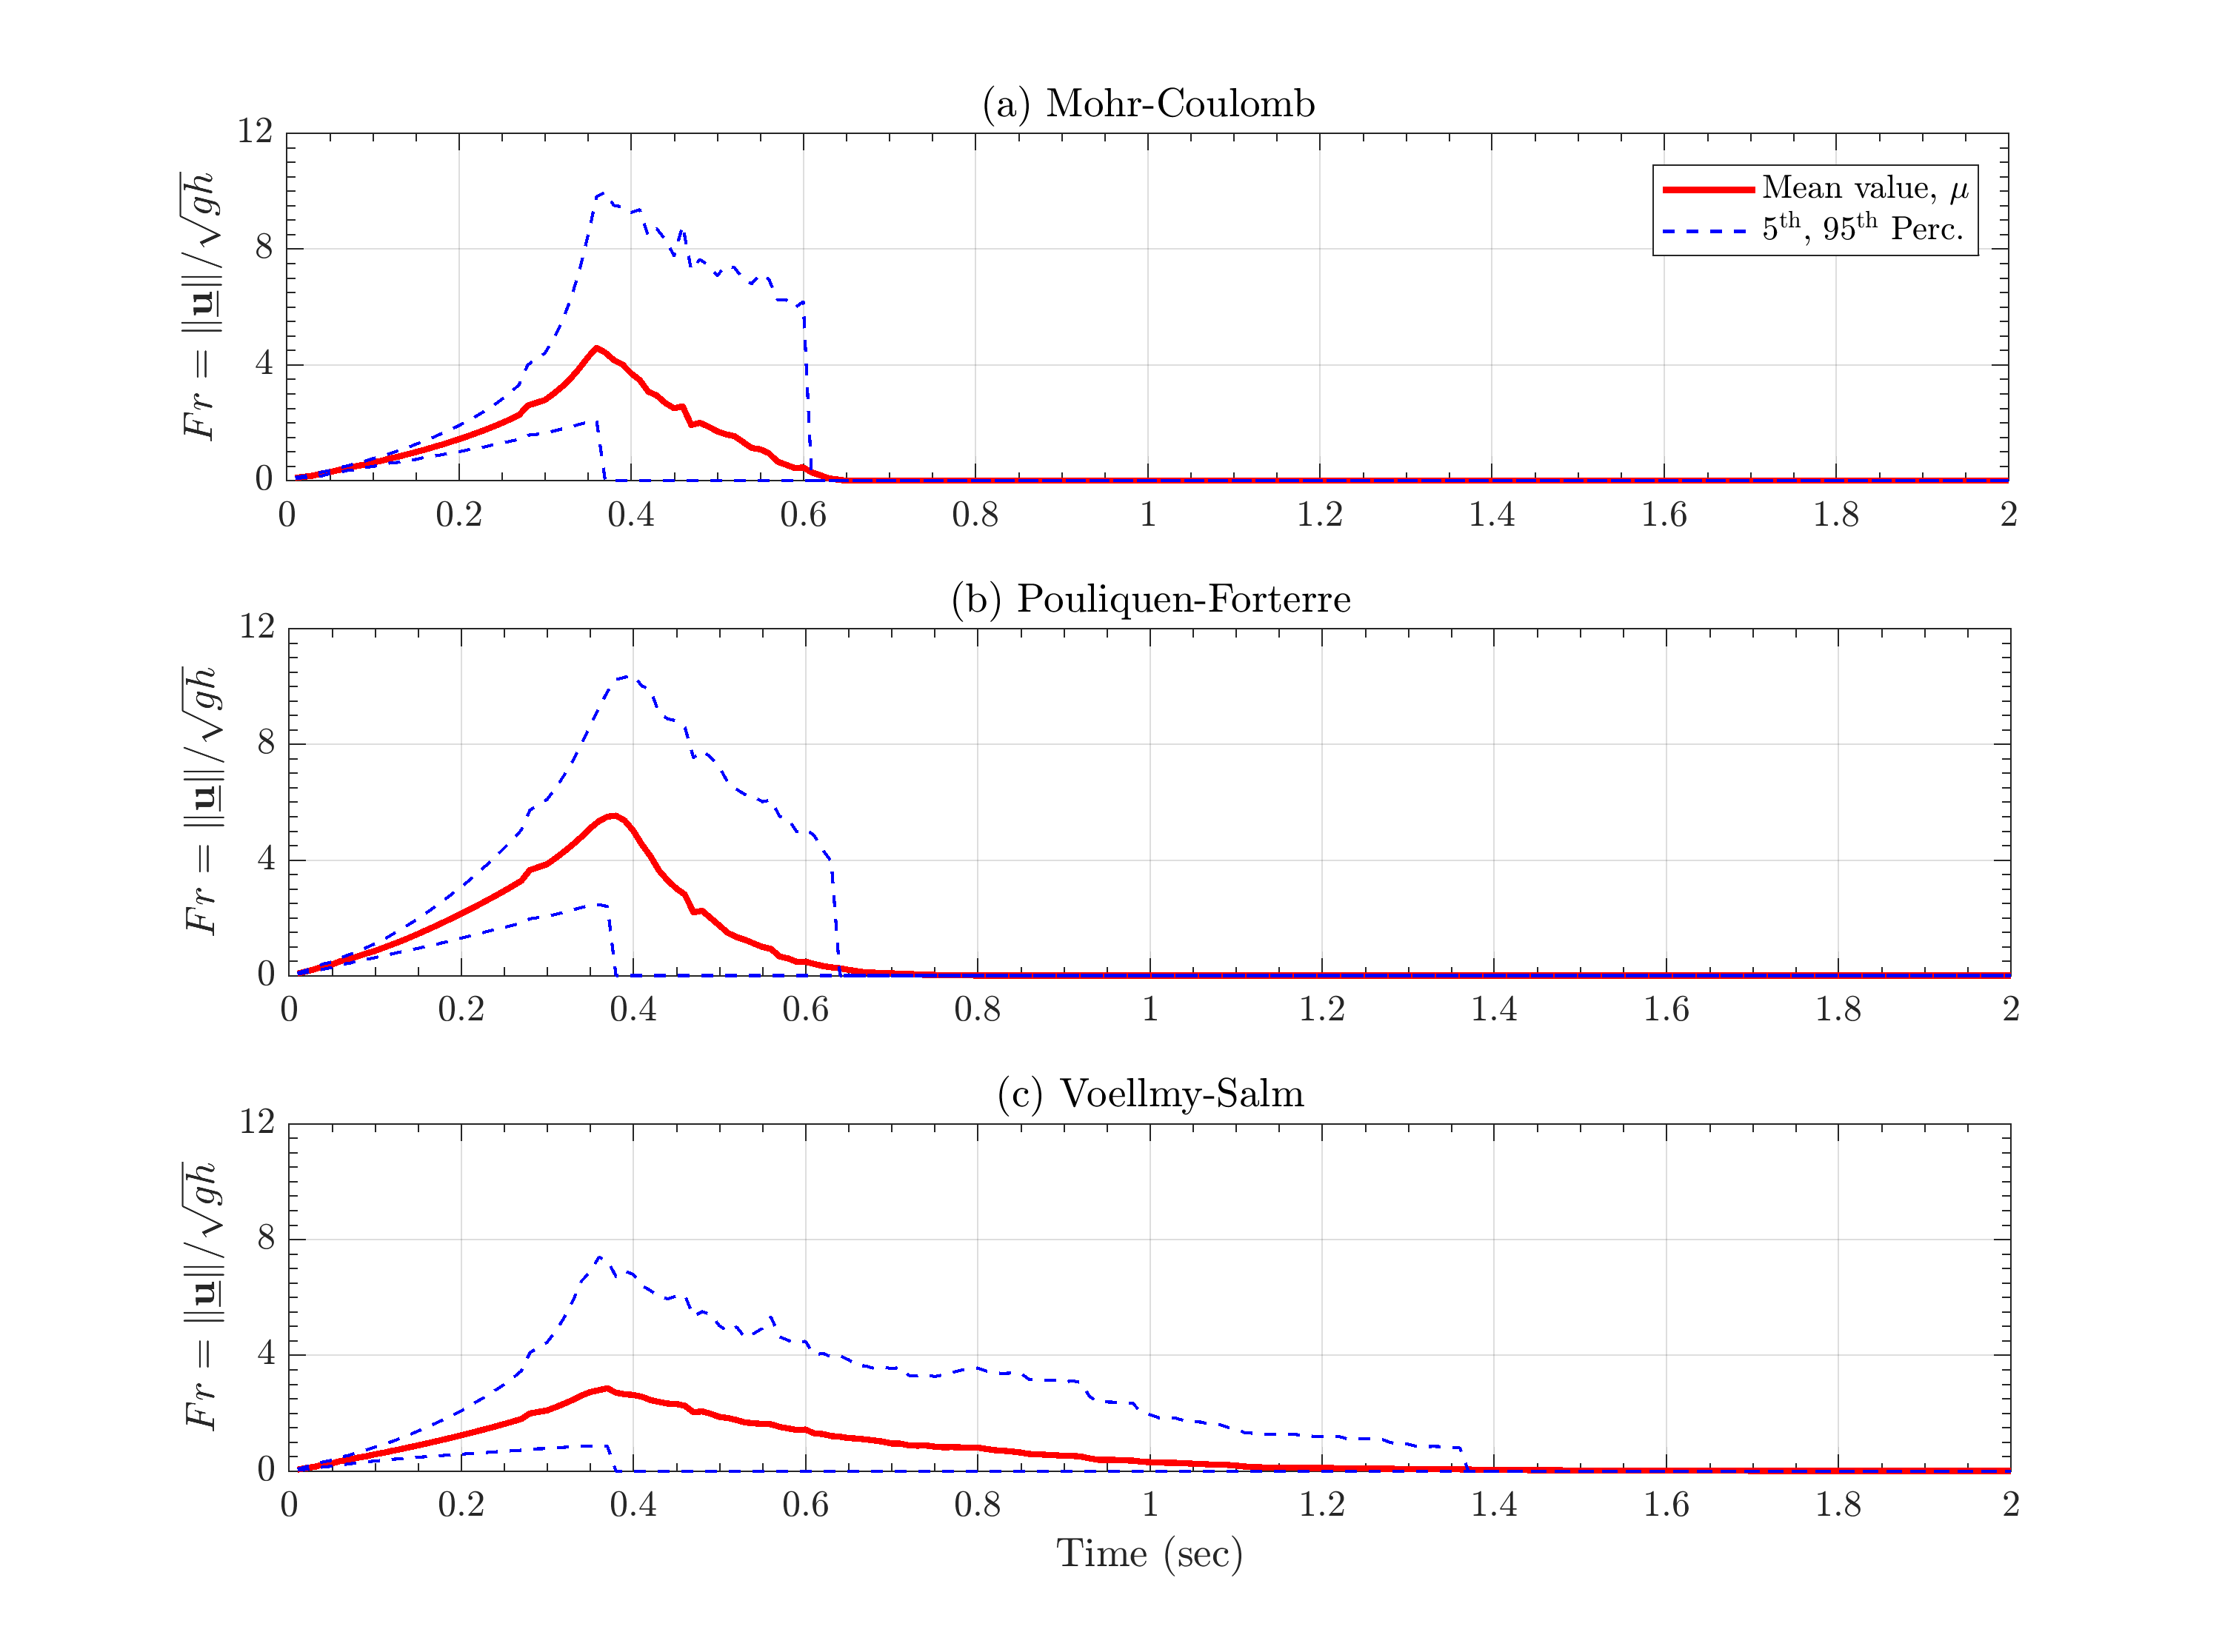
\includegraphics[width=1\textwidth]{InclinedPlane/Froude/Fr_L1.png}
    	\subcaption{$L=(-0.7,0)$, slumping pile location.}
    	\label{fig:Ramp-L1-Fr}
	\end{minipage}
	\begin{minipage}[b]{0.5\linewidth}
		\centering
		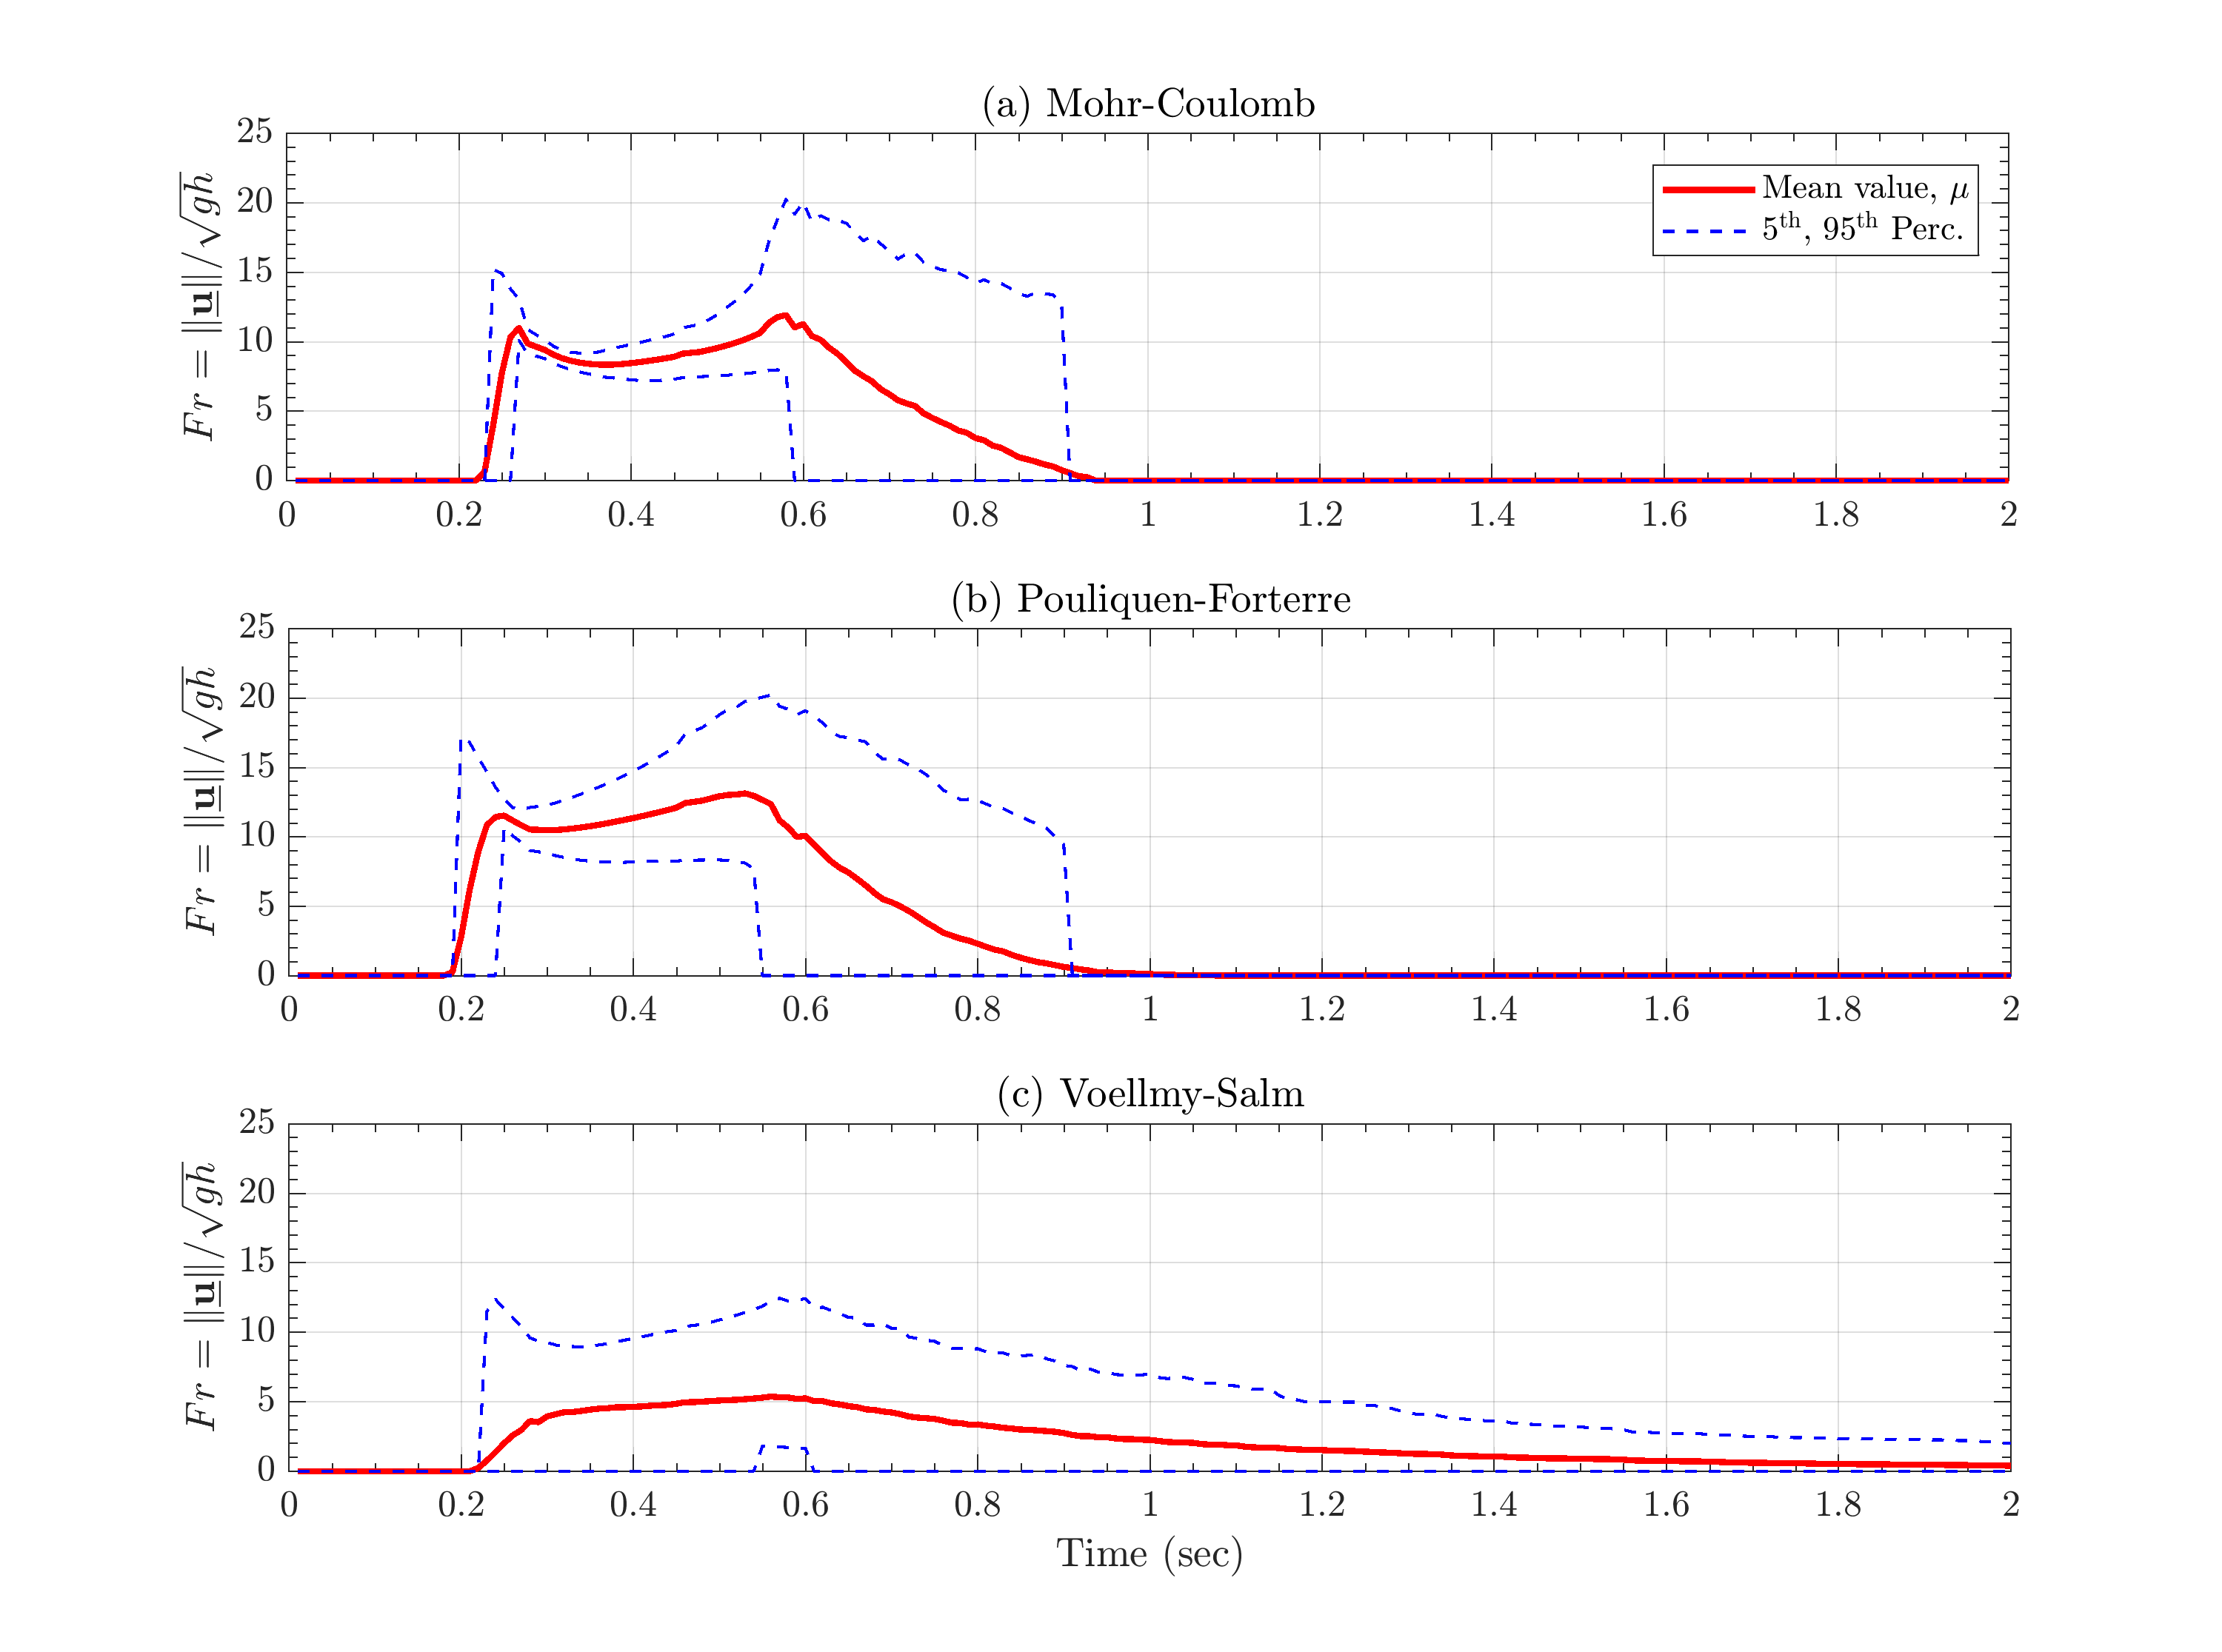
\includegraphics[width=1\textwidth]{InclinedPlane/Froude/Fr_L2.png}
    	\subcaption{$L=(-0.35,0)$, middle point on inclined plane.}
    	\label{fig:Ramp-L2-Fr}
    \end{minipage}

	\begin{minipage}[b]{0.5\linewidth}
    	\centering
    	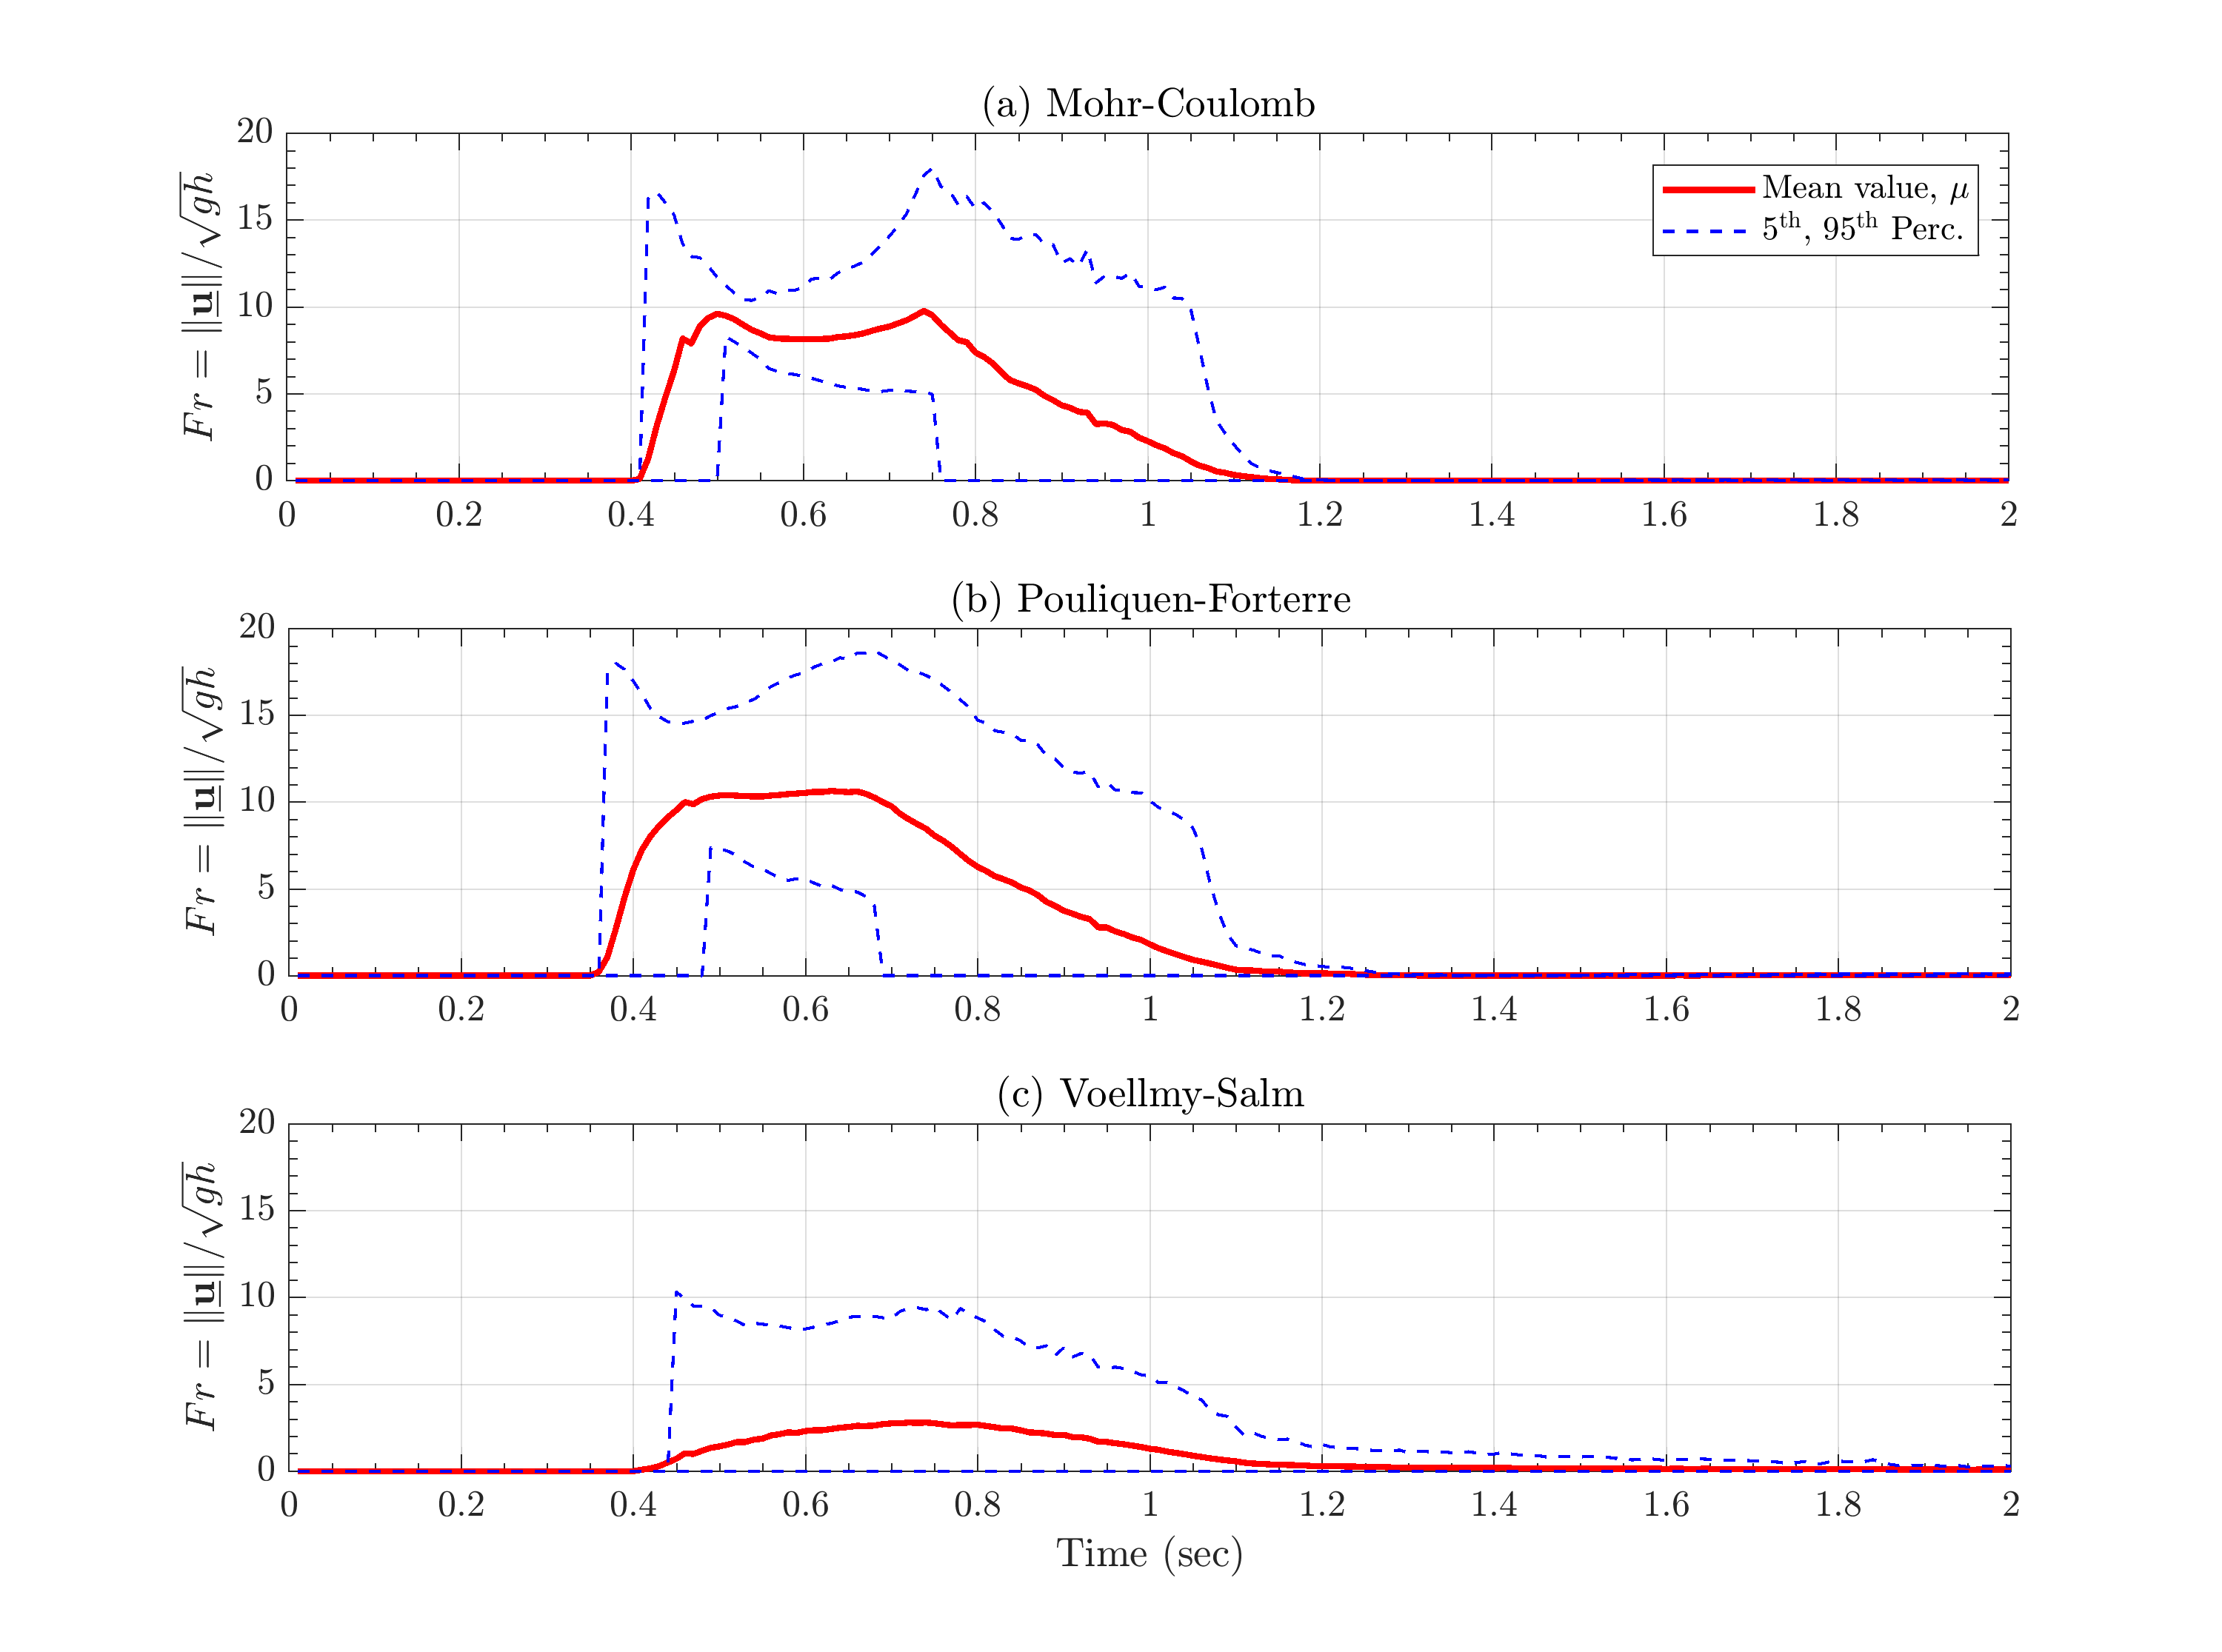
\includegraphics[width=1\textwidth]{InclinedPlane/Froude/Fr_L3.png}
    	\subcaption{$L=(0,0)$, inclined and runout planes' joint location.}
    	\label{fig:Ramp-L3-Fr}
	\end{minipage}
	\begin{minipage}[b]{0.5\linewidth}
		\centering
		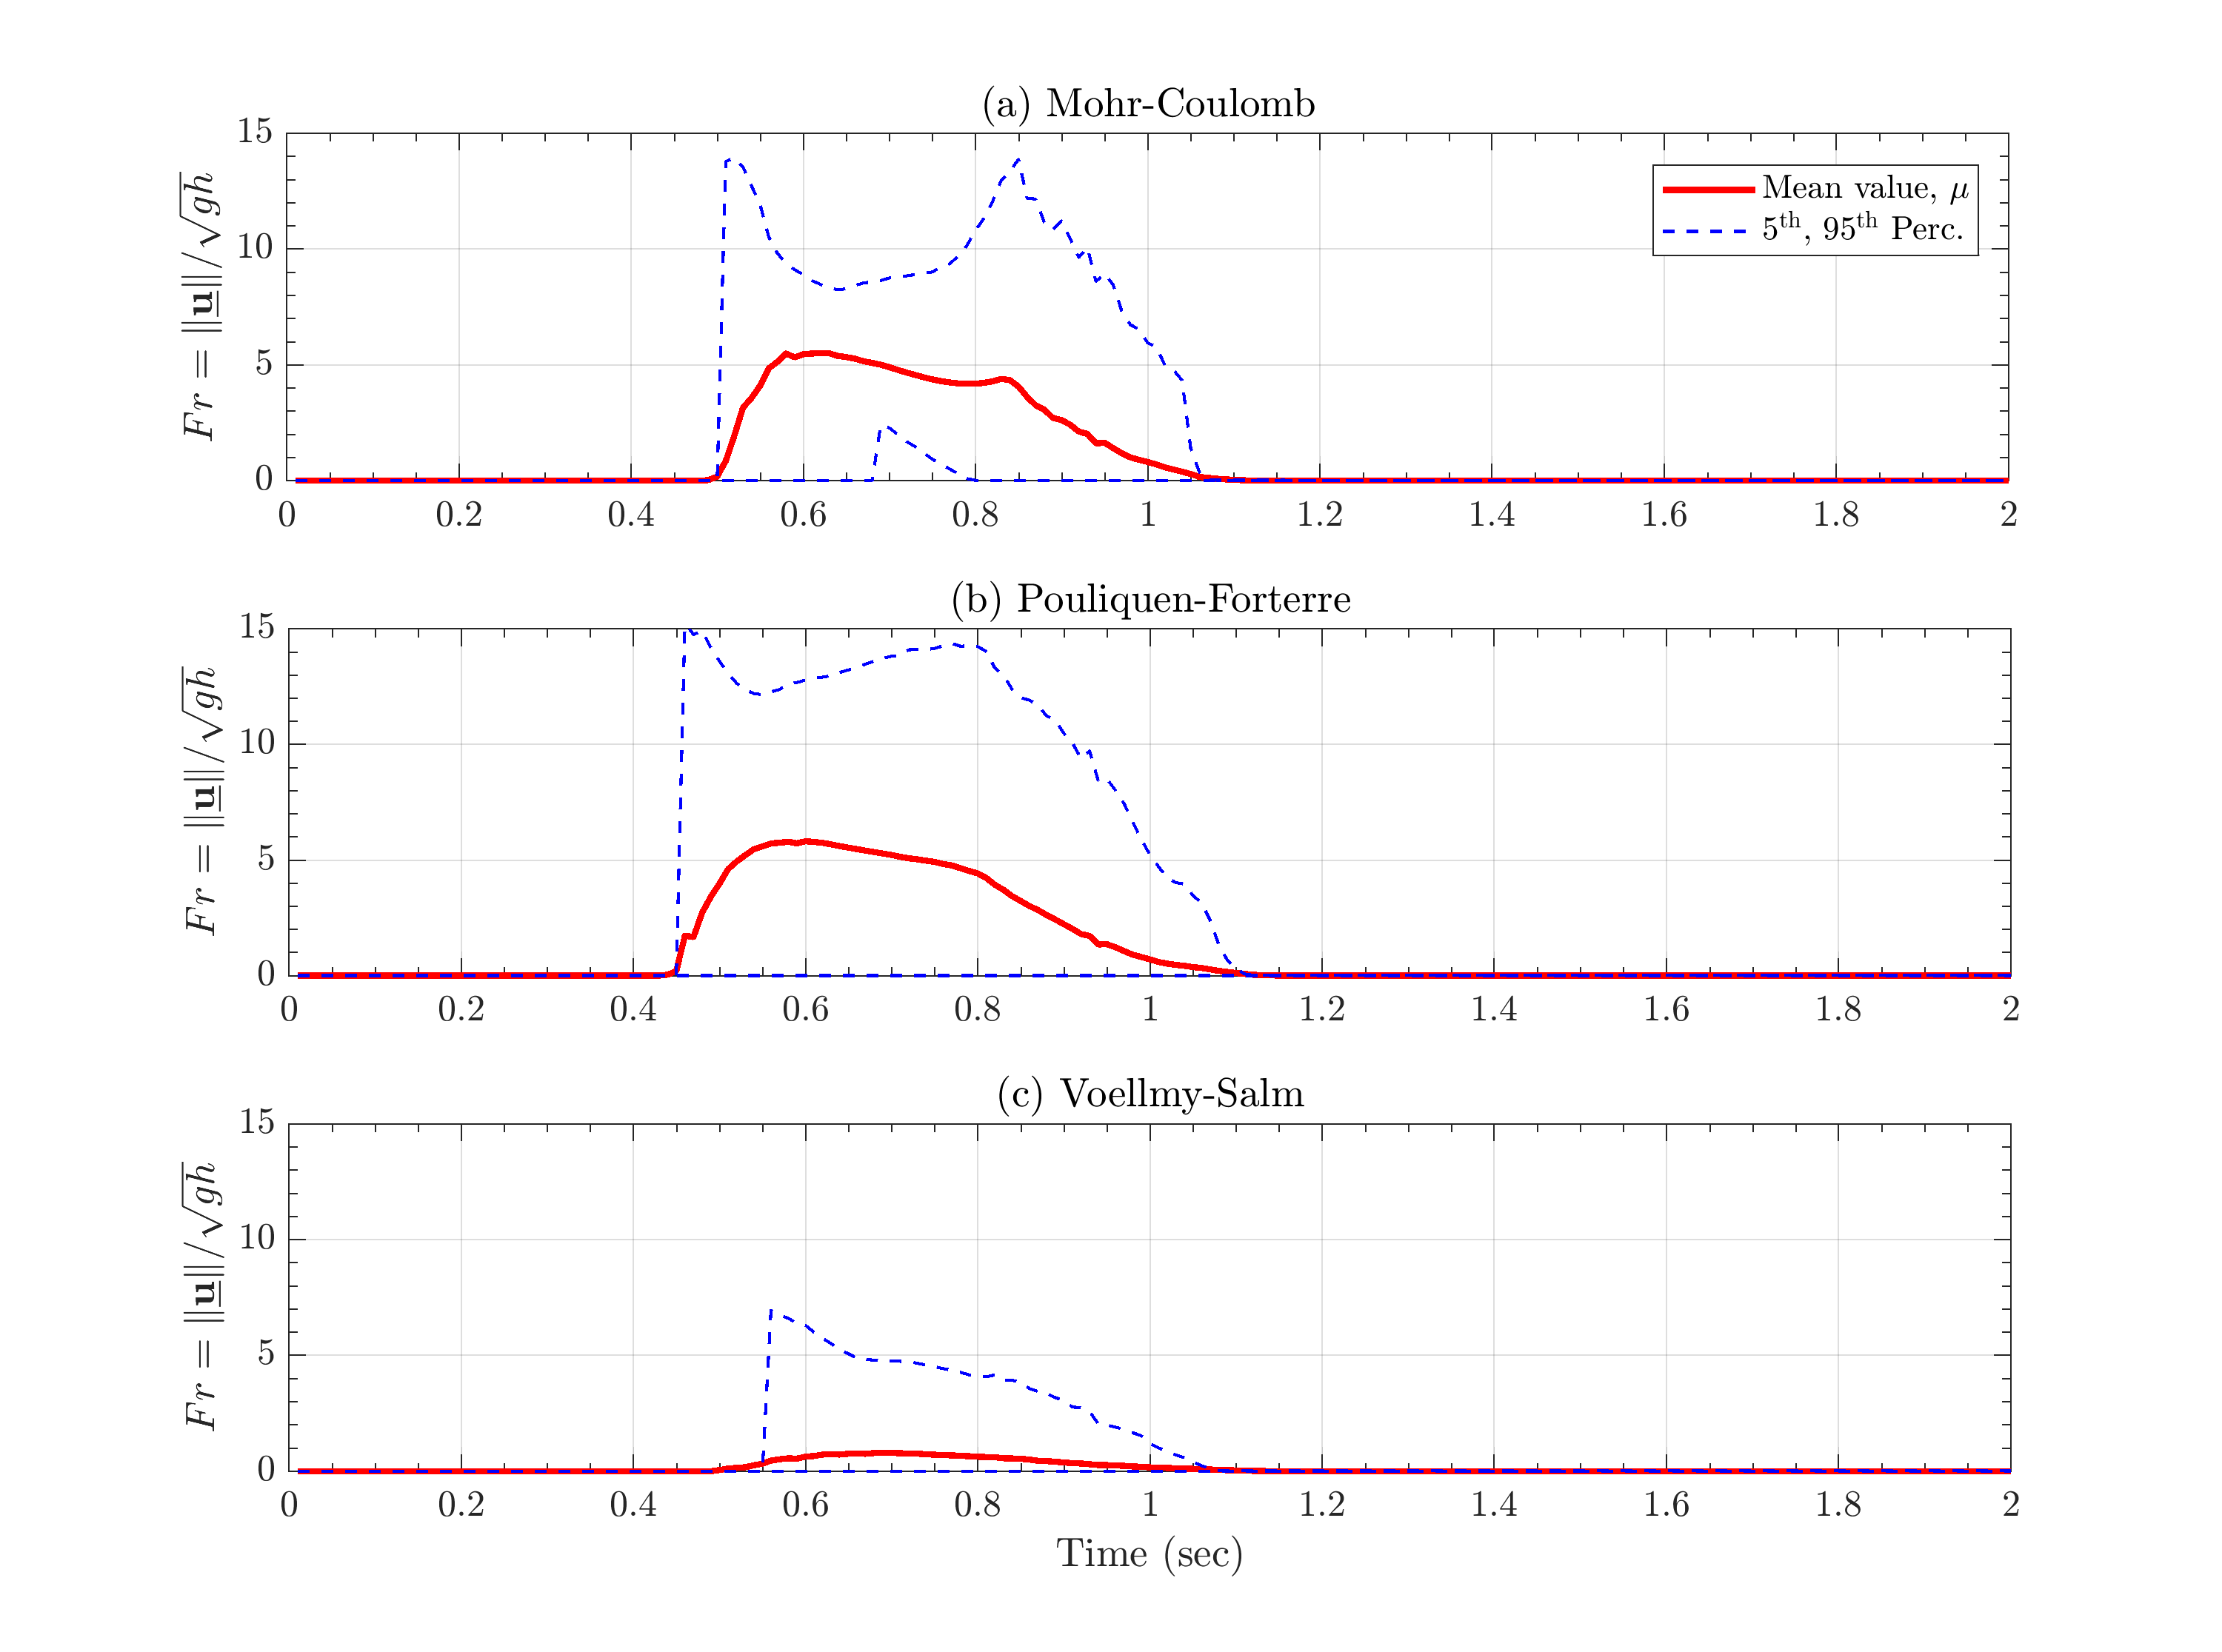
\includegraphics[width=1\textwidth]{InclinedPlane/Froude/Fr_L4.png}
    	\subcaption{$L=(0.15,0)$, a location on runout plane.}
    	\label{fig:Ramp-L4-Fr}
    \end{minipage}
    \caption{Records of flow velocity, $\Vert \underline{\mathbf{u}} \Vert(L,t)$.}
    \label{fig:Ramp-LM-Fr}
\end{figure}

\begin{figure}[H]
        \centering
        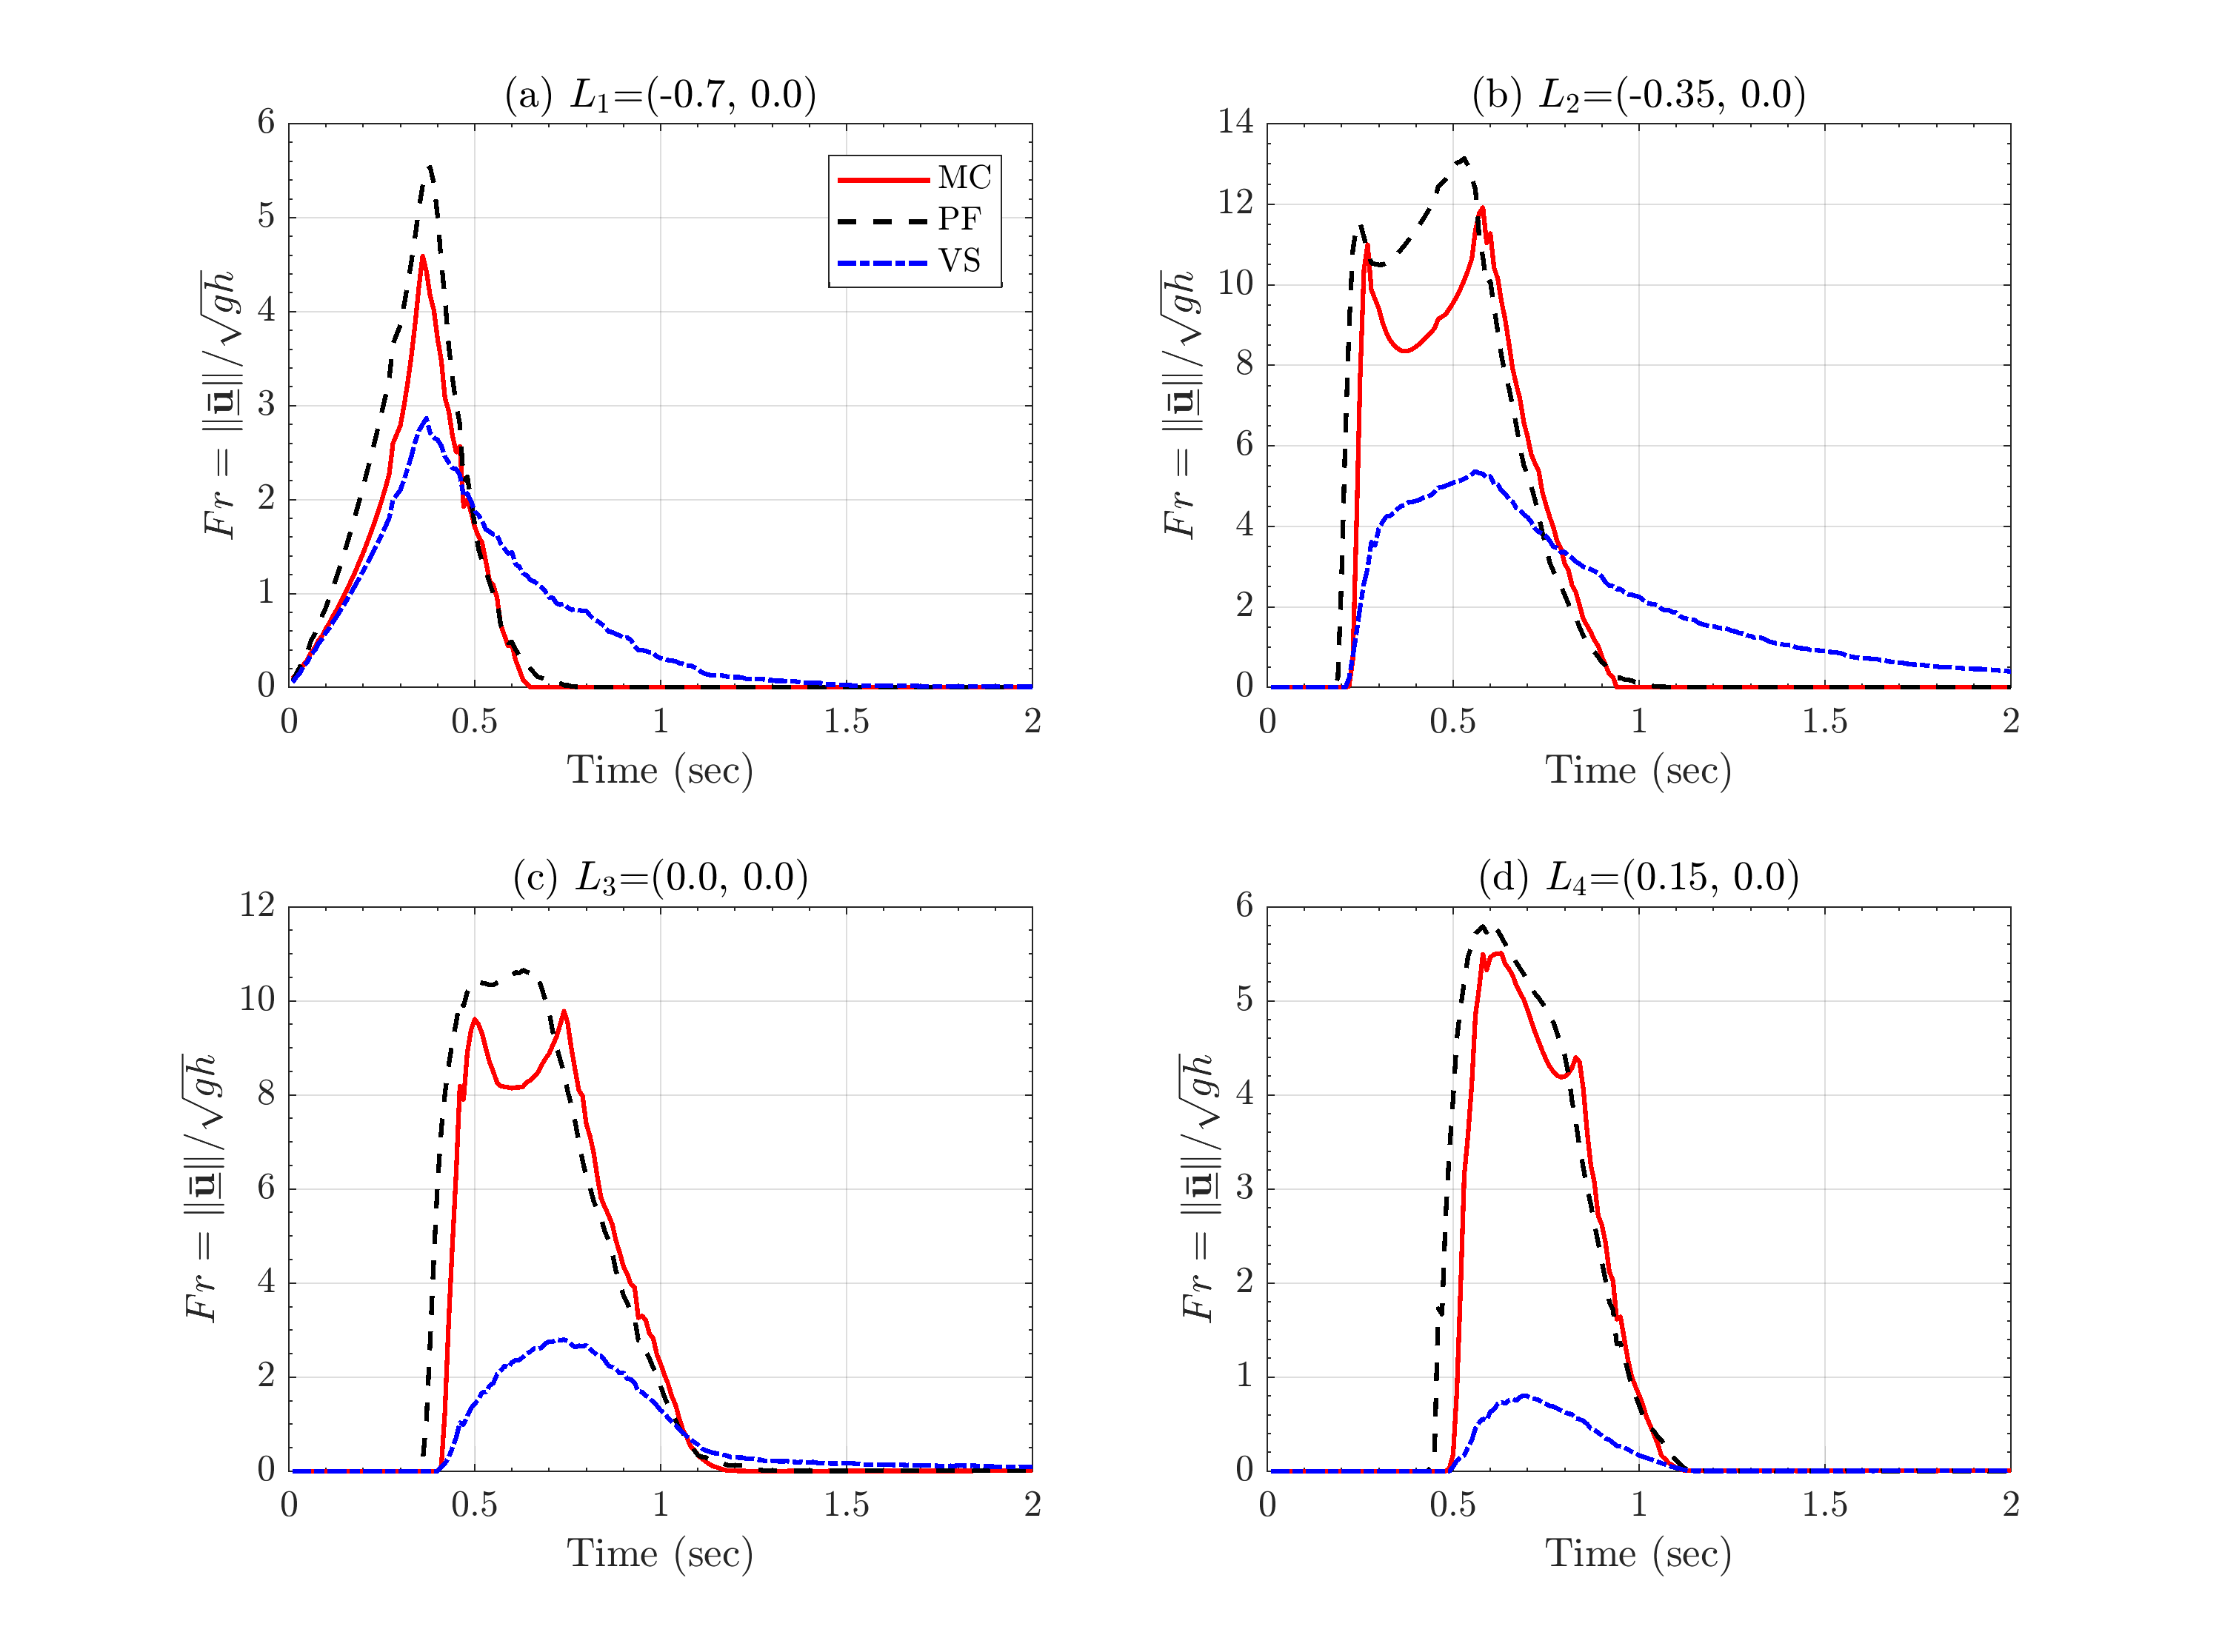
\includegraphics[width=1\textwidth]{InclinedPlane/Froude/Fr_mean.png}
        \caption{Comparison between mean values of flow velocity, $\Vert \underline{\mathbf{u}} \Vert(L,t)$, recorded at locations of interest, $L_i, \ _{i=1,...,4}$.}
        \label{fig:Ramp-LM-Fr-means}
\end{figure}

\begin{figure}[H]
        \centering
        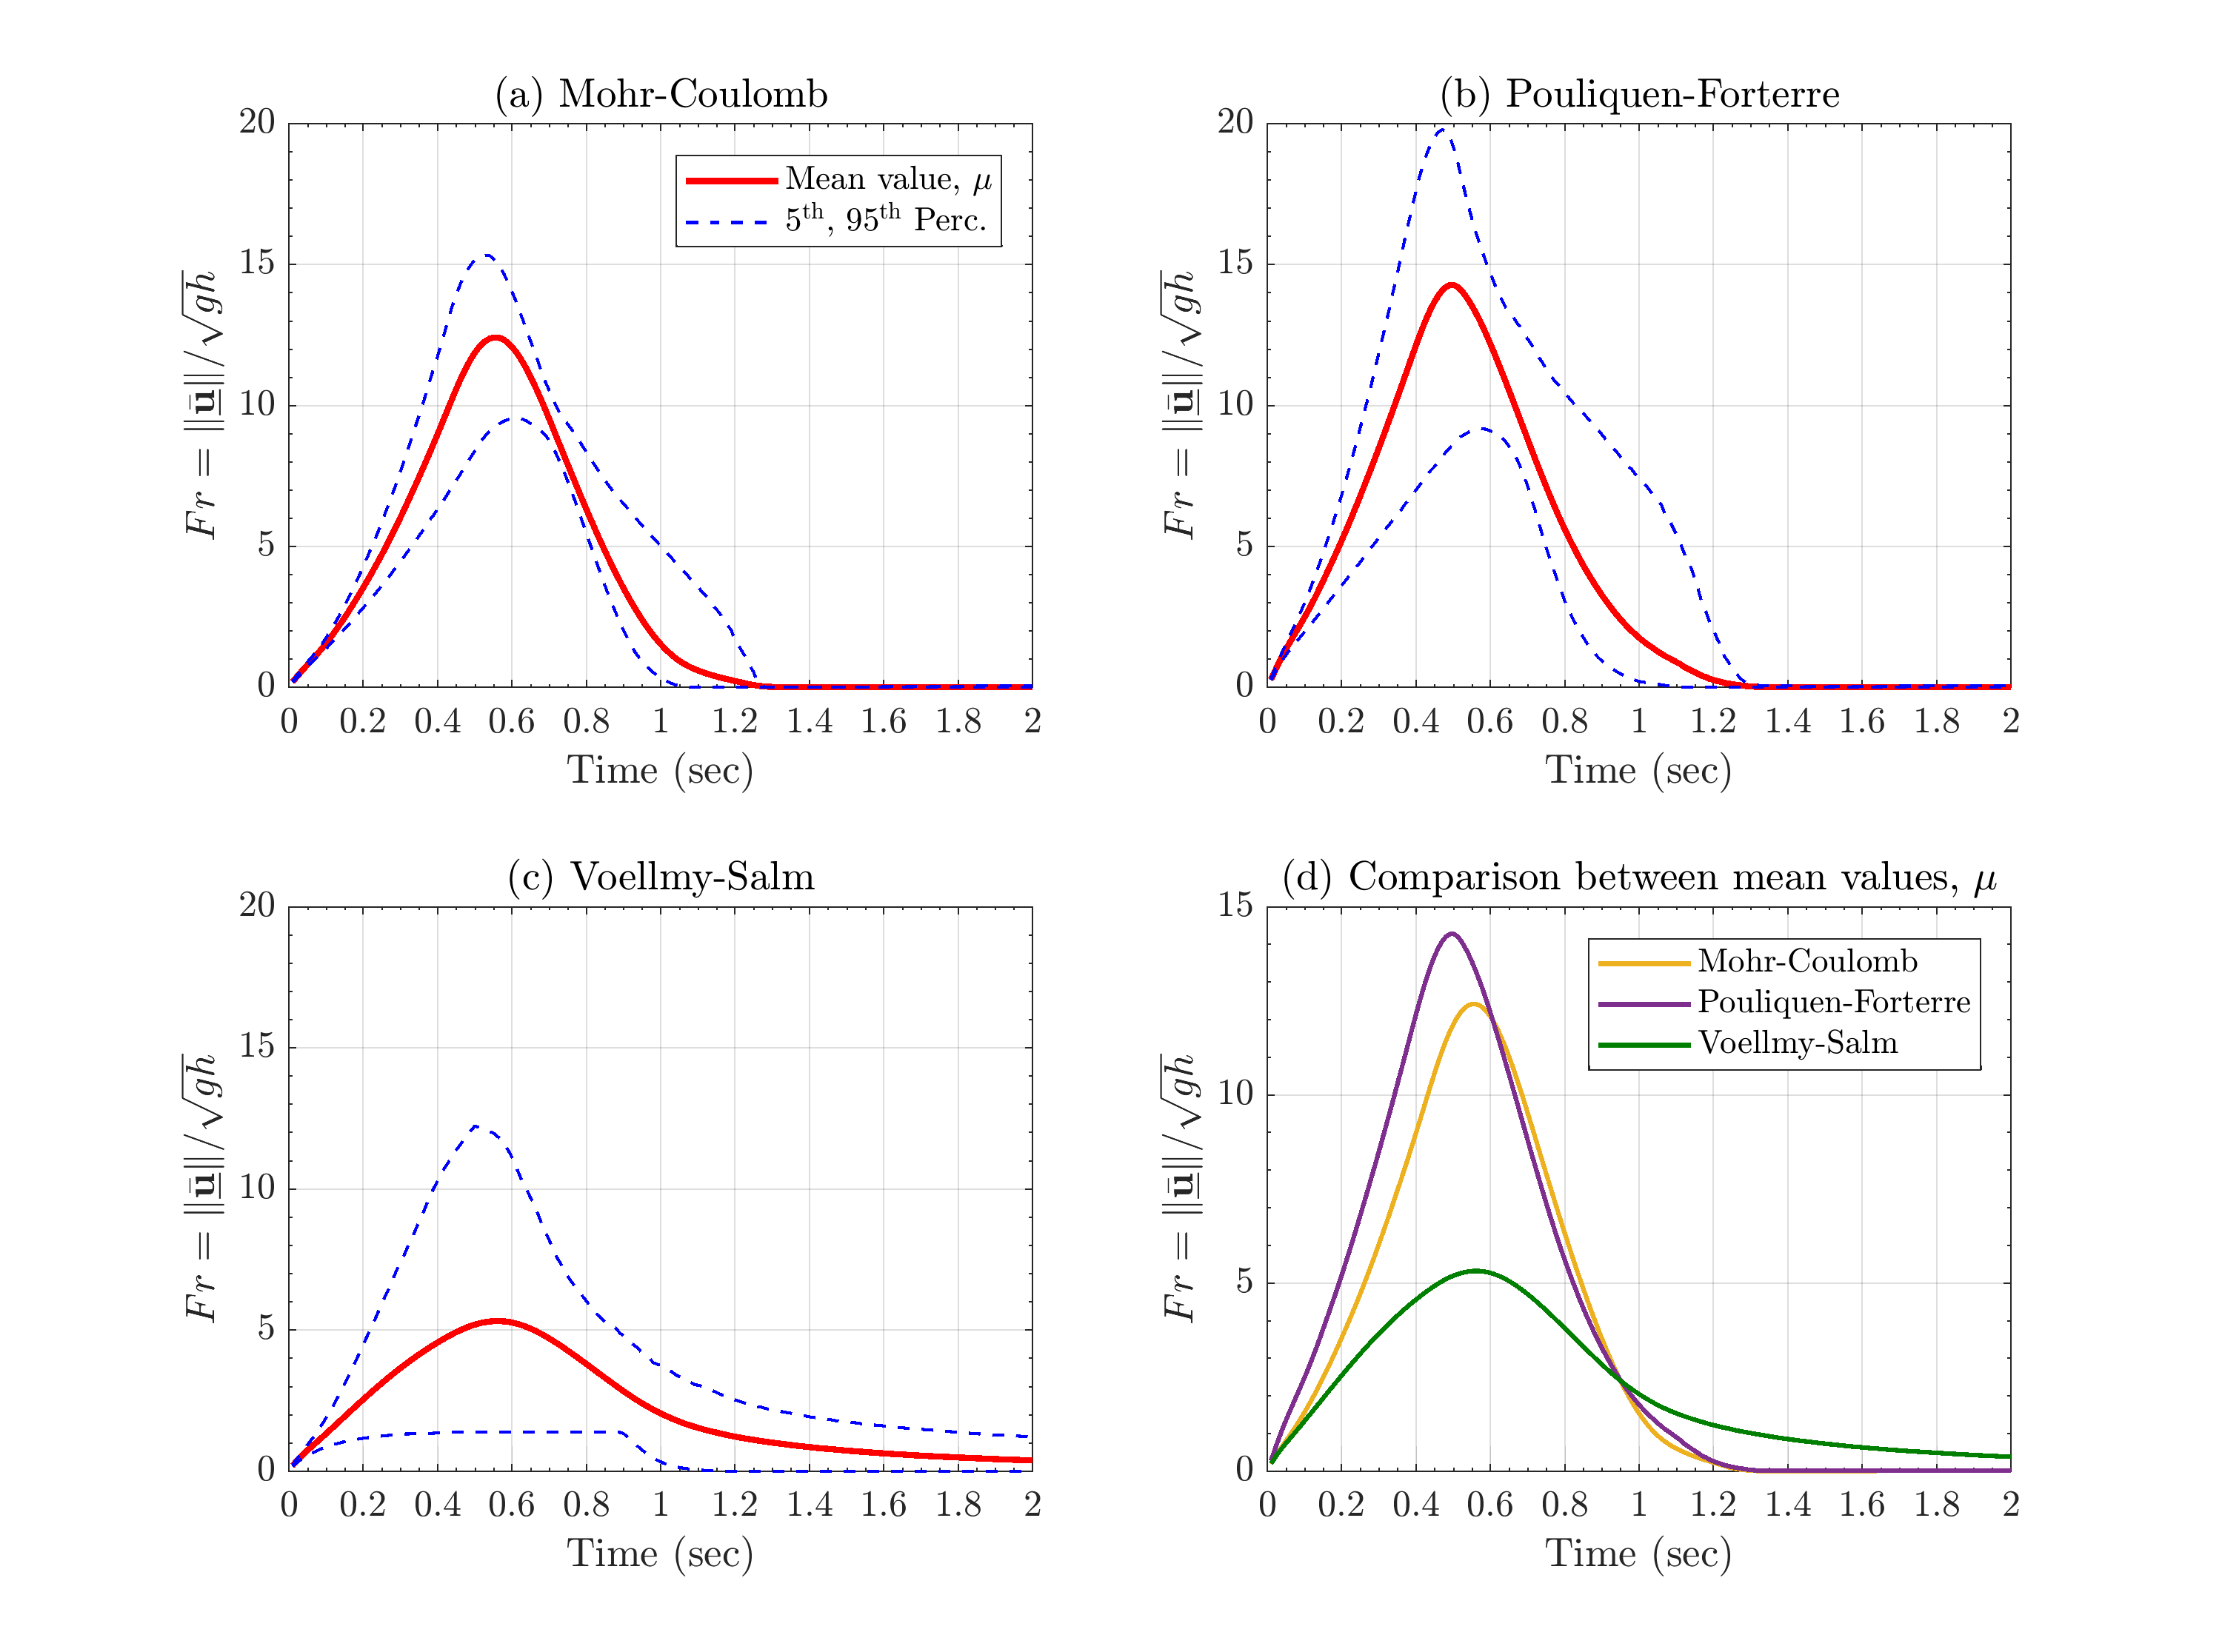
\includegraphics[width=1\textwidth]{InclinedPlane/Froude/Fr_SpatialRec.png}
        \caption{Comparison between mean values of flow velocity, $\Vert \underline{\mathbf{u}} \Vert(L,t)$, recorded at locations of interest, $L_i, \ _{i=1,...,4}$.}
        \label{fig:Ramp-Fr-spatial}
\end{figure}

\subsubsection{Flow Acceleration}
\begin{figure}[H]
	\begin{minipage}[b]{0.5\linewidth}
    	\centering
    	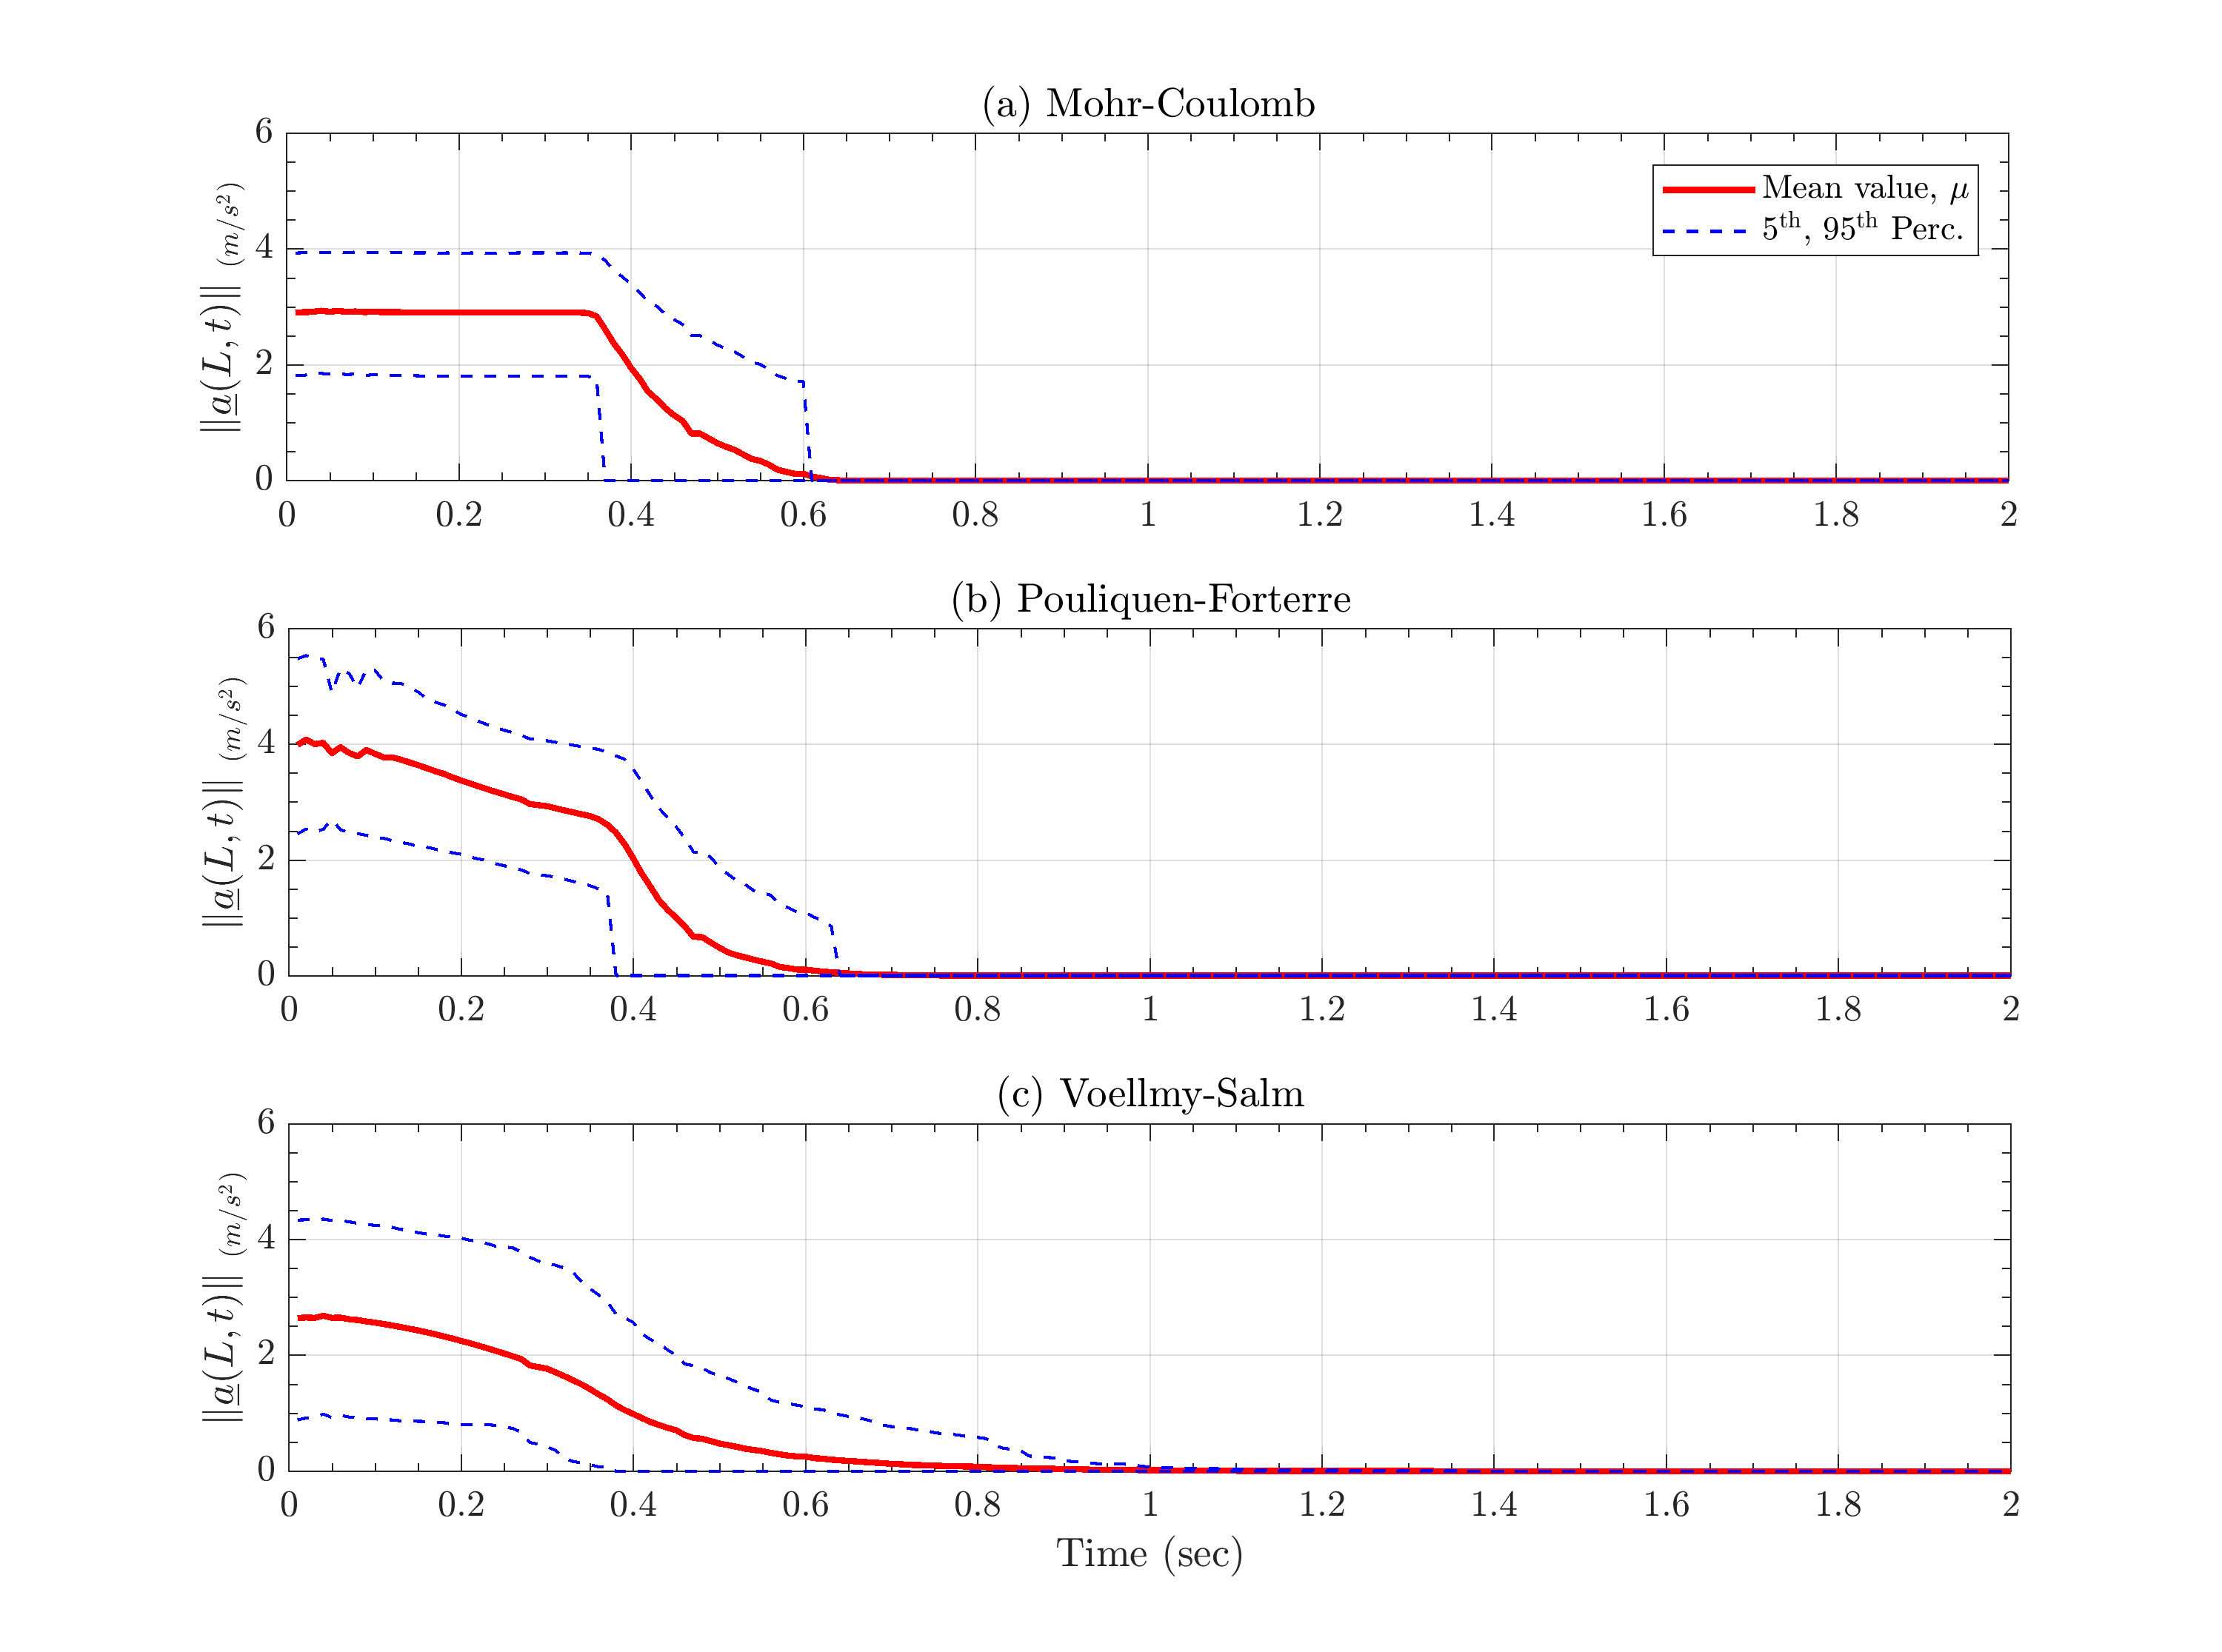
\includegraphics[width=1\textwidth]{InclinedPlane/Acceleration/accel_L1R.png}
    	\subcaption{$L=(-0.7,0)$, slumping pile location.}
    	\label{fig:Ramp-L1-AccR}
	\end{minipage}
	\begin{minipage}[b]{0.5\linewidth}
		\centering
		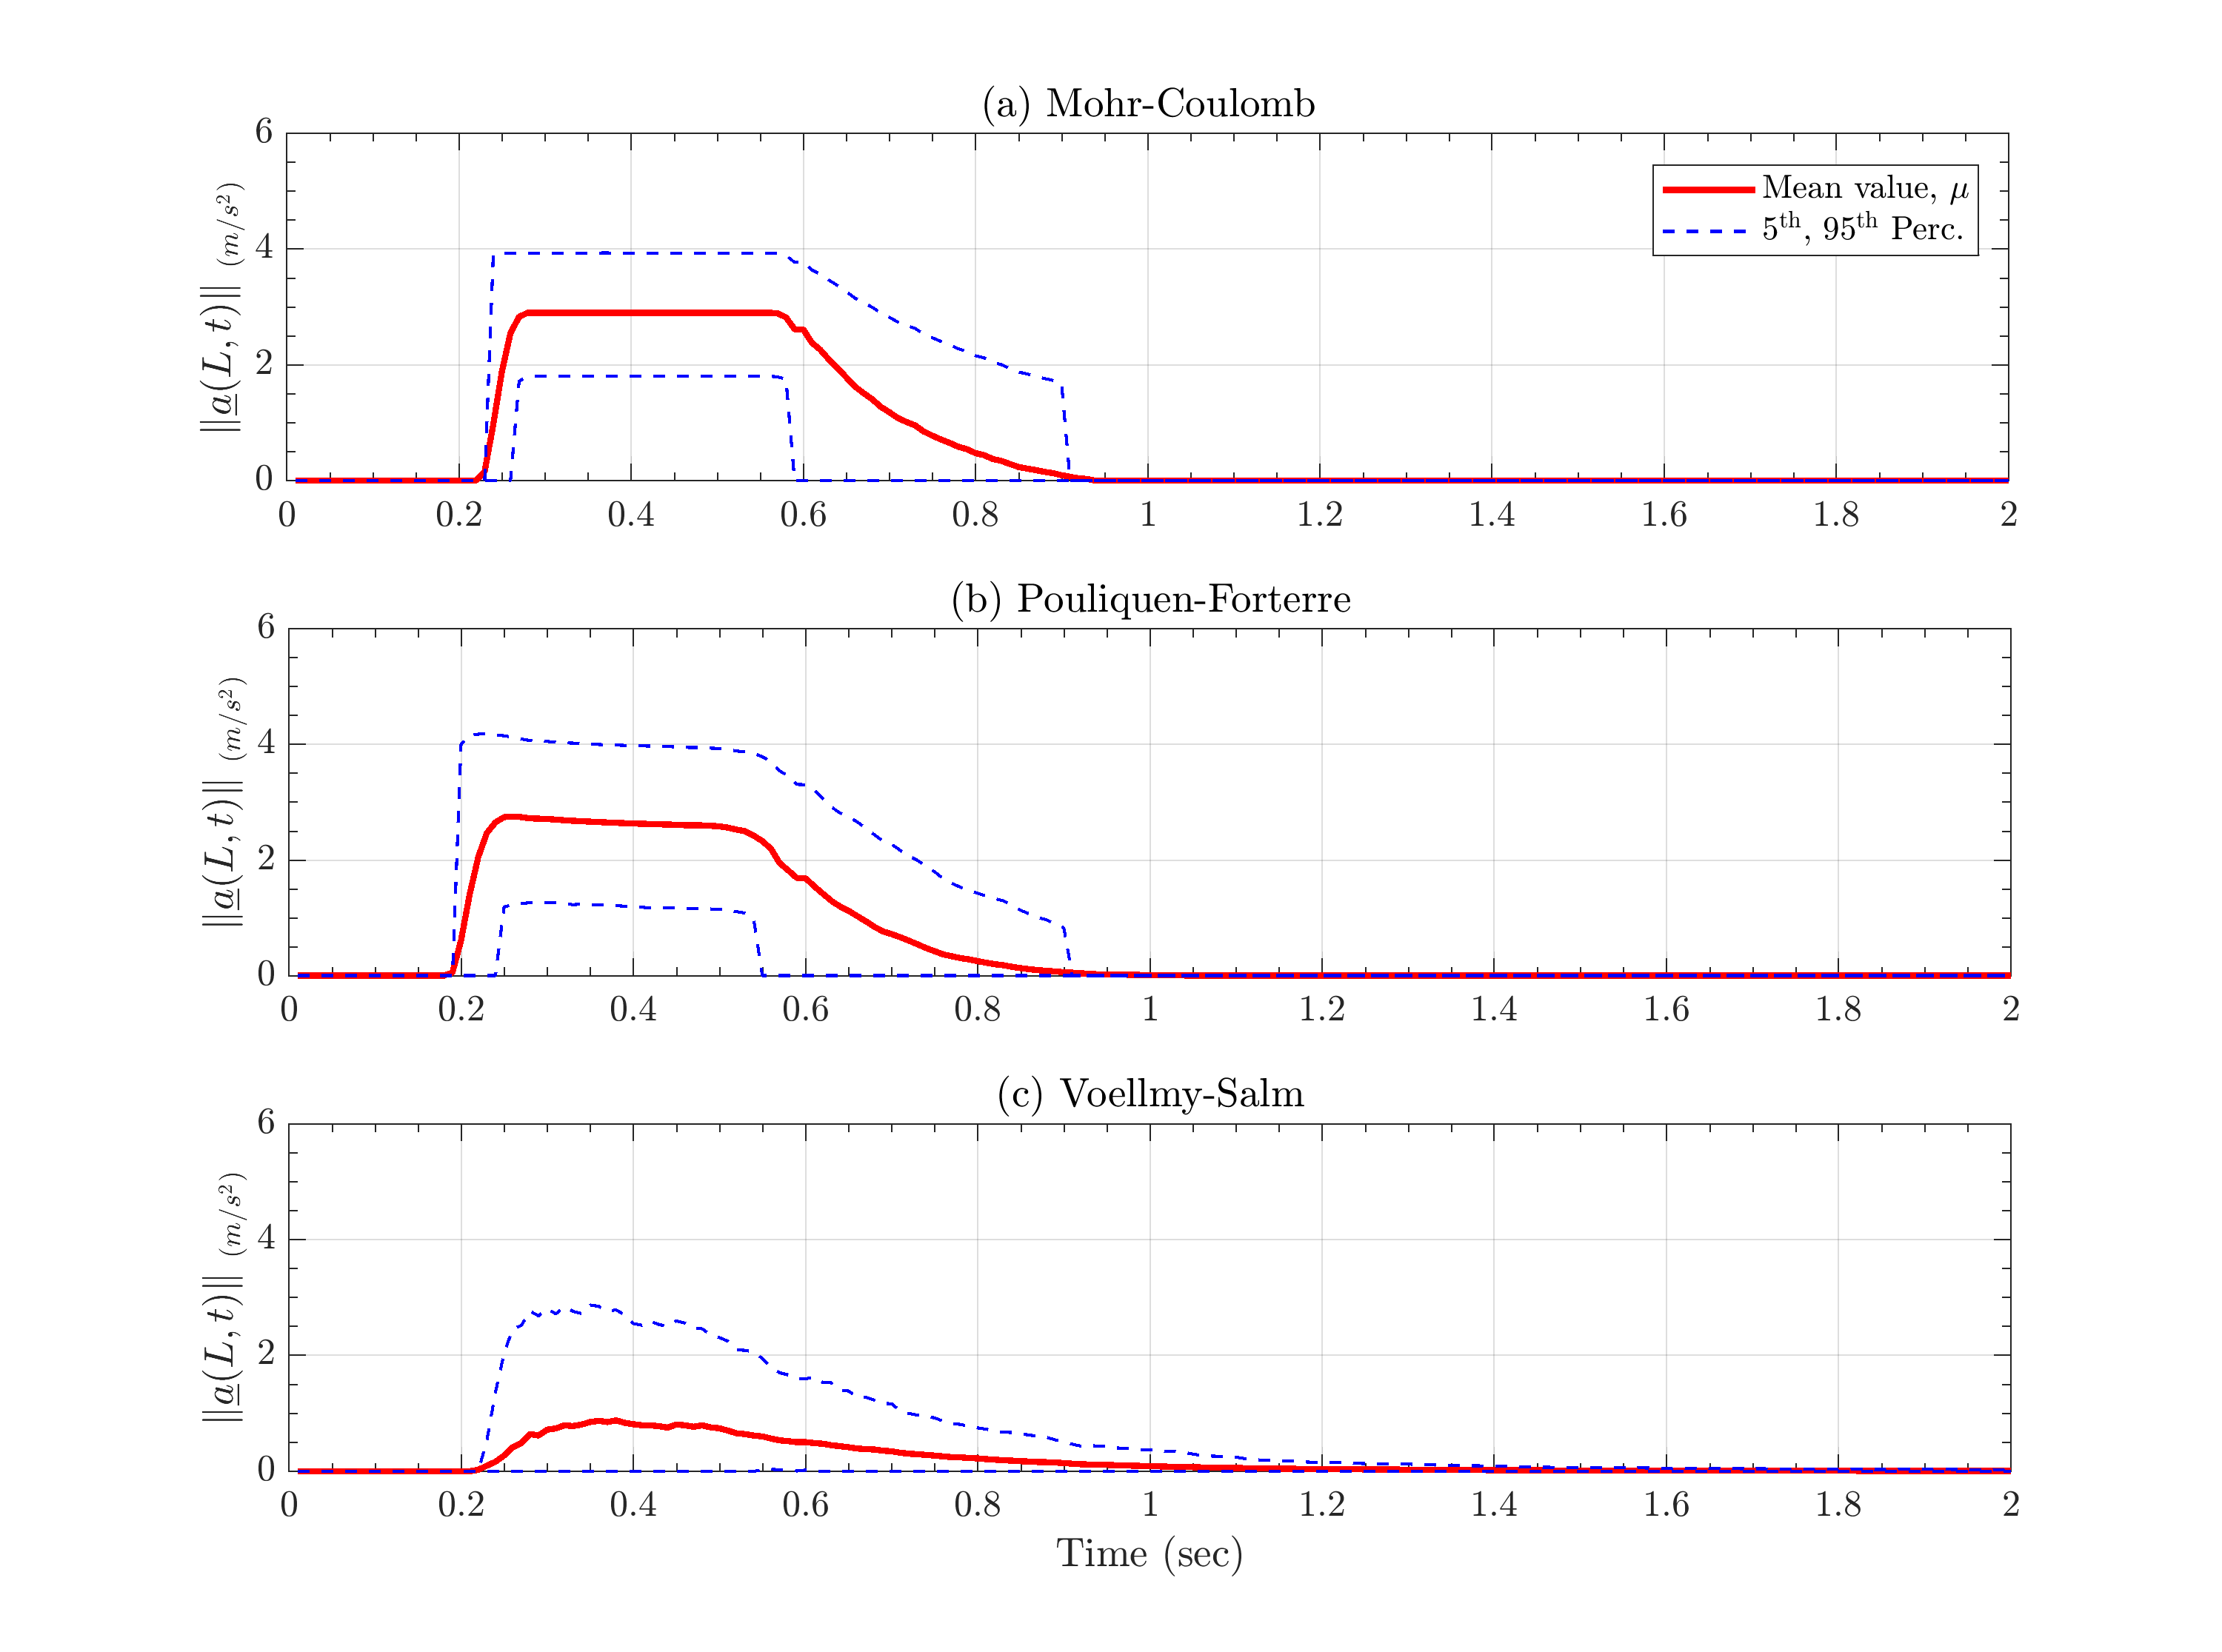
\includegraphics[width=1\textwidth]{InclinedPlane/Acceleration/accel_L2R.png}
    	\subcaption{$L=(-0.35,0)$, middle point on inclined plane.}
    	\label{fig:Ramp-L2-AccR}
    \end{minipage}

	\begin{minipage}[b]{0.5\linewidth}
    	\centering
    	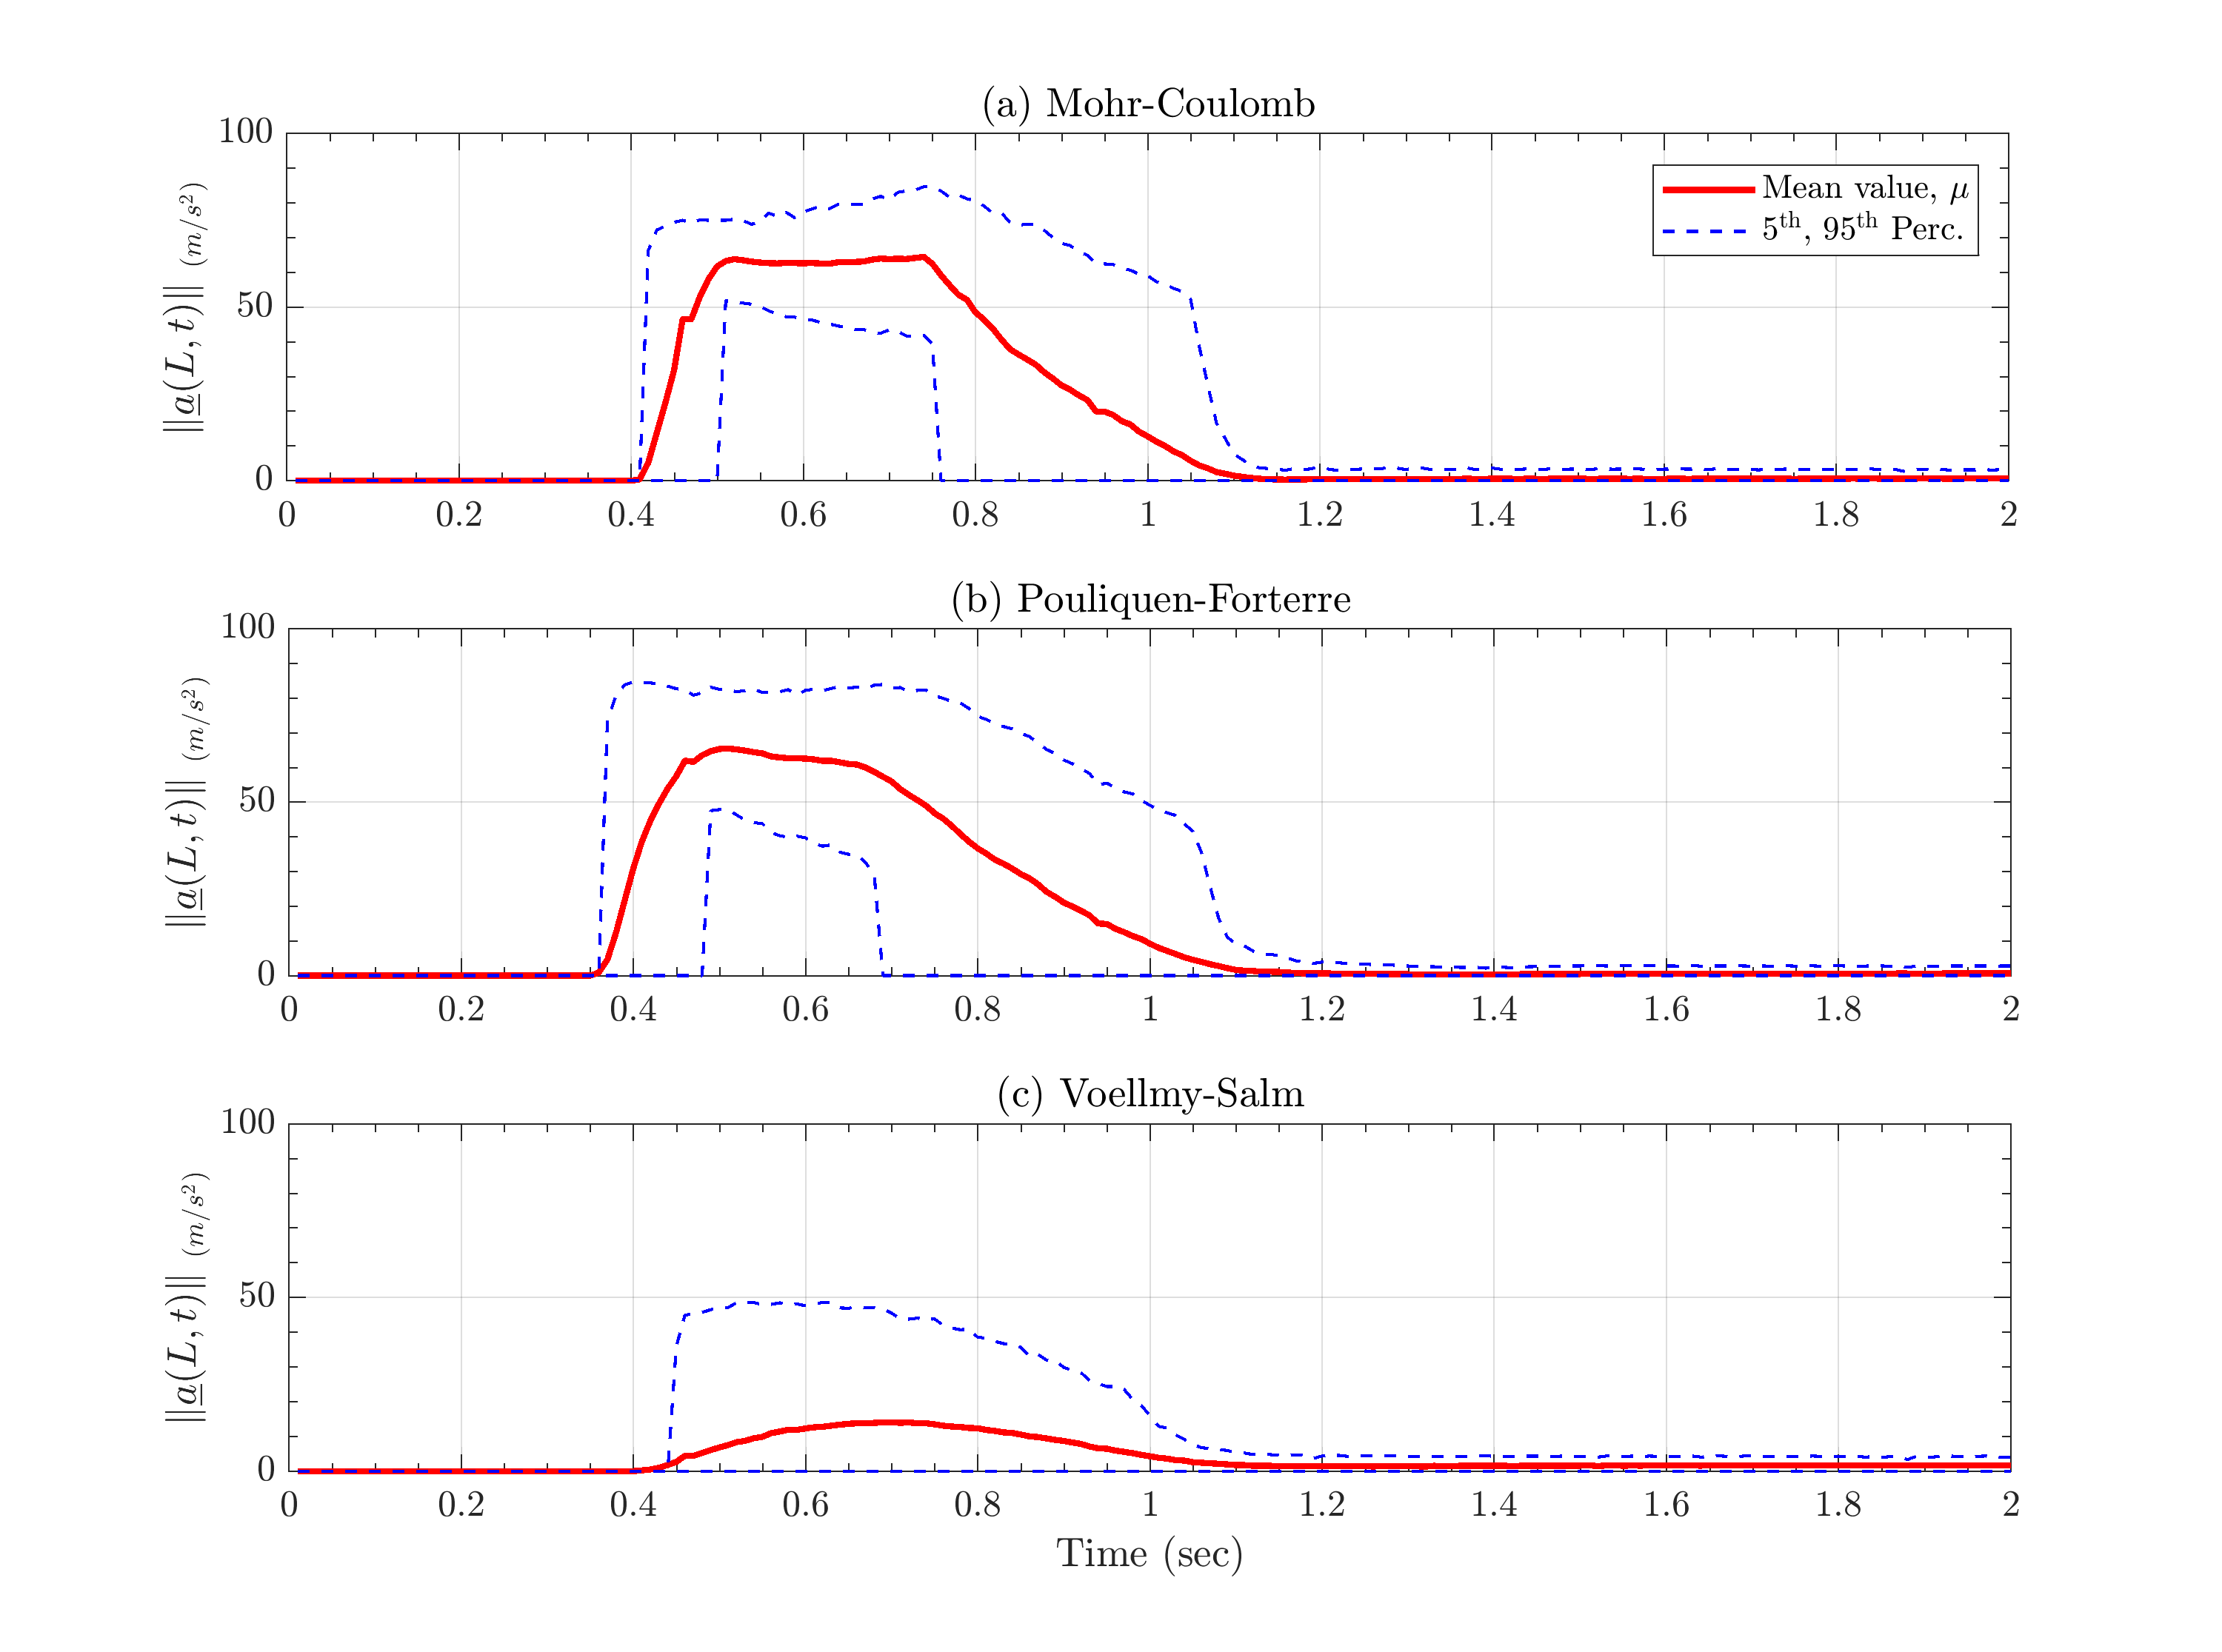
\includegraphics[width=1\textwidth]{InclinedPlane/Acceleration/accel_L3R.png}
    	\subcaption{$L=(0,0)$, inclined and runout planes' joint location.}
    	\label{fig:Ramp-L3-AccR}
	\end{minipage}
	\begin{minipage}[b]{0.5\linewidth}
		\centering
		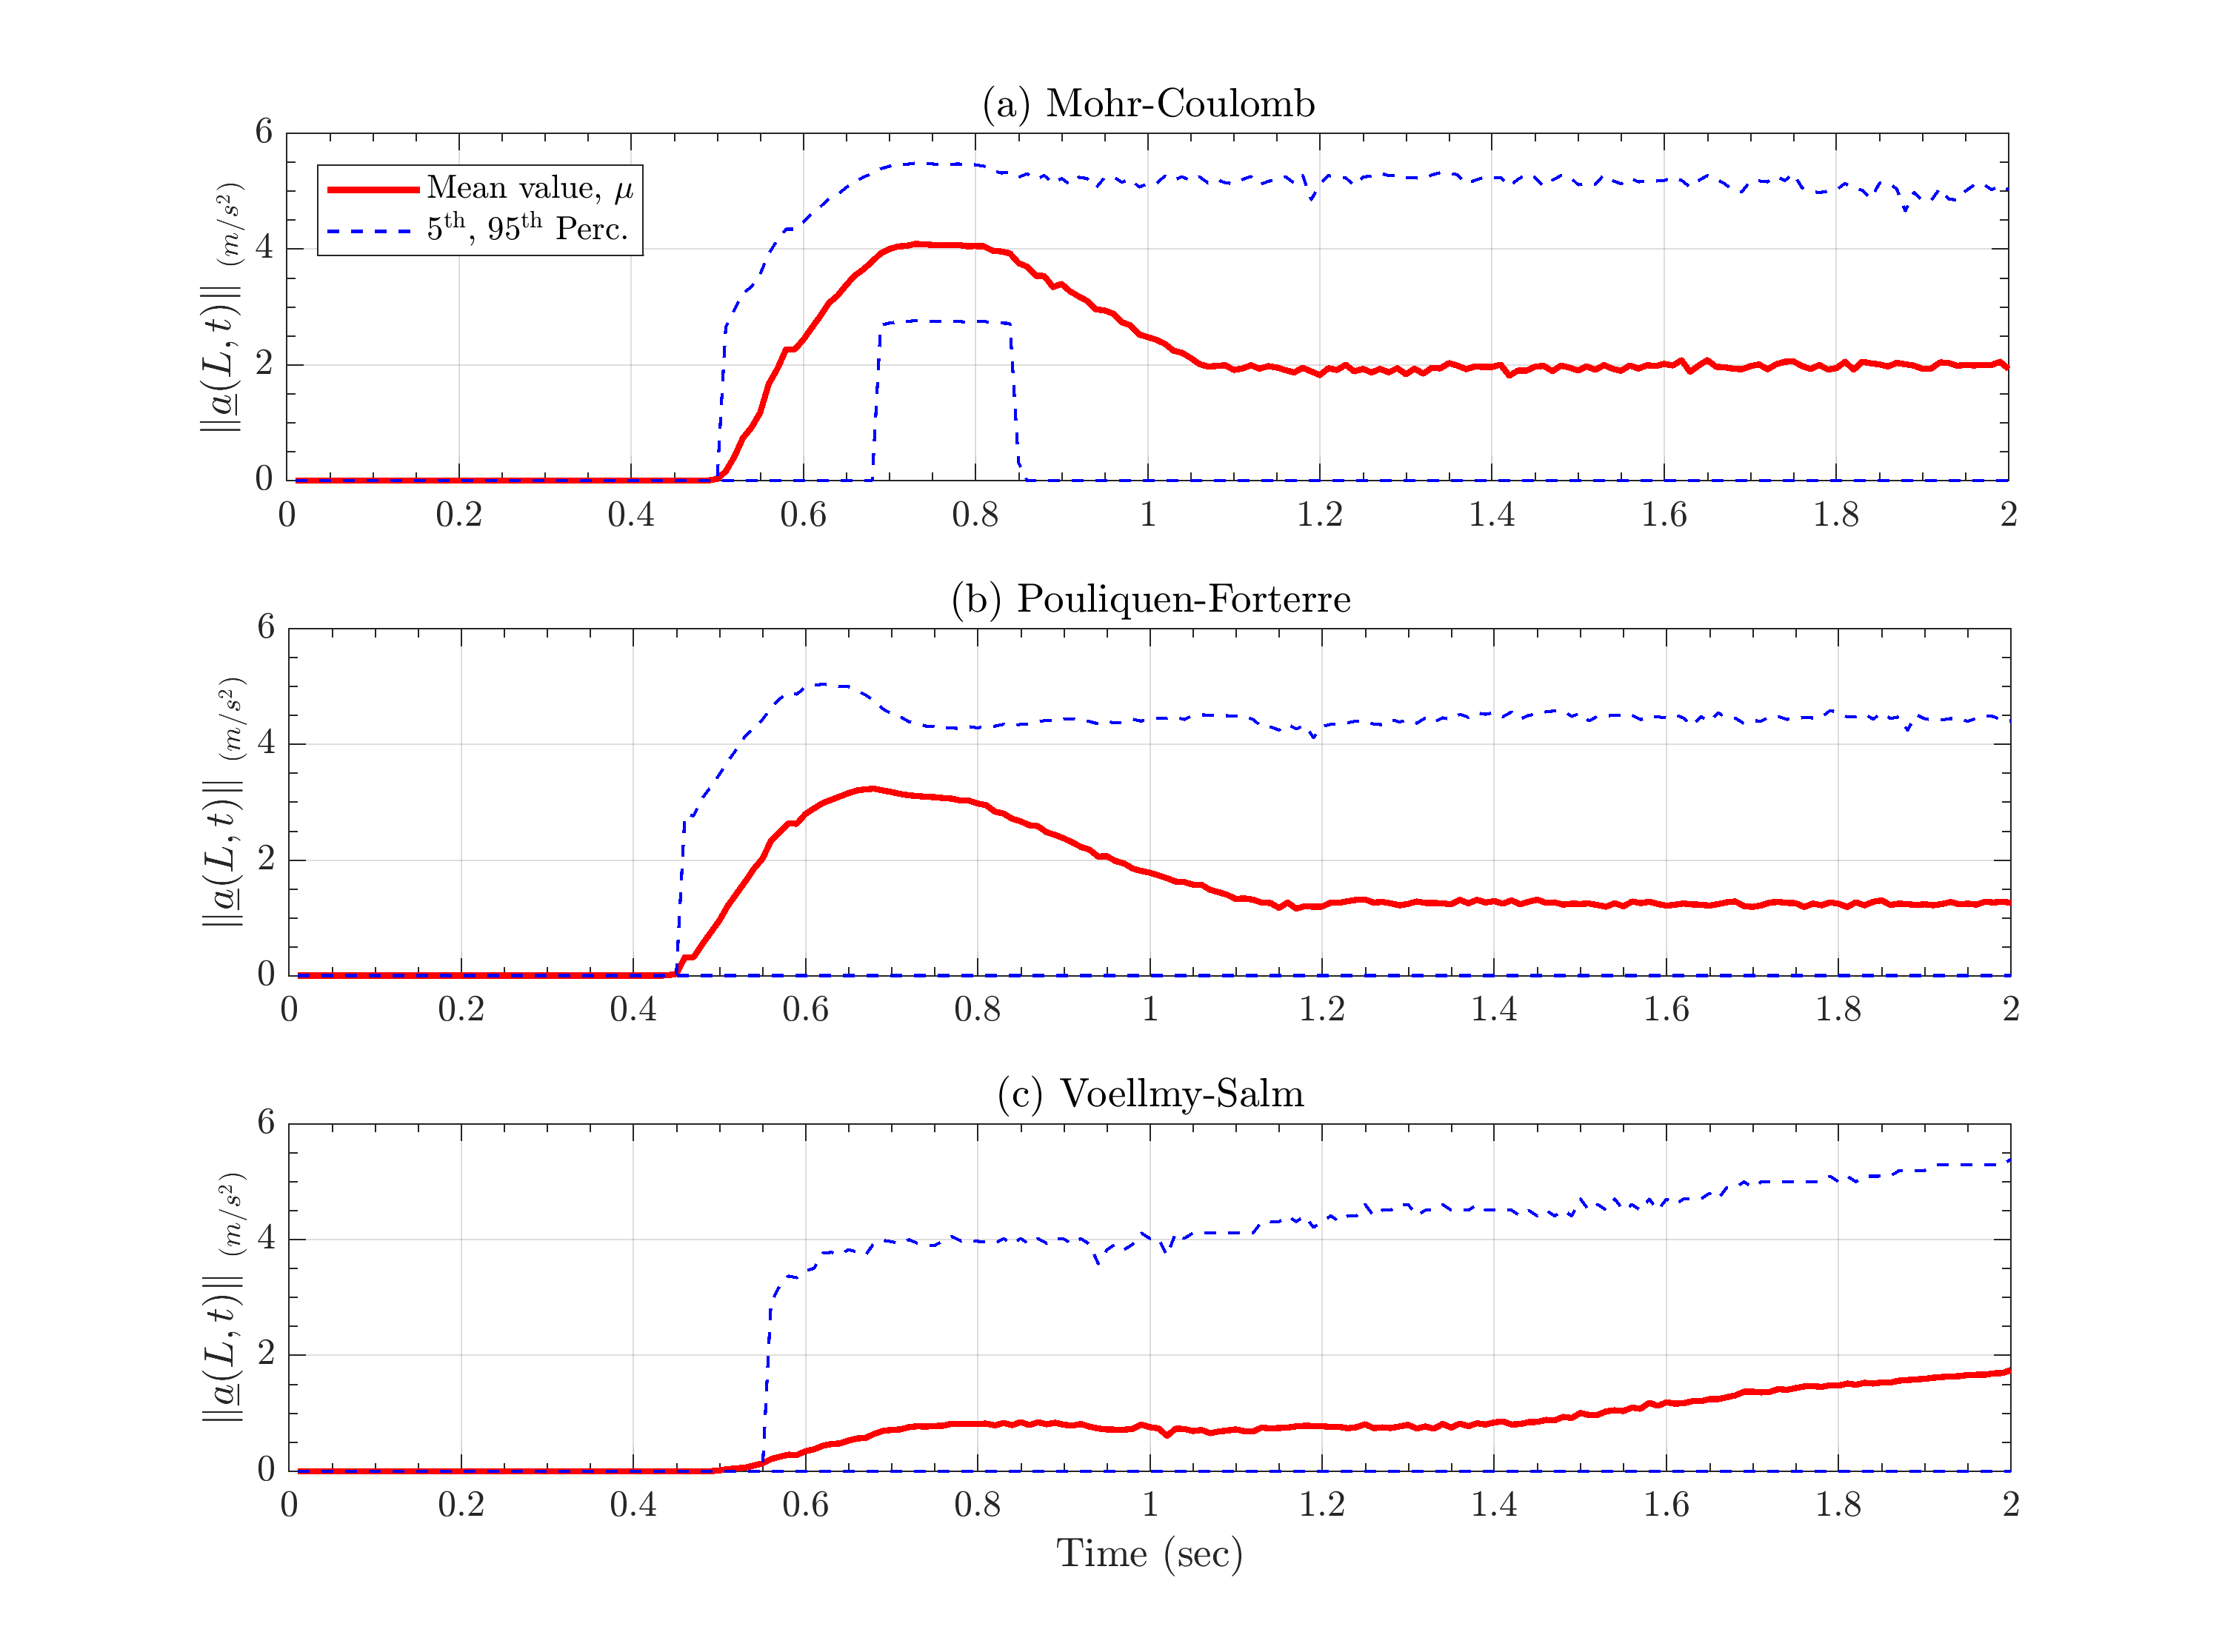
\includegraphics[width=1\textwidth]{InclinedPlane/Acceleration/accel_L4R.png}
    	\subcaption{$L=(0.15,0)$,  a location on runout plane.}
    	\label{fig:Ramp-L4-AccR}
    \end{minipage}
    \caption{Records of flow acceleration (computed from RHS), $\Vert \underline{\mathbf{a}} \Vert(L,t)$.}
    \label{fig:Ramp-LM-AccR}
\end{figure}

\begin{figure}[H]
        \centering
        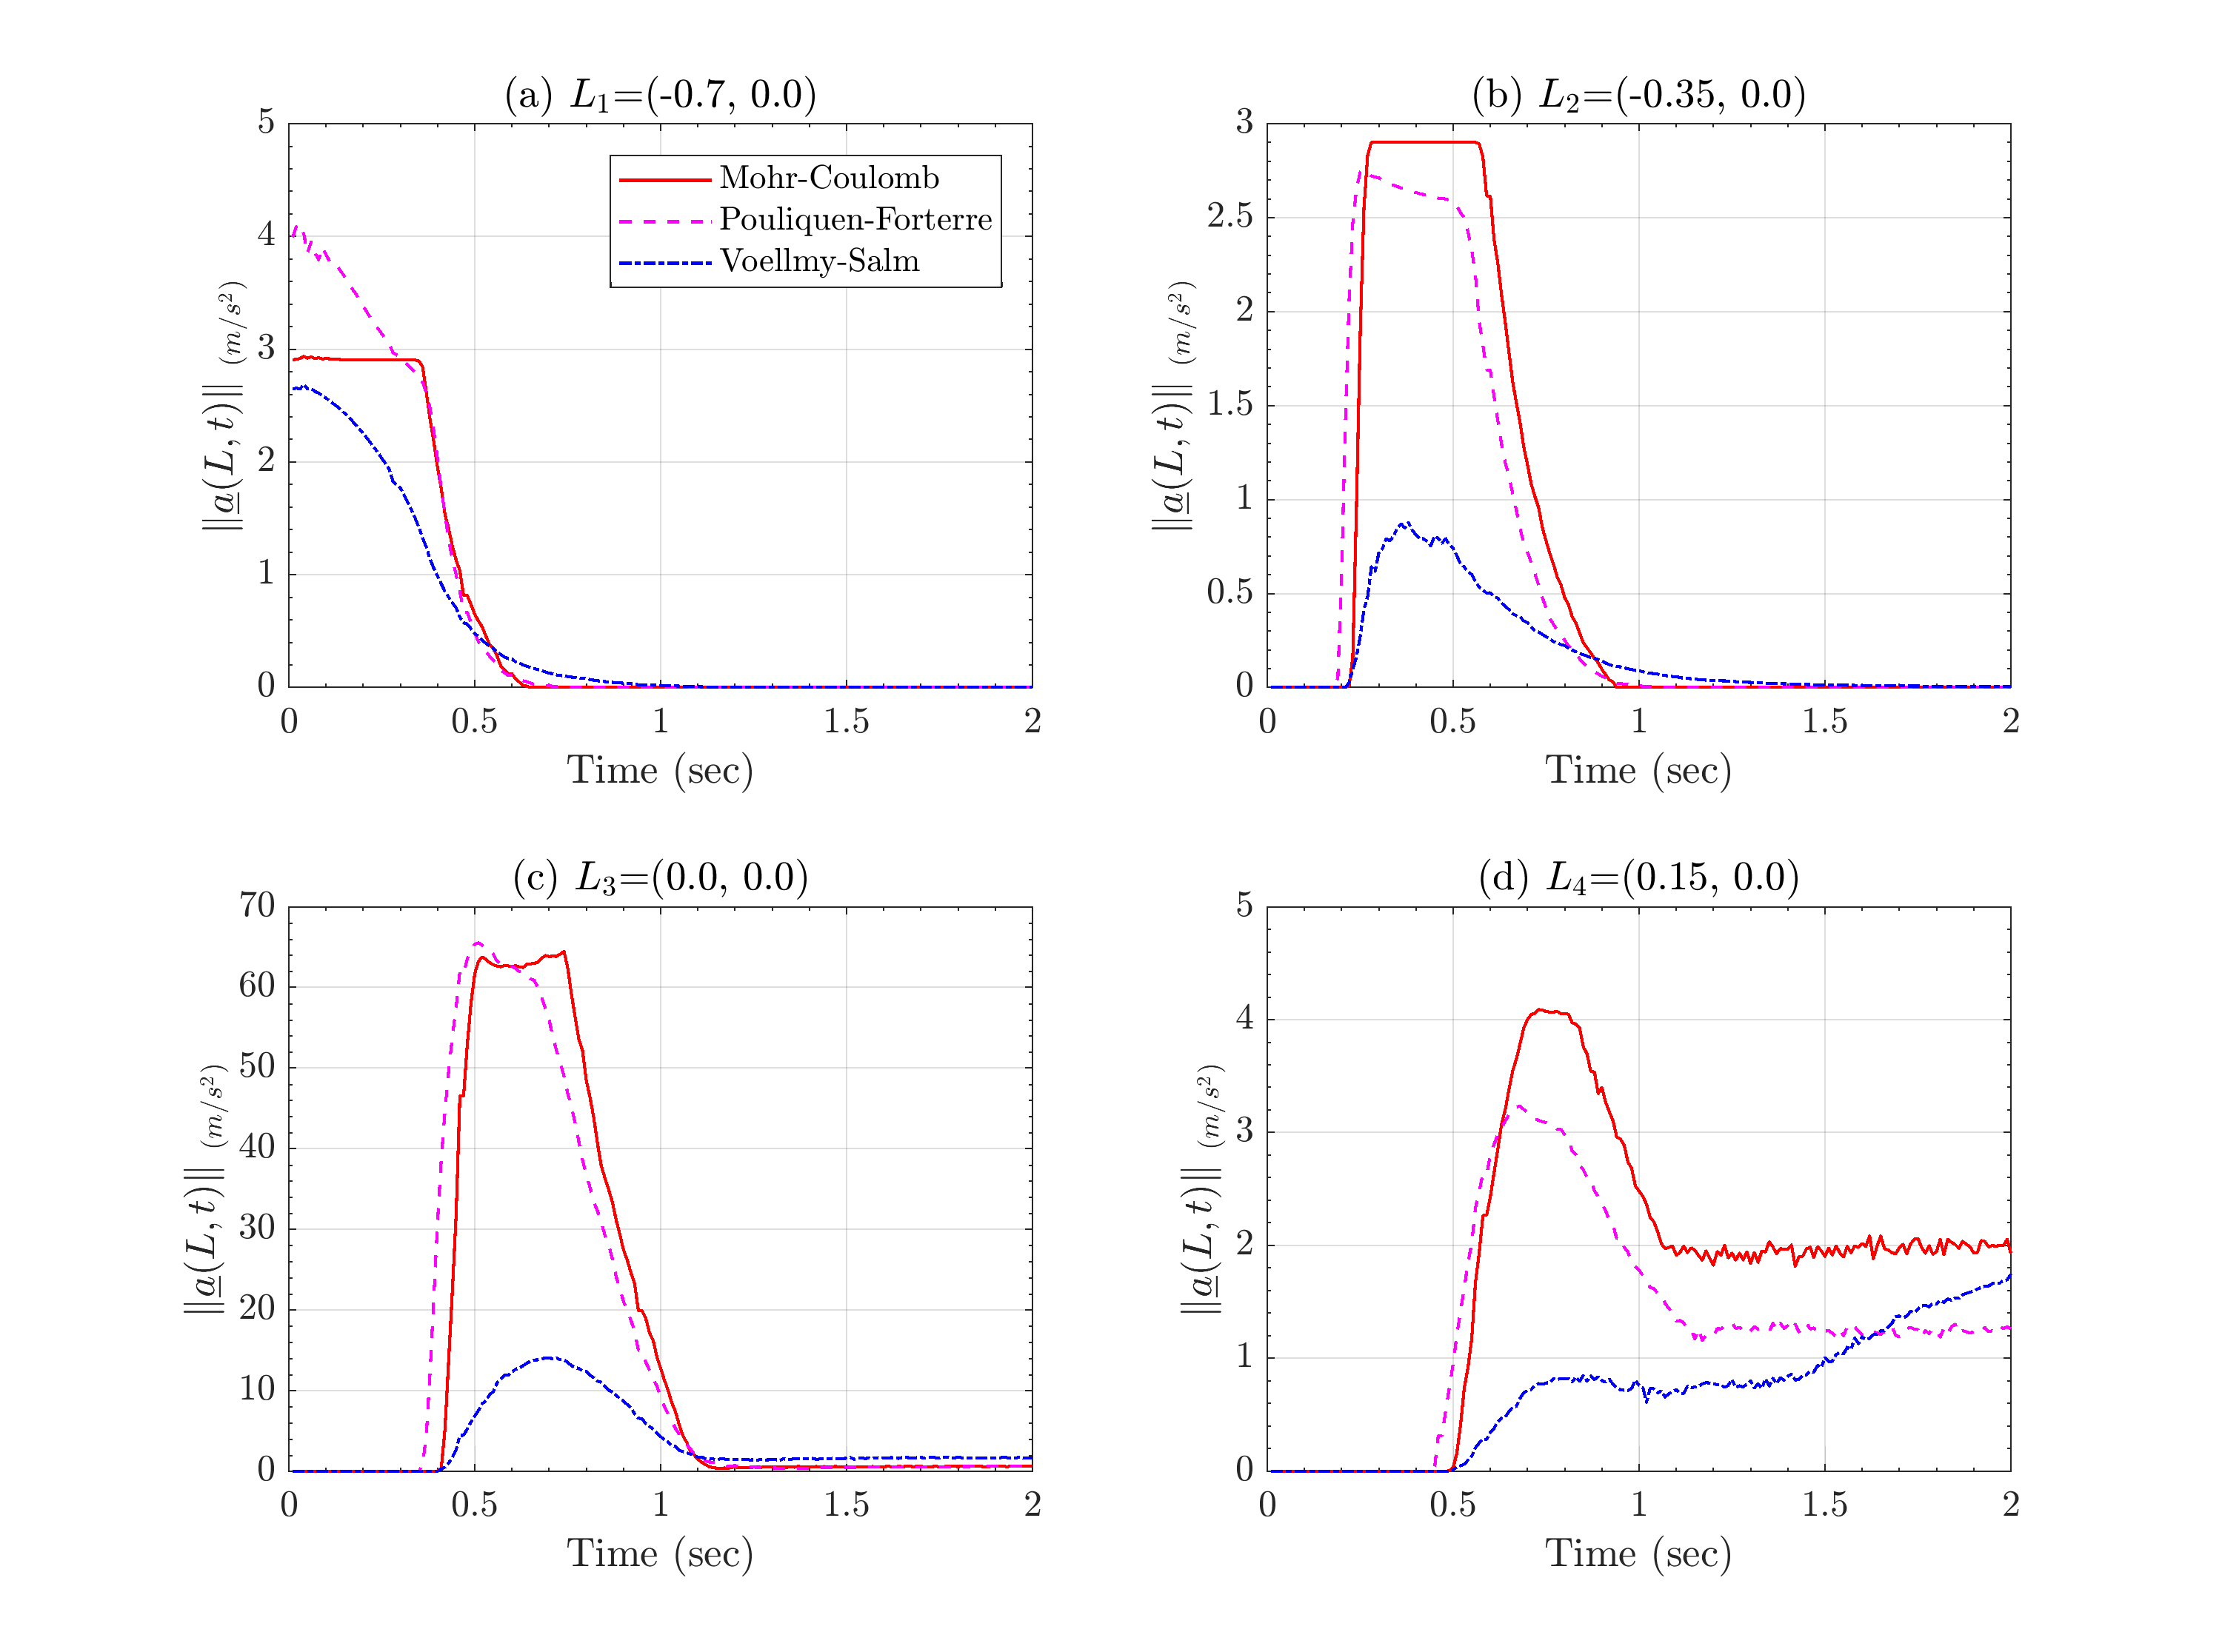
\includegraphics[width=1\textwidth]{InclinedPlane/Acceleration/accel_meanR.png}
        \caption{Comparison between mean values of flow acceleration (computed from RHS), $\Vert \underline{a} \Vert(L,t)$, recorded at locations of interest, $L_i, \ _{i=1,...,4}$.}
        \label{fig:Ramp-LM-AccR-means}
\end{figure}


\begin{figure}[H]
	\begin{minipage}[b]{0.5\linewidth}
    	\centering
    	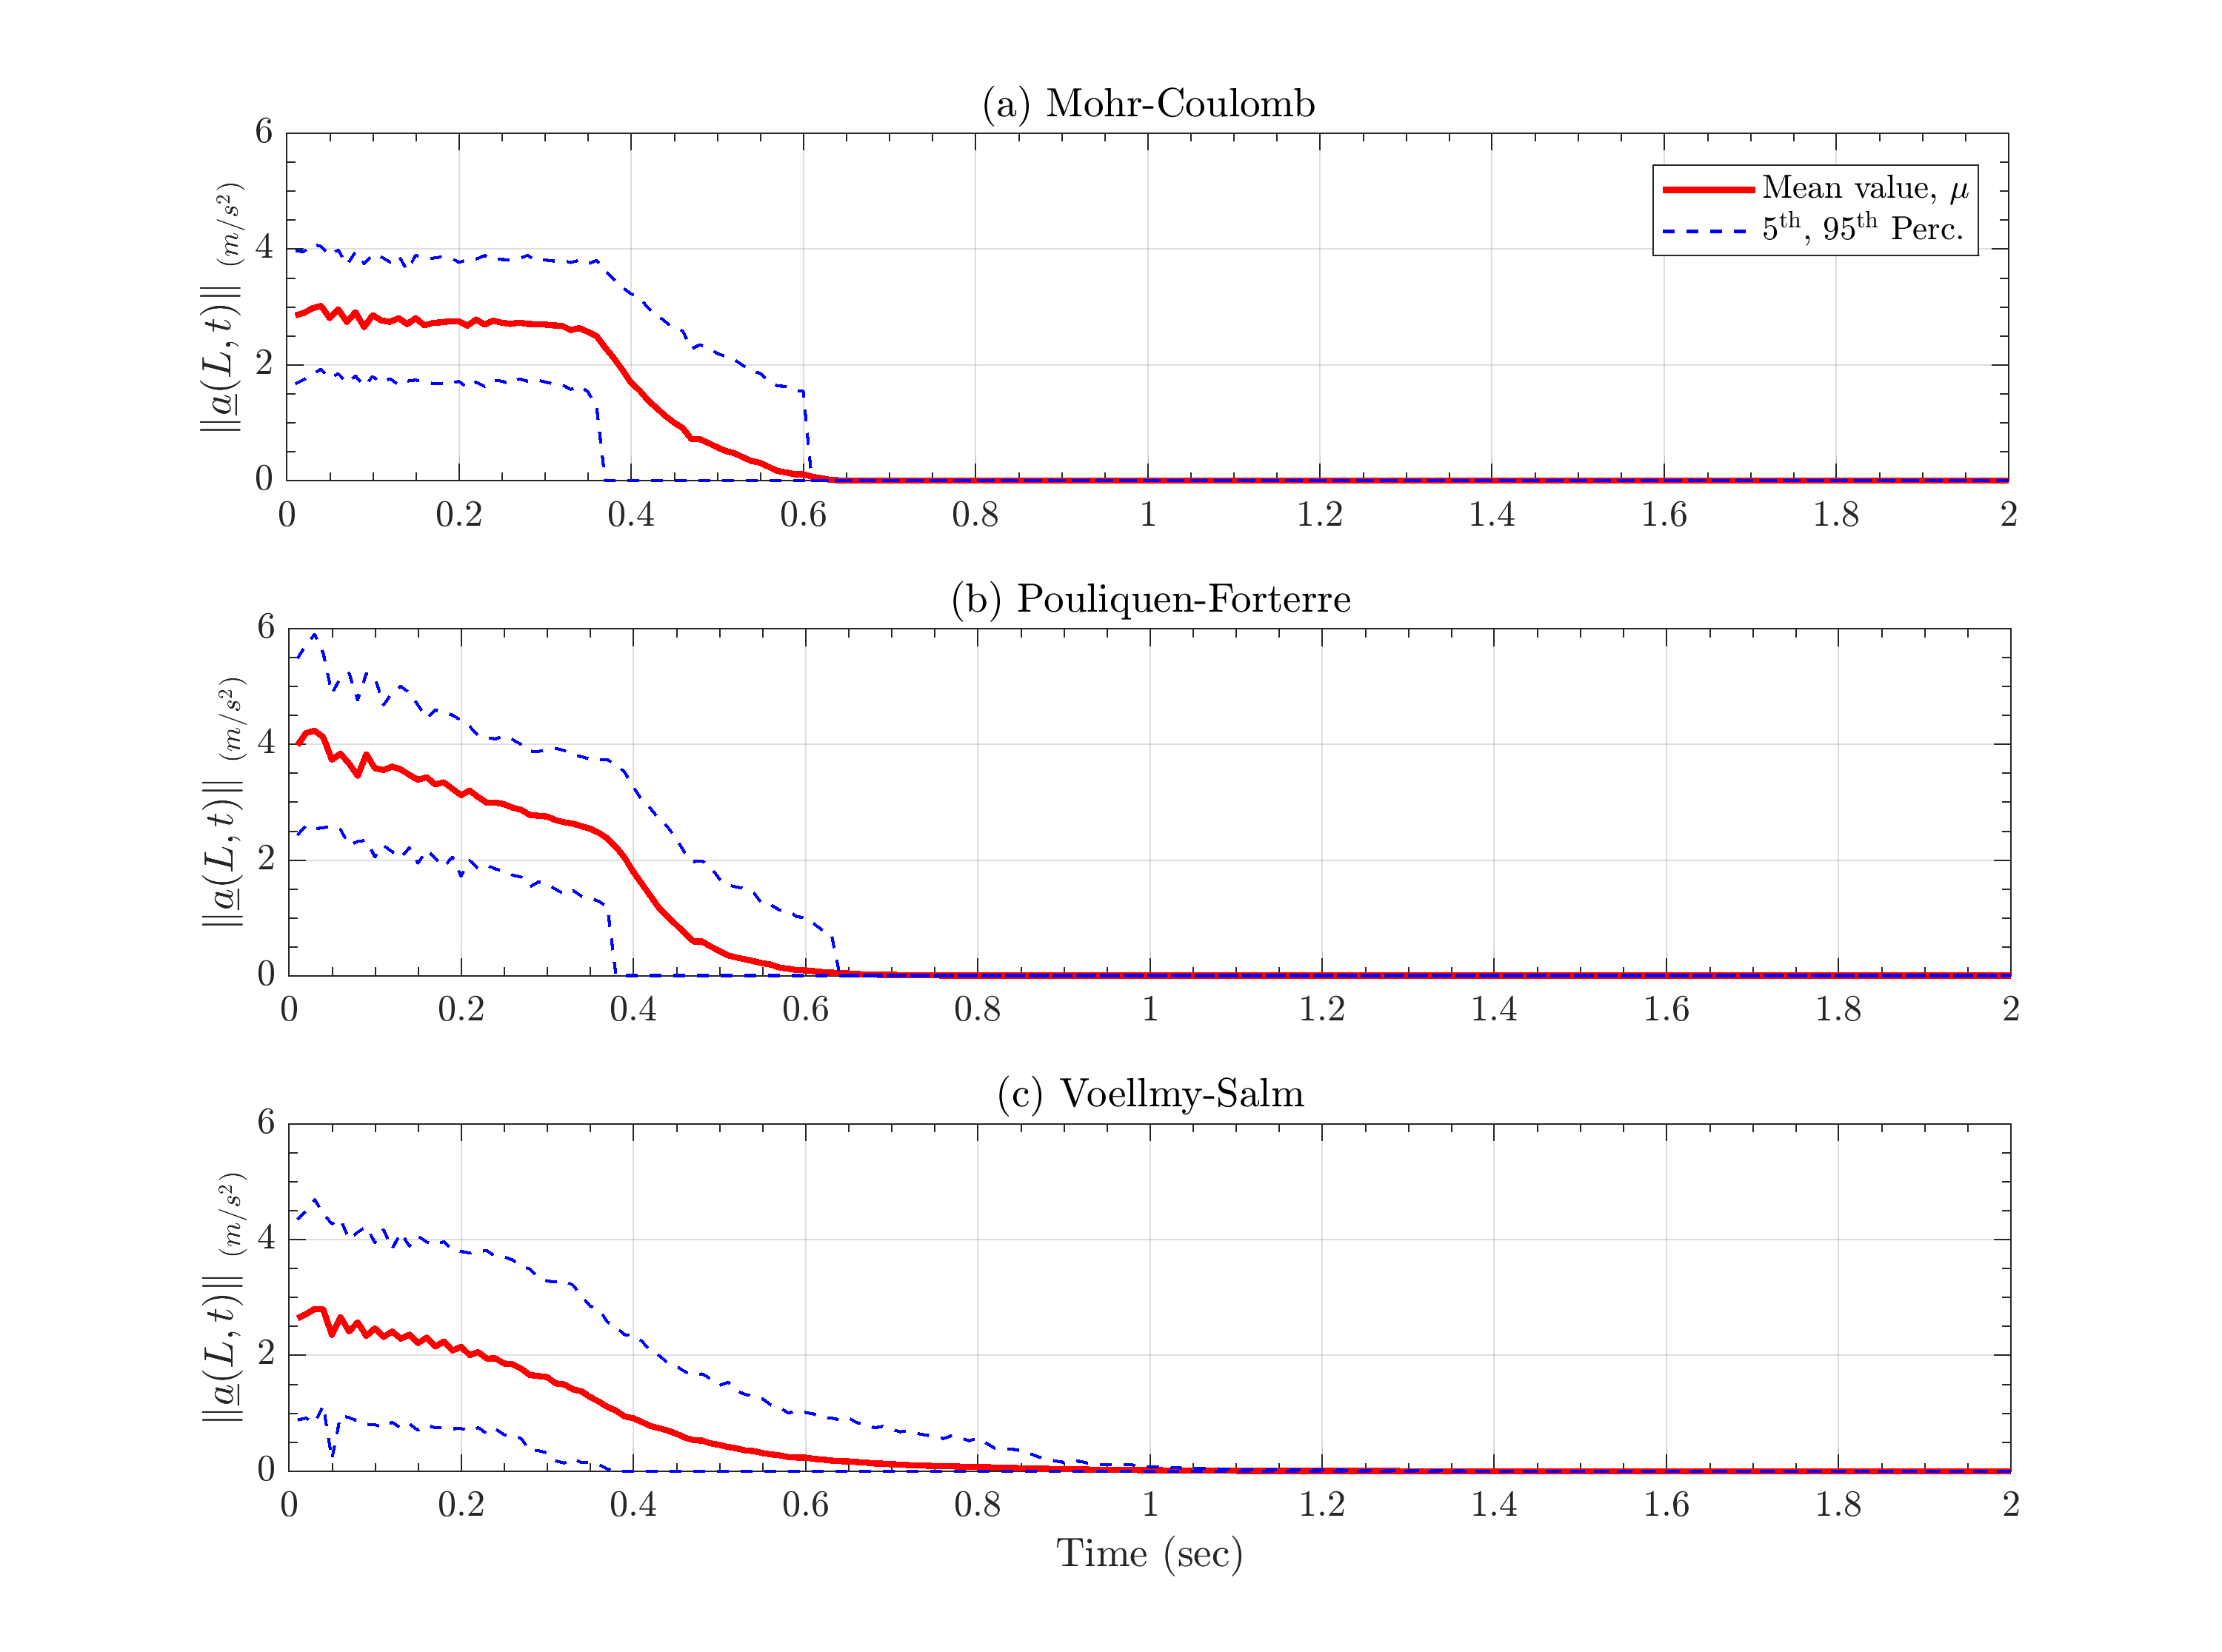
\includegraphics[width=1\textwidth]{InclinedPlane/Acceleration/accel_L1L.png}
    	\subcaption{$L=(-0.7,0)$, slumping pile location.}
    	\label{fig:Ramp-L1-AccL}
	\end{minipage}
	\begin{minipage}[b]{0.5\linewidth}
		\centering
		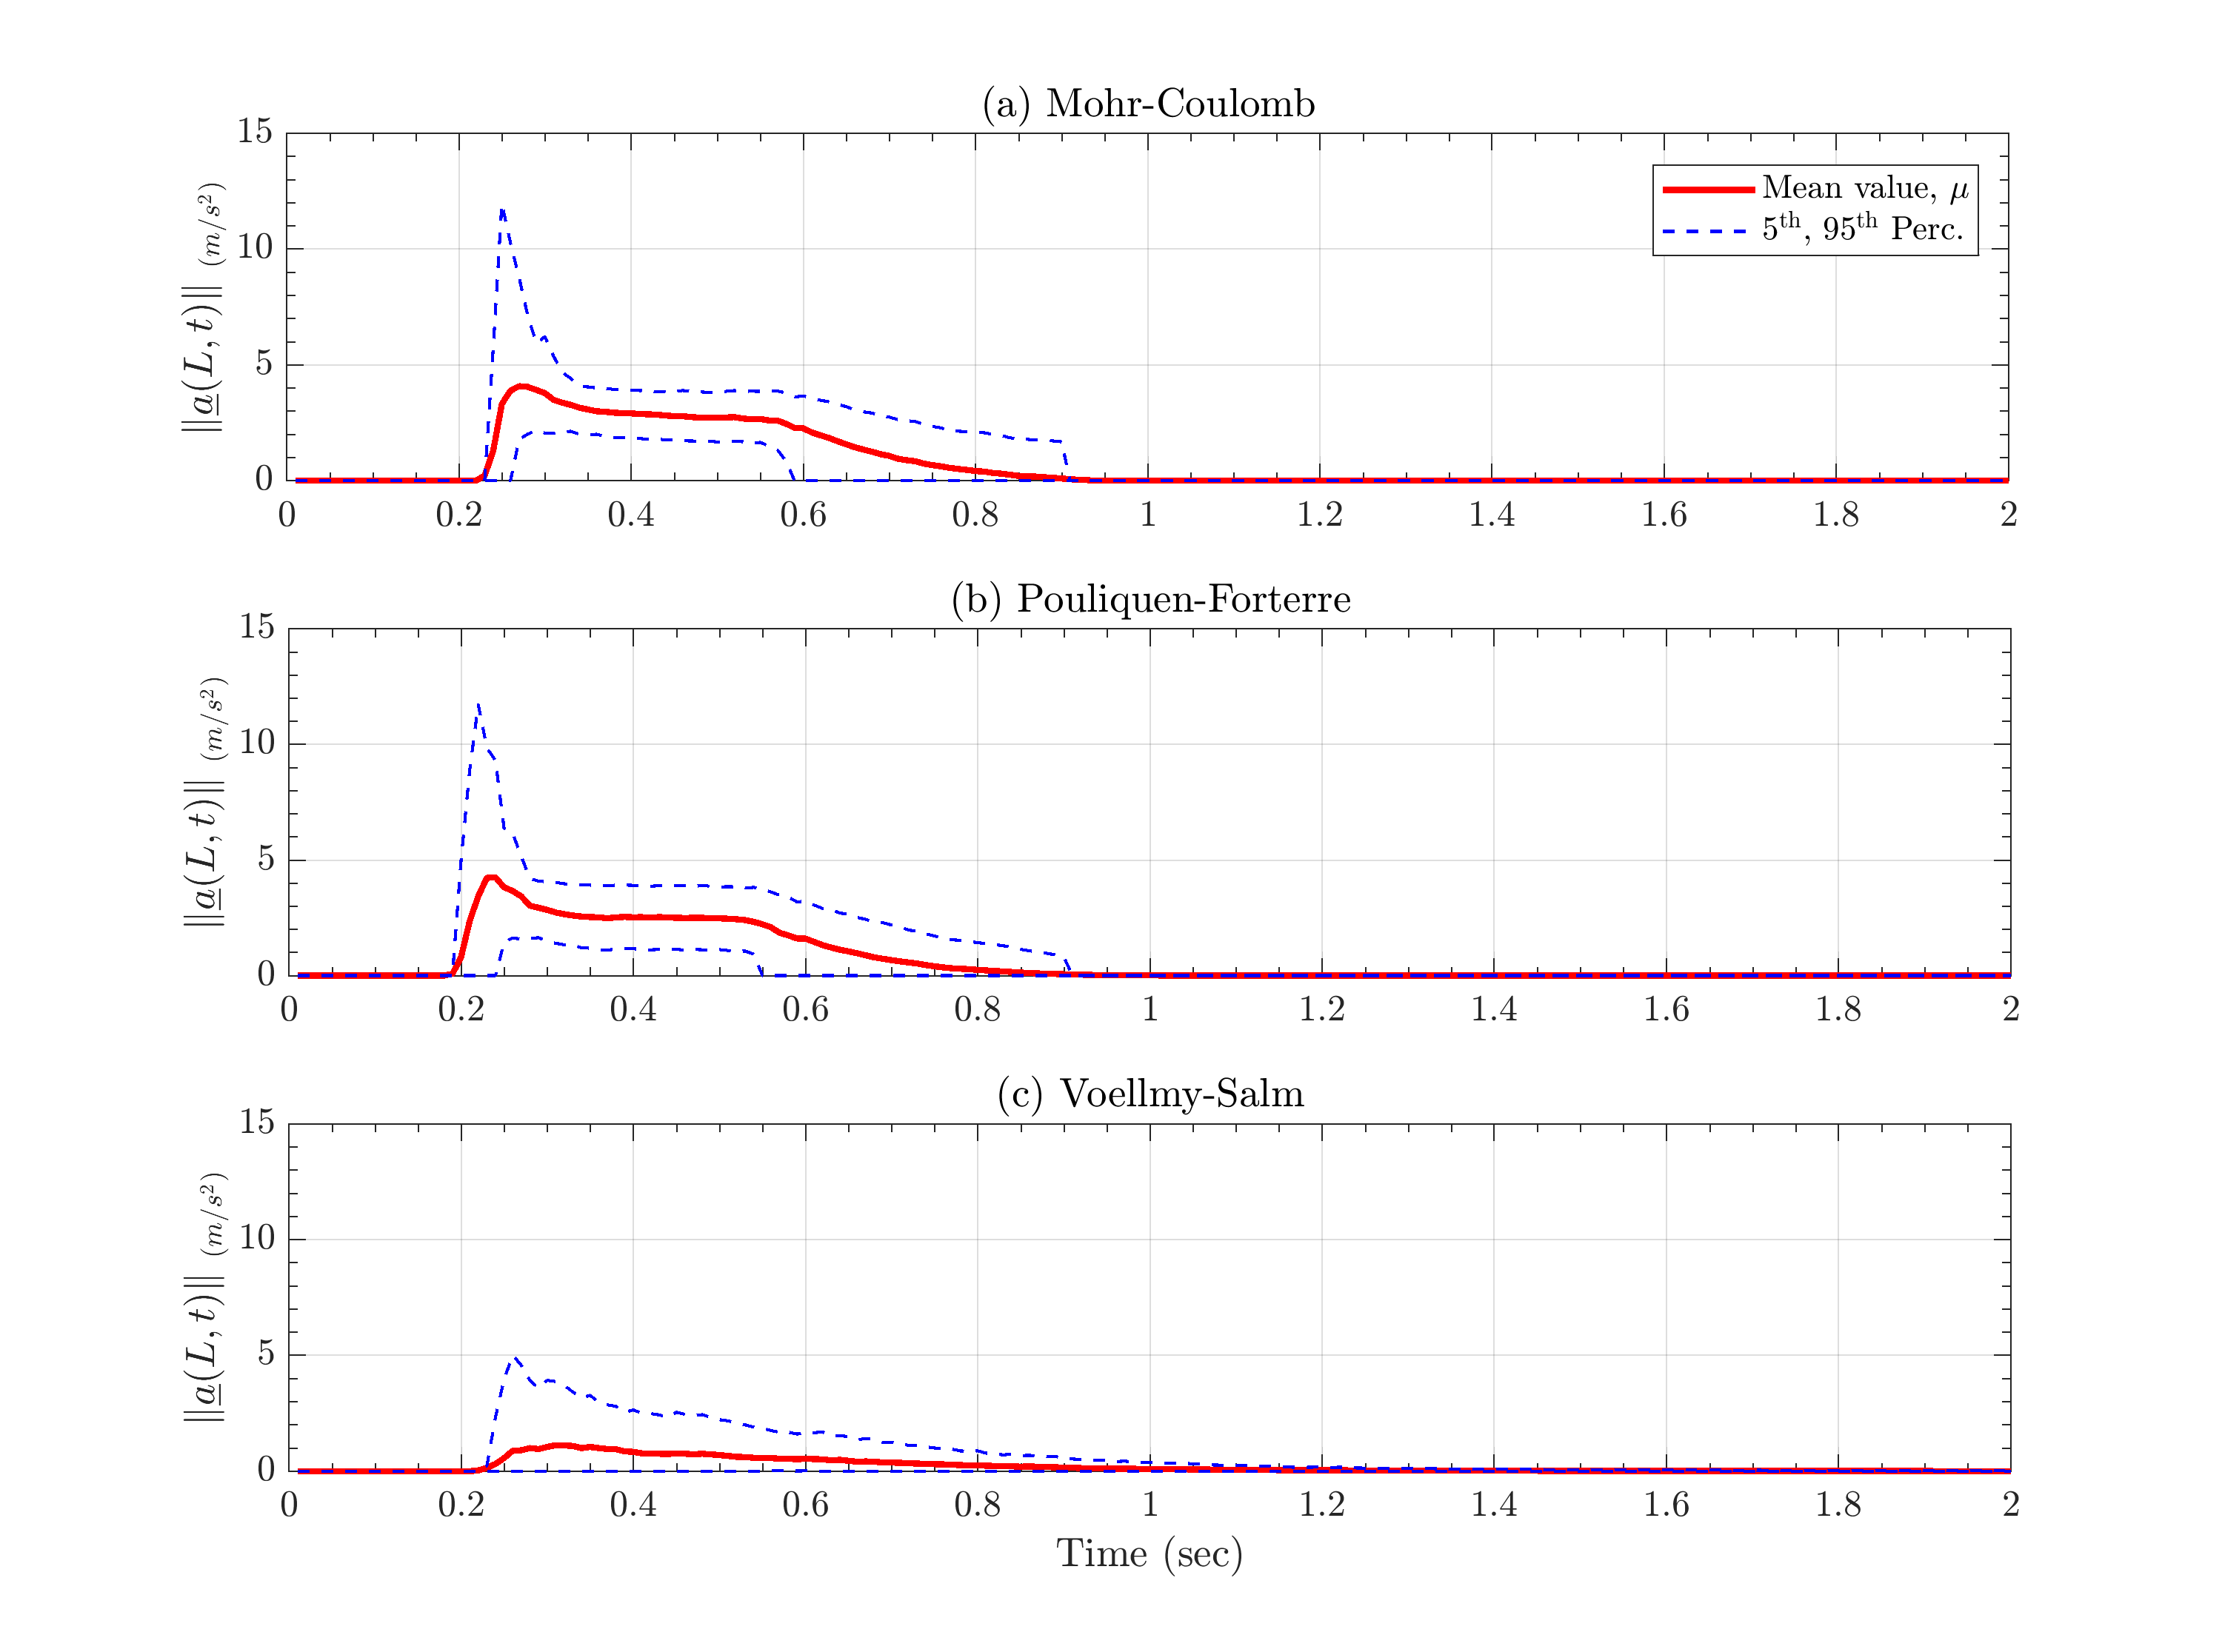
\includegraphics[width=1\textwidth]{InclinedPlane/Acceleration/accel_L2L.png}
    	\subcaption{$L=(-0.35,0)$, middle point on inclined plane.}
    	\label{fig:Ramp-L2-AccL}
    \end{minipage}

	\begin{minipage}[b]{0.5\linewidth}
    	\centering
    	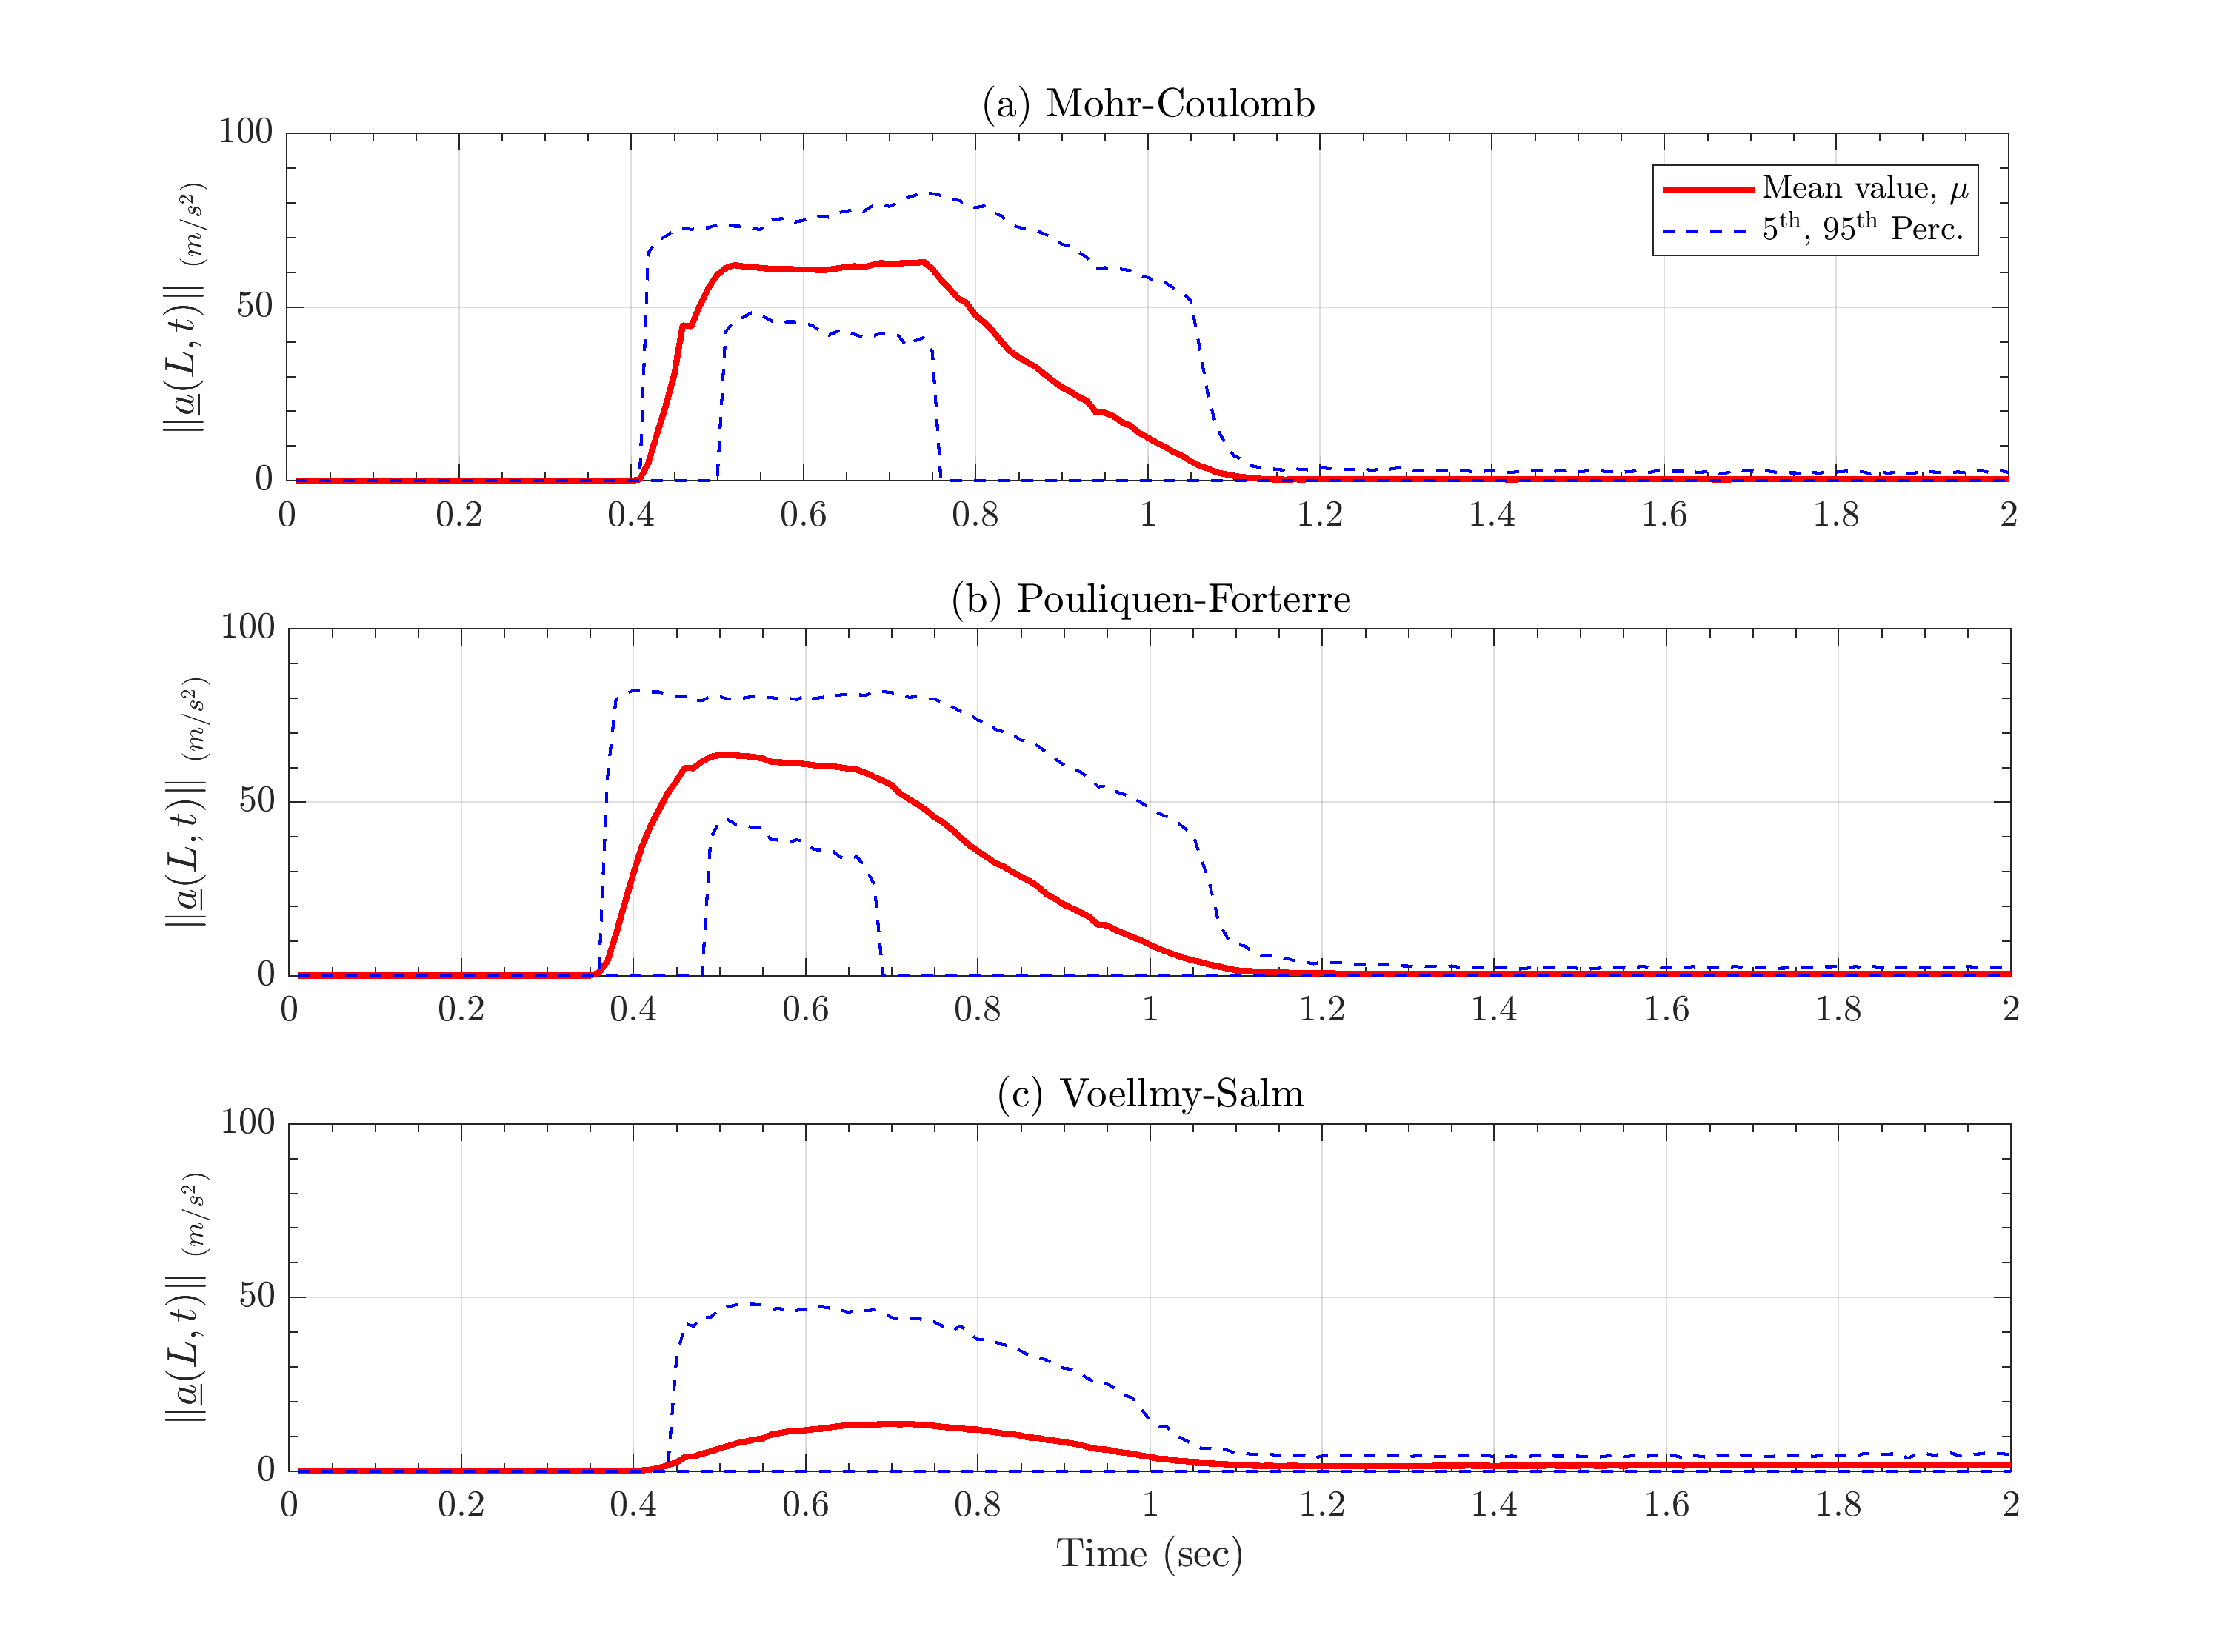
\includegraphics[width=1\textwidth]{InclinedPlane/Acceleration/accel_L3L.png}
    	\subcaption{$L=(0,0)$, inclined and runout planes' joint location.}
    	\label{fig:Ramp-L3-AccL}
	\end{minipage}
	\begin{minipage}[b]{0.5\linewidth}
		\centering
		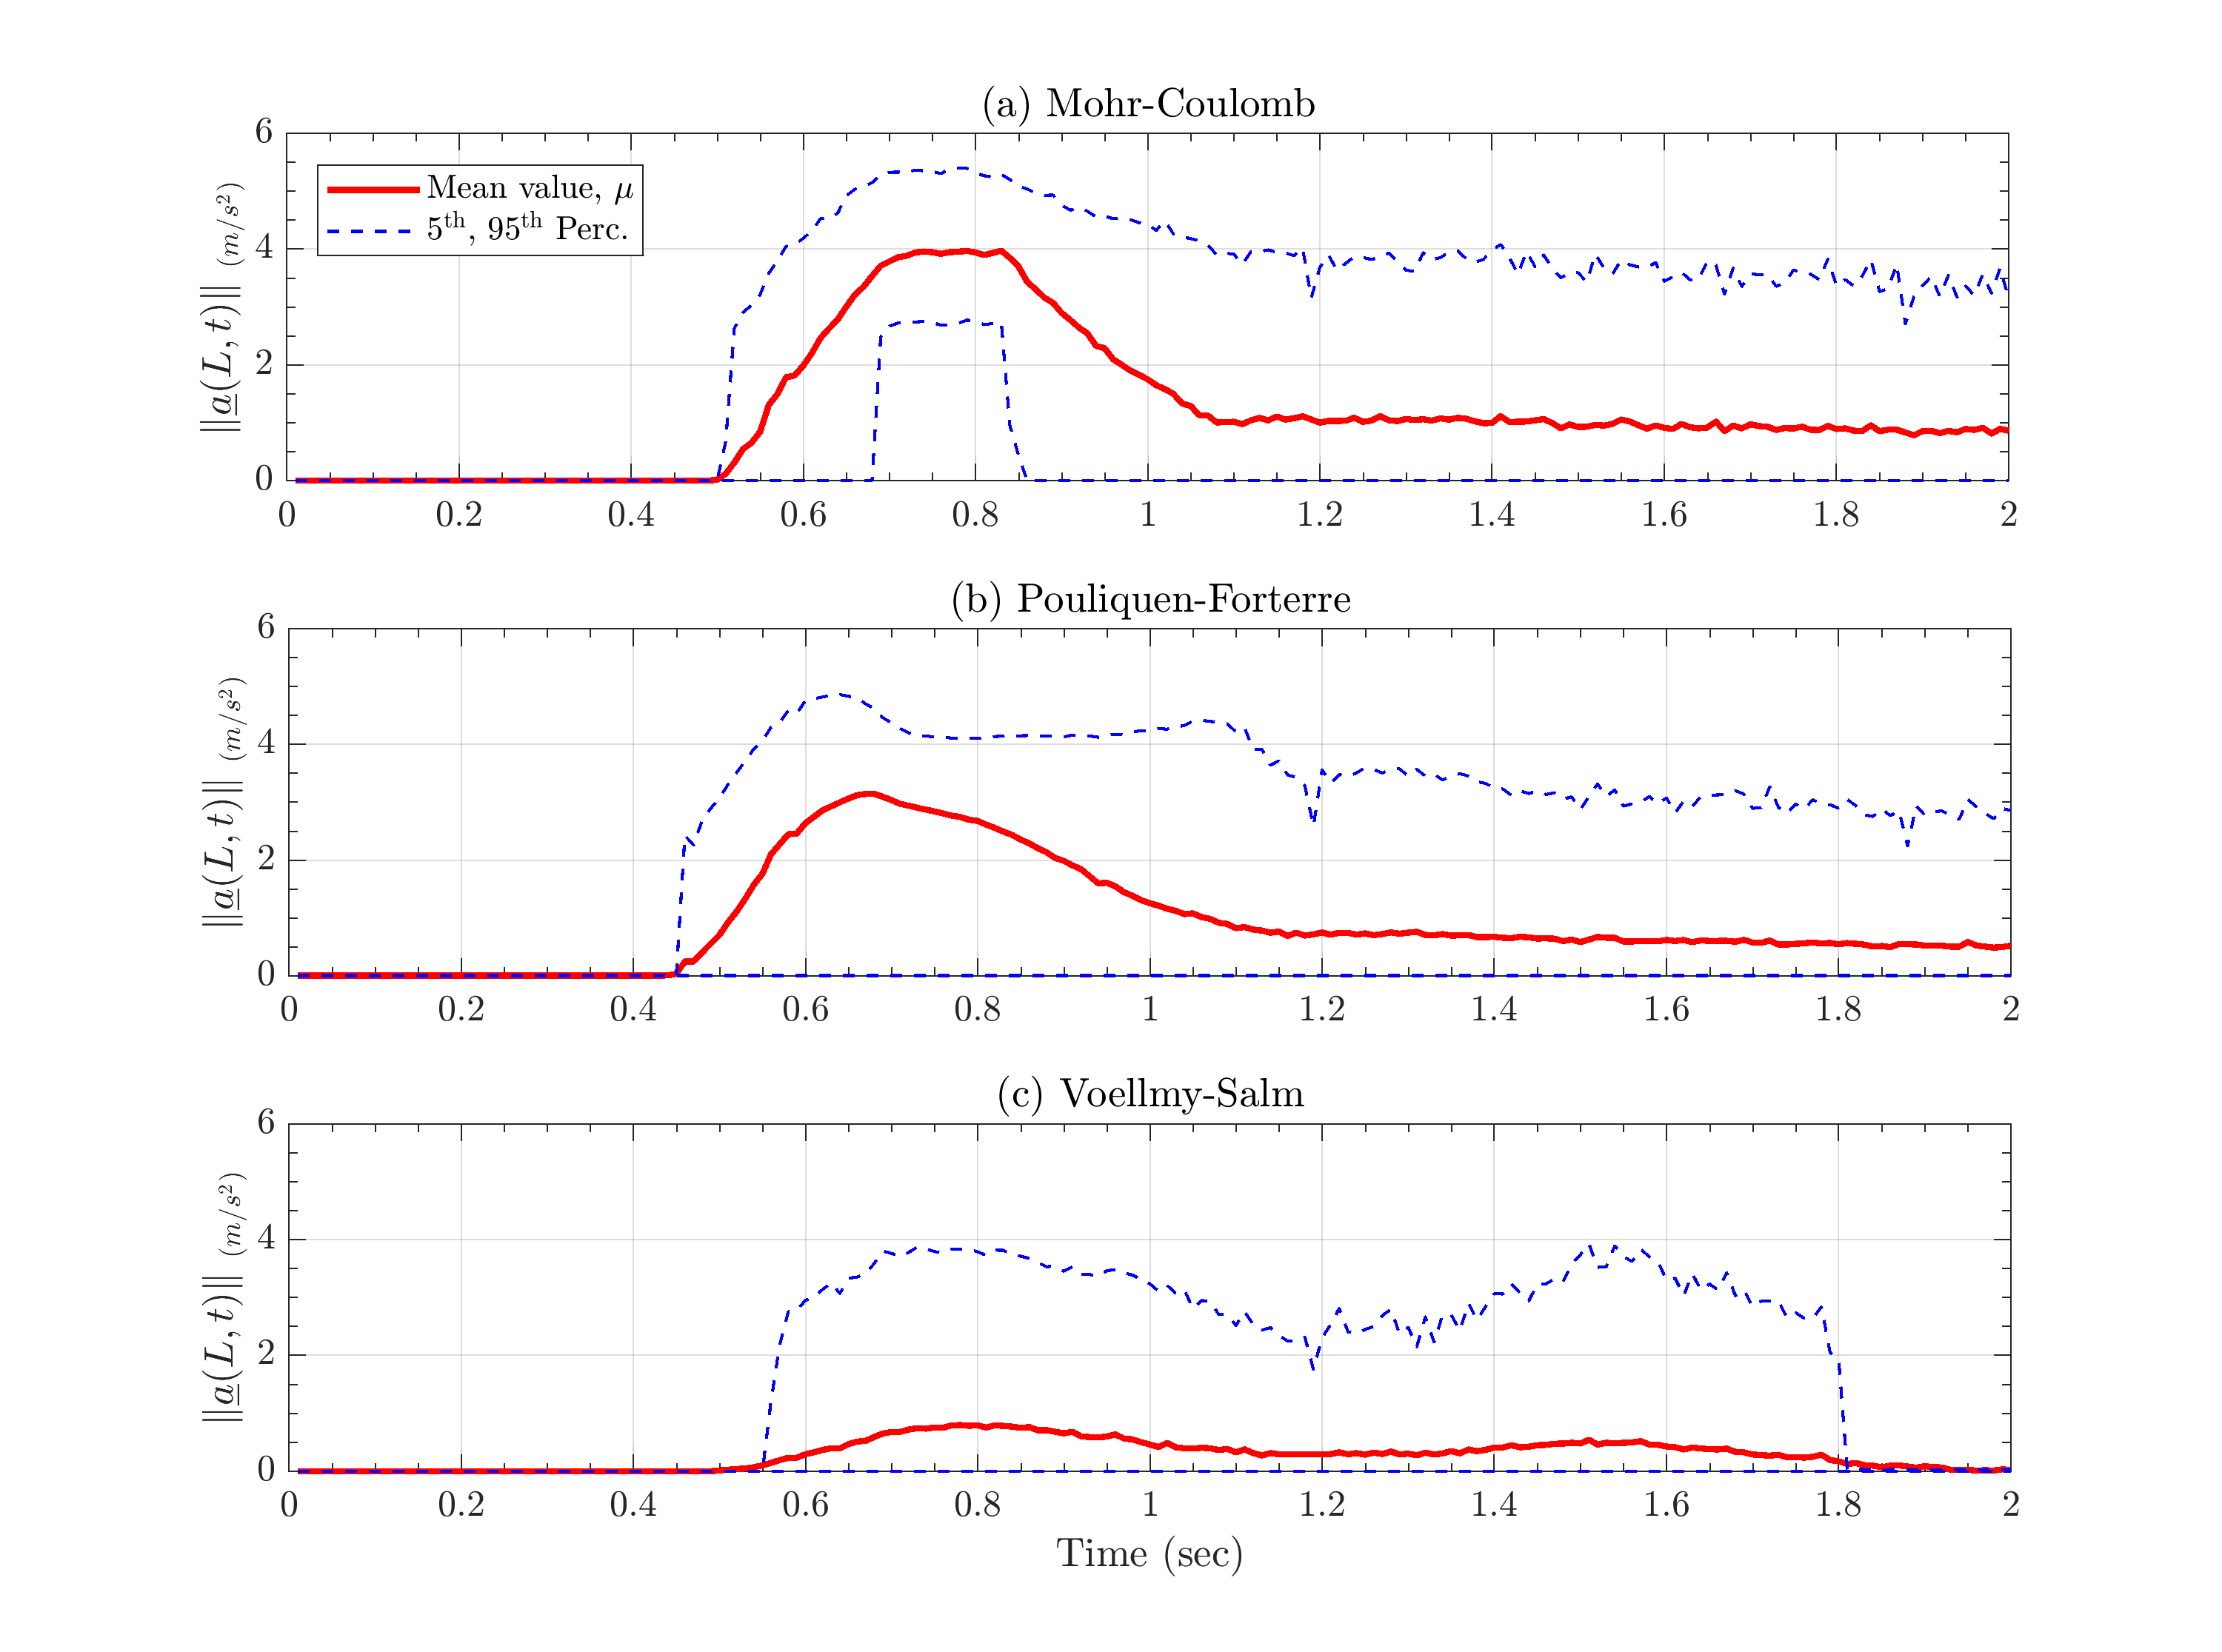
\includegraphics[width=1\textwidth]{InclinedPlane/Acceleration/accel_L4L.png}
    	\subcaption{$L=(0.15,0)$,  a location on runout plane.}
    	\label{fig:Ramp-L4-AccL}
    \end{minipage}
    \caption{Records of flow acceleration (computed from LHS), $\Vert \underline{\mathbf{a}} \Vert(L,t)$.}
    \label{fig:Ramp-LM-AccL}
\end{figure}

\begin{figure}[H]
        \centering
        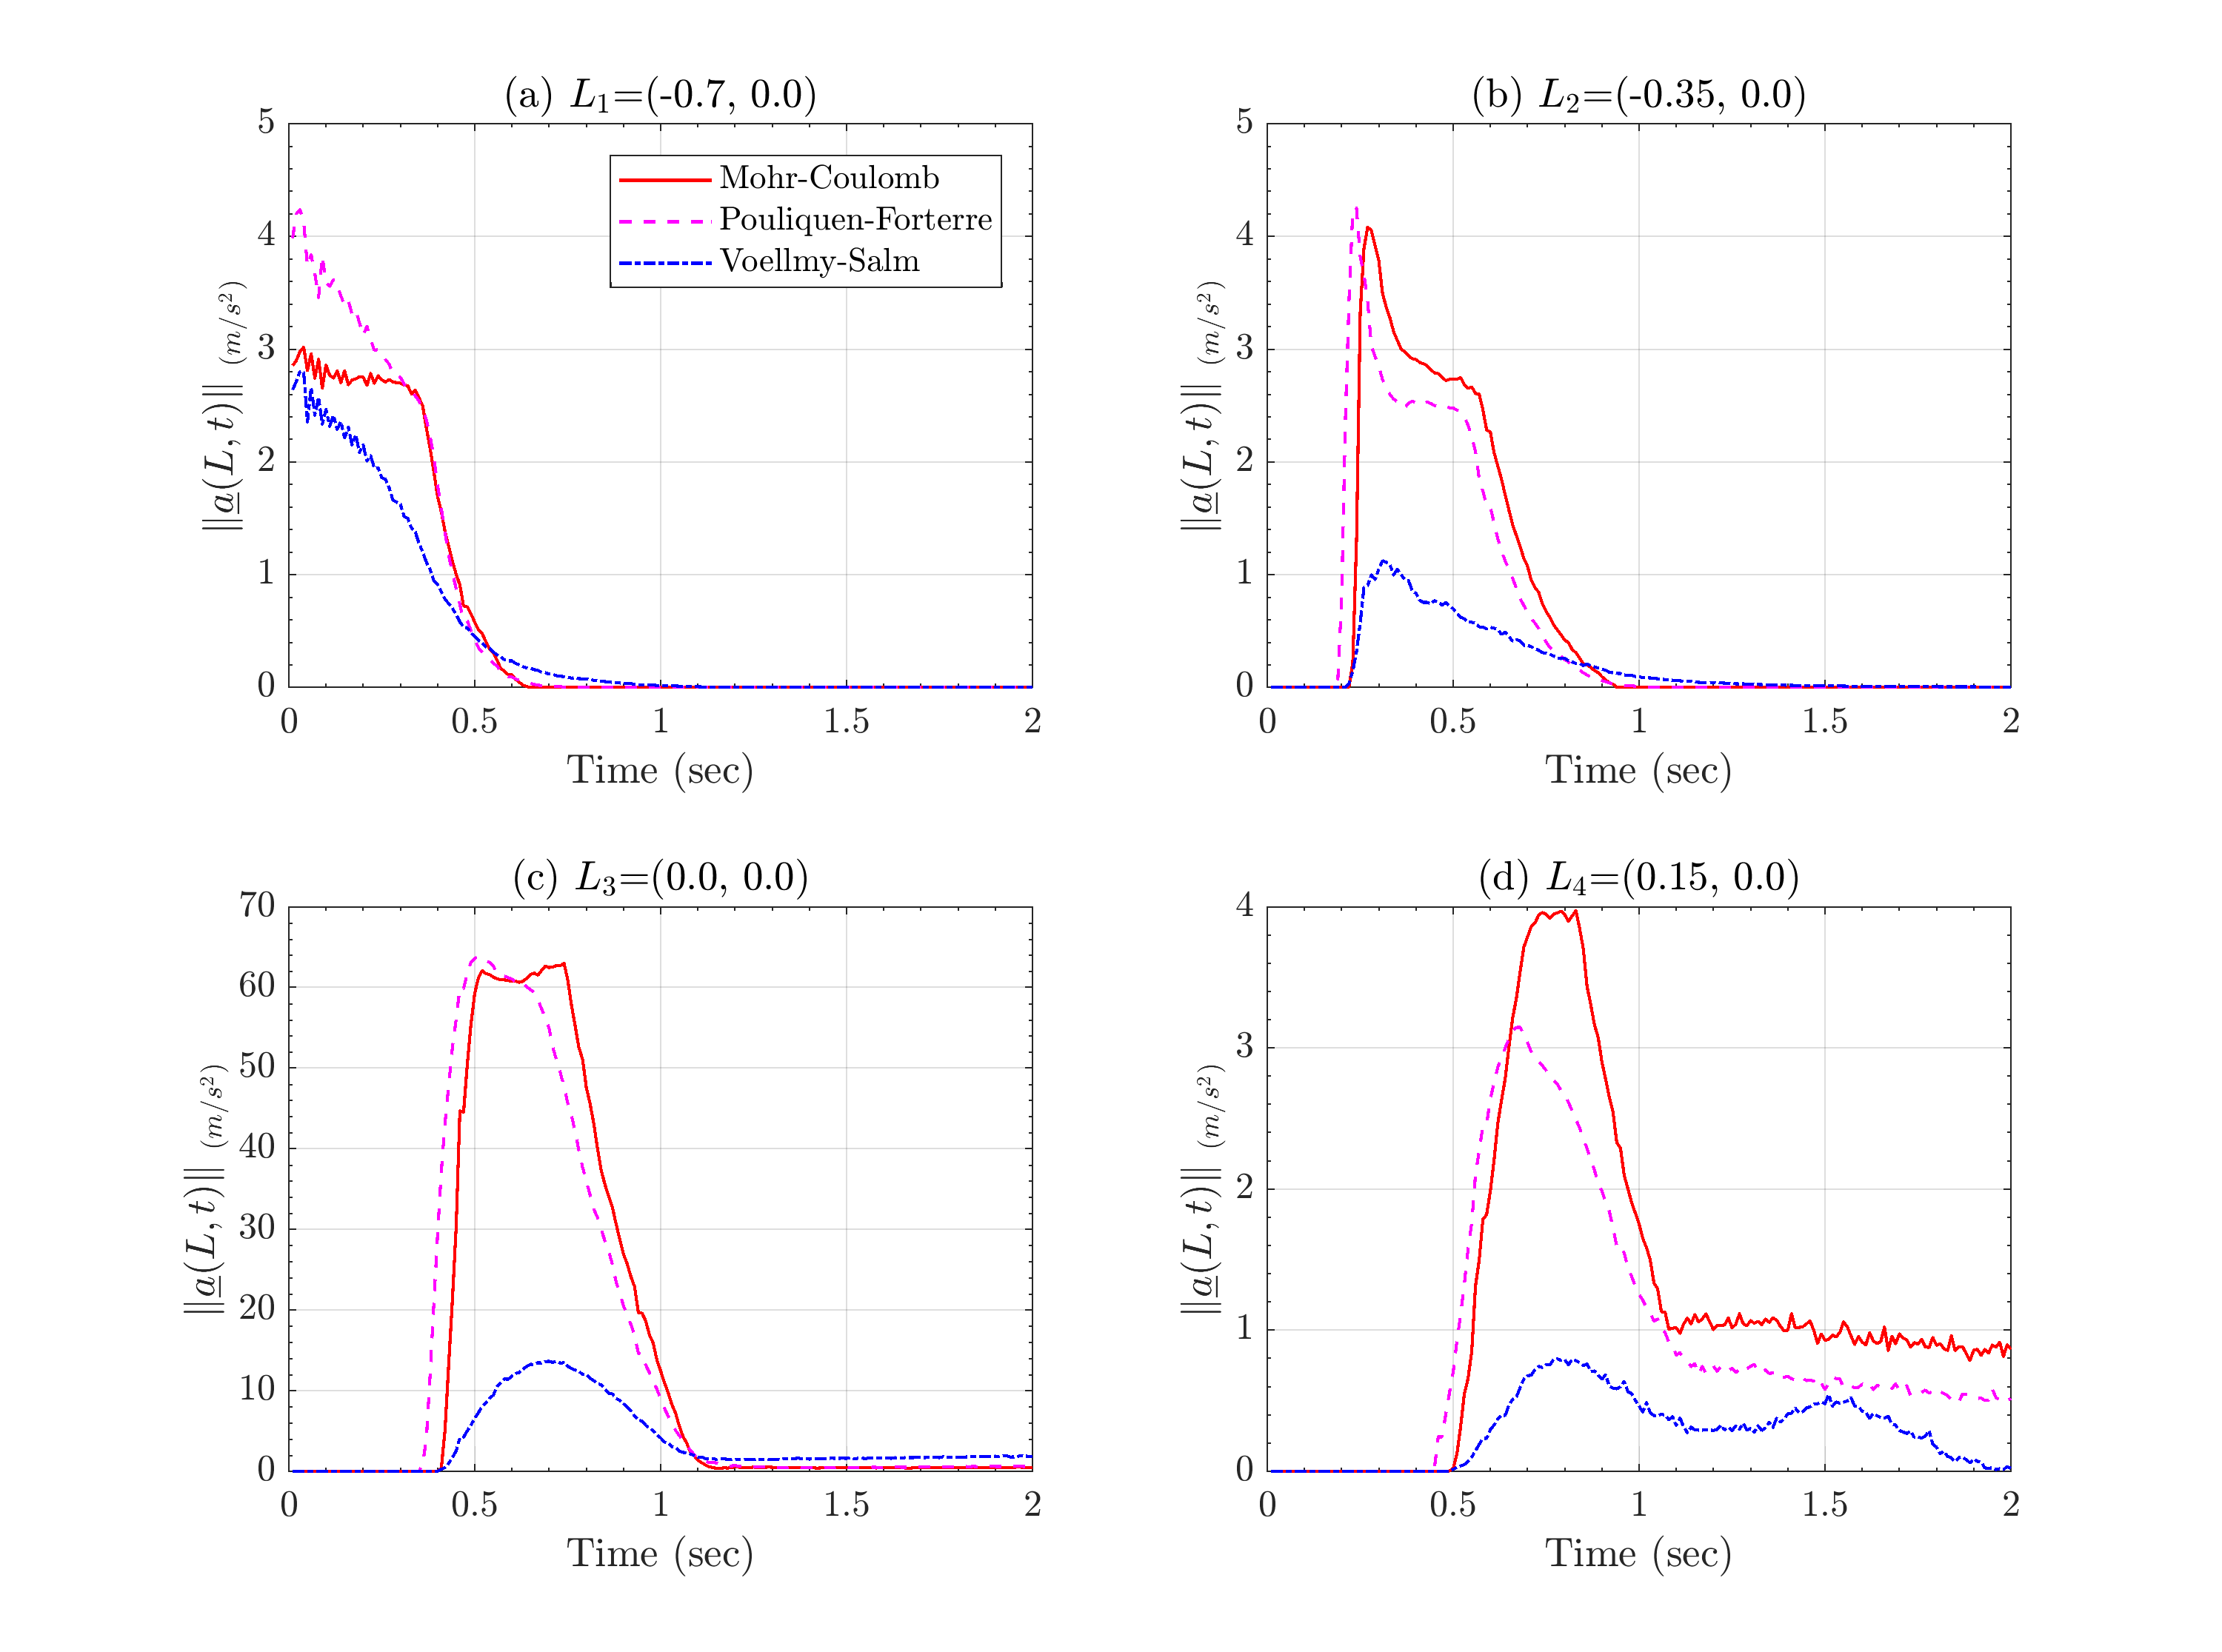
\includegraphics[width=1\textwidth]{InclinedPlane/Acceleration/accel_meanL.png}
        \caption{Comparison between mean values of flow acceleration (computed from LHS), $\Vert \underline{a} \Vert(L,t)$, recorded at locations of interest, $L_i, \ _{i=1,...,4}$.}
        \label{fig:Ramp-LM-AccL-means}
\end{figure}


\newpage
\subsubsection{Forces and Powers}

\begin{itemize}
\item	\textbf{LHS$_1$}

\begin{figure}[H]
        \centering
        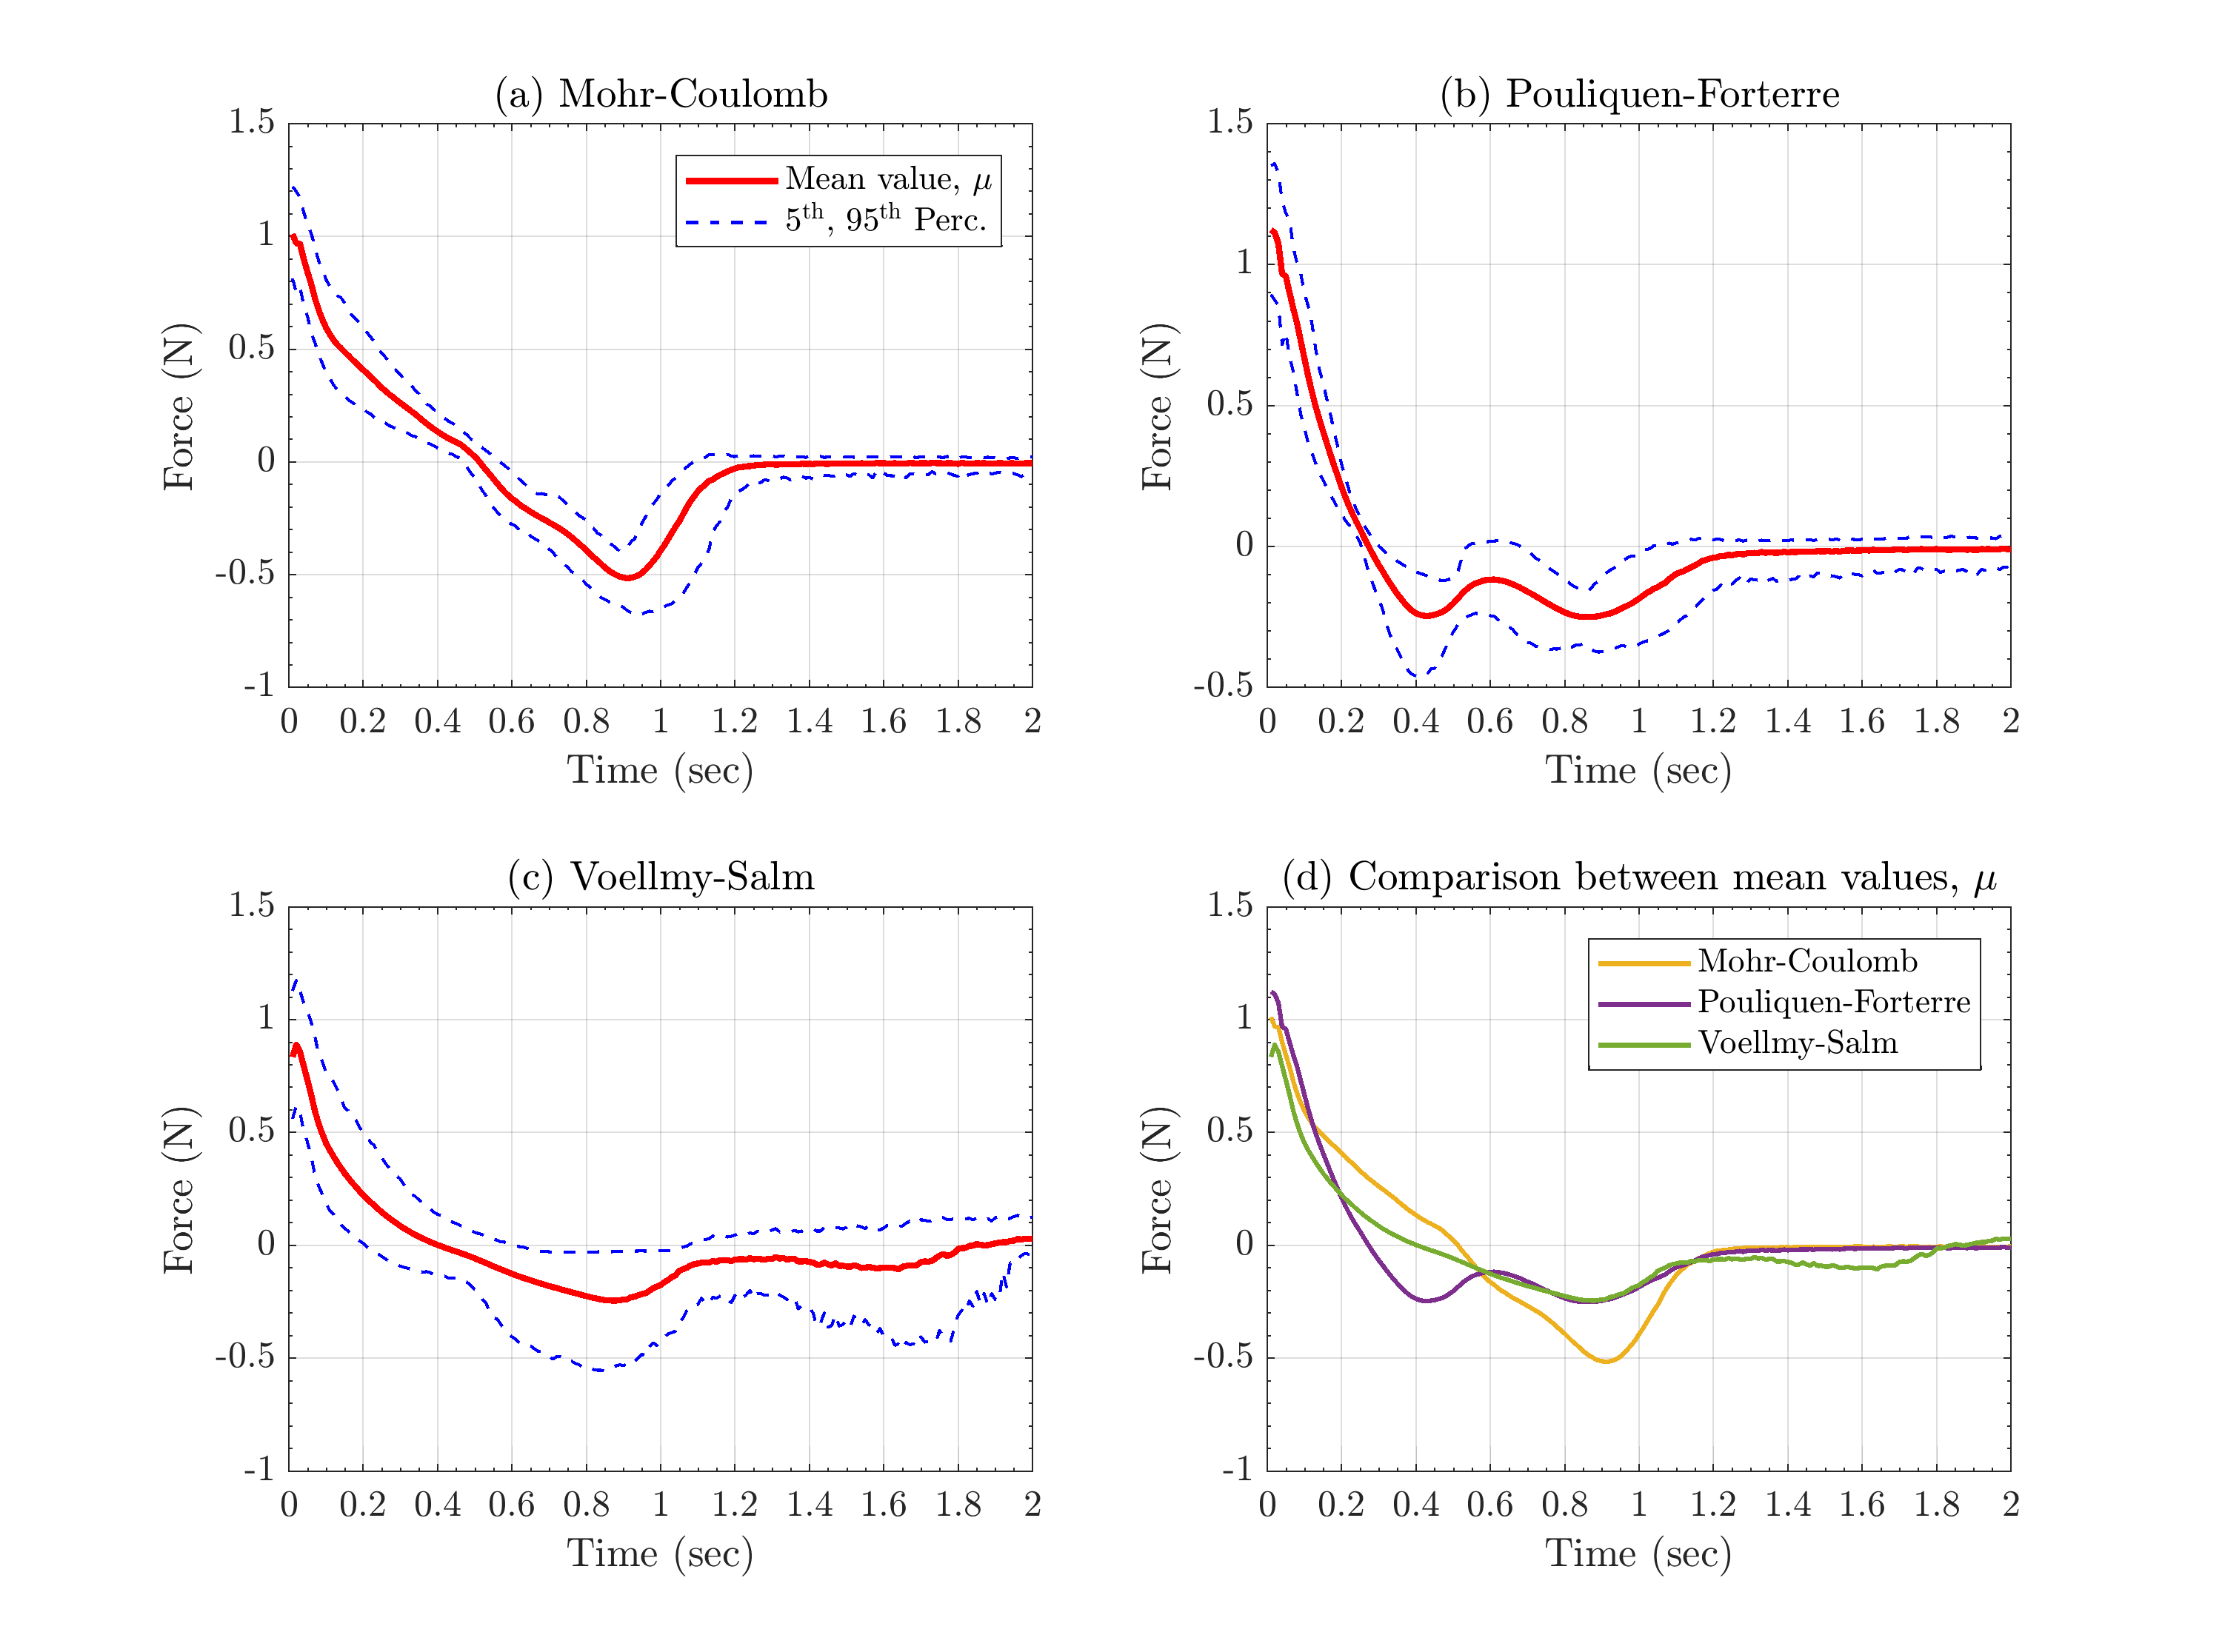
\includegraphics[width=1\textwidth]{InclinedPlane/Forces_Powers/LHS1/FLHS1x.png}
        \caption{Comparison between mean values of flow acceleration (computed from LHS), $\Vert \underline{a} \Vert(L,t)$, recorded at locations of interest, $L_i, \ _{i=1,...,4}$.}
        \label{fig:Ramp-LHS1-Fx-spatial}
\end{figure}

\begin{figure}[H]
        \centering
        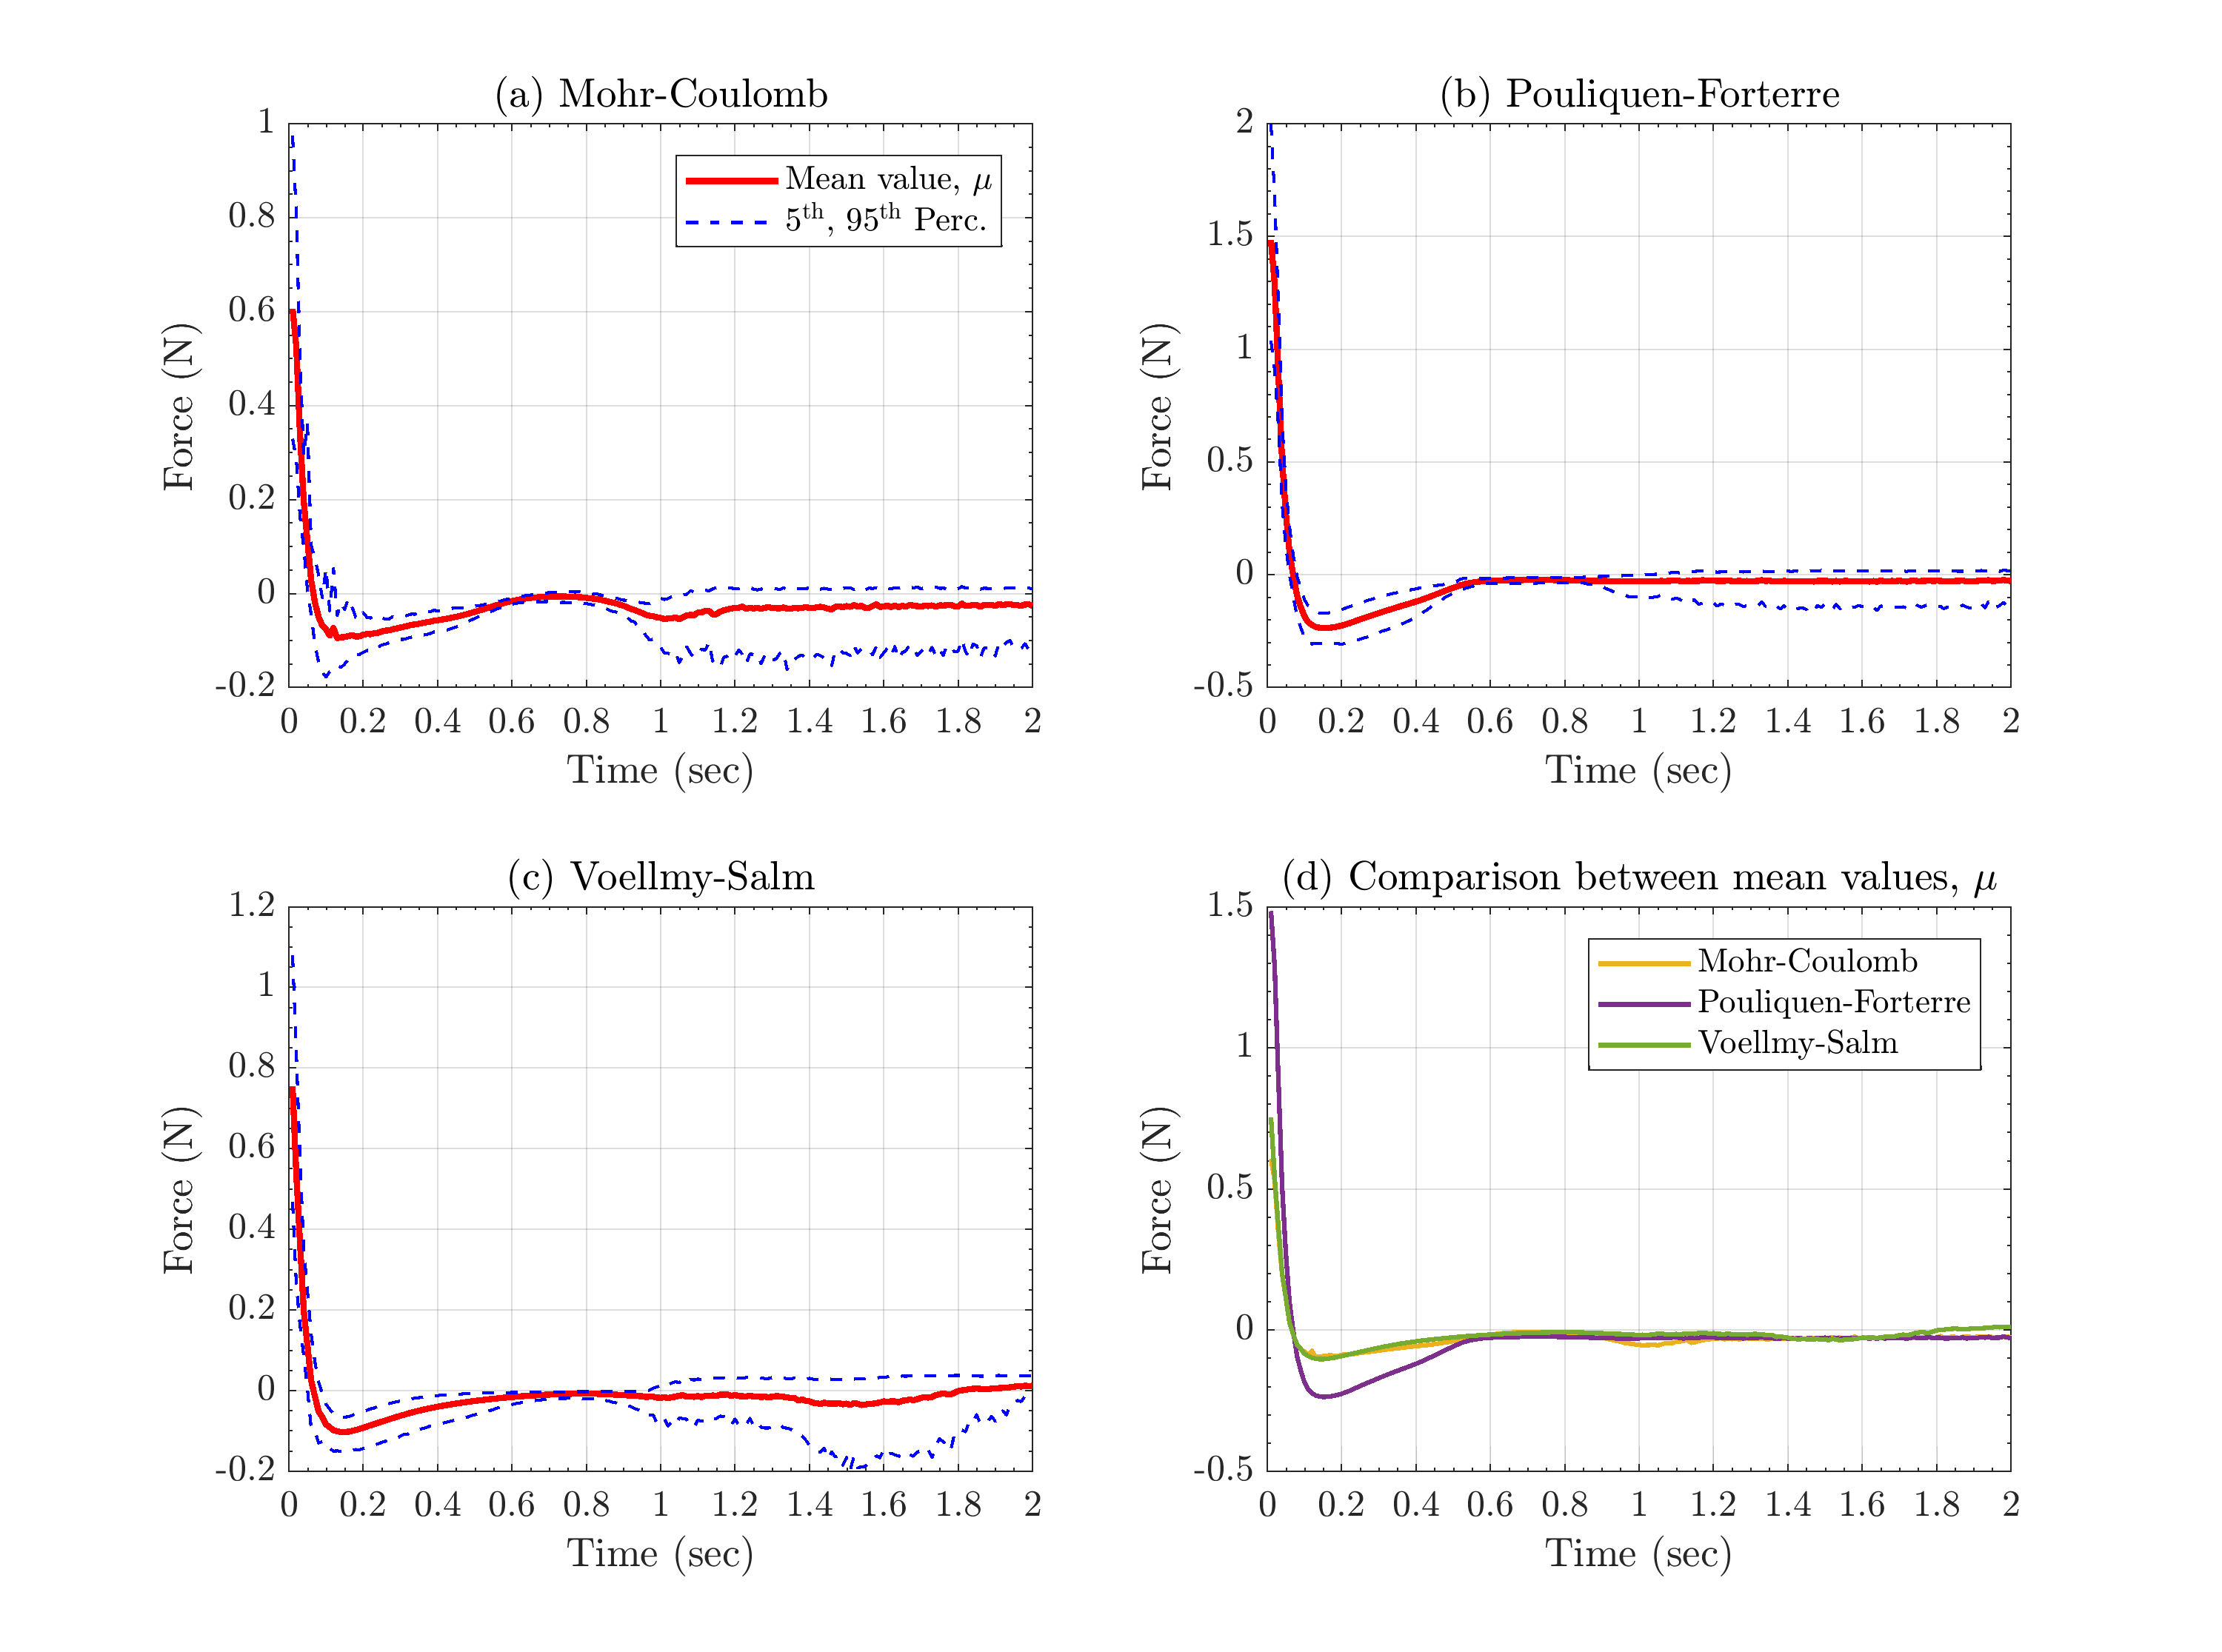
\includegraphics[width=1\textwidth]{InclinedPlane/Forces_Powers/LHS1/FLHS1y.png}
        \caption{Comparison between mean values of flow acceleration (computed from LHS), $\Vert \underline{a} \Vert(L,t)$, recorded at locations of interest, $L_i, \ _{i=1,...,4}$.}
        \label{fig:Ramp-LHS1-Fy-spatial}
\end{figure}

\begin{figure}[H]
        \centering
        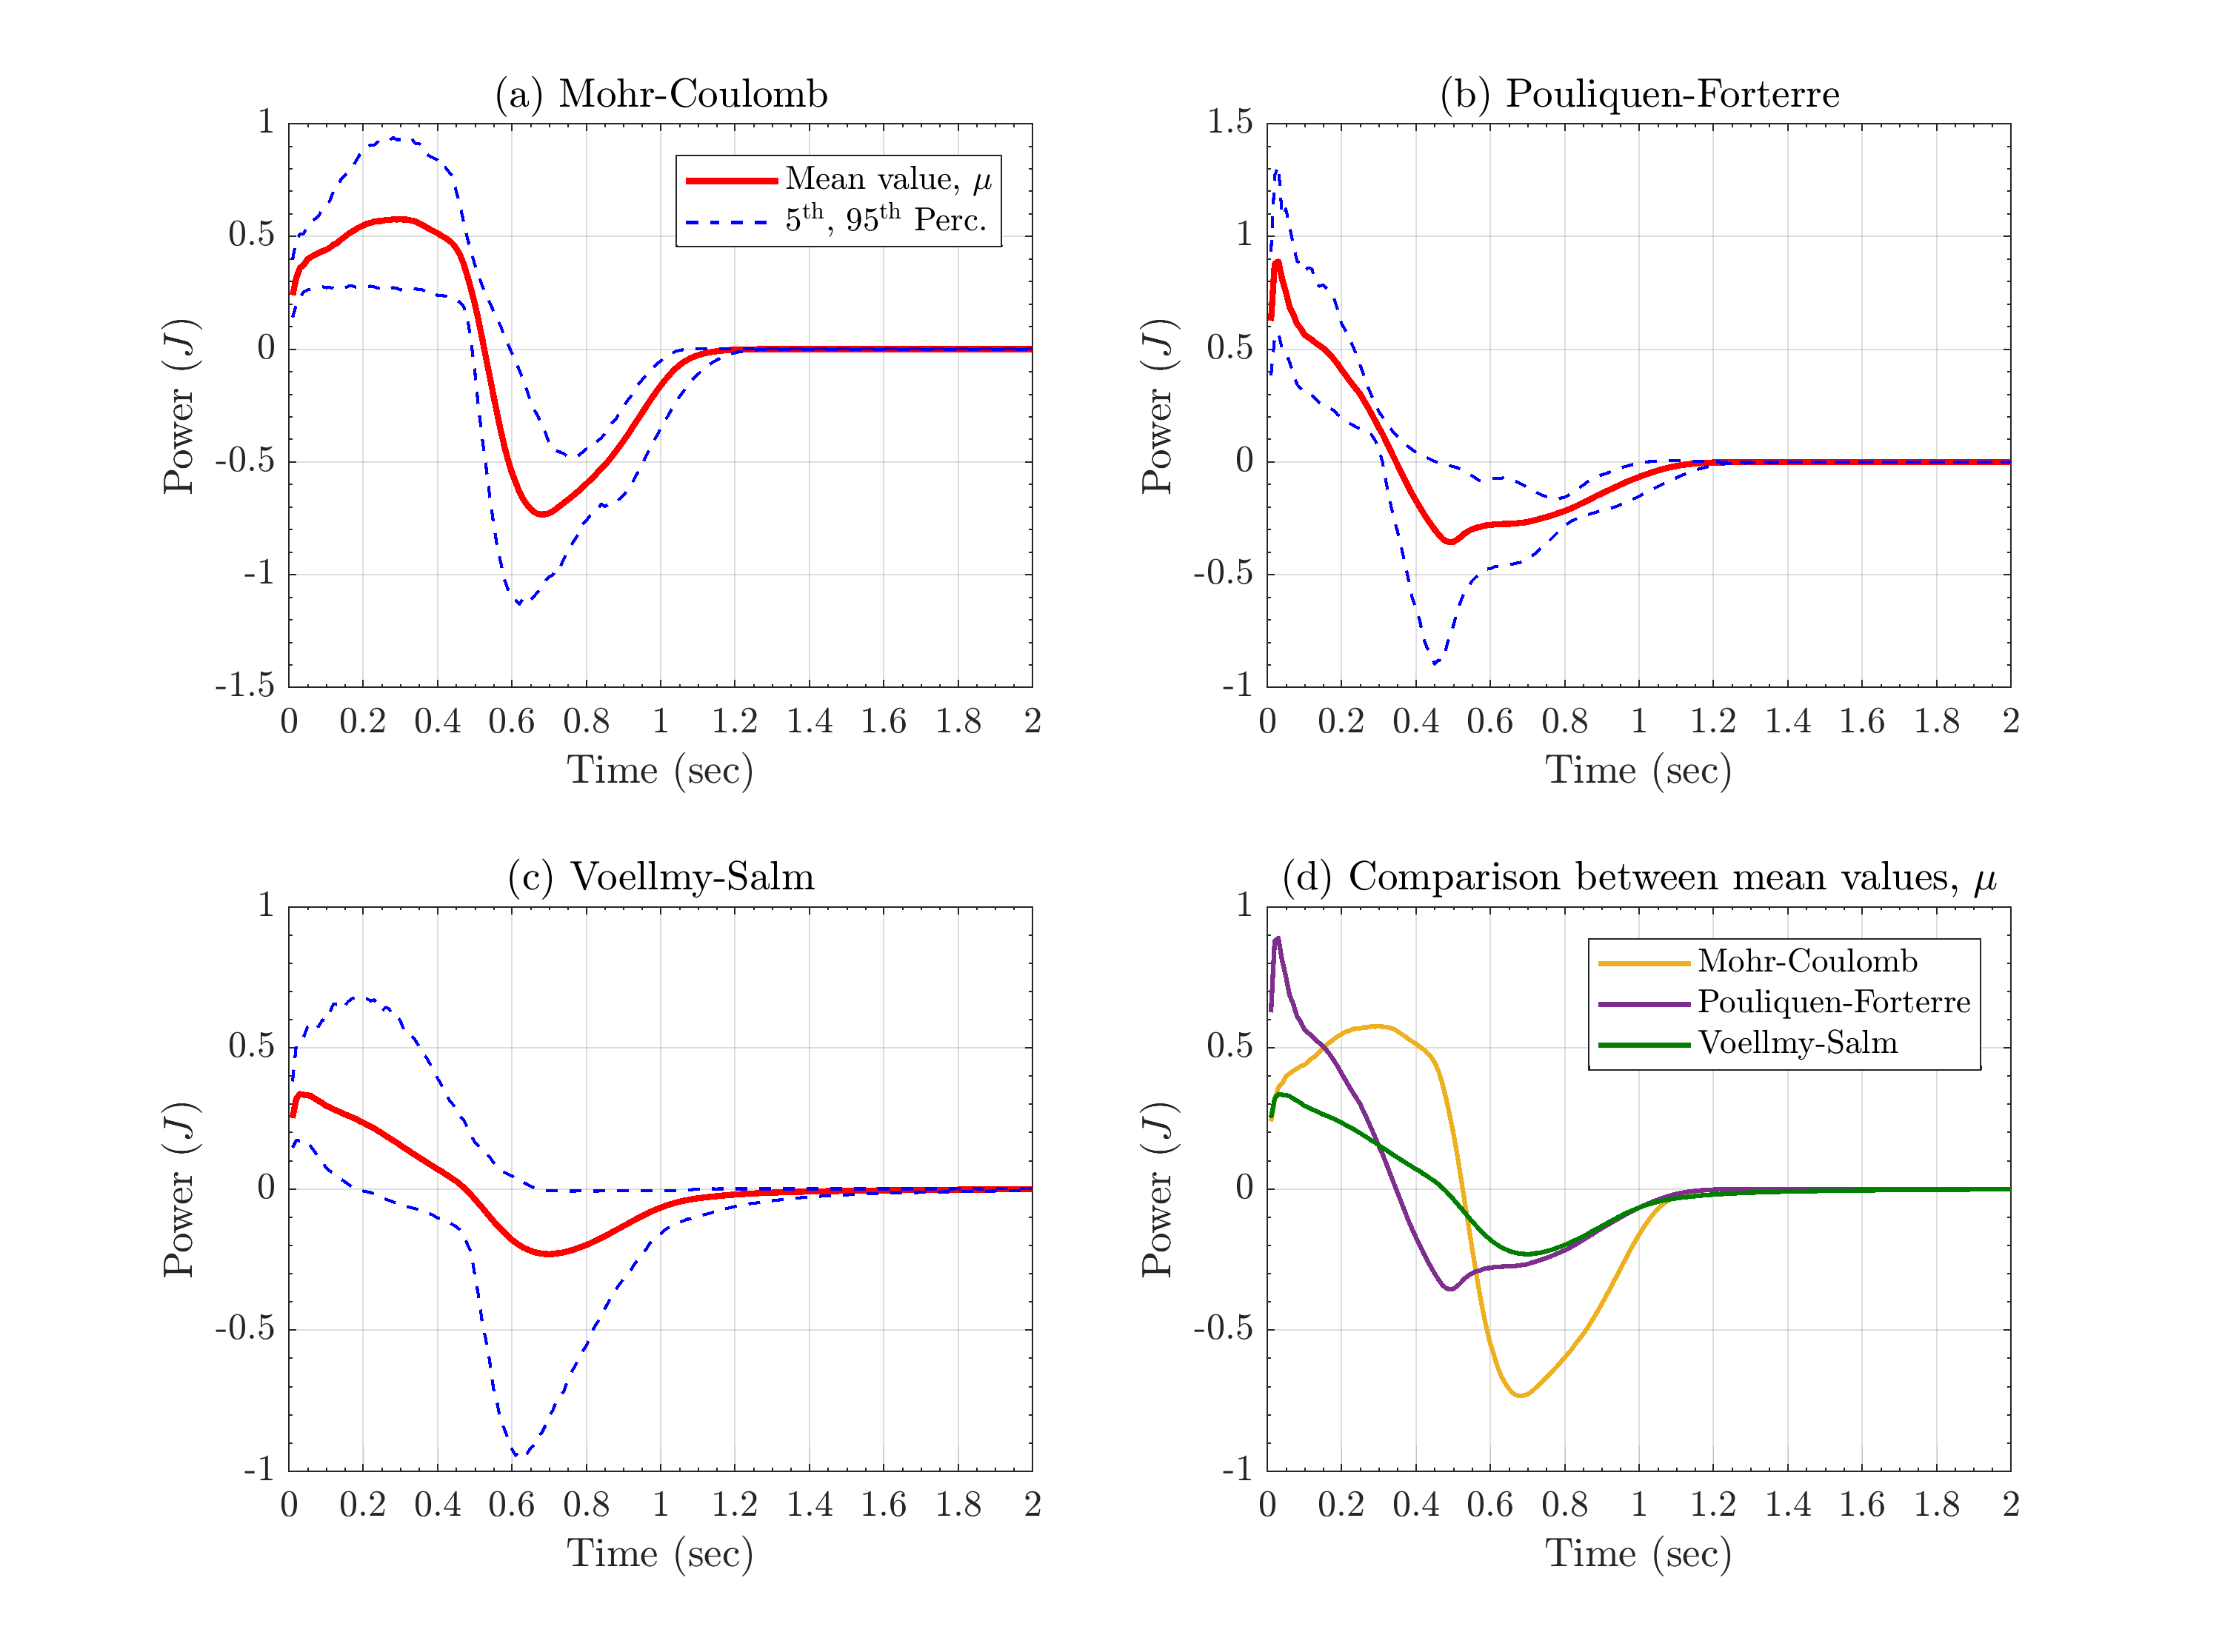
\includegraphics[width=1\textwidth]{InclinedPlane/Forces_Powers/LHS1/PLHS1.png}
        \caption{Comparison between mean values of flow acceleration (computed from LHS), $\Vert \underline{a} \Vert(L,t)$, recorded at locations of interest, $L_i, \ _{i=1,...,4}$.}
        \label{fig:Ramp-LHS1-Power-spatial}
\end{figure}

\newpage
\item	\textbf{LHS$_2$}

\begin{figure}[H]
        \centering
        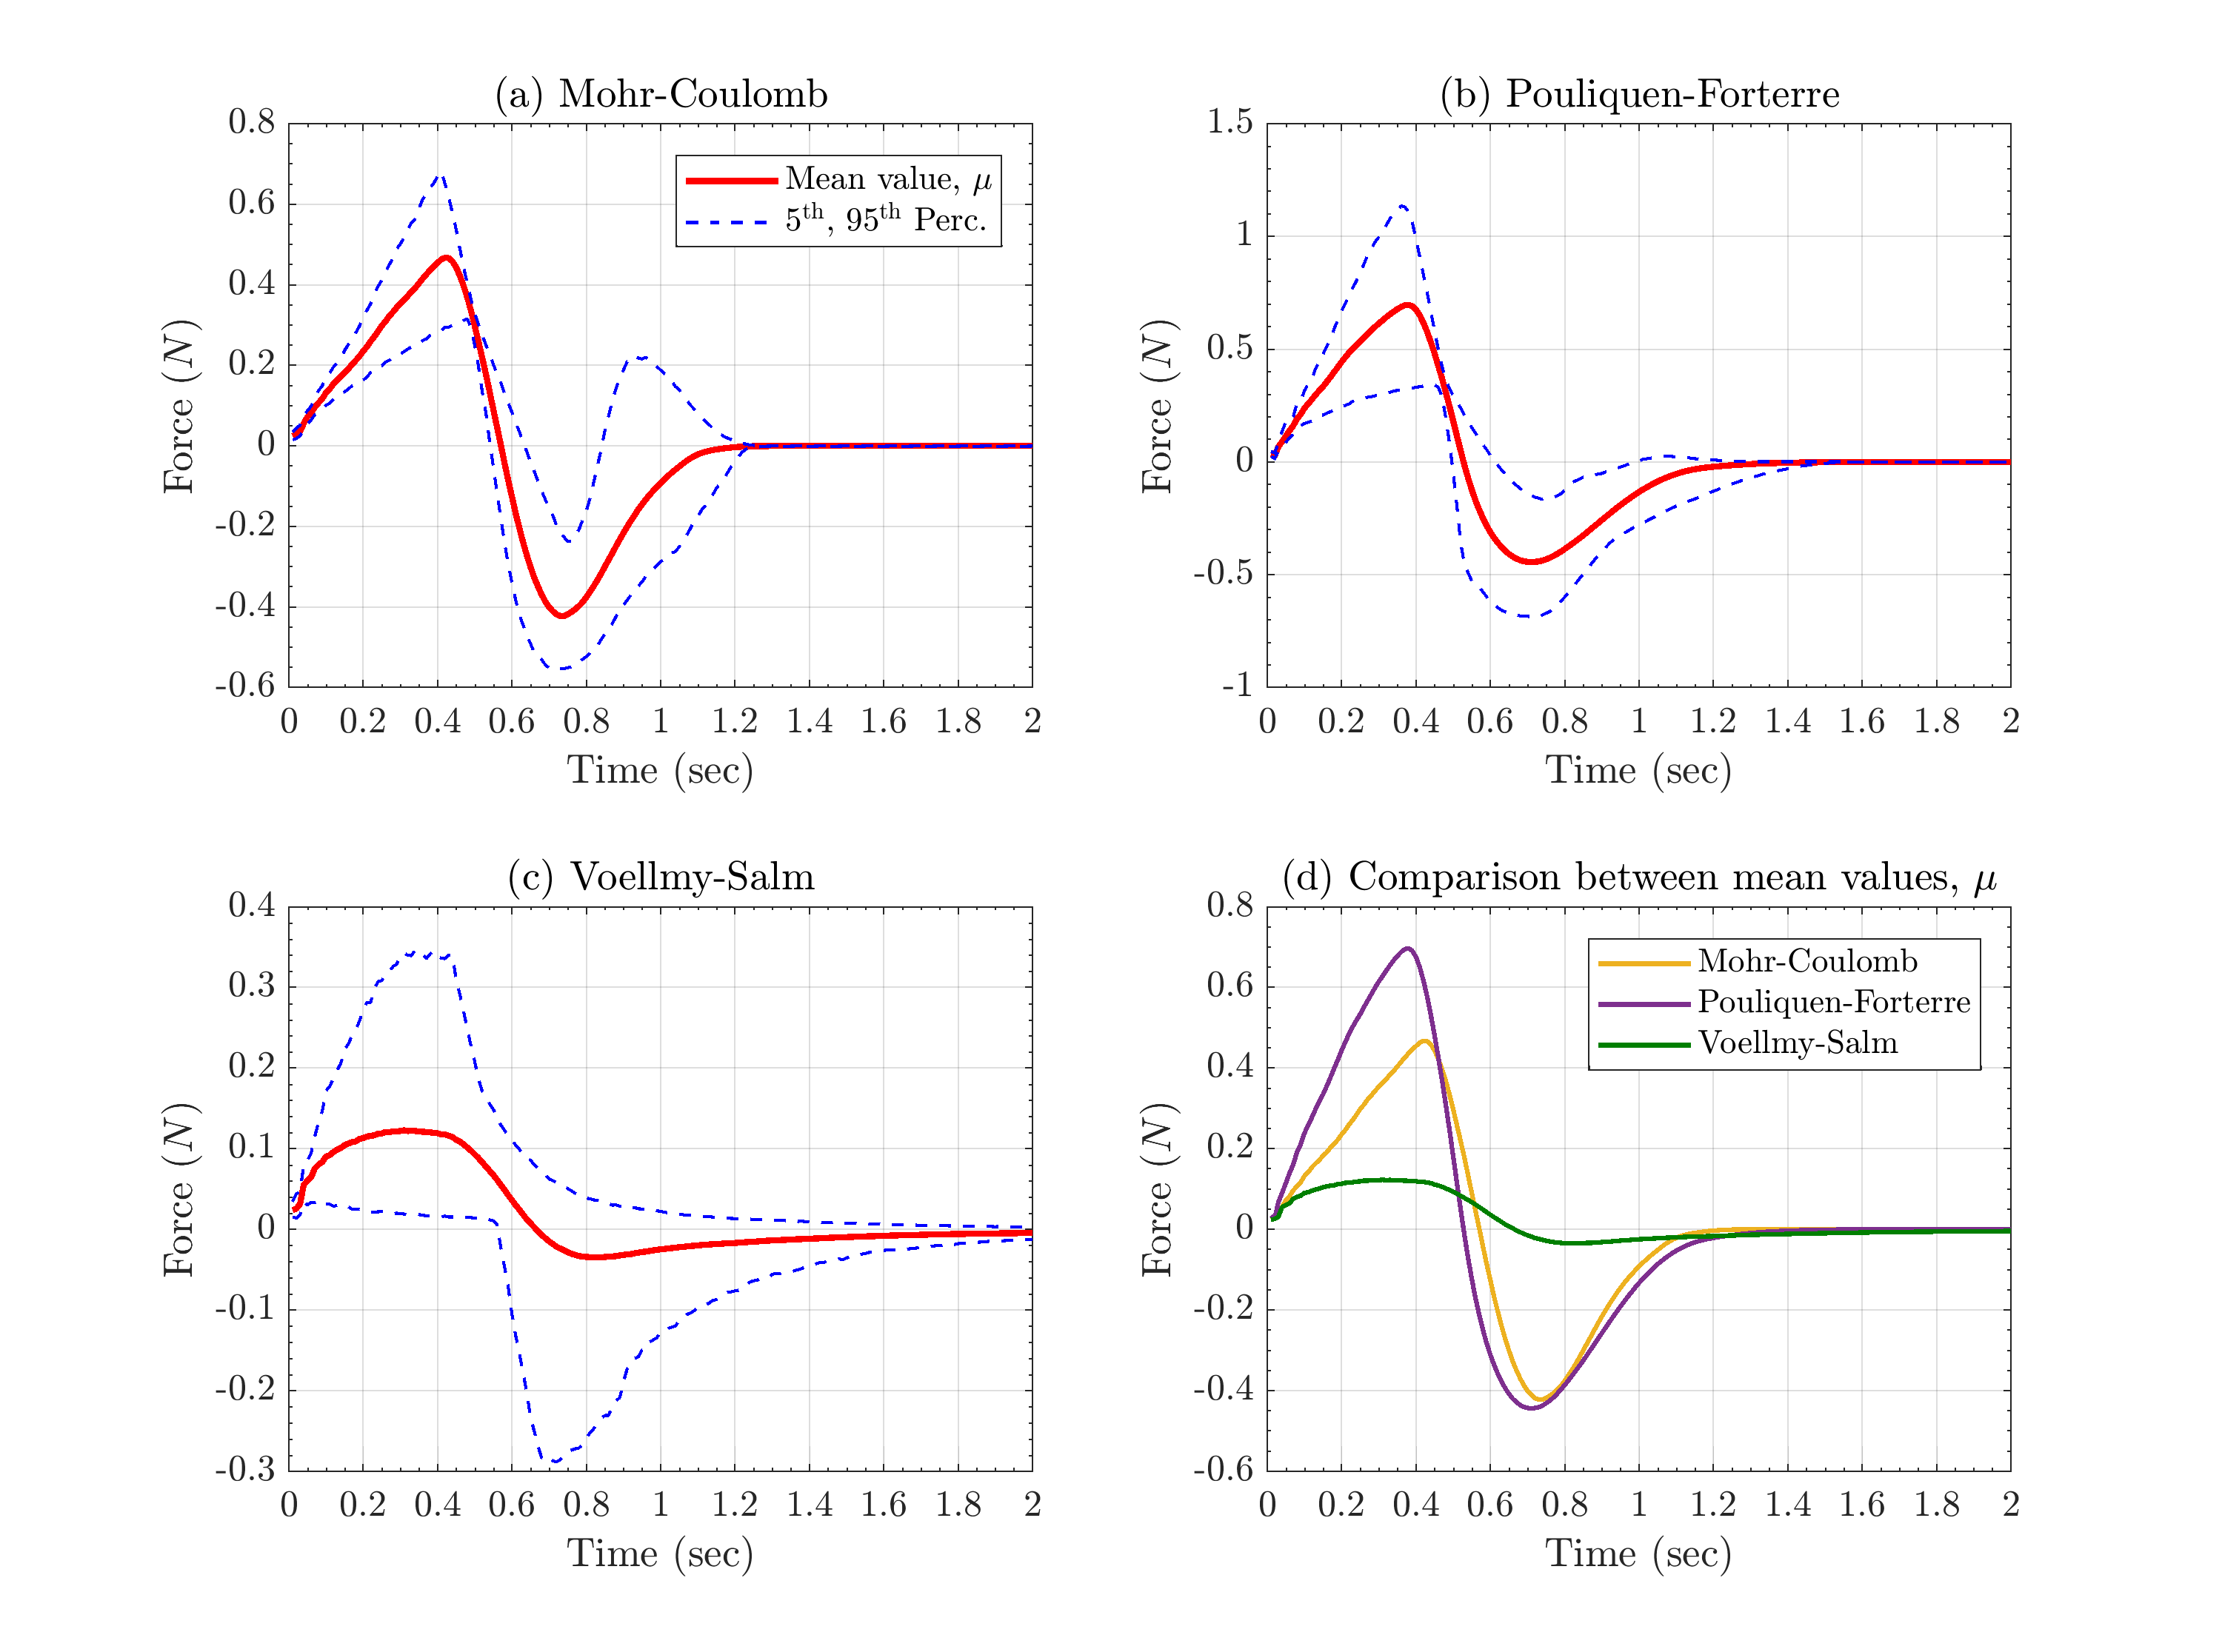
\includegraphics[width=1\textwidth]{InclinedPlane/Forces_Powers/LHS2/FLHS2x.png}
        \caption{Comparison between mean values of flow acceleration (computed from LHS), $\Vert \underline{a} \Vert(L,t)$, recorded at locations of interest, $L_i, \ _{i=1,...,4}$.}
        \label{fig:Ramp-LHS2-Fx-spatial}
\end{figure}

\begin{figure}[H]
        \centering
        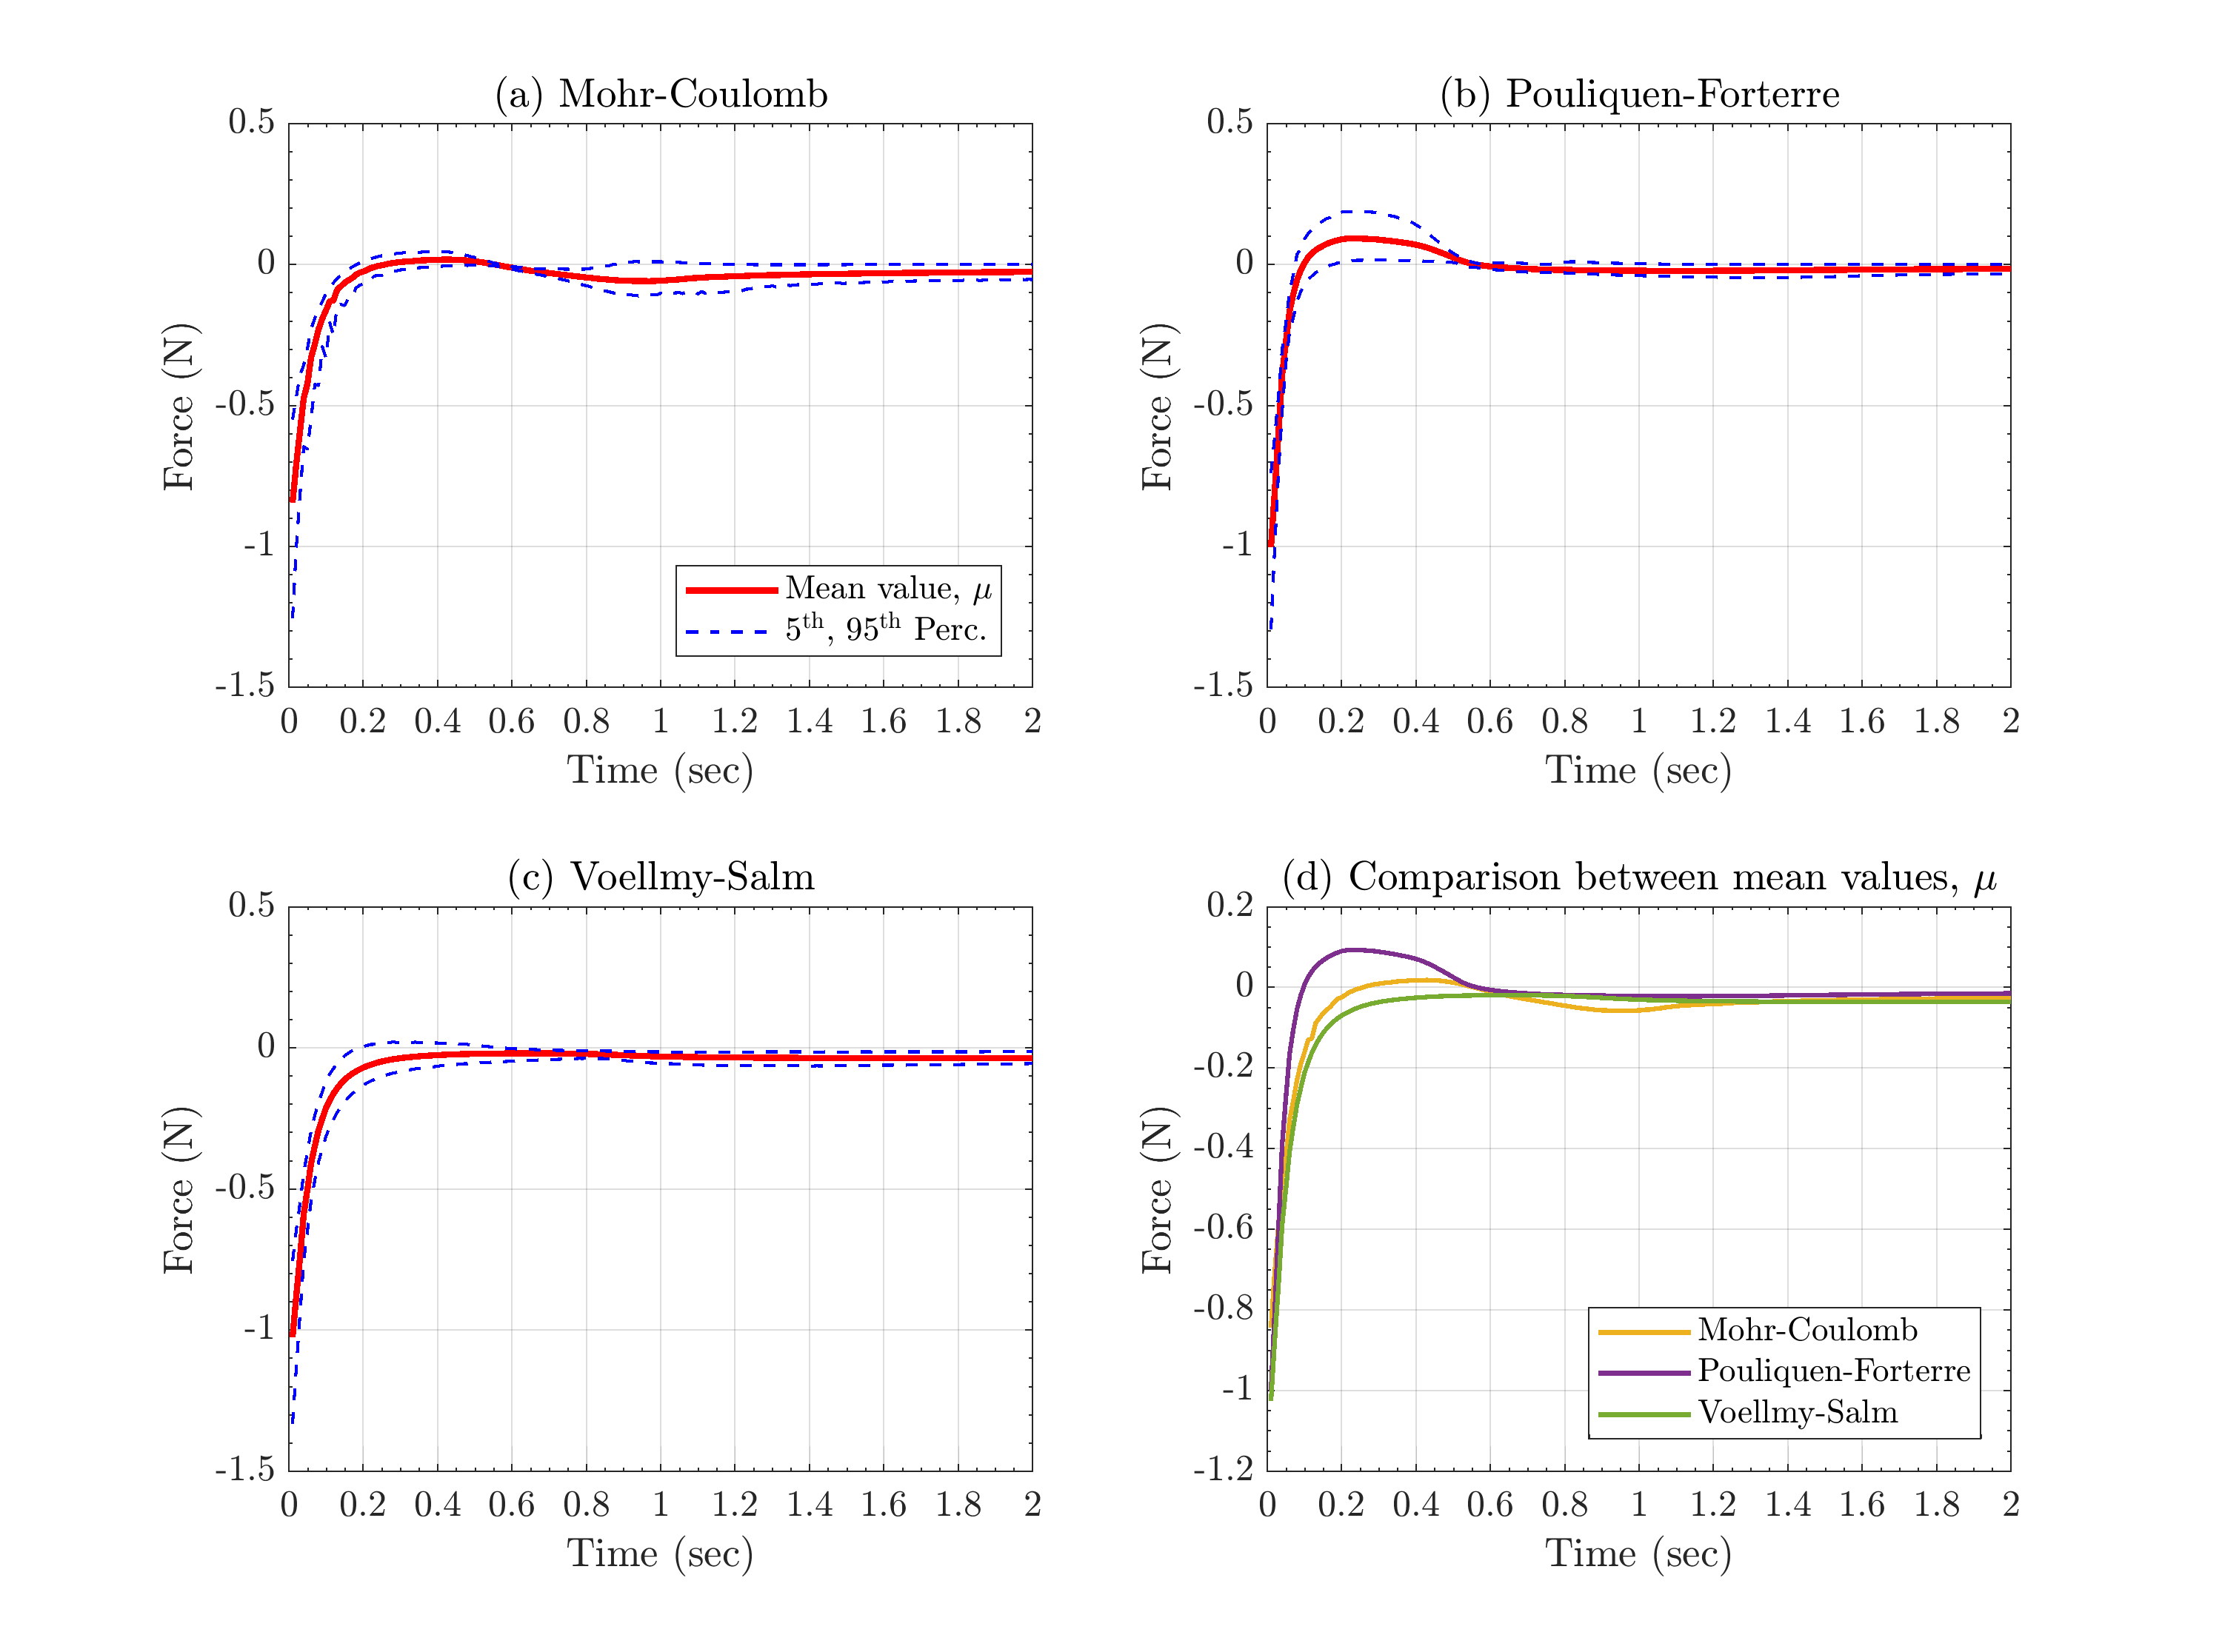
\includegraphics[width=1\textwidth]{InclinedPlane/Forces_Powers/LHS2/FLHS2y.png}
        \caption{Comparison between mean values of flow acceleration (computed from LHS), $\Vert \underline{a} \Vert(L,t)$, recorded at locations of interest, $L_i, \ _{i=1,...,4}$.}
        \label{fig:Ramp-LHS2-Fy-spatial}
\end{figure}

\begin{figure}[H]
        \centering
        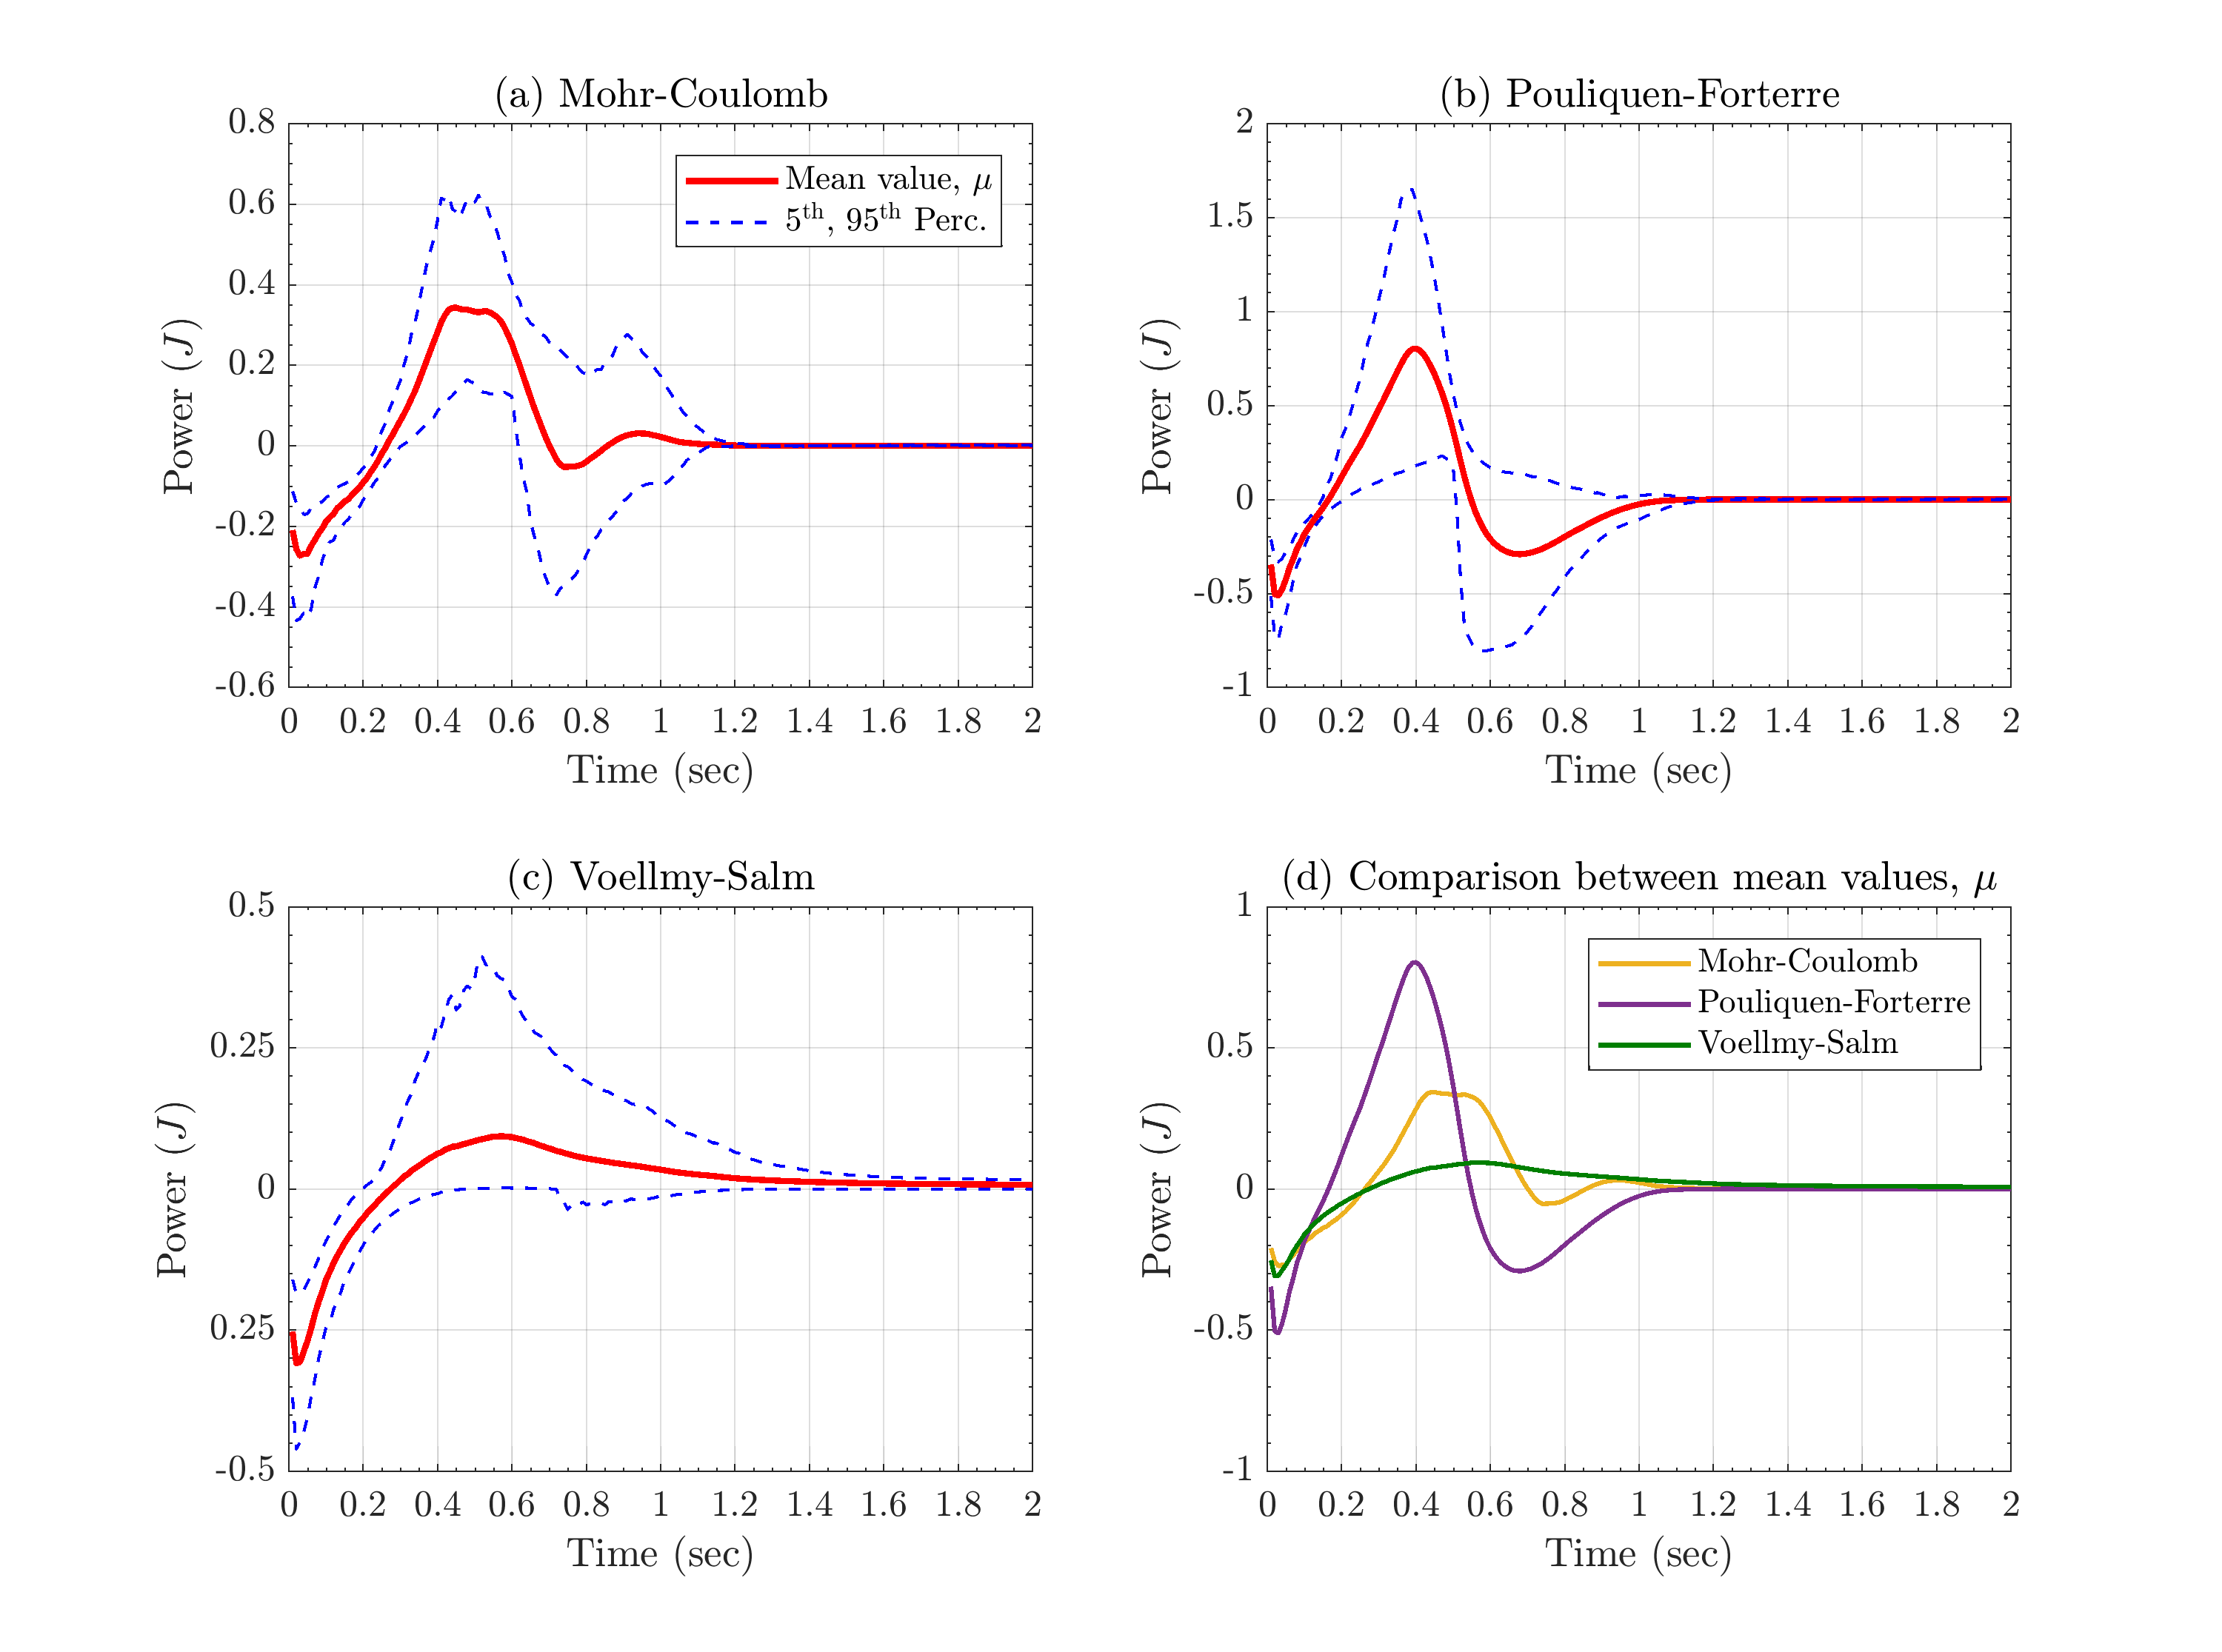
\includegraphics[width=1\textwidth]{InclinedPlane/Forces_Powers/LHS2/PLHS2.png}
        \caption{Comparison between mean values of flow acceleration (computed from LHS), $\Vert \underline{a} \Vert(L,t)$, recorded at locations of interest, $L_i, \ _{i=1,...,4}$.}
        \label{fig:Ramp-LHS2-Power-spatial}
\end{figure}

\newpage
\item	\textbf{RHS$_1$}

\begin{figure}[H]
        \centering
        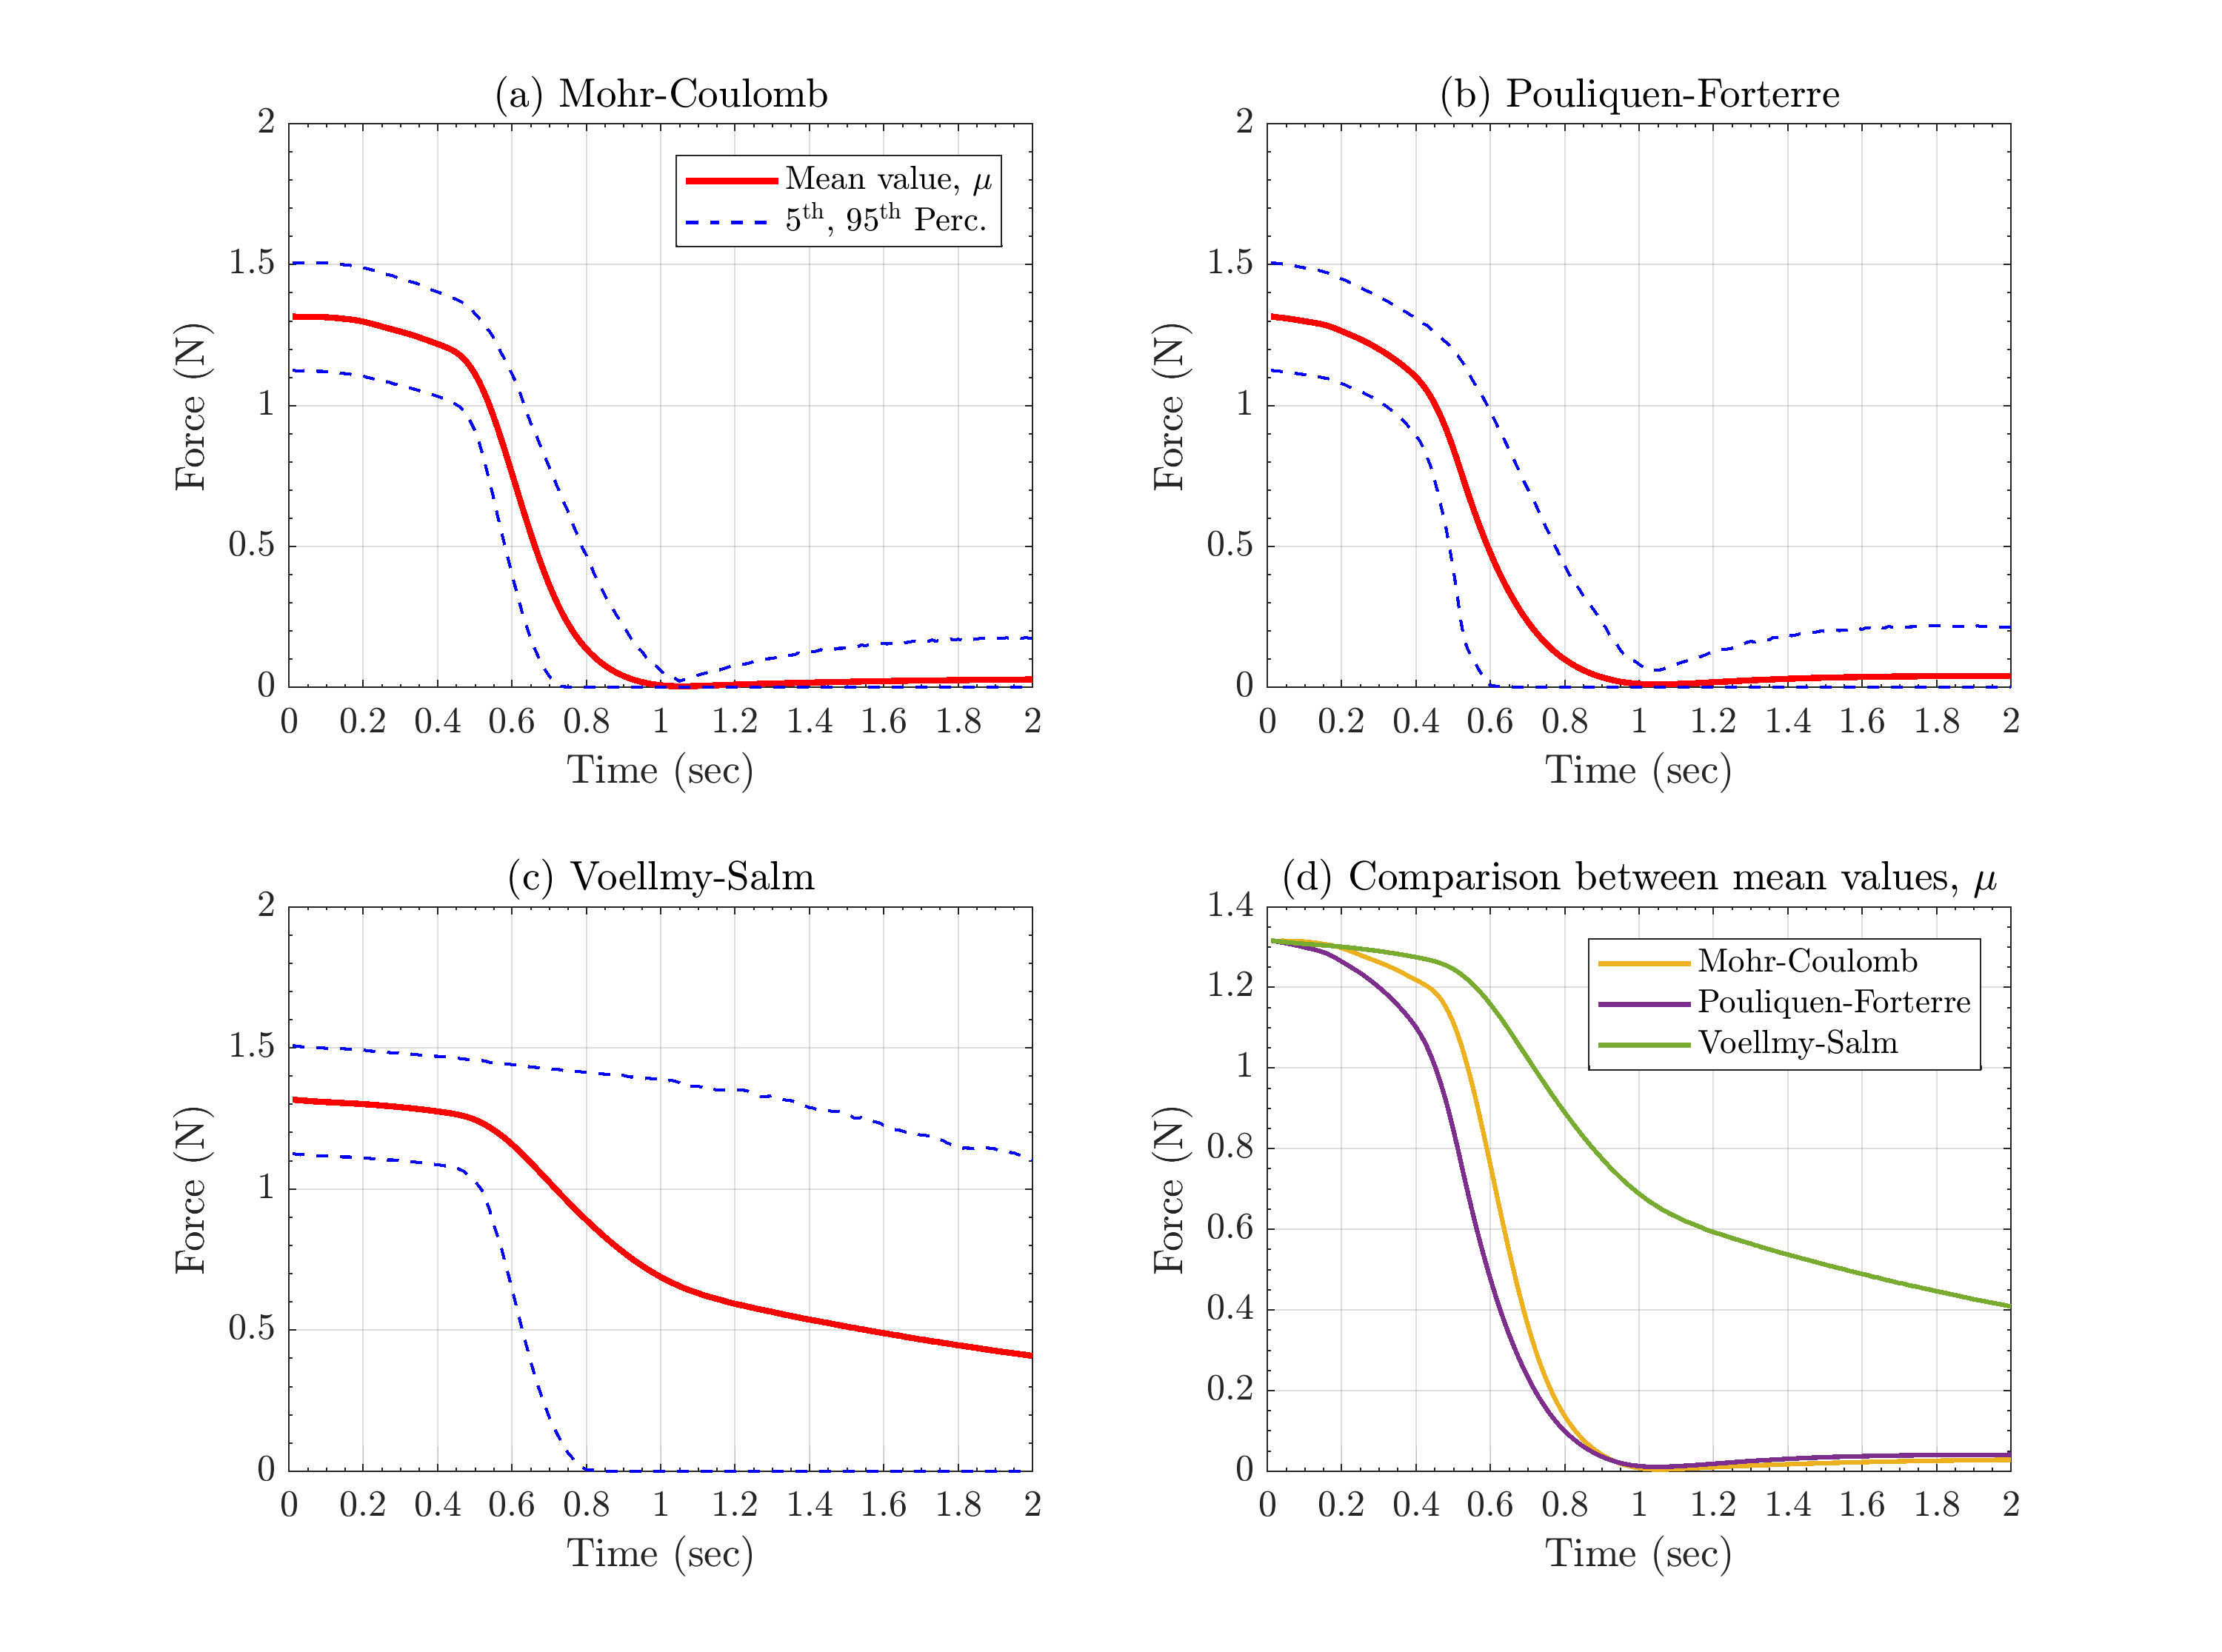
\includegraphics[width=1\textwidth]{InclinedPlane/Forces_Powers/RHS1/FRHS1x.png}
        \caption{Comparison between mean values of flow acceleration (computed from LHS), $\Vert \underline{a} \Vert(L,t)$, recorded at locations of interest, $L_i, \ _{i=1,...,4}$.}
        \label{fig:Ramp-RHS1-Fx-spatial}
\end{figure}

\begin{figure}[H]
        \centering
        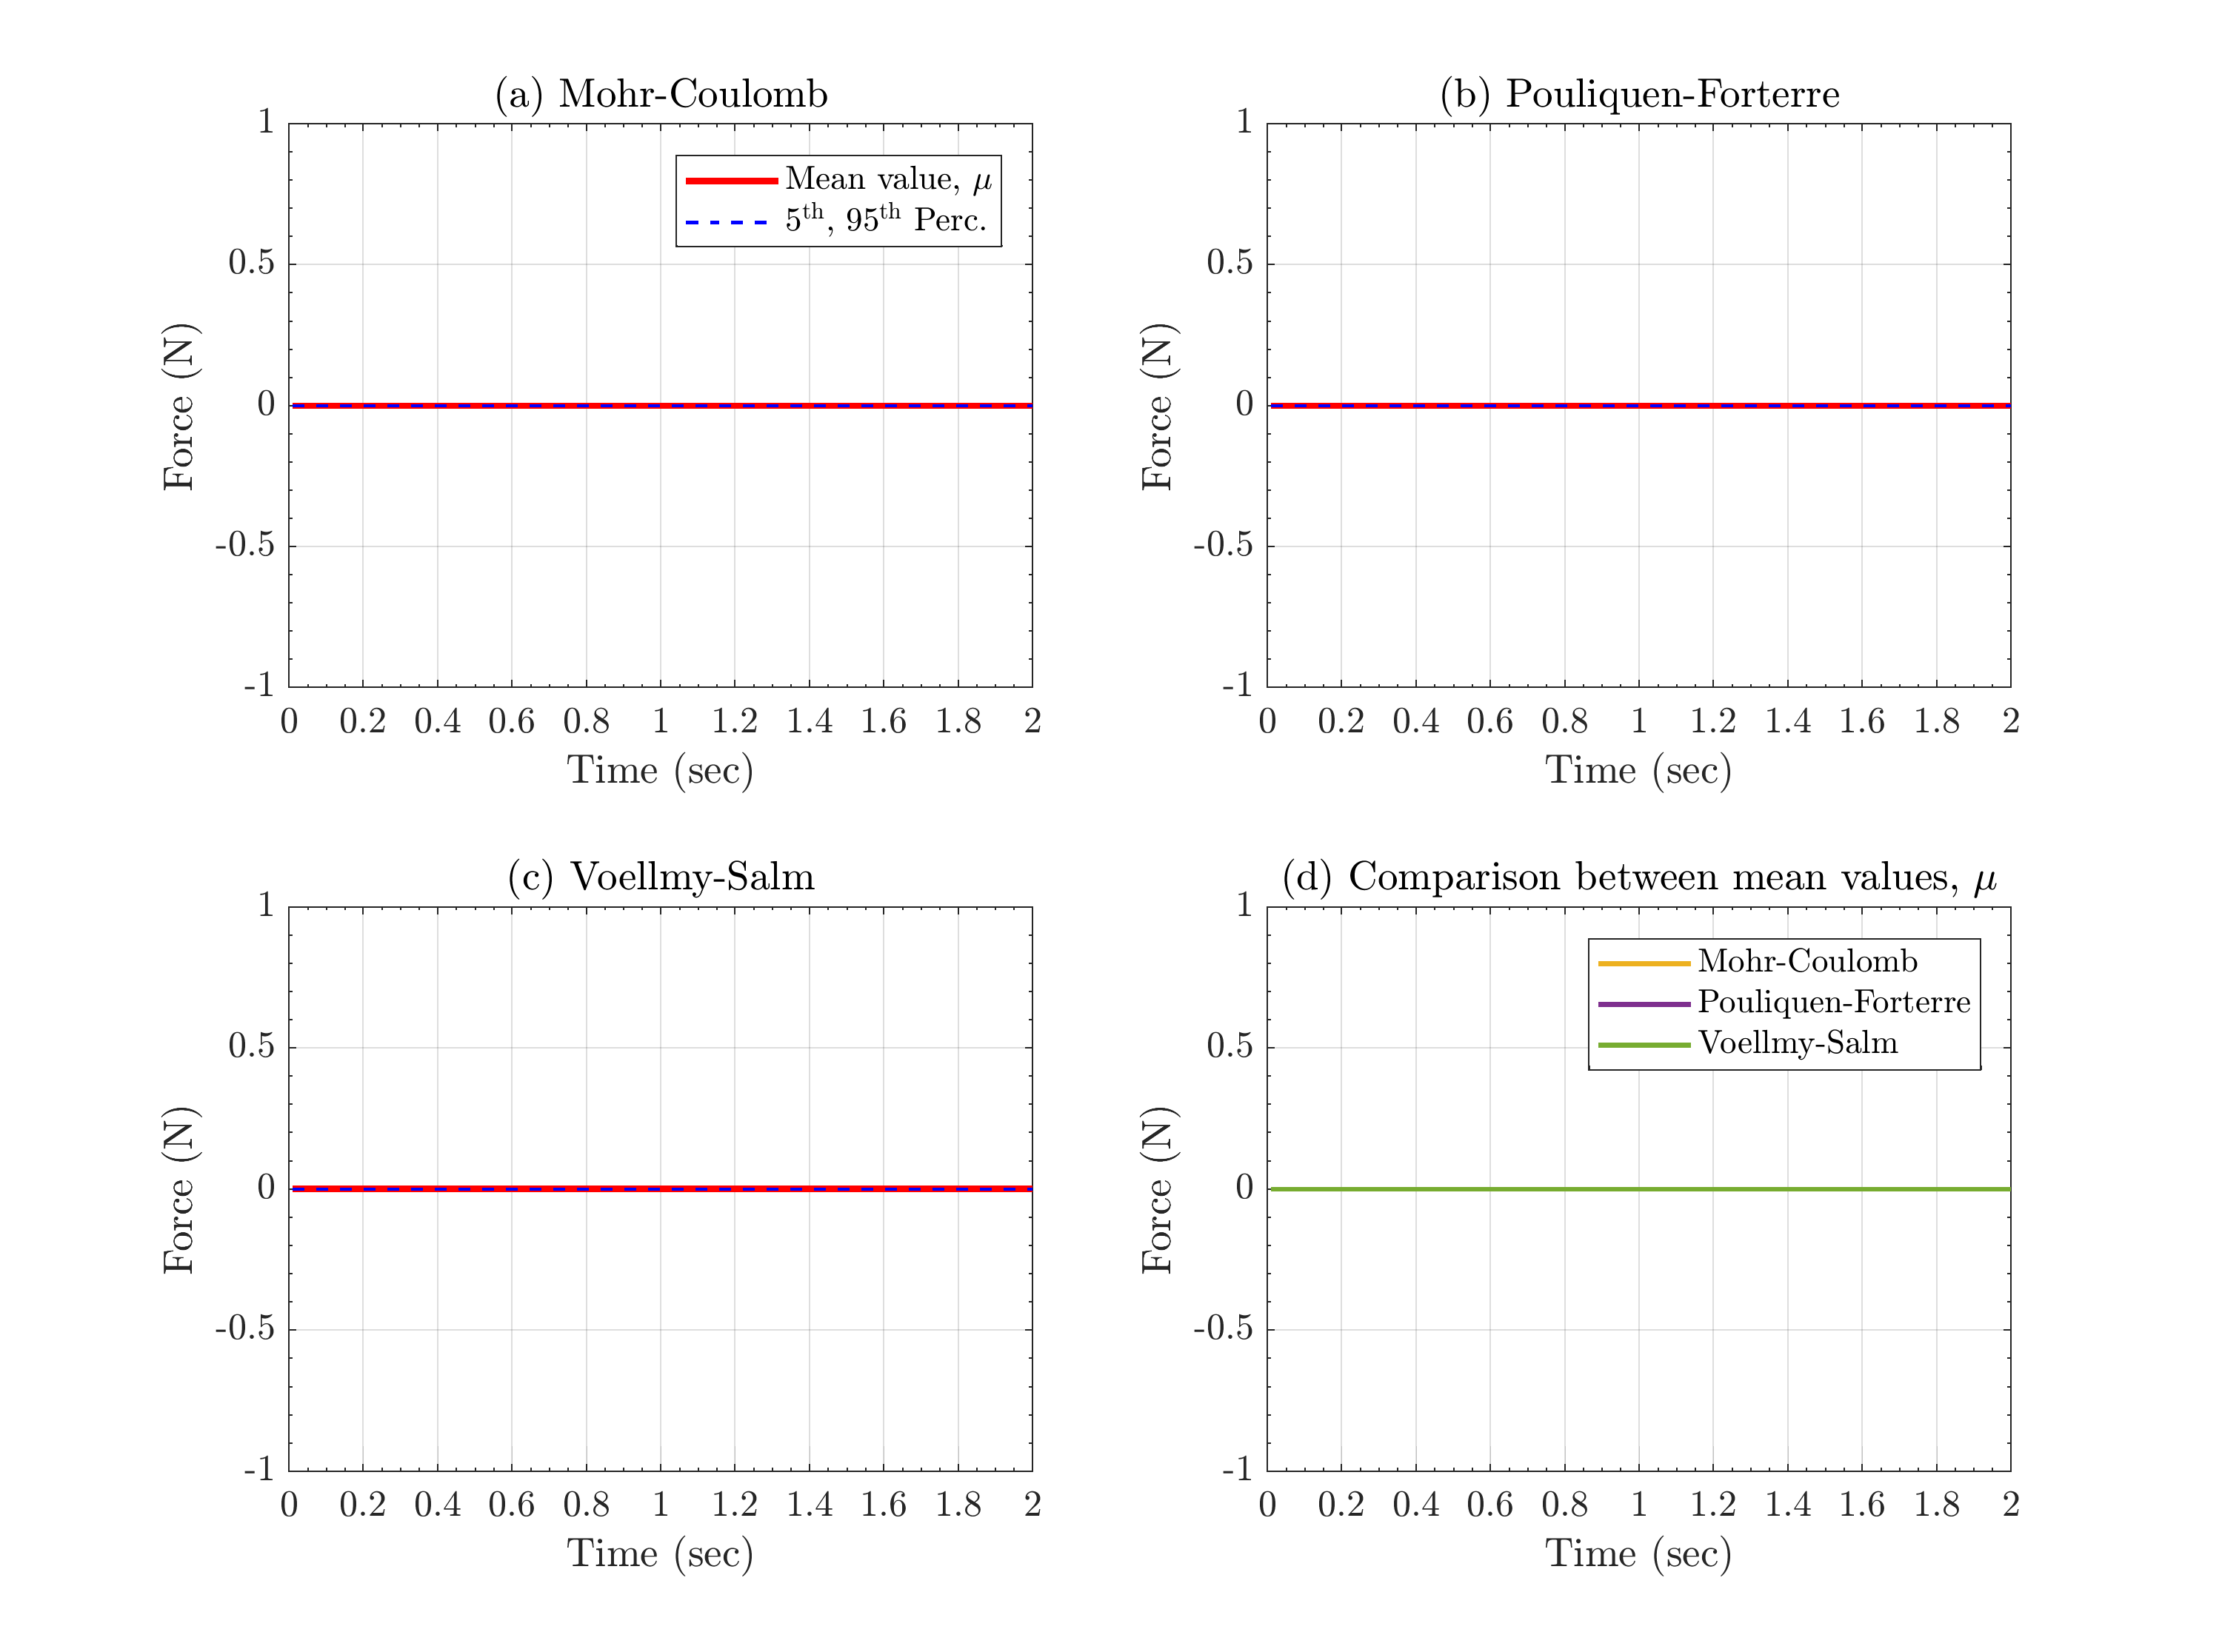
\includegraphics[width=1\textwidth]{InclinedPlane/Forces_Powers/RHS1/FRHS1y.png}
        \caption{Comparison between mean values of flow acceleration (computed from LHS), $\Vert \underline{a} \Vert(L,t)$, recorded at locations of interest, $L_i, \ _{i=1,...,4}$.}
        \label{fig:Ramp-RHS1-Fy-spatial}
\end{figure}

\begin{figure}[H]
        \centering
        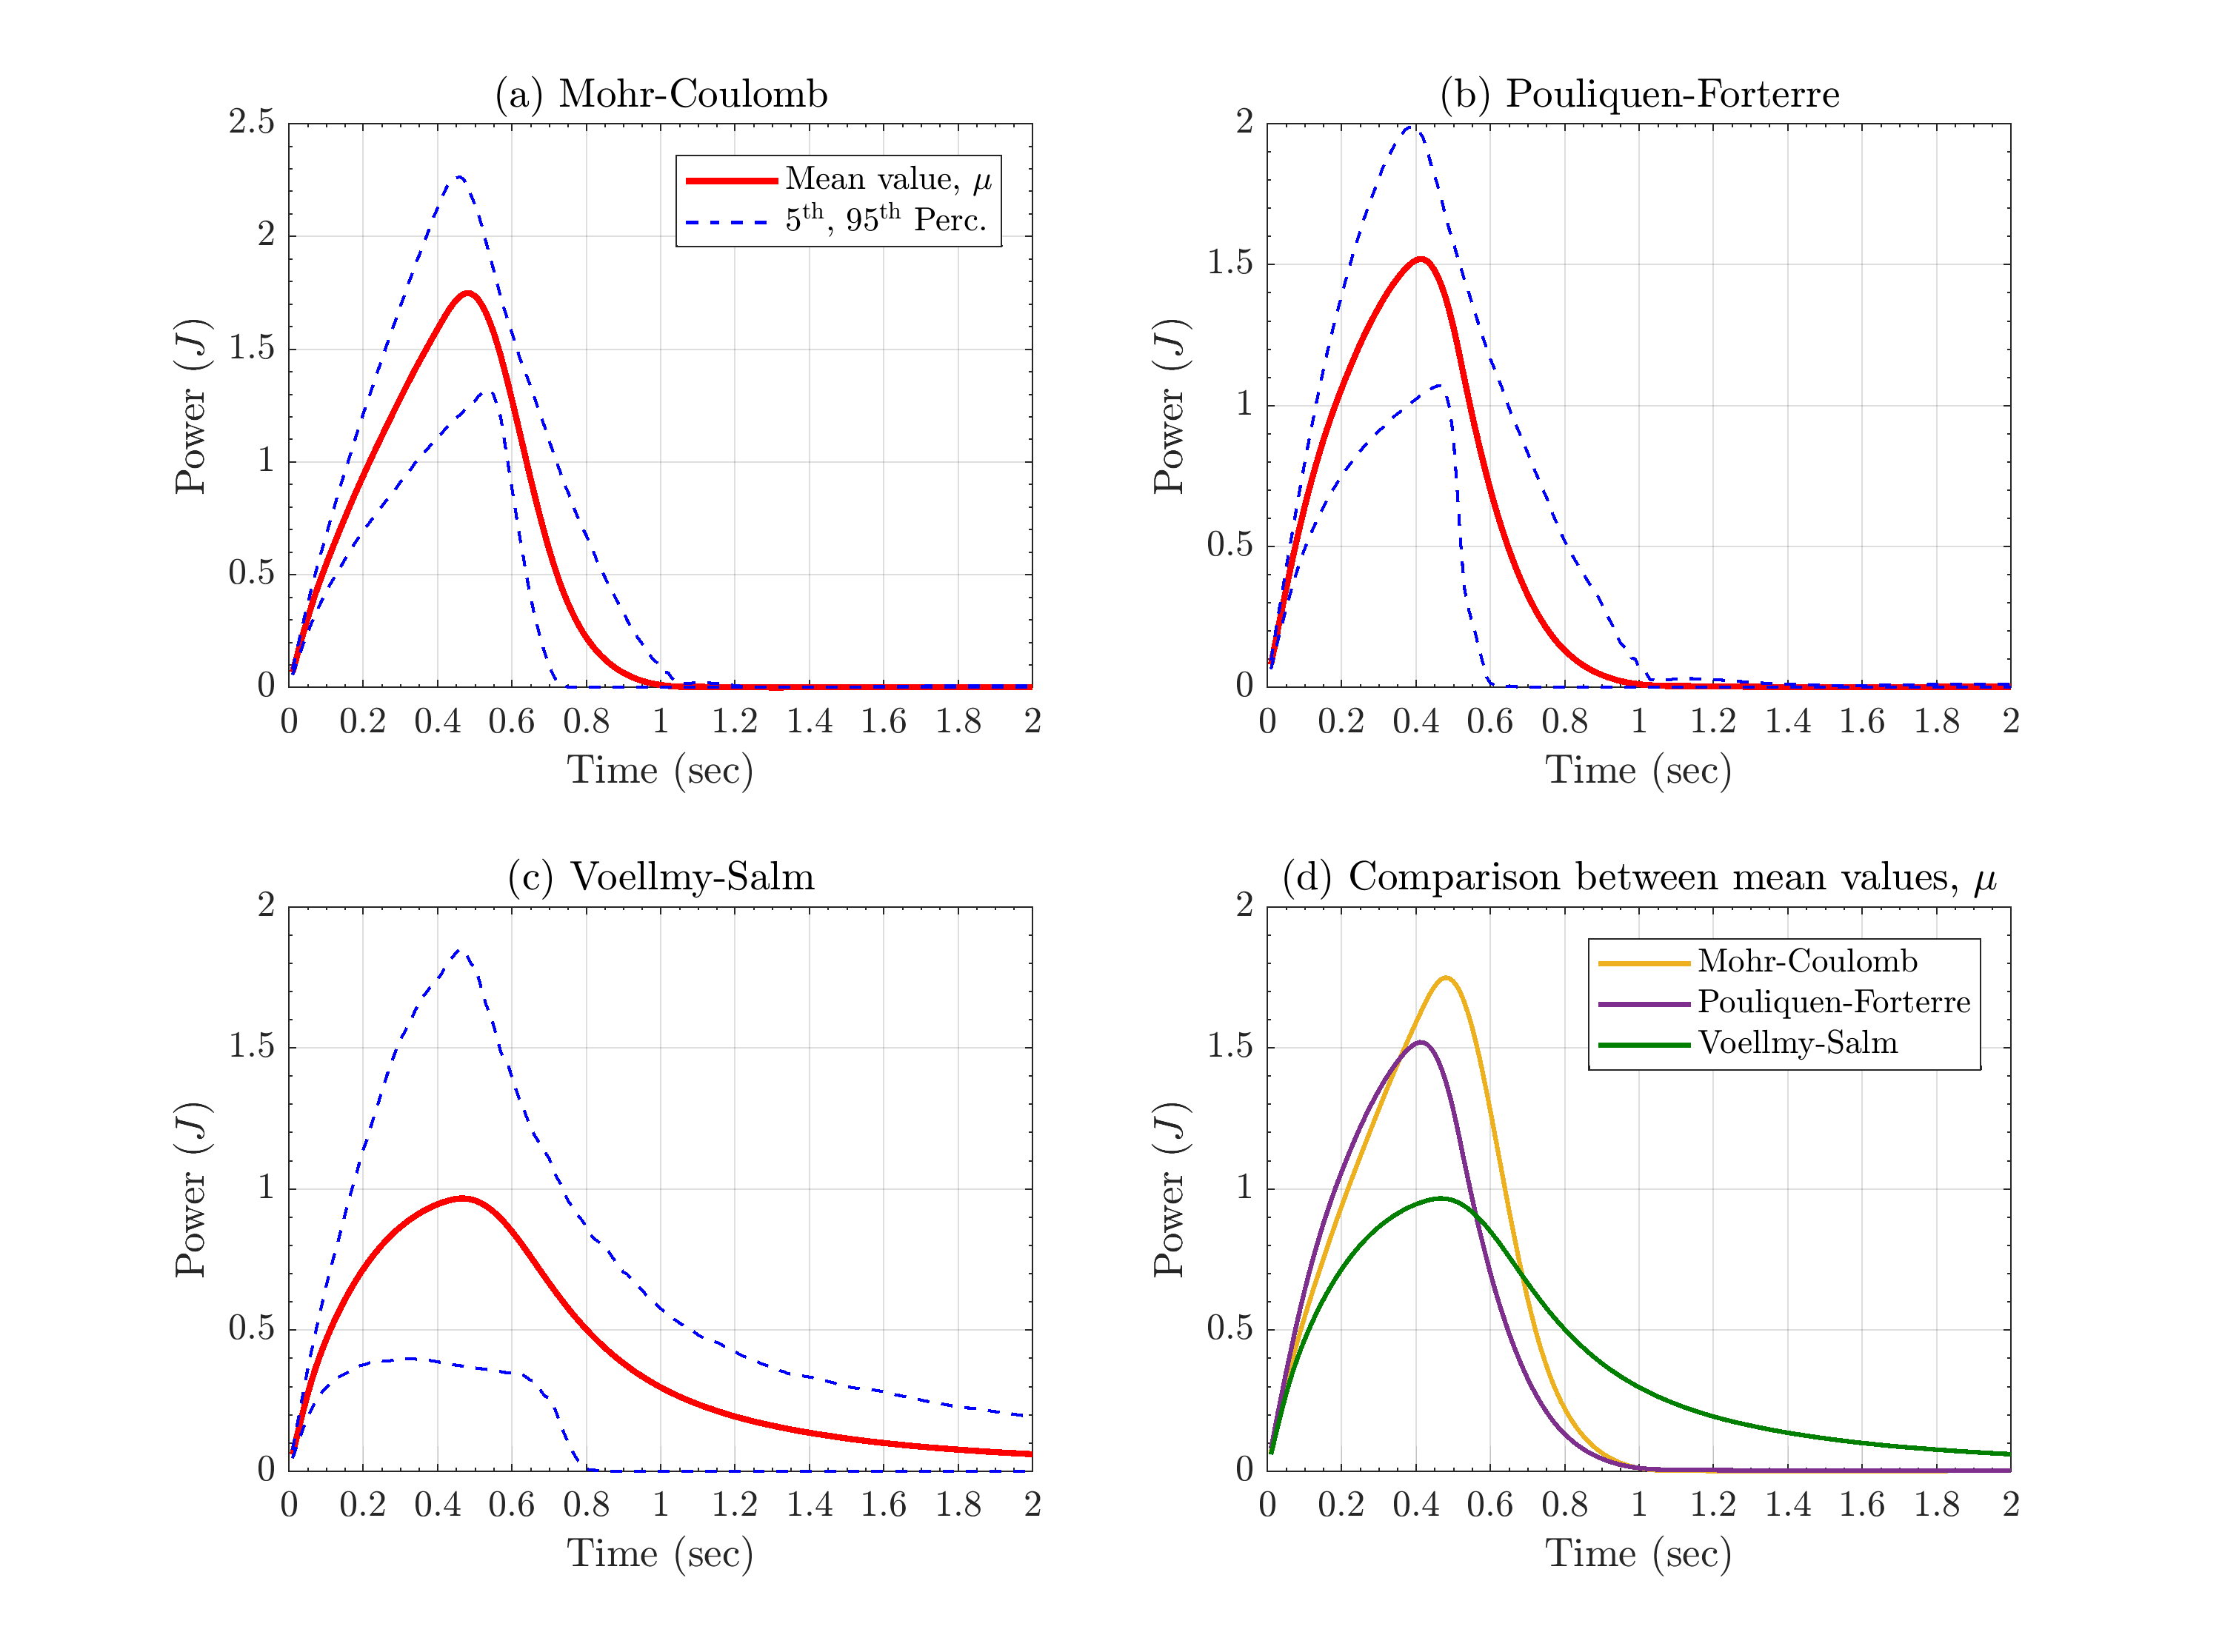
\includegraphics[width=1\textwidth]{InclinedPlane/Forces_Powers/RHS1/PRHS1.png}
        \caption{Comparison between mean values of flow acceleration (computed from LHS), $\Vert \underline{a} \Vert(L,t)$, recorded at locations of interest, $L_i, \ _{i=1,...,4}$.}
        \label{fig:Ramp-RHS1-Power-spatial}
\end{figure}

\newpage
\item	\textbf{RHS$_2$}

\begin{figure}[H]
        \centering
        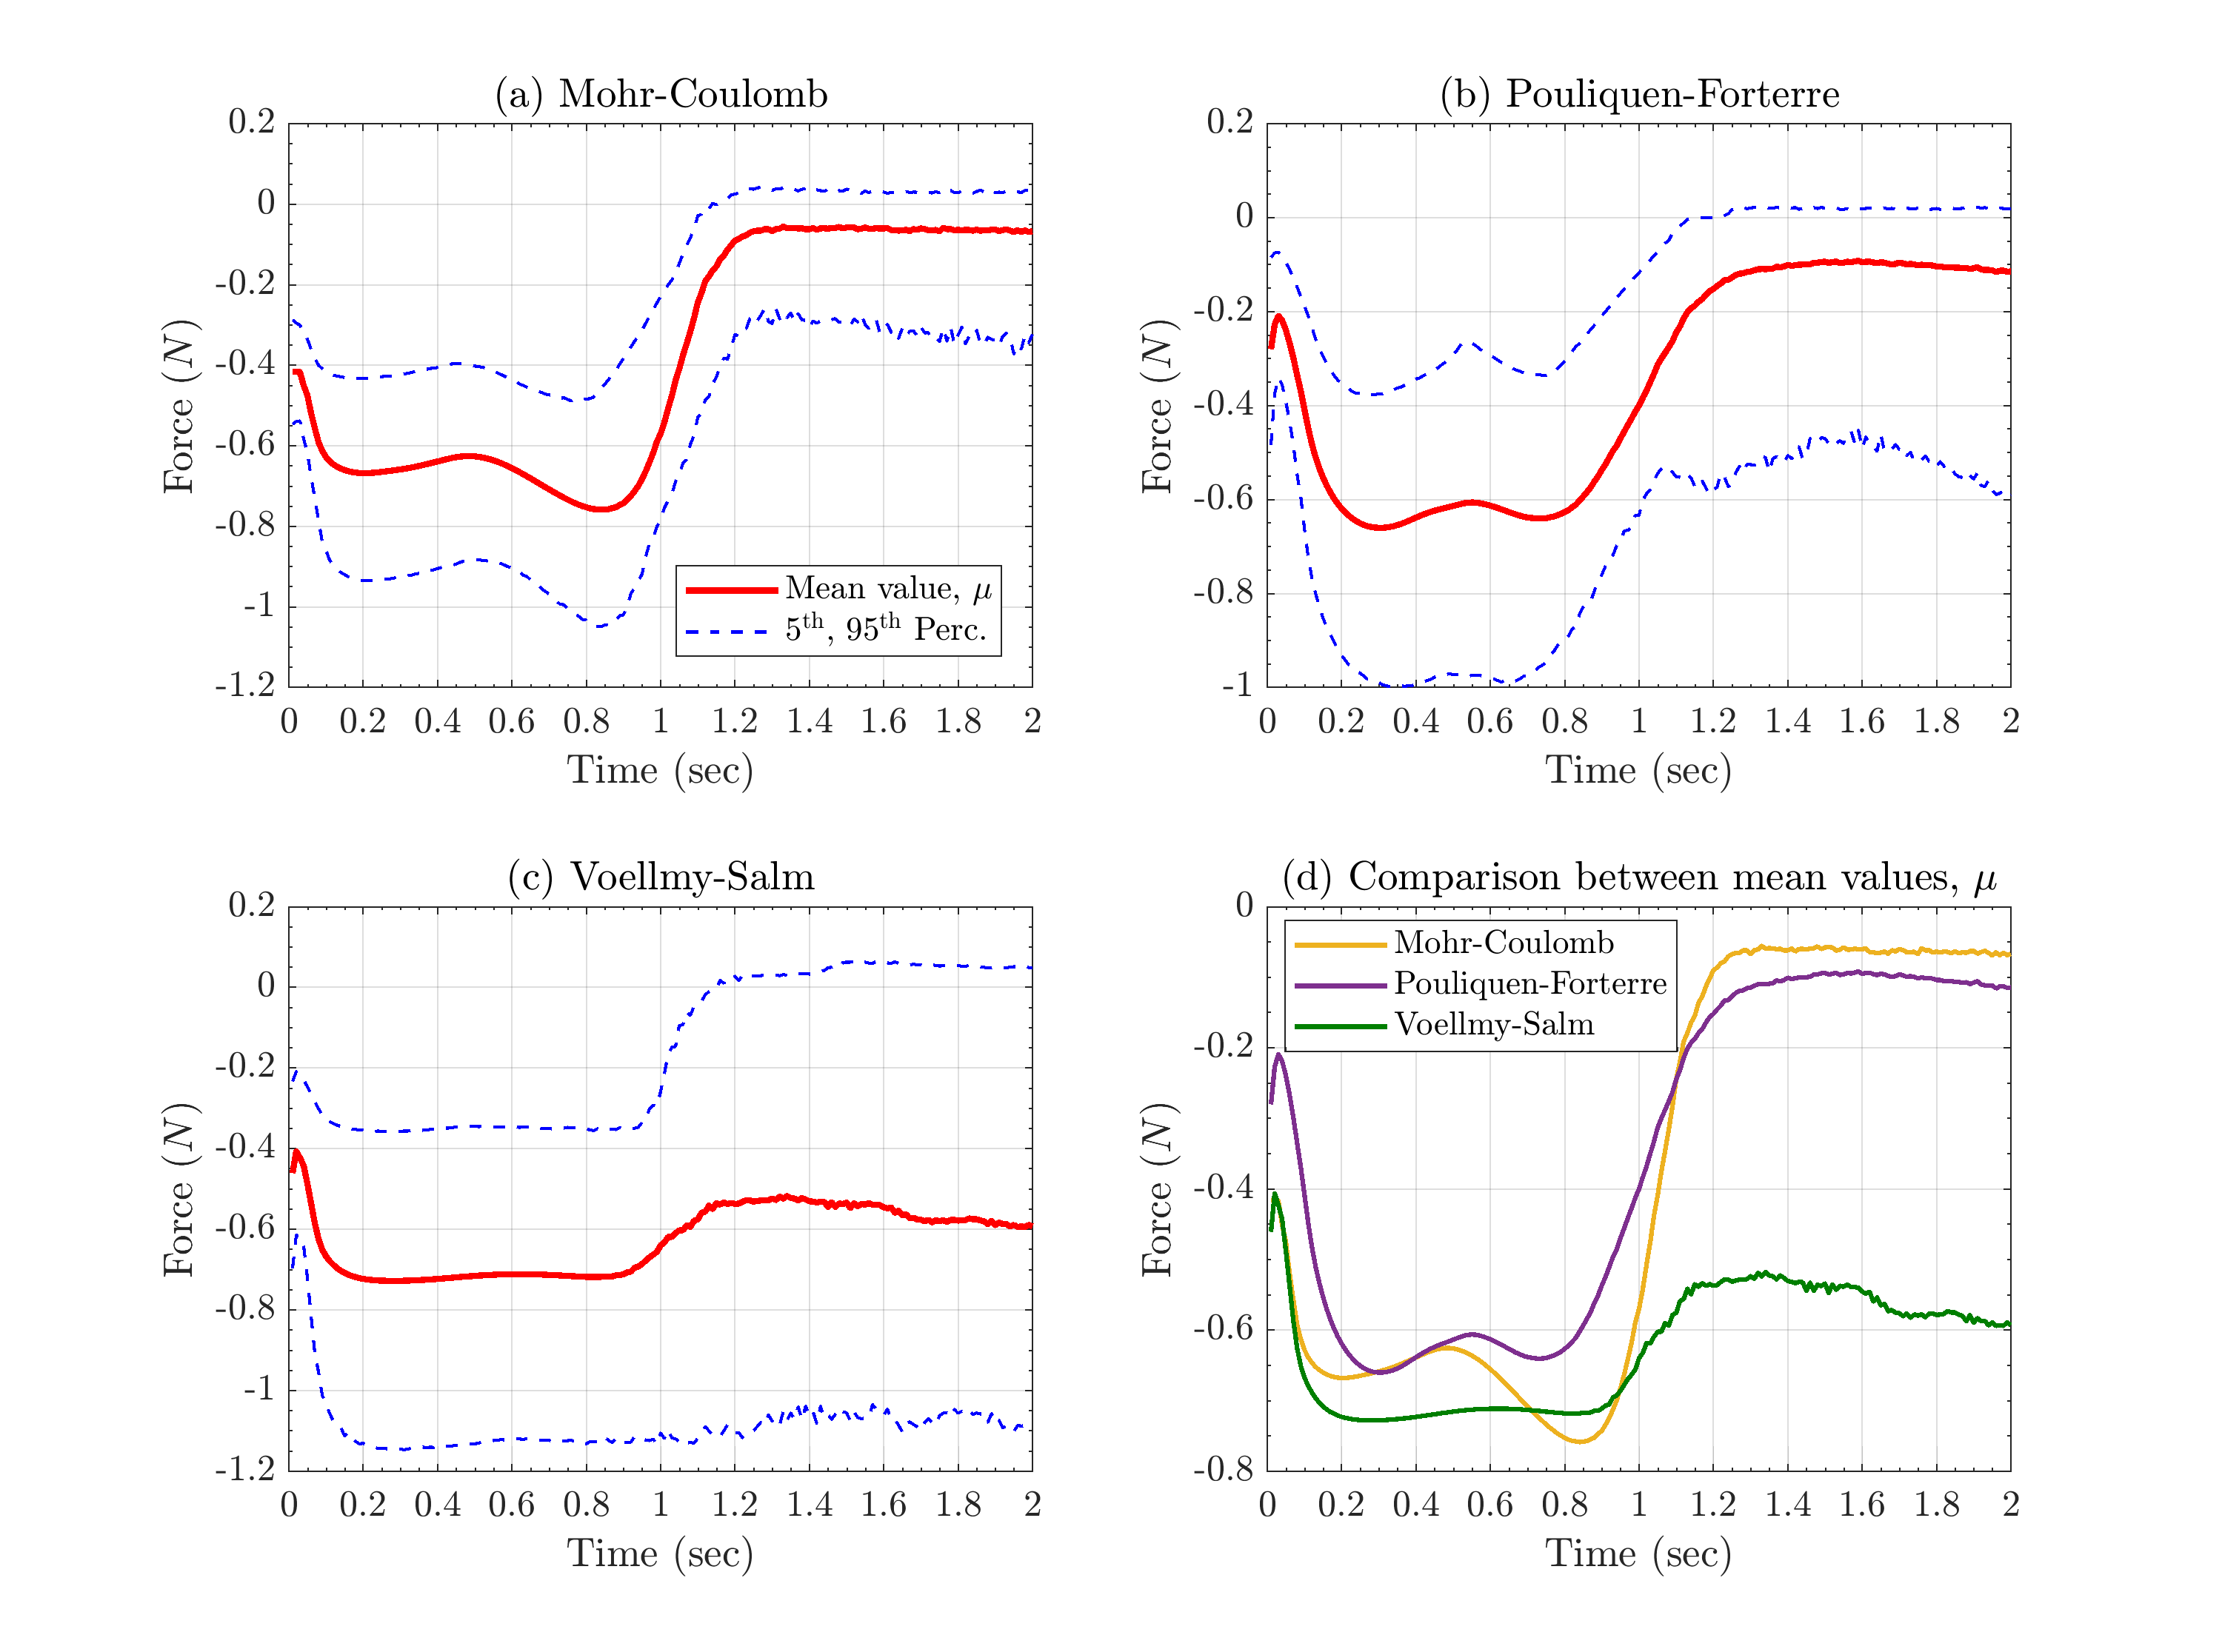
\includegraphics[width=1\textwidth]{InclinedPlane/Forces_Powers/RHS2/FRHS2x.png}
        \caption{Comparison between mean values of flow acceleration (computed from LHS), $\Vert \underline{a} \Vert(L,t)$, recorded at locations of interest, $L_i, \ _{i=1,...,4}$.}
        \label{fig:Ramp-RHS2-Fx-spatial}
\end{figure}

\begin{figure}[H]
        \centering
        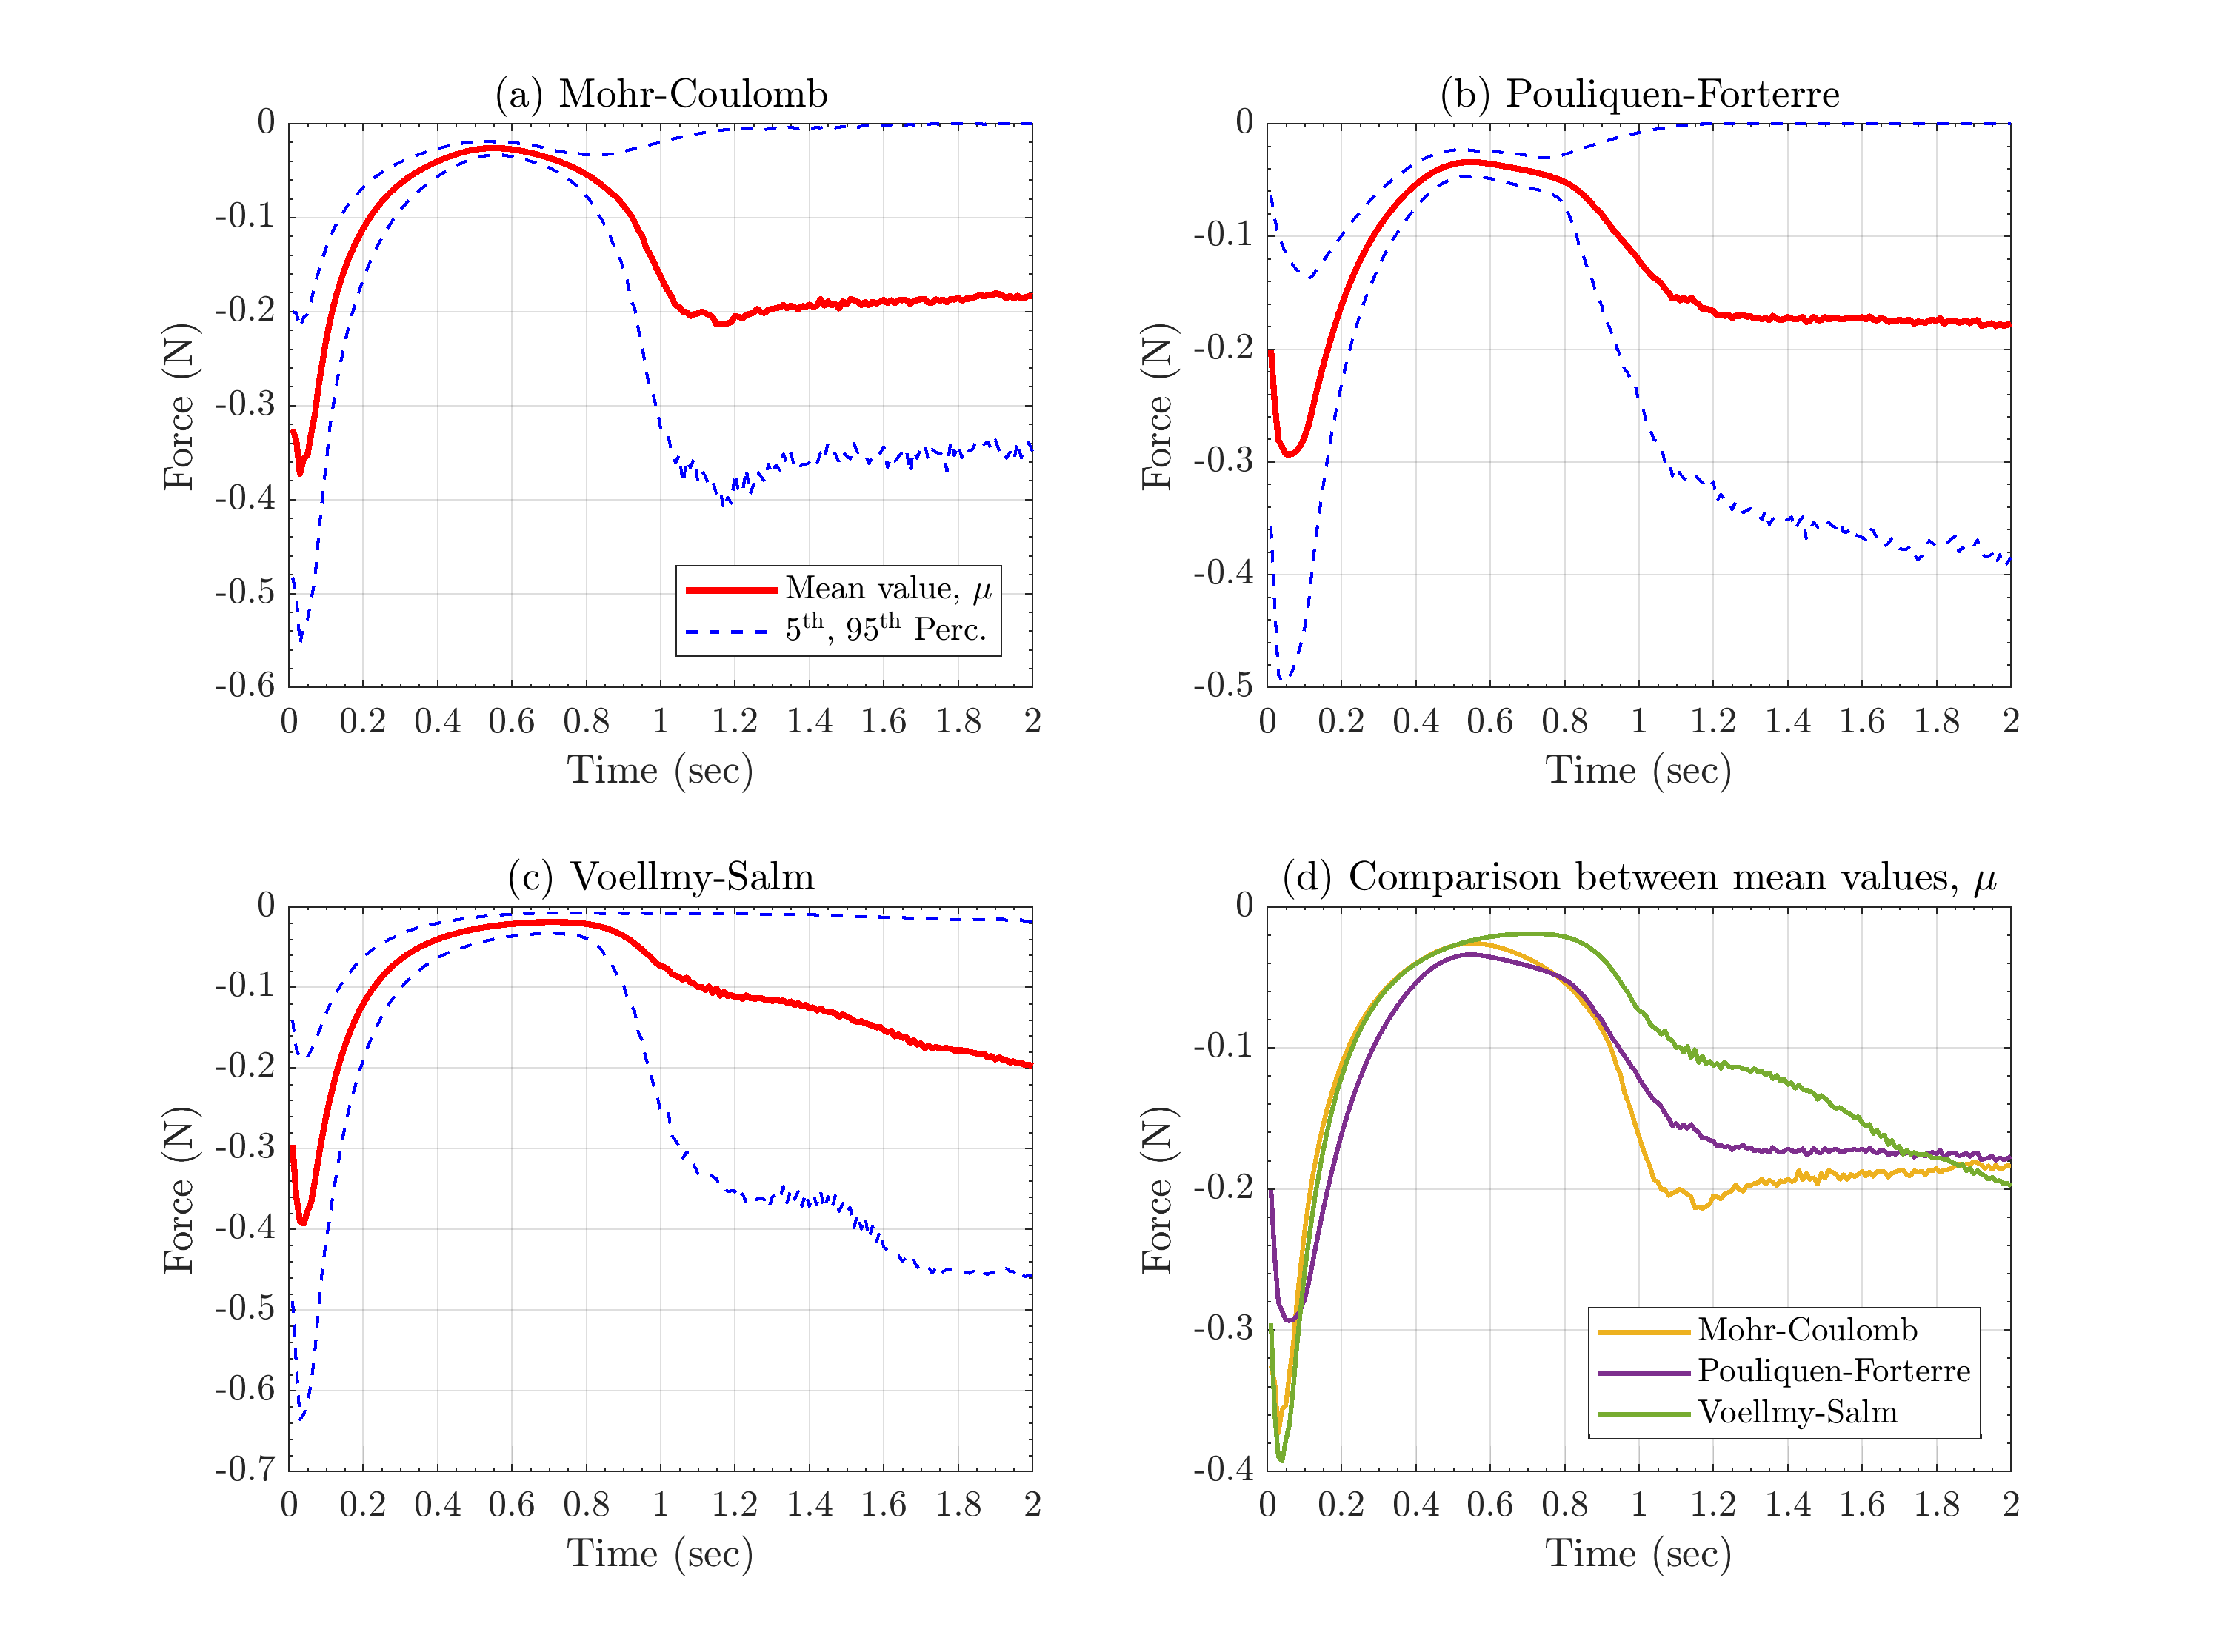
\includegraphics[width=1\textwidth]{InclinedPlane/Forces_Powers/RHS2/FRHS2y.png}
        \caption{Comparison between mean values of flow acceleration (computed from LHS), $\Vert \underline{a} \Vert(L,t)$, recorded at locations of interest, $L_i, \ _{i=1,...,4}$.}
        \label{fig:Ramp-RHS2-Fy-spatial}
\end{figure}

\begin{figure}[H]
        \centering
        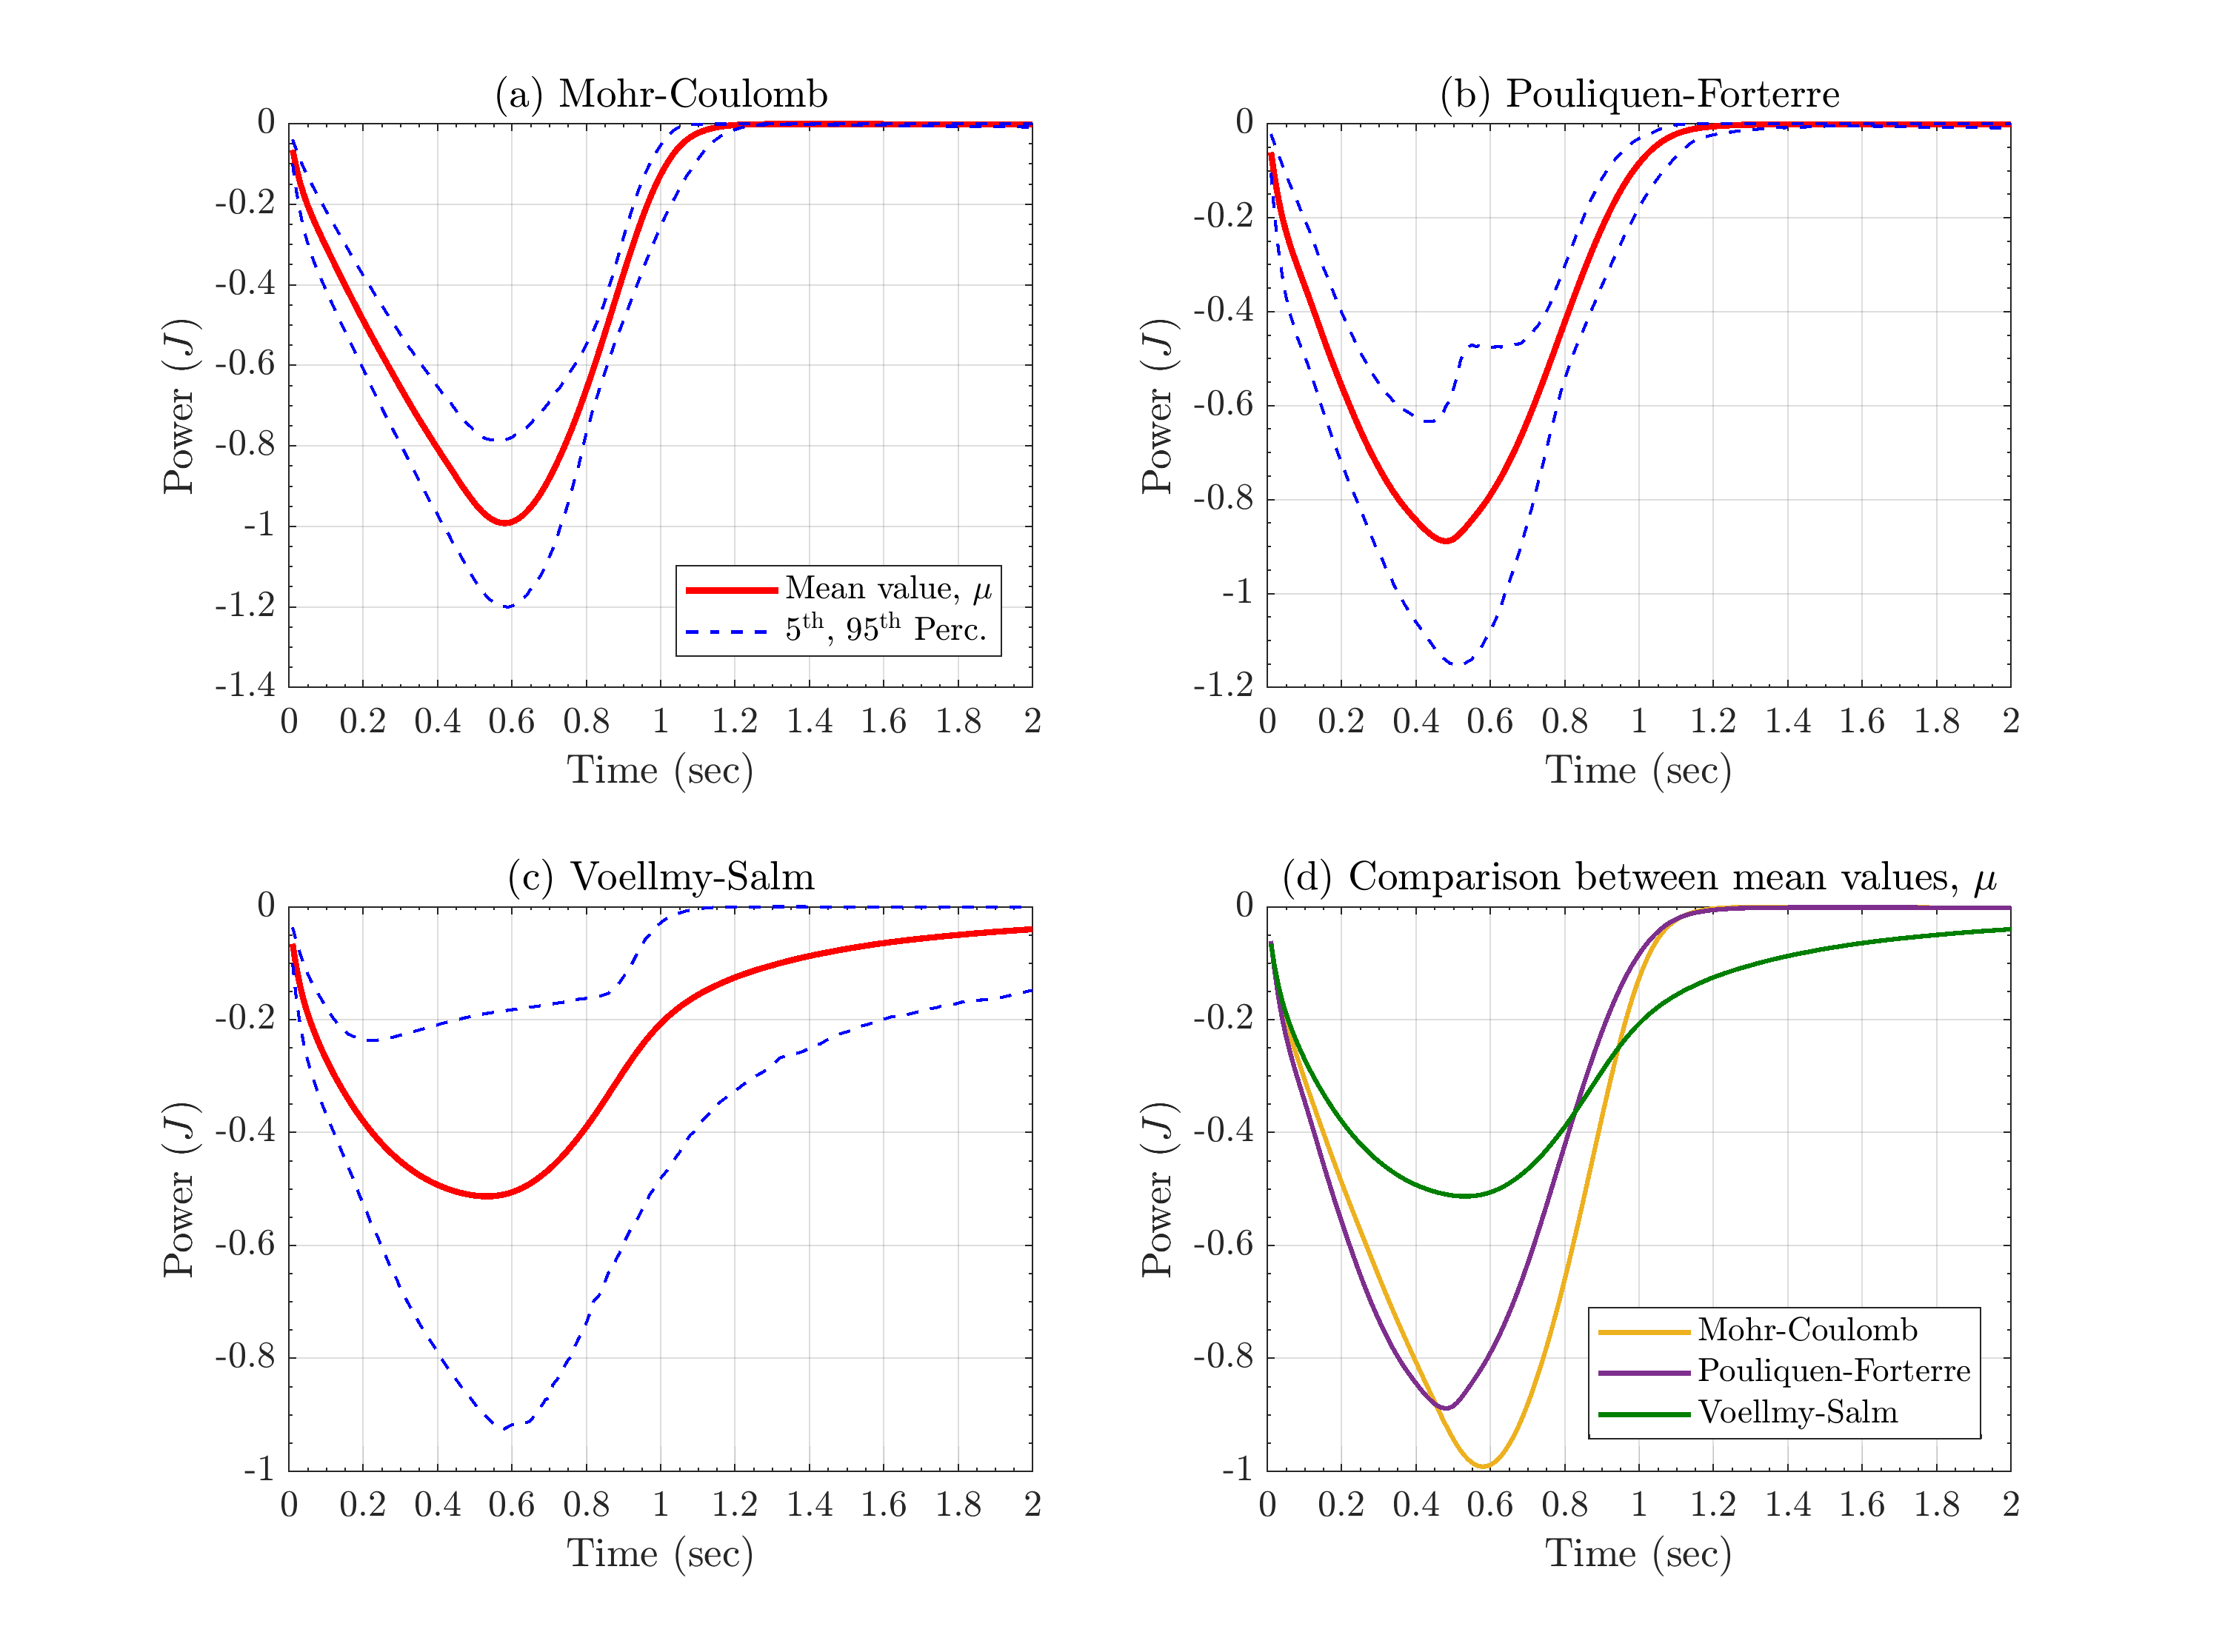
\includegraphics[width=1\textwidth]{InclinedPlane/Forces_Powers/RHS2/PRHS2.png}
        \caption{Comparison between mean values of flow acceleration (computed from LHS), $\Vert \underline{a} \Vert(L,t)$, recorded at locations of interest, $L_i, \ _{i=1,...,4}$.}
        \label{fig:Ramp-RHS2-Power-spatial}
\end{figure}

\newpage
\item	\textbf{RHS$_3$}

\begin{figure}[H]
        \centering
        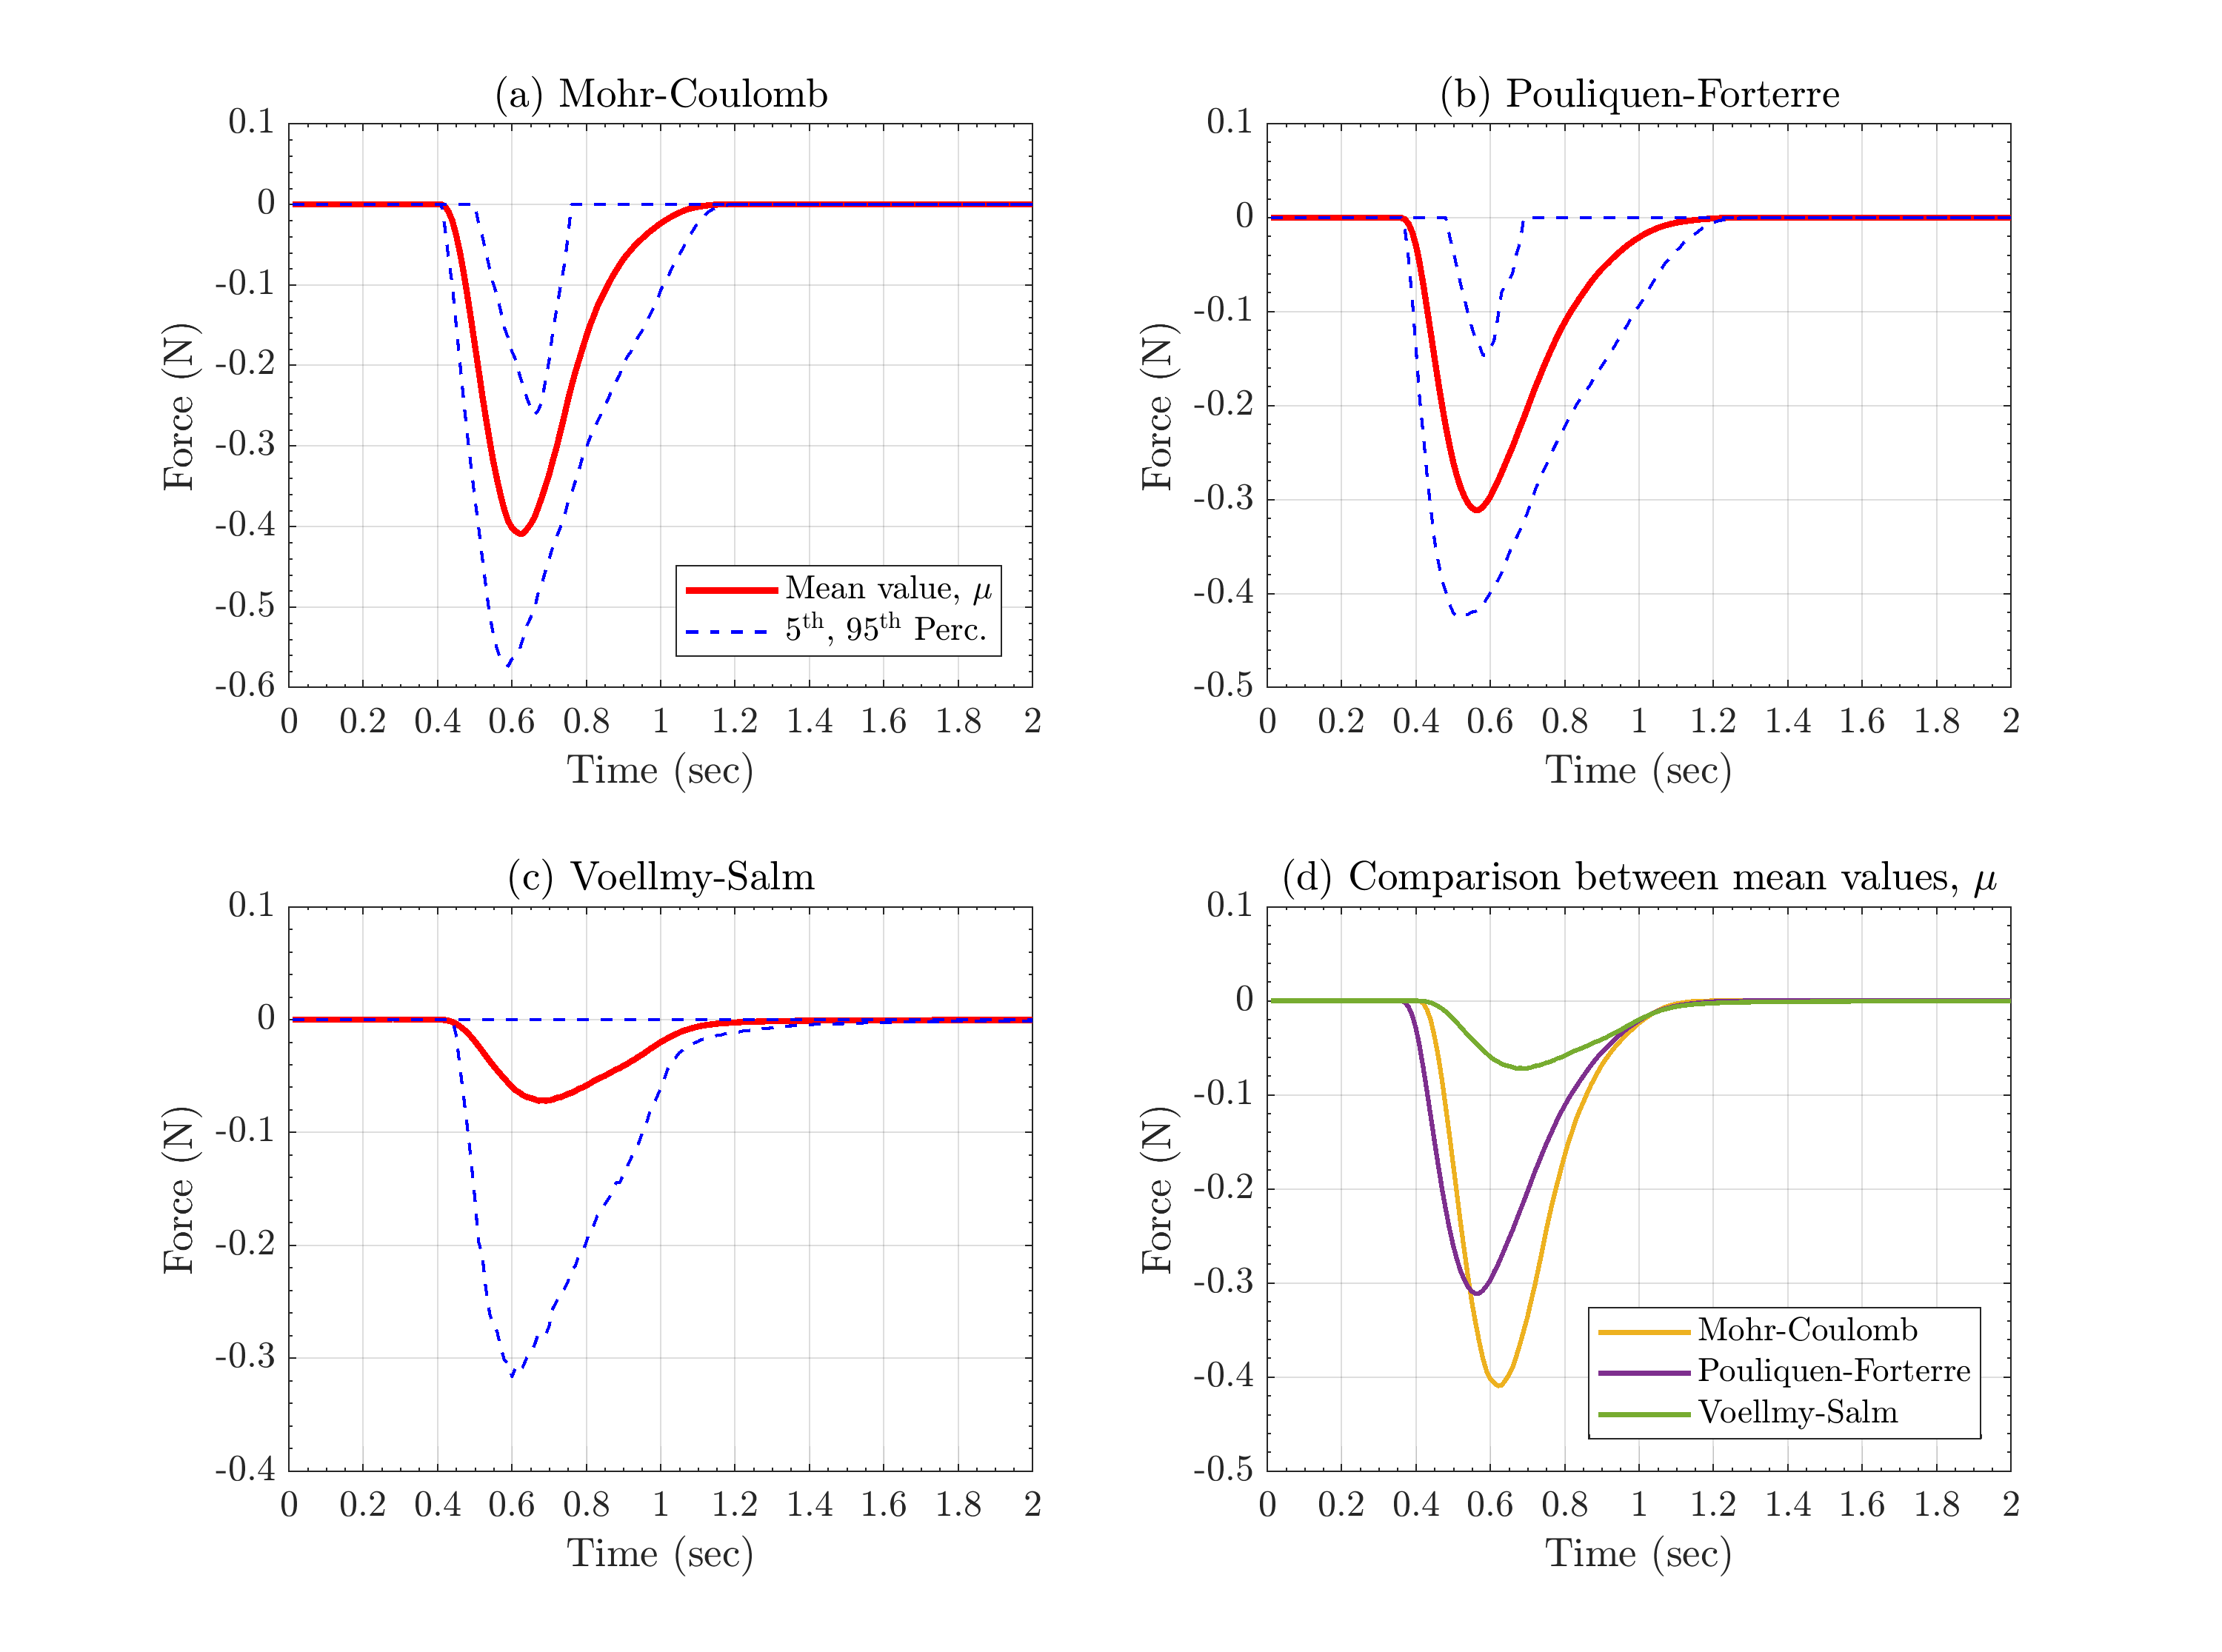
\includegraphics[width=1\textwidth]{InclinedPlane/Forces_Powers/RHS3/FRHS3x.png}
        \caption{Comparison between mean values of flow acceleration (computed from LHS), $\Vert \underline{a} \Vert(L,t)$, recorded at locations of interest, $L_i, \ _{i=1,...,4}$.}
        \label{fig:Ramp-RHS3-Fx-spatial}
\end{figure}

\begin{figure}[H]
        \centering
        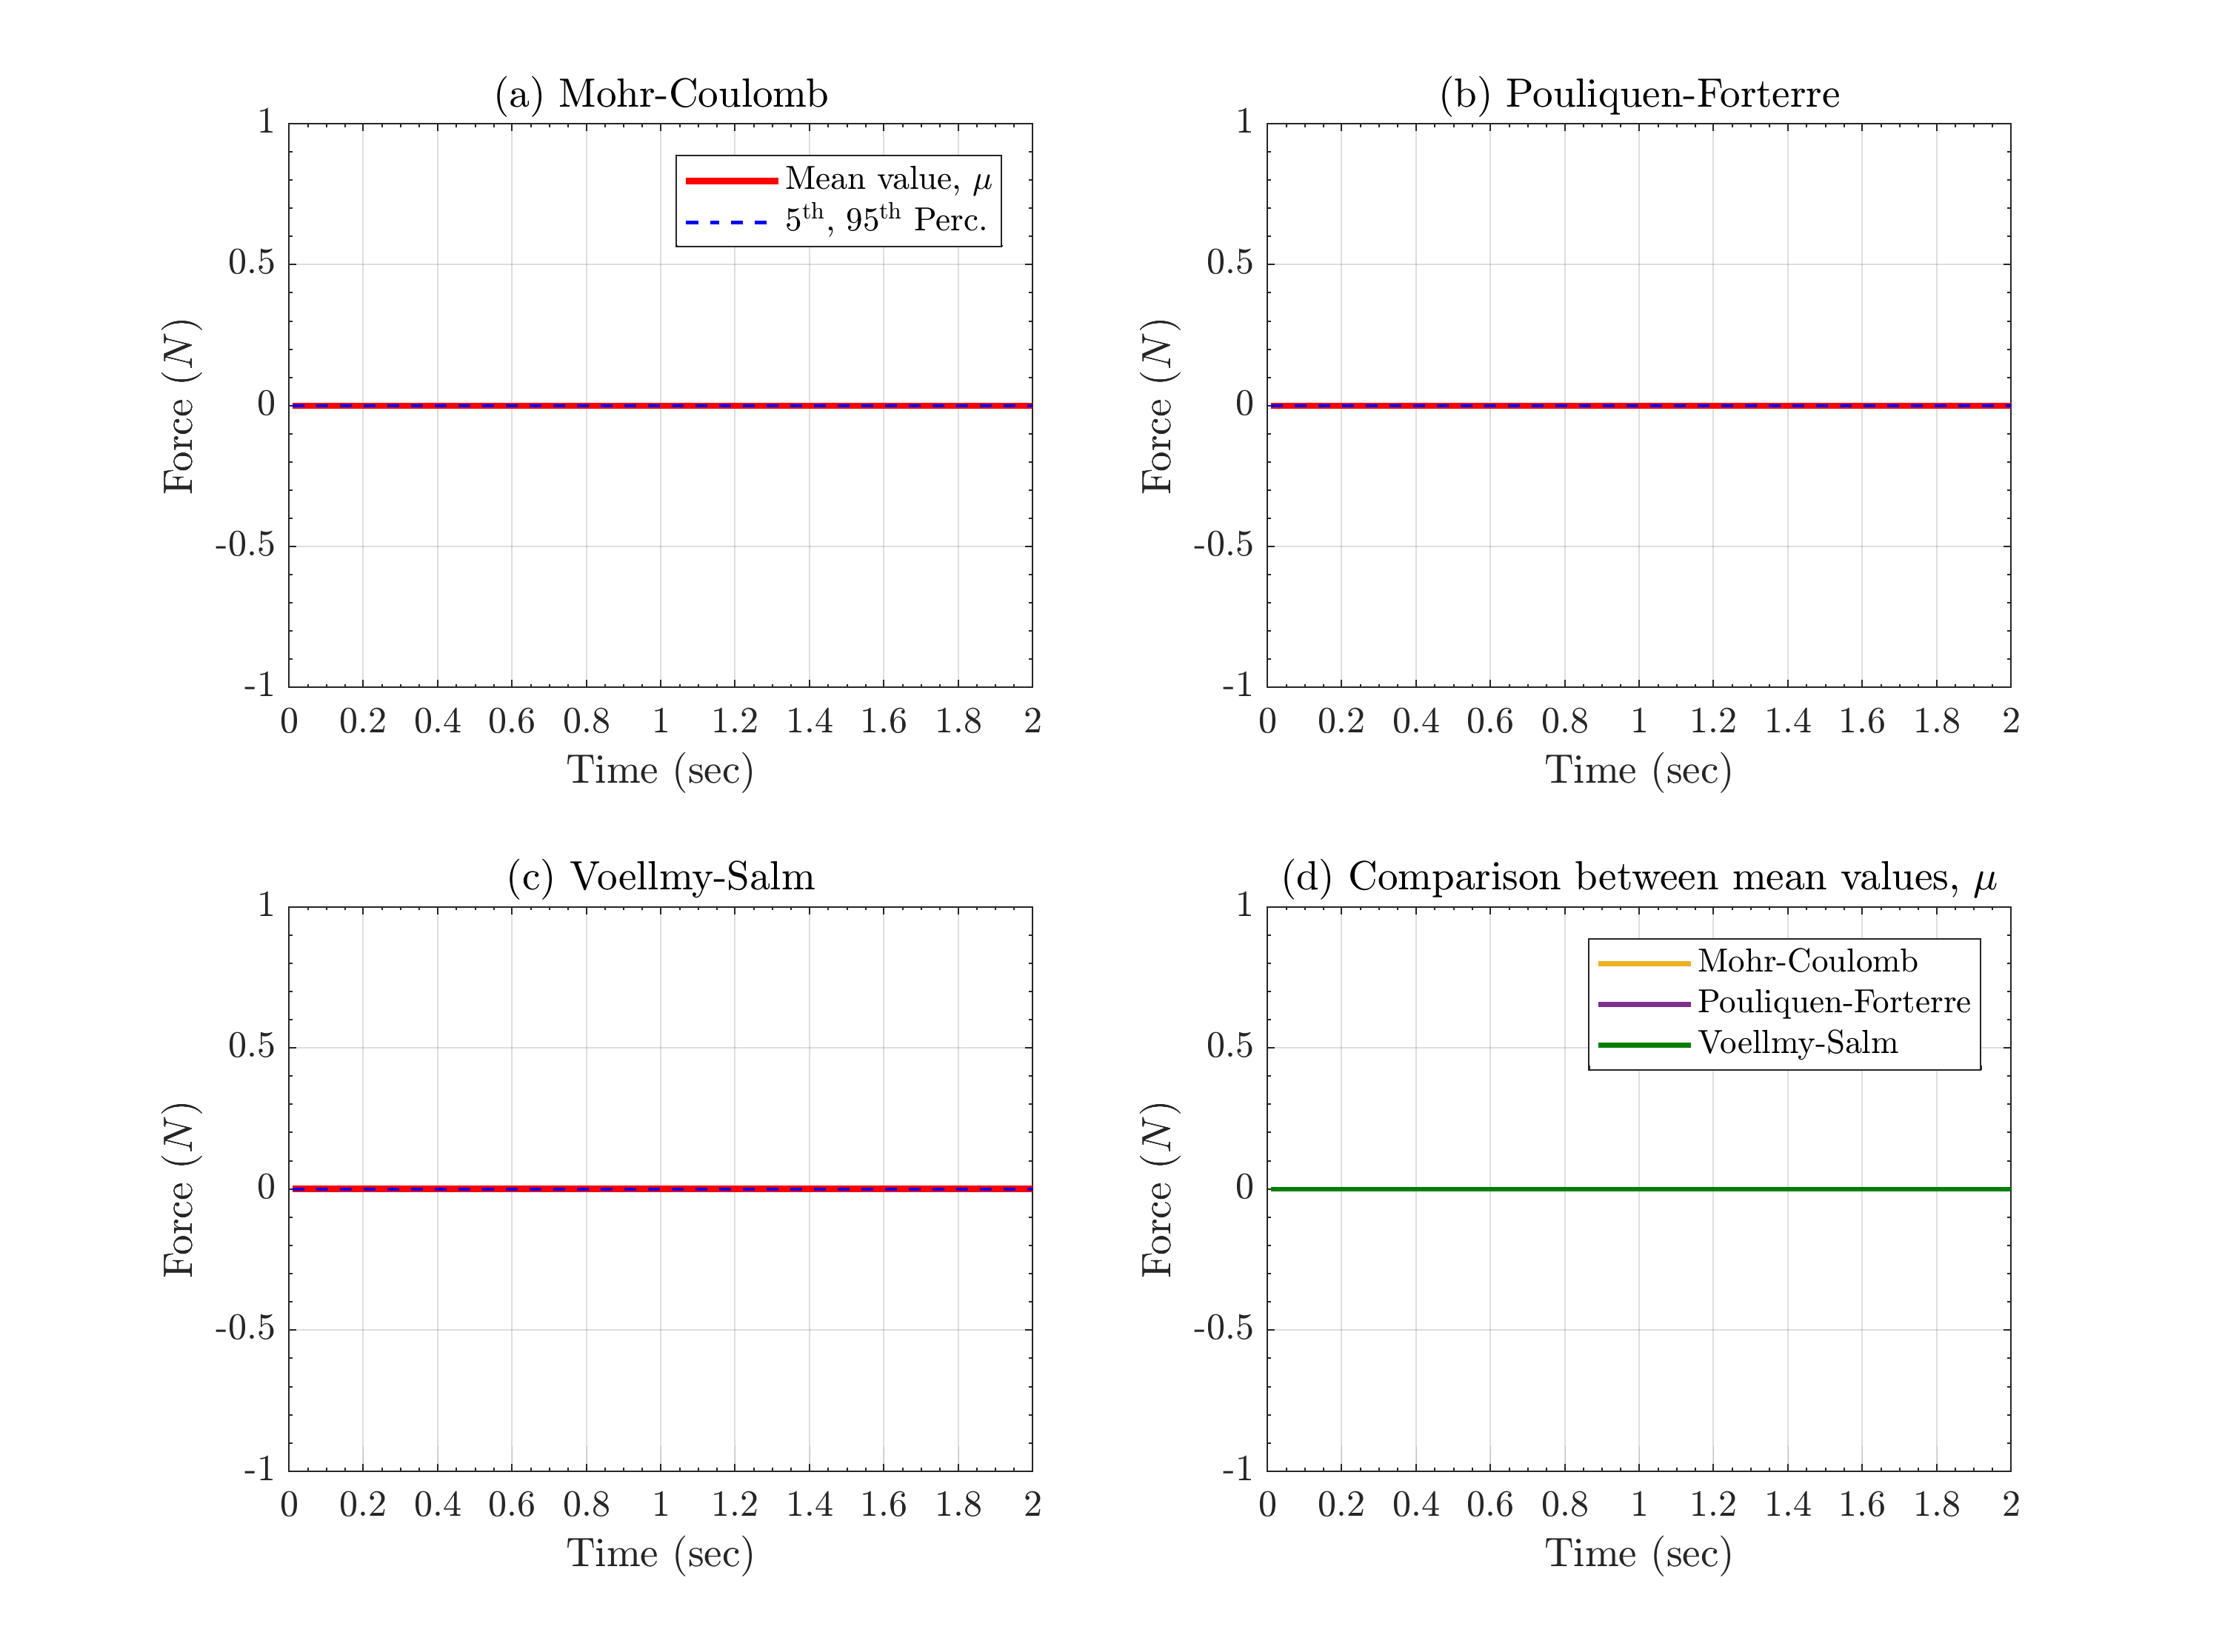
\includegraphics[width=1\textwidth]{InclinedPlane/Forces_Powers/RHS3/FRHS3y.png}
        \caption{Comparison between mean values of flow acceleration (computed from LHS), $\Vert \underline{a} \Vert(L,t)$, recorded at locations of interest, $L_i, \ _{i=1,...,4}$.}
        \label{fig:Ramp-RHS3-Fy-spatial}
\end{figure}

\begin{figure}[H]
        \centering
        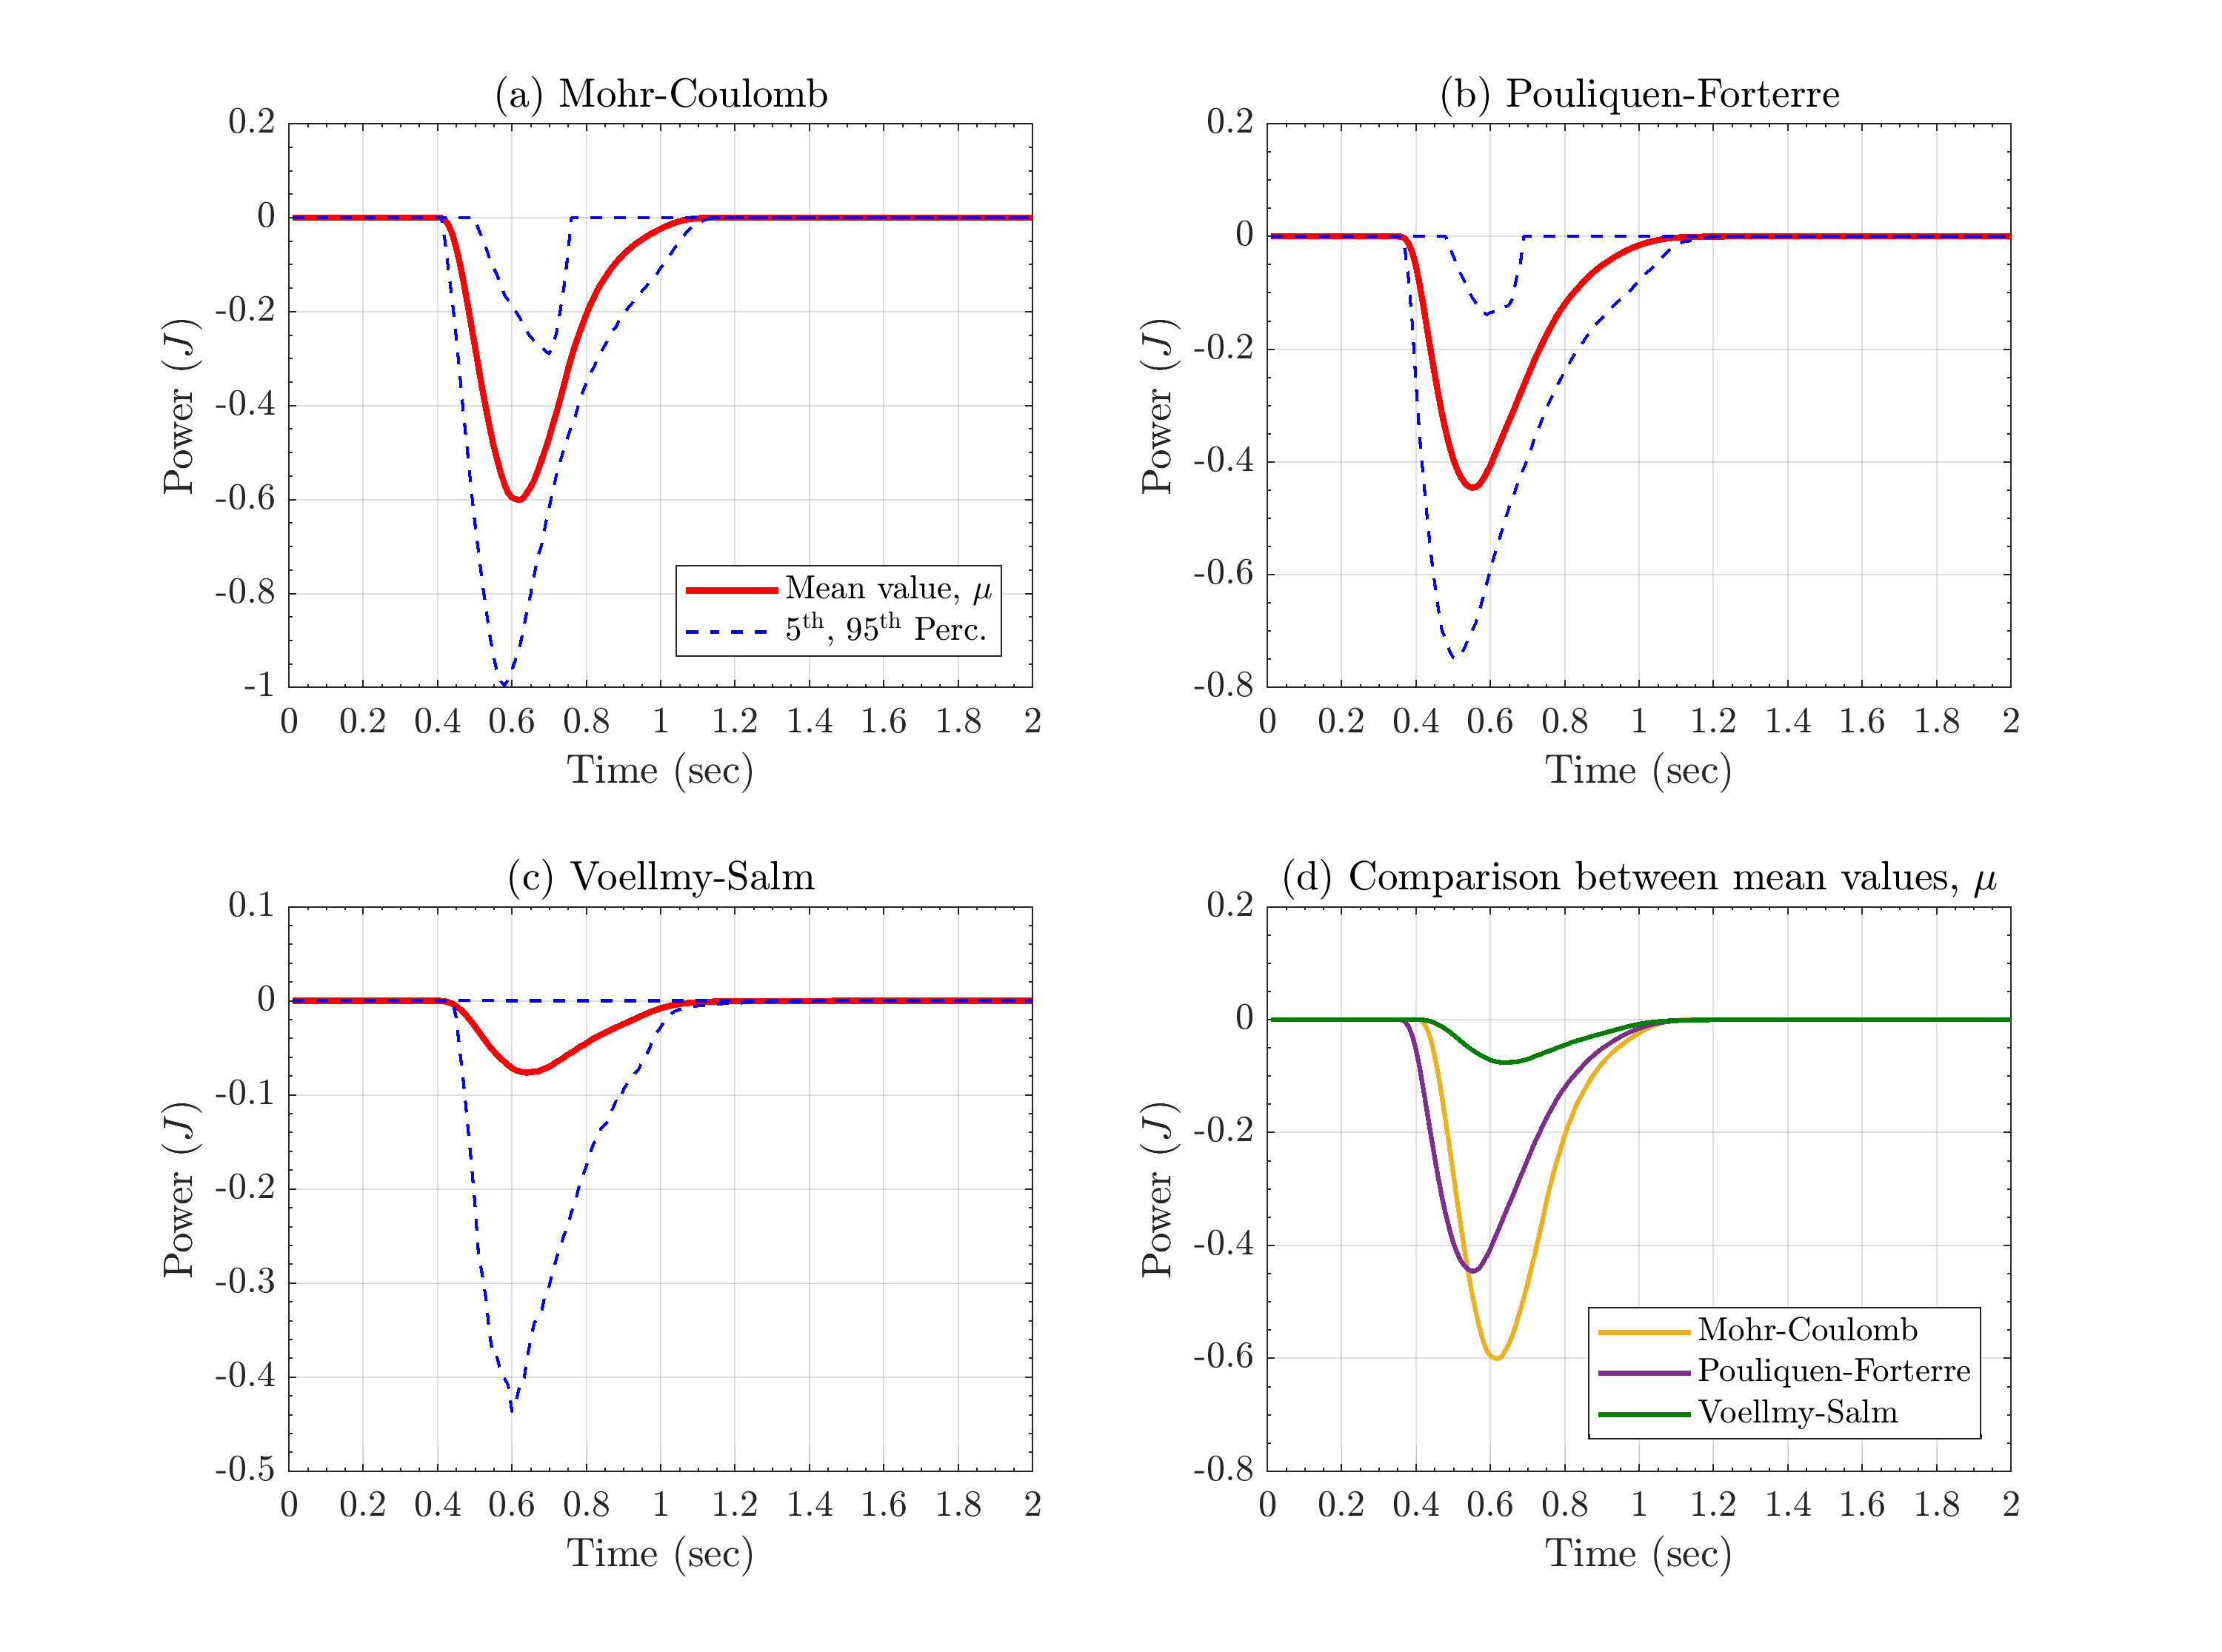
\includegraphics[width=1\textwidth]{InclinedPlane/Forces_Powers/RHS3/PRHS3.png}
        \caption{Comparison between mean values of flow acceleration (computed from LHS), $\Vert \underline{a} \Vert(L,t)$, recorded at locations of interest, $L_i, \ _{i=1,...,4}$.}
        \label{fig:Ramp-RHS3-Power-spatial}
\end{figure}

\newpage
\item	\textbf{RHS$_4$}

\begin{figure}[H]
        \centering
        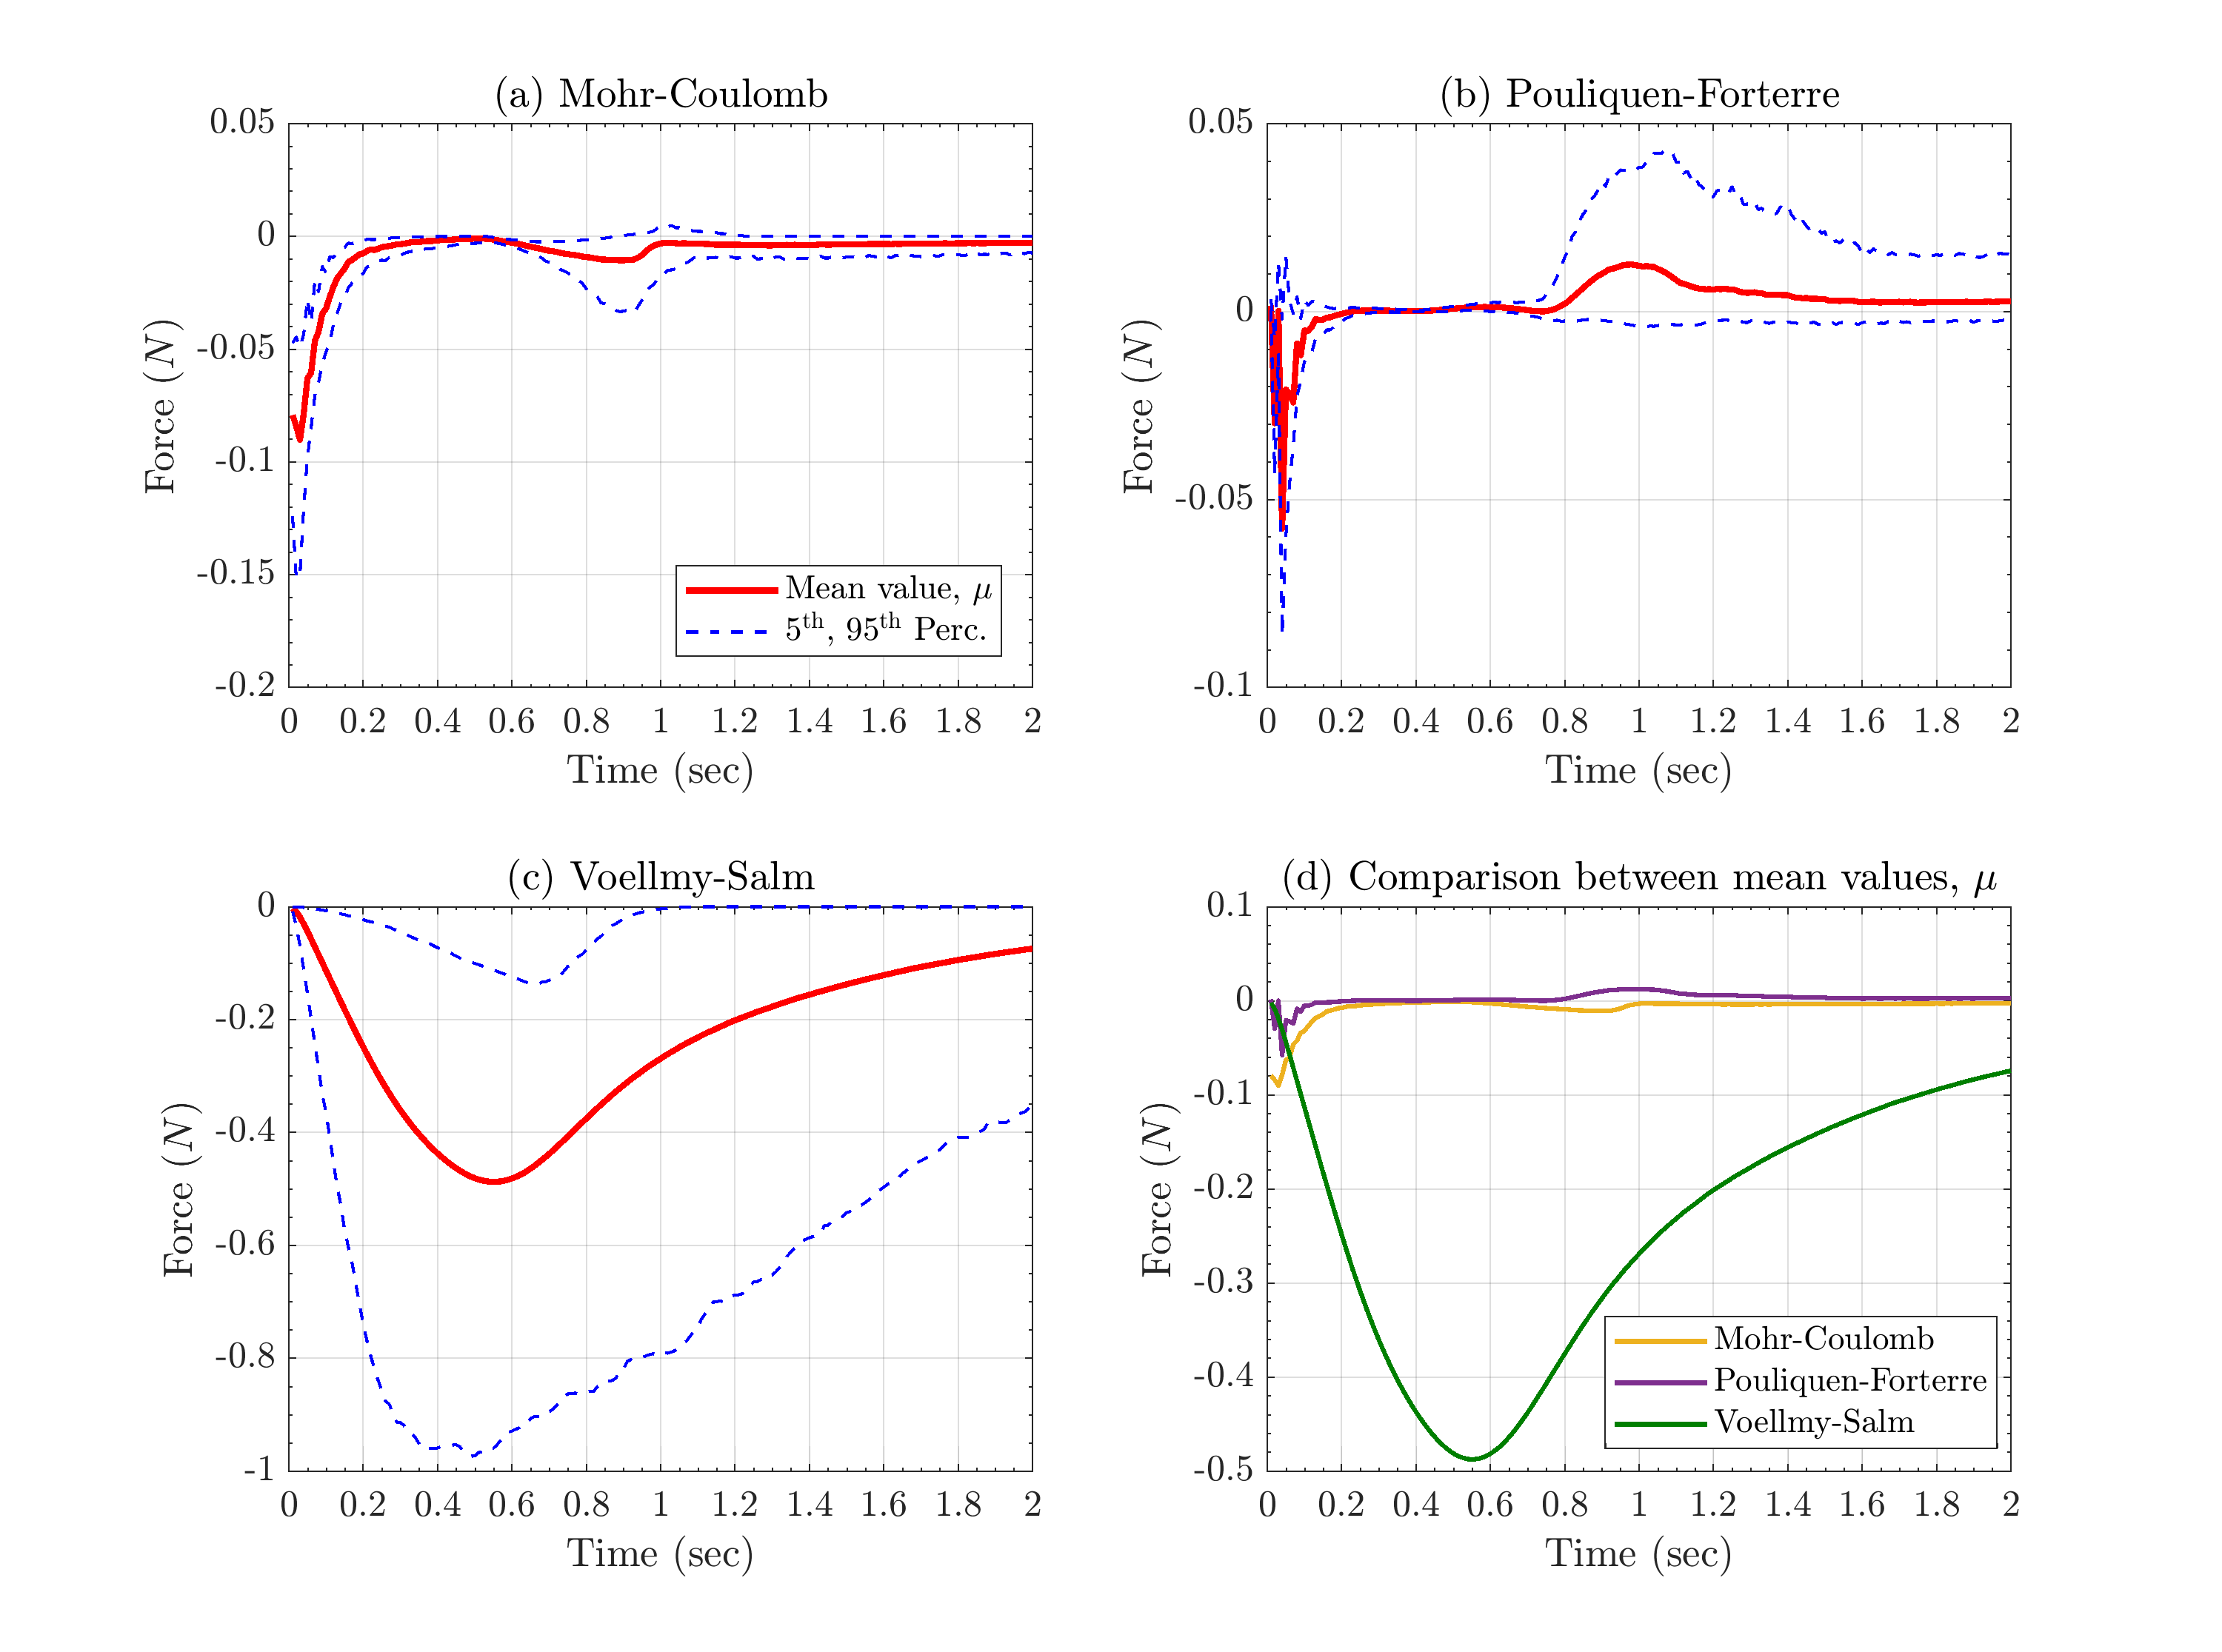
\includegraphics[width=1\textwidth]{InclinedPlane/Forces_Powers/RHS4/FRHS4x.png}
        \caption{Comparison between mean values of flow acceleration (computed from LHS), $\Vert \underline{a} \Vert(L,t)$, recorded at locations of interest, $L_i, \ _{i=1,...,4}$.}
        \label{fig:Ramp-RHS4-Fx-spatial}
\end{figure}

\begin{figure}[H]
        \centering
        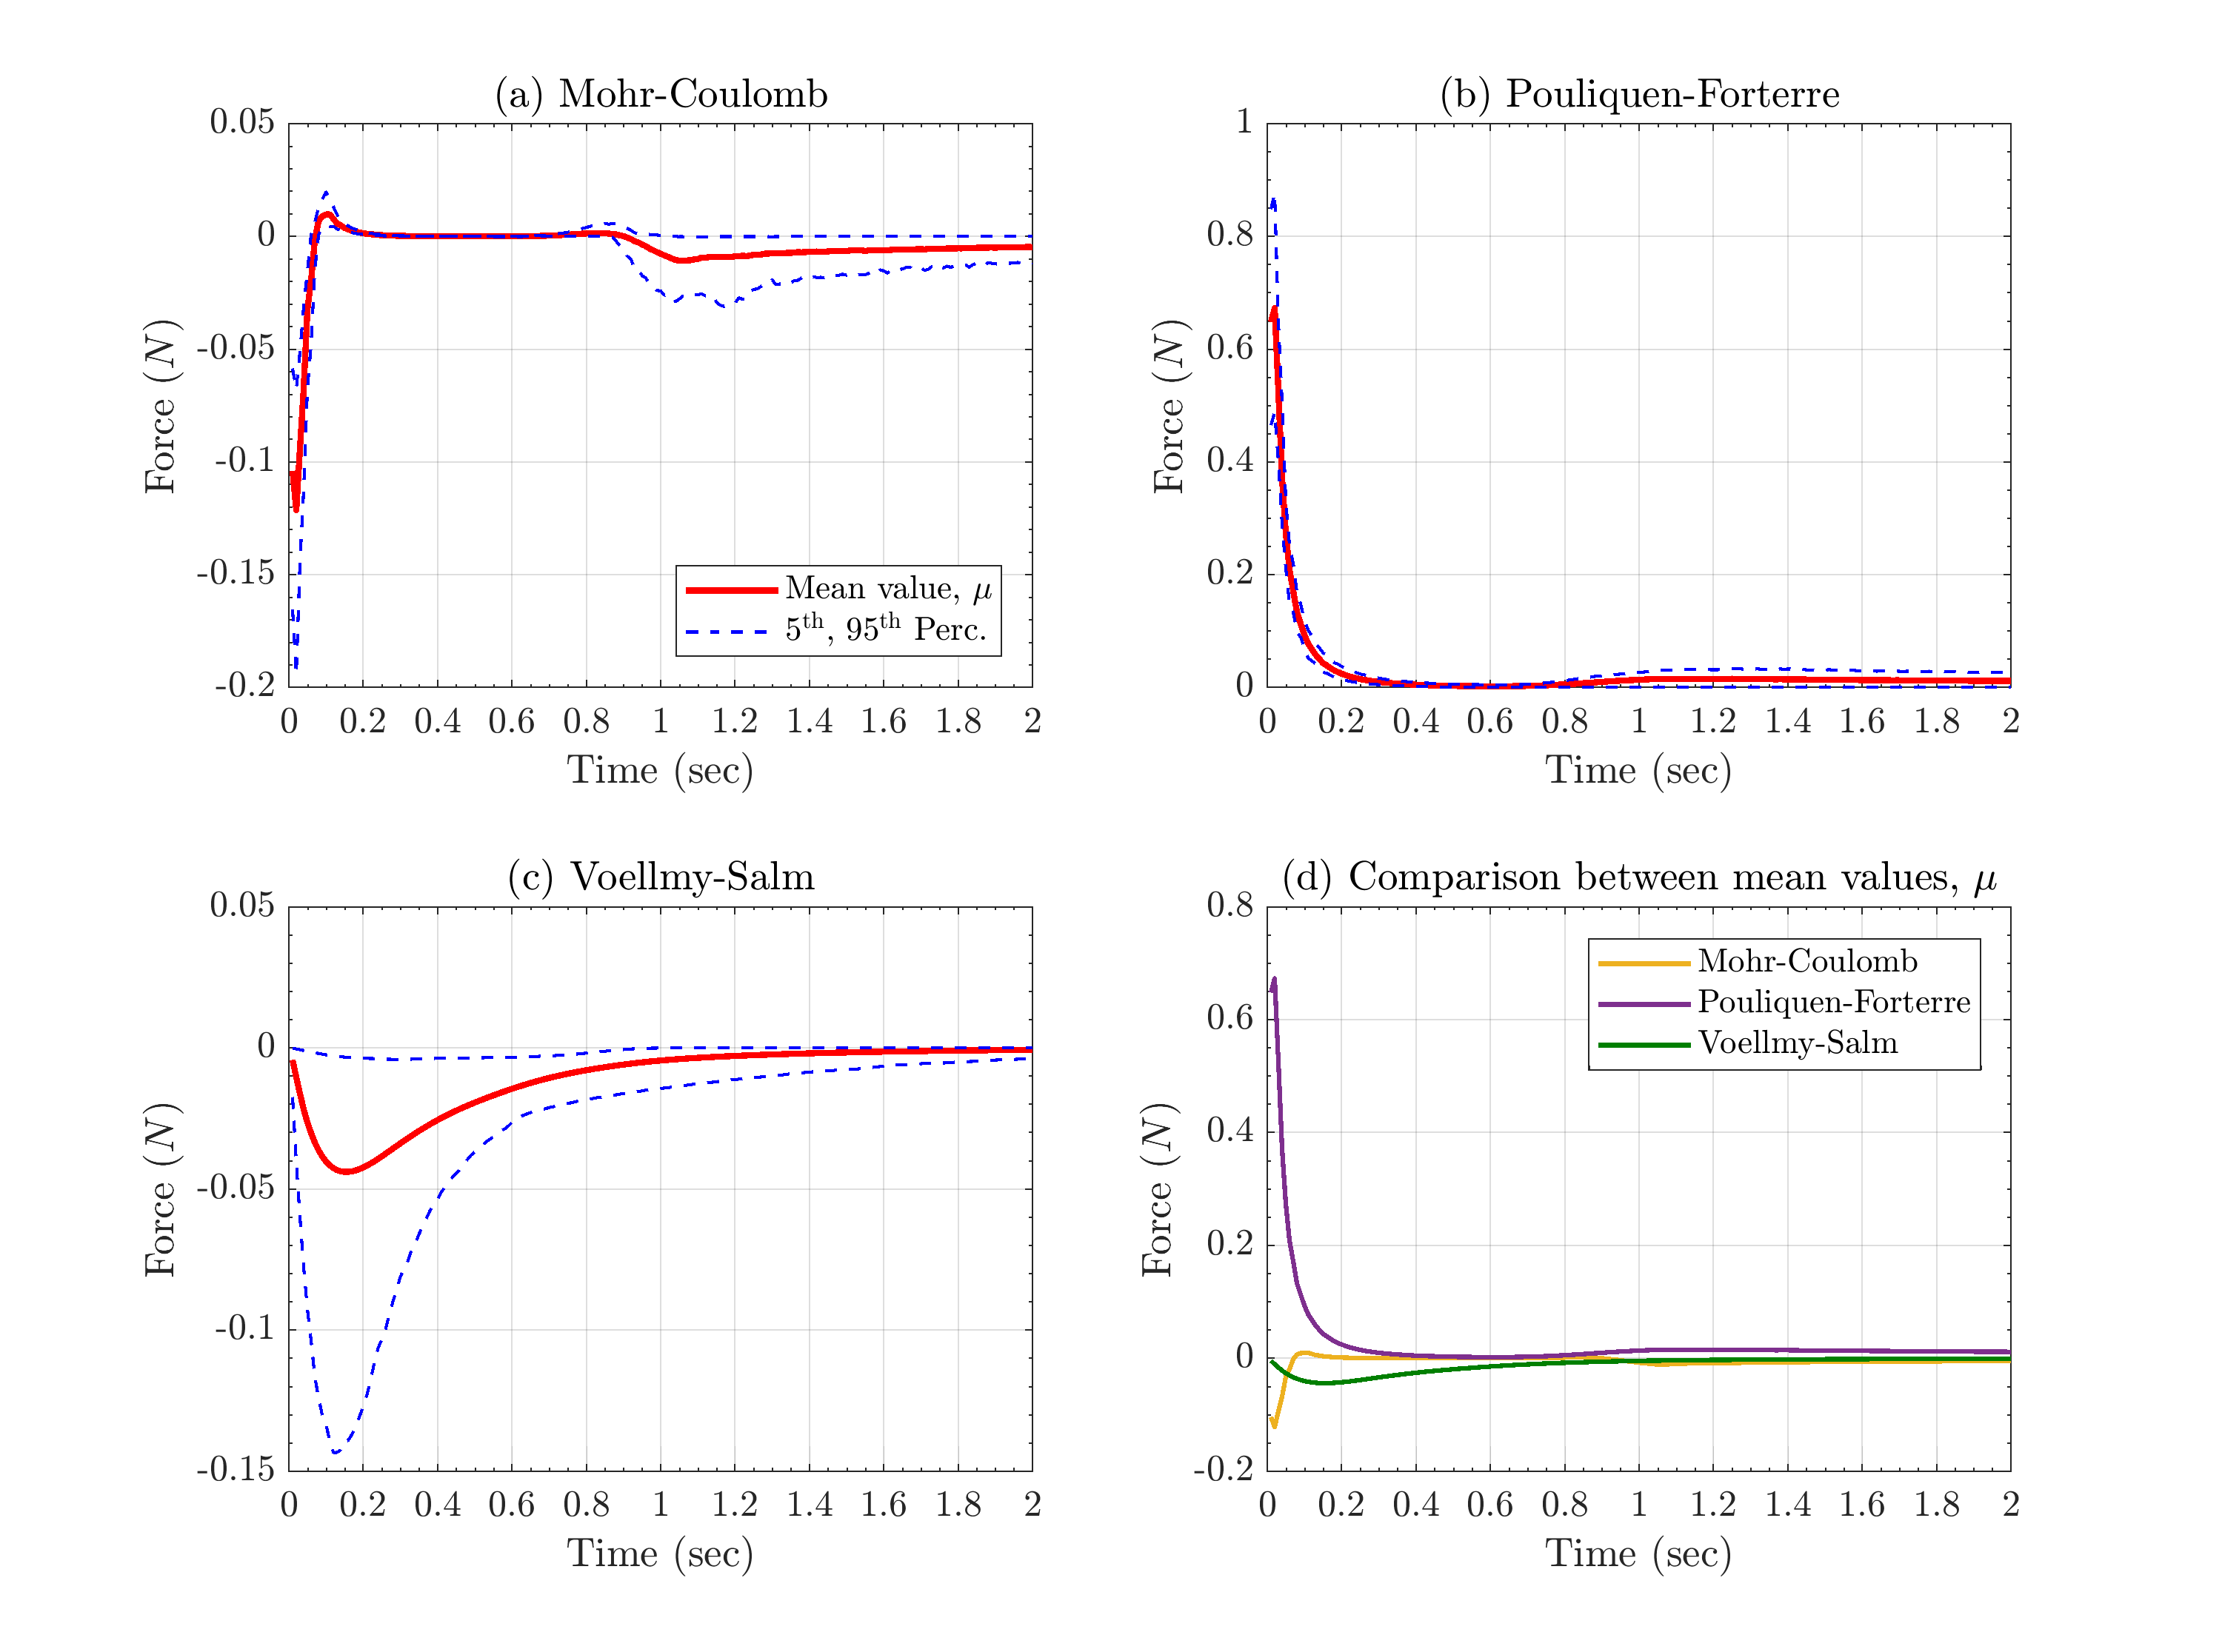
\includegraphics[width=1\textwidth]{InclinedPlane/Forces_Powers/RHS4/FRHS4y.png}
        \caption{Comparison between mean values of flow acceleration (computed from LHS), $\Vert \underline{a} \Vert(L,t)$, recorded at locations of interest, $L_i, \ _{i=1,...,4}$.}
        \label{fig:Ramp-RHS4-Fy-spatial}
\end{figure}

\begin{figure}[H]
        \centering
        \includegraphics[width=1\textwidth]{InclinedPlane/Forces_Powers/RHS4/PRHS4.png}
        \caption{Comparison between mean values of flow acceleration (computed from LHS), $\Vert \underline{a} \Vert(L,t)$, recorded at locations of interest, $L_i, \ _{i=1,...,4}$.}
        \label{fig:Ramp-RHS4-Power-spatial}
\end{figure}

\end{itemize}


\subsection{Statistical analysis of force contributions}
A statistical analysis capable of measuring the contributions of different force components in the rheology models is a fundamental task. This is also necessary to explore and compare the effects of the assumptions behind some modeling choices, onto the time evolution of the flowing material. Let $(F_i(x,t))_{i=1,\dots, n}$ be the array of force components, where $x\in\mathbb R^2$ is a spatial location, and $t\in T$ is a time instant. In our case study, $F_1$ is the gravitational force, $F_2$ is the basal friction, $F_3$ is the curvature correction, $F_4$ is a resistive force (or the hydrostatic pressure term, in the case of Pouliquen-Forterre rheology). However, this type of procedure can be applied to any additive decomposition of the physical forces. In addition, we can include in the analysis also the component of the inertial forces, i.e. $F_4$ the convective force and $F_5$ the transient force. The analysis of local effects can be compared to the contribution of global dynamics.

In this case we are projecting the forces on the directions X and Y, i.e. respectively in the slope direction, and orthogonal to the slope direction on an horizontal plane. Hence in the following the forces are scalar and not vectorial terms. It is important to remark that all the forces are depending on the sample $\eta$ on the parameter domains, and hence are considered as random variables.

The degree of contribution of those force terms is significantly variable in space and time. For this reason, the following analysis is performed on locally sampled measurements, and not in a spatial averaging framework. In particular, four locations are selected among the center line of the flow. These are: the initial pile location $x_1=-0.7$ m, the middle of the inclined plane $x_2=-0.35$ m, the change in slope $x_3=0$ m, the middle of the flat plane $x_4=0.15$ m. Next notation will assume to be in a selected location $x=x_k$, where $k\in\{1,\dots, 4\}$. The definitions are not depending on the location, but all the results will significantly depend of that choice.

\begin{definition}[Contribution coefficients]
Let $(F_i)_{i=1,\dots, n}$ be random variables on $(\Omega, \mathcal F, P)$, representing the considered force components in location $x$ at time $t$. Then, for each component $i$, the contribution coefficient is defined as:
$$C_i:=\mathbb E\left[\frac{F_i}{\Phi}\right],$$
where $\Phi$ is a dominating function, i.e. $\Phi\ge |F_i|$, $\forall i$.
\end{definition}
The \emph{total force}, i.e $\sum_i F_i$ excluding the inertial terms, is not a good candidate for a dominating function. Indeed, the terms often have opposite signs, and their sum can be really small. Another issue is given by the existence of a subset of times $\Theta$ characterized by the absence of flow in the selected location $x$. In $\Theta$ the dominant force is null, and cannot be the denominator of a fraction.

We explore two alternative $\Phi$ choices: $\Phi_1$ is based on the $l^1$ norm, and defined as:
$$\Phi_1:=\left\{
    \begin{array}{ll}
      \sum_i \frac{|F_i|}{2}, & \hbox{if not null;} \\
      1, & \hbox{otherwise.}
    \end{array}
  \right.$$
In case we exclude the inertial forces from the analysis, we must take $\hat{\Phi_1}=2\Phi_1$. In contrast $\Phi_2$ is the dominant force, based on the $l^\infty$ norm:
$$\Phi_2:=\left\{
    \begin{array}{ll}
      \max_i |F_i|, & \hbox{if not null;} \\
      1, & \hbox{otherwise.}
    \end{array}
  \right.$$
In particular, for a particular location $x$, time $t$, and parameter sample $\eta$, we have $C_i=0$ if there is no flow or all the forces are null. The expectation of $C_i$ is reduced by the chance of $F_i$ being small compared to the other terms, or by the chance of having no flow in $(x,t)$. Moreover, $\mathbb E[C_i]\in[-1,1]$, $\forall i$.
\begin{proposition}
Let $\Phi_k$, $k=1,2$ be the functions described above. Then they are well defined dominating function, i.e. $\Phi_k\ge |F_j|$, $\forall j,k$.
\end{proposition}
\begin{proof}
If $k=1$, the Newton equation states $\sum_{j\in J} F_j =\sum_{i\in I} F_i,$ where $(F_j)_{j\in J}$ are inertial forces, and $(F_i)_{i\in I}$ the local forces. Then, $\forall h\in I$
$$F_h=\sum_{i\neq h,\ i\in I} F_i - \sum_{j\in J} F_j.$$
And hence
$$|F_h|\le |F_h|+\sum_{i\neq k,\ i\in I} |F_i| - \sum_{j\in J} |F_j|=2\Phi_1.$$
A similar equation is valid $\forall k\in J$. If $k=2$, or if the inertial forces are not included, the proof is trivial.
\end{proof}

Furthermore, assuming $\Phi=\Phi_2$, there is a useful result explaining the meaning of those coefficients through the conditional expectation.
\begin{proposition}
Let $(F_i)_{i=1,\dots, n}$ be random variables on $(\Omega, \mathcal F, P)$, representing the considered force components in location $x$ at time $t$. For each $i$, let $C_i$ be the contribution coefficient of force $F_i$, assuming $\Phi=\Phi_2$. Then we have the following expression:
$$C_i=\sum_j p_j \mathbb E\left[\frac{F_i}{|F_j|}\ \Big{|}\ \Phi=|F_j|\right],$$
where $p_j:=P\left\{\Phi=|F_j|\right\}$.
\end{proposition}

\begin{proof}
Let $Z$ be a discrete random variable such that, for each $j\in\mathbb N$, $(Z=j) \Longleftrightarrow (\Phi=|F_j|)$. Then, by the rule of chain expectation:
$$C_i=\mathbb E\left[\frac{F_i}{\Phi}\right]=\mathbb E\left[\mathbb E\left[\frac{F_i}{\Phi}\ \Big{|}\ Z=j\right]\right]=$$
$$=\mathbb E\left[\mathbb E\left[\frac{F_i}{|F_j|}\ \Big{|}\ Z=j\right]\right]=\sum_j P\left\{Z=j\right\} \mathbb E\left[\frac{F_i}{|F_j|}\ \Big{|}\ Z=j\right].$$
Moreover, by definition, $p_j=P\left\{Z=j\right\}$. This completes the proof.
\end{proof}

The last proposition brings to the definition of the dominance factors $(p_j)_{j=1,\dots, k}$, i.e. the probability of each $F_j$ to be the dominant force in $(x,t)$.

\begin{definition}[Dominance factors and conditional contributions]
Let $(F_i)_{i=1,\dots, k}$ be random variables on $(\Omega, \mathcal F, P)$, representing arbitrary force components in location $x$ at time $t$. Then, for each pair of components $(i,j)$, the conditional contribution $C_{i,j}$ is defined as:
$$C_{i,j}:=\mathbb E\left[\frac{F_i}{|F_j|}\ \Big{|}\ \Phi=|F_j|\right],$$
where $\Phi=\Phi_2$ is the dominant force. In particular, for each component $i$, the dominance factor is defined as:
$$p_j:=P\left\{\Phi=|F_j|\right\}.$$
\end{definition}

In the following we display the contribution coefficients barplots as a function of time, for the locations $x_1,\dots,x_4$ defined above. Moreover, we report the dominance factors plots, a very useful tool to read the dynamical significance of the forces as a function of time and location.


\begin{figure}[H]
        \centering
        \includegraphics[width=1\textwidth]{InclinedPlane/LocalRecords/DominancePrX_L1.png}
        \caption{Probability of events $(C_i)_{i=1,...,6}:=\left\{\Phi_2=|F_i|\right\}$ for the \emph{Mohr-Coulomb} model, $(P_i)_{i=1,...,6}:=\left\{\Phi_2=|F_i|\right\}$ for the \emph{Pouliquen-Forterre} model, $(V_i)_{i=1,...,6}:=\left\{\Phi_2=|F_i|\right\}$ for \emph{Voellmy-Salm} model, where $F_1$ is the \emph{transient force}, $F_2$ the \emph{convective force}, $F_3$ the \emph{gravitational force}, $F_4$ the \emph{basal friction force}, $F_5$ the \emph{curvature based basal friction force}, and $F_6$ the \emph{resisting force} (or the hydrostatic pressure term, in the case of Pouliquen-Forterre rheology). Moreover, $C_7,\ P_7,\ V_7$ correspond to the event of \emph{no flow}. All the measurements were recorded at $L_1=(-0.7,0)$ and along the runout direction.}
        \label{fig:Ramp-FXDominance-L1}
\end{figure}

\begin{figure}[H]
        \centering
        \includegraphics[width=1\textwidth]{InclinedPlane/LocalRecords/DominancePrY_L1.png}
        \caption{Probability of events $(C_i)_{i=1,...,6}:=\left\{\Phi_2=|F_i|\right\}$ for the \emph{Mohr-Coulomb} model, $(P_i)_{i=1,...,6}:=\left\{\Phi_2=|F_i|\right\}$ for the \emph{Pouliquen-Forterre} model, $(V_i)_{i=1,...,6}:=\left\{\Phi_2=|F_i|\right\}$ for \emph{Voellmy-Salm} model, where $F_1$ is the \emph{transient force}, $F_2$ the \emph{convective force}, $F_3$ the \emph{gravitational force}, $F_4$ the \emph{basal friction force}, $F_5$ the \emph{curvature based basal friction force}, and $F_6$ the \emph{resisting force} (or the hydrostatic pressure term, in the case of Pouliquen-Forterre rheology). Moreover, $C_7,\ P_7,\ V_7$ correspond to the event of \emph{no flow}. All the measurements were recorded at $L_1=(-0.7,0)$ and along the lateral direction.}
        \label{fig:Ramp-FYDominance-L1}
\end{figure}

\begin{figure}[H]
        \centering
        \includegraphics[width=1\textwidth]{InclinedPlane/LocalRecords/DominancePrX_L2.png}
        \caption{Probability of events $(C_i)_{i=1,...,6}:=\left\{\Phi_2=|F_i|\right\}$ for the \emph{Mohr-Coulomb} model, $(P_i)_{i=1,...,6}:=\left\{\Phi_2=|F_i|\right\}$ for the \emph{Pouliquen-Forterre} model, $(V_i)_{i=1,...,6}:=\left\{\Phi_2=|F_i|\right\}$ for \emph{Voellmy-Salm} model, where $F_1$ is the \emph{transient force}, $F_2$ the \emph{convective force}, $F_3$ the \emph{gravitational force}, $F_4$ the \emph{basal friction force}, $F_5$ the \emph{curvature based basal friction force}, and $F_6$ the \emph{resisting force} (or the hydrostatic pressure term, in the case of Pouliquen-Forterre rheology). Moreover, $C_7,\ P_7,\ V_7$ correspond to the event of \emph{no flow}. All the measurements were recorded at $L_2=(-0.35,0)$ and along the runout direction.}
        \label{fig:Ramp-FXDominance-L2}
\end{figure}

\begin{figure}[H]
        \centering
        \includegraphics[width=1\textwidth]{InclinedPlane/LocalRecords/DominancePrY_L2.png}
        \caption{Probability of events $(C_i)_{i=1,...,6}:=\left\{\Phi_2=|F_i|\right\}$ for the \emph{Mohr-Coulomb} model, $(P_i)_{i=1,...,6}:=\left\{\Phi_2=|F_i|\right\}$ for the \emph{Pouliquen-Forterre} model, $(V_i)_{i=1,...,6}:=\left\{\Phi_2=|F_i|\right\}$ for \emph{Voellmy-Salm} model, where $F_1$ is the \emph{transient force}, $F_2$ the \emph{convective force}, $F_3$ the \emph{gravitational force}, $F_4$ the \emph{basal friction force}, $F_5$ the \emph{curvature based basal friction force}, and $F_6$ the \emph{resisting force} (or the hydrostatic pressure term, in the case of Pouliquen-Forterre rheology). Moreover, $C_7,\ P_7,\ V_7$ correspond to the event of \emph{no flow}. All the measurements were recorded at $L_2=(-0.35,0)$ and along the lateral direction.}
        \label{fig:Ramp-FYDominance-L2}
\end{figure}

\begin{figure}[H]
        \centering
        \includegraphics[width=1\textwidth]{InclinedPlane/LocalRecords/DominancePrX_L3.png}
        \caption{Probability of events $(C_i)_{i=1,...,6}:=\left\{\Phi_2=|F_i|\right\}$ for the \emph{Mohr-Coulomb} model, $(P_i)_{i=1,...,6}:=\left\{\Phi_2=|F_i|\right\}$ for the \emph{Pouliquen-Forterre} model, $(V_i)_{i=1,...,6}:=\left\{\Phi_2=|F_i|\right\}$ for \emph{Voellmy-Salm} model, where $F_1$ is the \emph{transient force}, $F_2$ the \emph{convective force}, $F_3$ the \emph{gravitational force}, $F_4$ the \emph{basal friction force}, $F_5$ the \emph{curvature based basal friction force}, and $F_6$ the \emph{resisting force} (or the hydrostatic pressure term, in the case of Pouliquen-Forterre rheology). Moreover, $C_7,\ P_7,\ V_7$ correspond to the event of \emph{no flow}. All the measurements were recorded at $L_3=(0,0)$ and along the runout direction.}
        \label{fig:Ramp-FXDominance-L3}
\end{figure}

\begin{figure}[H]
        \centering
        \includegraphics[width=1\textwidth]{InclinedPlane/LocalRecords/DominancePrY_L3.png}
        \caption{Probability of events $(C_i)_{i=1,...,6}:=\left\{\Phi_2=|F_i|\right\}$ for the \emph{Mohr-Coulomb} model, $(P_i)_{i=1,...,6}:=\left\{\Phi_2=|F_i|\right\}$ for the \emph{Pouliquen-Forterre} model, $(V_i)_{i=1,...,6}:=\left\{\Phi_2=|F_i|\right\}$ for \emph{Voellmy-Salm} model, where $F_1$ is the \emph{transient force}, $F_2$ the \emph{convective force}, $F_3$ the \emph{gravitational force}, $F_4$ the \emph{basal friction force}, $F_5$ the \emph{curvature based basal friction force}, and $F_6$ the \emph{resisting force} (or the hydrostatic pressure term, in the case of Pouliquen-Forterre rheology). Moreover, $C_7,\ P_7,\ V_7$ correspond to the event of \emph{no flow}. All the measurements were recorded at $L_3=(0,0)$ and along the lateral direction.}
        \label{fig:Ramp-FYDominance-L3}
\end{figure}

\begin{figure}[H]
        \centering
        \includegraphics[width=1\textwidth]{InclinedPlane/LocalRecords/DominancePrX_L4.png}
        \caption{Probability of events $(C_i)_{i=1,...,6}:=\left\{\Phi_2=|F_i|\right\}$ for the \emph{Mohr-Coulomb} model, $(P_i)_{i=1,...,6}:=\left\{\Phi_2=|F_i|\right\}$ for the \emph{Pouliquen-Forterre} model, $(V_i)_{i=1,...,6}:=\left\{\Phi_2=|F_i|\right\}$ for \emph{Voellmy-Salm} model, where $F_1$ is the \emph{transient force}, $F_2$ the \emph{convective force}, $F_3$ the \emph{gravitational force}, $F_4$ the \emph{basal friction force}, $F_5$ the \emph{curvature based basal friction force}, and $F_6$ the \emph{resisting force} (or the hydrostatic pressure term, in the case of Pouliquen-Forterre rheology). Moreover, $C_7,\ P_7,\ V_7$ correspond to the event of \emph{no flow}. All the measurements were recorded at $L_4=(0.15,0)$ and along the runout direction.}
        \label{fig:Ramp-FXDominance-L4}
\end{figure}

\begin{figure}[H]
        \centering
        \includegraphics[width=1\textwidth]{InclinedPlane/LocalRecords/DominancePrY_L4.png}
        \caption{Probability of events $(C_i)_{i=1,...,6}:=\left\{\Phi_2=|F_i|\right\}$ for the \emph{Mohr-Coulomb} model, $(P_i)_{i=1,...,6}:=\left\{\Phi_2=|F_i|\right\}$ for the \emph{Pouliquen-Forterre} model, $(V_i)_{i=1,...,6}:=\left\{\Phi_2=|F_i|\right\}$ for \emph{Voellmy-Salm} model, where $F_1$ is the \emph{transient force}, $F_2$ the \emph{convective force}, $F_3$ the \emph{gravitational force}, $F_4$ the \emph{basal friction force}, $F_5$ the \emph{curvature based basal friction force}, and $F_6$ the \emph{resisting force} (or the hydrostatic pressure term, in the case of Pouliquen-Forterre rheology). Moreover, $C_7,\ P_7,\ V_7$ correspond to the event of \emph{no flow}. All the measurements were recorded at $L_4=(0.15,0)$ and along the lateral direction.}
        \label{fig:Ramp-FYDominance-L4}
\end{figure}


\section{Volc{\'a}n de Colima block and ash flow.}
The parameter ranges adopted in this case study are:

\vskip.3cm\noindent \textbf{MC} - $\phi_{bed} \in [10^{\mathrm{\circ}}, 25^{\mathrm{\circ}}]$ \citep{Dalbey2008, Spiller2014}, $\quad \Delta\phi \in [2^{\mathrm{\circ}}, 10^{\mathrm{\circ}}]$.

\vskip.3cm\noindent \textbf{PF} - $\phi_2 \in [10^{\mathrm{\circ}}, 30^{\mathrm{\circ}}]$, $\quad\Delta\phi_{12} \in [5^{\mathrm{\circ}}, 15^{\mathrm{\circ}}]$, $\quad\beta \in [0.1, 0.85]$, $\quad L=10^{-1} \ (m)$, $\quad \phi_3=\phi_1 + 1^{\mathrm{\circ}}$.

\vskip.3cm\noindent \textbf{VS} - $\mu \in [0.15, 0.55]$, $\quad \log(\xi) \in [1.7, 4]$.


\section{Results and Discussion}

\section*{Appendix A: Latin Hypercubes and orthogonal arrays}
The Latin Hypercube Sampling (LHS) is a well established procedure for defining pseudo-random designs of samples in $\mathbb R^d$, with good properties with respect to the uniform probability distribution on an hypercube $[0,1]^d$ \citep{McKay1979,Owen1992b,Stein1987,Ranjan2014,Mingyao2016}. In particular, compared to a random sampling, a LHS: (i) enhances the capability to fill the d-dimensional space with a finite number of points, (ii) in case $d>1$, avoids the overlapping of point locations in the one dimensional projections, (iii) reduces the dependence of the number of points necessary on the dimensionality $d$.

\begin{definition}[Latin hypercube sampling]
Let $\Xi=\{\xi_i\ :\ i=1,\dots,N\}$ be a set of points inside the d-dimensional hypercube $C=[0,1]^d$. Let $[0,1]=\bigcup_{j=1}^{N} I_j$, where $I_j=[\frac{(j-1)}{N},\frac{j}{N}]$. Let $\xi_i=\left(\xi_i^1,\dots,\xi_i^d\right)$, and for each $k\in\{1,\dots,d\}$, let $\Xi^k=\{\xi^k_i\ :\ i=1,\dots,N\}$. Let $\lambda^d$ be the uniform probability measure supported inside $C$, called Lebesgue measure. Then $\Xi$ is a latin hypercube w.r.t. $\lambda^d$ $\Longleftrightarrow$ $\forall j\in \{1,\dots,N\}$, $\forall k\in\{1,\dots,d\}$, $\left|I_j\cap\Xi^k\right|=1$.
\end{definition}

The procedure is simple: once the desired number of samples $N\in\mathbb N$ is selected, and $[0,1]$ is divided in $N$ equal bins, then each bin will contain one and only one projection of the samples over every coordinate. The LHS definition is trivially generalized over $C=\prod^d_i [a_i, b_i]$, i.e. the cartesian product of $d$ arbitrary intervals. That will be applied in this study, defining LHS over the parameter domain of the flow models.

There are a large number of possible designs, corresponding the number of permutations of the bins in the d-projections, i.e. $d\cdot N!$. If the permutations are randomly sampled there is a high possibility that the design will have good properties. However, this is not assured, and clusters o points or regions of void space may be observed in $C$. For this reason, we base our design on the orthogonal arrays (OA) \citep{Owen1992a,Tang1993}.

\begin{definition}[Orthogonal arrays]
Let $S=\{1,\dots,s\}$, where $s\ge 2$. Let $Q\in S^{n\times m}$ be a matrix of such integer values. Then $Q$ is called an $OA(n,m,s,r)$ $\Longleftrightarrow$ each $n\times r$ submatrix of $Q$ contains all possible $1\times r$ row vectors with the same frequency $\lambda=n/s^r$, which is called the index of the array. In particular, $r$ is called the strength, $n$ the size, $(m\ge r)$ the constrains, and $s$ the levels of the array.
\end{definition}

Orthogonal arrays are very useful for defining latin hypercubes which are also forced to fill the space (or its r-dimensional subspaces) in a more robust way, at the cost of potentially requiring a larger number of points than a traditional LHS.

\begin{proposition}
Let $Q$ be an $OA(n,m,s,r)$. Then let $U\in\mathbb R^{n\times m}$ be defined as follows:
$$\forall k\in \{1,\dots,s\},\ \forall j\in \{1,\dots,m\},\ \left\{Q[\cdot,j]\ :\ Q[i,j]=k\right\} = \Pi\left(\{(k-1)\lambda s^{r-1},\dots, k\lambda s^{r-1}\}\right),$$
where $\Pi$ is a random permutation of $\lambda s^{r-1}$ elements. Then $\Xi=\{\xi_i=U[i,\cdot]\ :\ i=1,\dots,n\}$ is a LHS w.r.t to $\lambda^m$ over $C=[0,1]^m$. Moreover, let $[0,1]^r=\bigcup_{(h_1,\dots,h_r)=1}^{s} I_{(h_i)}$, where $I_{(h_i)}=\prod^r_i[\frac{(h_i-1)}{s},\frac{h_i}{s}]$. Then $\forall D=(d_1,\dots,d_r)\subseteq \{1,\dots,m\}$, let $\Xi^D=\{(\xi^{d_1},\dots,\xi^{d_r})\ :\ i=1,\dots,n\}$. We have that
$$\forall k\in \{1,\dots,s\},\ \forall (h_i\ : i=1,\dots,r)\in\{1,\dots,d\}^r,\ \left|I_{(k_i)}\cap\Xi^D\right|=\lambda.$$
\end{proposition}

For each column of $Q$ we are replacing the $\lambda s^{r-1}$ elements with entry $k$ by a random permutation of $\left((k-1)\lambda s^{r-1} + h\right)_{h\in 1,\dots, \lambda s^{r-1}}$. After the replacement procedure is done, the newly obtained matrix $U$ is equivalent to a LHS which inherits from $Q$ the property of fully covering $s^r$ equal r-dimensional hypercubes in every r-dimensional projection. Each hypercube contains $\lambda$ points. In other words, inside each r-dimensional projection, the design associated to $U$ fills the space like a regular grid at the scale of those $s^r$ hypercubes, but it is still an LHS at a finer scale, i.e. the $\lambda s^{r-1}$ one dimensional bins. A complete proof can be found in \cite{Tang1993} and it is a straightforward verification of the required properties.

However, even in an LHS based on an $OA(n,m,s,r)$, if $r<m$ what happens in the projections with dimension $r'>r$ is not controlled, and randomizing procedures are made more difficult by the additional structure imposed by the $OA$. Moreover, the total number of points necessary to achieve a full design increases with $r$, and hence is affected by dimensionality issues.

Dealing with relatively small $d$, i.e. $d\in\{3,4\}$, we adopt a LHS $U$ created by a $OA(s^d,d,s,d)$. The strength is equal to the dimension $d$, hence the design fills the entire space like a $d$ dimensional grid, but it is a LHS as well. In this case there is one point in each hypercube, and $\lambda=1$. We take $s=8$ for the 3-dimensional designs over the parameter space of Mohr-Coulomb and Voellmy-Salm models, i.e. $512$ points; we took $s=6$ for the 4-dimensional designs over the more complex parameter space of the Pouliquen-Forterre model, i.e. 1296 points.

\newpage
\bibliographystyle{apa}
\bibliography{mybibfile}

\end{document}
